\documentclass[11pt,oneside]{book}
\usepackage{fontspec}
\setmainfont{Noto Serif}
\setsansfont{Noto Sans}
\setmonofont{Noto Sans Mono}
\newfontfamily\proseunicodefont{DejaVu Serif}
\usepackage[margin=1in]{geometry}
\usepackage{microtype}
\usepackage{amsmath,amssymb,amsthm,mathtools,bm}
\usepackage{graphicx}
\usepackage{xcolor}
\usepackage{booktabs}
\usepackage{array}
\usepackage{longtable}
\usepackage{enumitem}
\usepackage{float}
\usepackage{caption}
\usepackage{hyperref}
\usepackage{fancyhdr}
\usepackage{tikz}
\usetikzlibrary{arrows.meta,positioning,calc,decorations.pathmorphing}

\hypersetup{
  colorlinks=true,
  linkcolor=blue!50!black,
  urlcolor=blue!50!black,
  citecolor=blue!50!black
}

\setlength{\parskip}{0.5em}
\setlength{\parindent}{0pt}
\setlist[itemize]{topsep=0.25em,itemsep=0.2em}
\setlist[enumerate]{topsep=0.25em,itemsep=0.2em}
\setlength{\headheight}{40pt}
\numberwithin{equation}{chapter}

\newtheorem{theorem}{Satz}[chapter]
\newtheorem{proposition}[theorem]{Proposition}
\newtheorem{lemma}[theorem]{Lemma}
\newtheorem{corollary}[theorem]{Korollar}
\theoremstyle{definition}
\newtheorem{definition}[theorem]{Definition}
\newtheorem{example}[theorem]{Beispiel}
\theoremstyle{remark}
\newtheorem{remark}[theorem]{Bemerkung}

\providecommand{\ket}[1]{\left\lvert#1\right\rangle}
\providecommand{\bra}[1]{\left\langle#1\right\rvert}
\providecommand{\braket}[2]{\left\langle#1\,\middle|\,#2\right\rangle}
\providecommand{\expect}[1]{\left\langle#1\right\rangle}
\newcommand{\lectureoverview}[1]{\paragraph{Überblick.} #1}
\newenvironment{classroomqa}{%
  \par\medskip
  \begin{quote}\small
}{%
  \end{quote}
  \medskip
}
\newcommand{\audiencequestion}[1]{\noindent\textbf{Frage aus dem Publikum.} #1\par\smallskip}
\newcommand{\classquestion}[1]{\noindent\textbf{Frage an den Kurs.} #1\par\smallskip}
\newcommand{\lecturerresponse}[1]{\noindent\textbf{Antwort.} #1\par}
\newcommand{\lecturetimestamp}[1]{\footnote{Vorlesungszeit: #1.}}
\newcommand{\lectureframe}[1]{\par\smallskip{\centering\footnotesize\itshape Vorlesungsbild: #1.\par}}

\makeatletter
\newcommand{\course@headerfont}{\normalfont\small\itshape}
\newcommand{\course@pagefont}{\normalfont\small}
\newcommand{\course@headerraise}{14pt}
\newlength{\course@headerboxheight}
\setlength{\course@headerboxheight}{\dimexpr\headheight-\course@headerraise-9pt\relax}
\newcommand{\course@leftheadbox}[1]{%
  \raisebox{\course@headerraise}{%
    \parbox[t][\course@headerboxheight][t]{0.82\textwidth}{%
      \raggedright\course@headerfont\strut\MakeUppercase{#1}\strut%
    }%
  }%
}
\newcommand{\course@rightheadbox}[1]{%
  \raisebox{\course@headerraise}{%
    \parbox[t][\course@headerboxheight][t]{0.82\textwidth}{%
      \raggedleft\course@headerfont\strut\MakeUppercase{#1}\strut%
    }%
  }%
}
\renewcommand{\chaptermark}[1]{\markboth{\MakeUppercase{\chaptername\ \thechapter.\ #1}}{}}
\renewcommand{\sectionmark}[1]{\markright{\MakeUppercase{\thesection\hspace{0.4em}#1}}}
\fancyhf{}
\fancyhead[L]{\course@leftheadbox{\leftmark}}
\fancyhead[R]{\course@pagefont\thepage}
\renewcommand{\headrulewidth}{0.5pt}
\pagestyle{fancy}
\fancypagestyle{plain}{%
  \fancyhf{}
  \fancyhead[L]{\course@leftheadbox{\leftmark}}
  \fancyhead[R]{\course@pagefont\thepage}
  \renewcommand{\headrulewidth}{0.5pt}
}
\makeatother

\usepackage{polyglossia}
\setdefaultlanguage{german}
\usepackage{sectsty}
\renewcommand{\contentsname}{Inhaltsverzeichnis}
\renewcommand{\chaptername}{Kapitel}
\renewcommand{\figurename}{Abbildung}
\renewcommand{\tablename}{Tabelle}
\renewcommand{\proofname}{Beweis}
\renewcommand{\bibname}{Literatur}
\sectionfont{\raggedright}
\subsectionfont{\raggedright}
\makeatletter
\renewcommand{\@pnumwidth}{2.2em}
\renewcommand{\@tocrmarg}{3.2em}
\makeatother
\usepackage{tocloft}
\renewcommand{\cftchapfont}{\small\bfseries}
\renewcommand{\cftchappagefont}{\small\bfseries}
\renewcommand{\cftsecfont}{\small}
\renewcommand{\cftsecpagefont}{\small}
\setlength{\cftsecnumwidth}{3em}
\renewcommand{\cftsubsecfont}{\small}
\renewcommand{\cftsubsecpagefont}{\small}
\setlength{\cftsubsecindent}{4.5em}
\setlength{\cftsubsecnumwidth}{4em}
\emergencystretch=6em
\pdfstringdefDisableCommands{\def\proseunicodefont{}}

\geometry{paperwidth=177.6mm,paperheight=252mm,left=16mm,right=16mm,
 top=18mm,bottom=18mm,includeheadfoot,headheight=28pt,headsep=7mm,footskip=9mm}
\usepackage{scrextend}
\changefontsizes[17pt]{12pt}
\raggedbottom
\renewenvironment{classroomqa}{\par\medskip\begingroup}{\par\endgroup\medskip}
\fancyhf{}
\setlength{\headwidth}{\textwidth}
\fancyhead[L]{\parbox{\textwidth}{\raggedright\fontsize{9}{11}\selectfont\nouppercase{\leftmark}}}
\fancyfoot[C]{\small\thepage}
\renewcommand{\headrulewidth}{0.3pt}
\fancypagestyle{plain}{\fancyhf{}\fancyfoot[C]{\small\thepage}\renewcommand{\headrulewidth}{0pt}}

\graphicspath{{../../../generated_course_notes/core/statistical_mechanics/2013_spring_theoretical_minimum/figures/}{../../../generated_course_notes/core/statistical_mechanics/2013_spring_theoretical_minimum/assets/}}
\hypersetup{
  pdftitle={Statistical Mechanics: The Theoretical Minimum},
  pdfauthor={Leonard Susskind; companion notes edited by LazyingArt LLC with Video2Book},
  pdfsubject={Core track, 2013 Spring},
  pdfkeywords={Leonard Susskind, statistical mechanics, thermodynamics, Ising model, critical phenomena}
}
\begin{document}
\frontmatter
\hypersetup{pageanchor=false}
\begin{titlepage}
\hyphenpenalty=10000\exhyphenpenalty=10000
\thispagestyle{empty}
\begin{tikzpicture}[remember picture,overlay]
  \node[anchor=south west,inner sep=0] at (current page.south west) {%
    \includegraphics[width=\paperwidth,height=\paperheight,keepaspectratio=false]{../../../generated_course_notes/core/statistical_mechanics/2013_spring_theoretical_minimum/assets/cover-art.png}%
  };
  \node[
    anchor=north west,
    align=left,
    text width=0.78\paperwidth,
    fill=white,
    fill opacity=0.9,
    rounded corners=8pt,
    inner xsep=10pt,
    inner ysep=8pt
  ] at ([xshift=0.08\paperwidth,yshift=-0.06\paperheight]current page.north west) {%
    {\fontsize{30}{33}\selectfont\bfseries\color{black!88} Statistische Mechanik\\[0.85em]}
    {\large\color{black!72} Deutsche Ausgabe / Frühjahr 2013, Theoretisches Minimum}
  };
  \node[
    anchor=south west,
    align=left,
    text width=0.68\paperwidth,
    fill=white,
    fill opacity=0.82,
    text opacity=1,
    rounded corners=6pt,
    inner sep=12pt
  ] at ([xshift=0.08\paperwidth,yshift=0.08\paperheight]current page.south west) {%
    {\normalsize\color{black!78} Originalvorlesungen: Leonard Susskind\\[0.35em]}
    {\small\color{black!72} Begleitausgabe: \href{https://lazying.art}{LazyingArt LLC} / \href{https://github.com/lachlanchen/Video2Book}{Video2Book}.}
  };
\end{tikzpicture}
\mbox{}
\end{titlepage}
\hypersetup{pageanchor=true}

\chapter{Zu diesen Notizen}
Diese unabhängig bearbeiteten Begleitnotizen folgen den Vorlesungen 2013 zur Statistischen Mechanik von Leonard Susskind. Sie bewahren die erklärende Reihenfolge der Vorlesungen, wesentliche Gespräche im Hörsaal, mathematische Herleitungen und ausgewählte Tafelanschriebe. Sie sind kein Originalmanuskript von Professor Susskind und wurden von ihm weder geprüft noch gebilligt.

Die Ausgabe wurde von \href{https://lazying.art}{LazyingArt LLC} mit dem Open-Source-Workflow \href{https://github.com/lachlanchen/Video2Book}{Video2Book} erstellt. Vollständige maschinell erstellte Transkripte und Untertiteldateien stehen separat im Repository zur Verfügung und können Erkennungsfehler enthalten.
\clearpage
\tableofcontents
\mainmatter
\chapter{Wahrscheinlichkeit, Information und Entropie}

\lectureoverview{Die statistische Mechanik beginnt dort, wo mikroskopische Gesetze auf unvollständiges Wissen treffen. Zunächst präzisieren wir den Wahrscheinlichkeitsbegriff. Dann fragen wir, wie die deterministische Bewegung selbst Wahrscheinlichkeiten festlegt, wie Erhaltungssätze den Zustandsraum aufteilen und warum informationsbewahrende Dynamik ganz natürlich zur Entropie führt. Der erste und der nullte Hauptsatz kommen erst ins Spiel, wenn diese Struktur steht.}

\section{Warum statistische Mechanik?}

Die statistische Mechanik wird manchmal als alte Physik bezeichnet. Das verfehlt den entscheidenden Punkt. Sie ist vormodern, modern und wird wohl auch in jeder postmodernen Physik nützlich bleiben, die auf die uns bekannten Theorien folgt. Einzelne Modelle kommen und gehen; der zweite Hauptsatz der Thermodynamik hat sich wiederholt als verlässlicher Wegweiser erwiesen. Wann immer eine vorgeschlagene Beschreibung der Natur scheinbar kostenlos Ordnung erzeugt, Information grundlegend auslöscht oder ein abgeschlossenes System in einen unnatürlich einfachen Zustand überführt, warnt uns der zweite Hauptsatz, dass etwas fehlt.

Das Fach mag weniger glamourös erscheinen als ein neu entdecktes Teilchen, ist aber mindestens ebenso tiefgründig und wesentlich allgemeiner. Gase, Flüssigkeiten, Festkörper, Strahlung, Schwarze Löcher, Information und Quantenfelder erfordern statistisches Denken. Tatsächlich ließe sich die experimentelle Technik, mit der Teilchen entdeckt werden, ohne dieses Denken gar nicht verstehen. Deshalb haben Generationen herausragender Physikerinnen und Physiker die statistische Mechanik gemeistert, auch wenn ihr Hauptarbeitsgebiet anderswo lag: Das Fach ist nützlich, aber auch ungewöhnlich schön.

Um zu sehen, warum sie gebraucht wird, beginnen wir mit dem Ideal der Mechanik. Ein abgeschlossenes System ist entweder das gesamte betrachtete Universum oder ein Teilsystem, das so gut isoliert ist, dass seine Umgebung es nicht beeinflusst. Kennen wir seinen Anfangszustand und sein Entwicklungsgesetz, ermöglicht die klassische Mechanik eine vollständige Vorhersage. Die Quantenmechanik schränkt ein, was sich vorhersagen lässt; doch auch sie hat einen genau definierten Zustand und ein Gesetz, das die maximal mögliche Information vorhersagt, die die Theorie zulässt.

Zwischen Vorhersagbarkeit im Prinzip und brauchbarem Verständnis besteht ein erheblicher Unterschied. Eine Liste der Positionen und Geschwindigkeiten aller Moleküle in diesem Raum wäre unfassbar lang, würde sich fast sofort ändern und nur wenige der Fragen beantworten, die uns tatsächlich interessieren. Exakte mikroskopische Gesetze können also zugleich vollkommen vorhersagekräftig und praktisch nutzlos sein.

Die statistische Mechanik ist die auf diese physikalische Situation angewandte Wahrscheinlichkeitstheorie. Sie wird nötig, wenn der Anfangszustand nicht mit vollkommener Genauigkeit bekannt ist, das Gesetz nur näherungsweise bekannt ist, das System offen ist oder schlicht zu viele mikroskopische Variablen vorliegen, um sie zu verfolgen. Das bedeutet keineswegs, dass die Vorhersagen ungenau sein müssen. Bei großen Zahlen können statistische Vorhersagen außerordentlich präzise sein.

Betrachten wir einen isolierten Gaskasten. Wir können die Bahn jedes einzelnen Moleküls nicht vorhersagen, aber aus wenigen makroskopischen Angaben lassen sich Druck, Energie und viele weitere makroskopische Größen mit hoher Genauigkeit vorhersagen. Ungewiss bleiben die Fluktuationen. Zu einem unvorhersehbaren Zeitpunkt kann ein kleines Gebiet mehr Moleküle als im Mittel enthalten, während ein anderes weniger enthält. Ein solches Ereignis liegt im Randbereich einer Wahrscheinlichkeitsverteilung: Es ist unwahrscheinlich, aber nicht ausgeschlossen. Wir können berechnen, wie oft solche Fluktuationen auftreten sollten, ohne den Zeitpunkt eines einzelnen Ereignisses vorherzusagen.

Beim Münzwurf zeigt sich derselbe Unterschied. Bei einer Milliarde fairer Würfe werden Kopf und Zahl annähernd gleich häufig auftreten. Bei genügend vielen Würfen wird irgendwann eine lange Folge von Kopf auftreten; die Wahrscheinlichkeitstheorie sagt jedoch deren Häufigkeit voraus, nicht, wann sie eintreten wird. Die statistische Mechanik ist für Systeme gedacht, deren Bestandteile zu klein, zu zahlreich oder beides sind.

Im Kurs entwickeln wir die Gesetze ebenso wie ihre Anwendung auf Materie. Das Fach lohnt wiederholtes Lernen: Man lernt es, vergisst Teile davon und lernt es erneut, mit einem tieferen Verständnis dafür, welche Ideen grundlegend sind. Wir beginnen mit dem Begriff, der alles Weitere bestimmt.

\section{Wahrscheinlichkeit als grundlegende Sprache}

Warum Wahrscheinlichkeit funktioniert, erklärt die Wahrscheinlichkeitsrechnung selbst nicht. Eine probabilistische Vorhersage kann bei einem einzelnen Versuch scheitern; genau das bedeutet es, dass ein Ergebnis möglich, aber unwahrscheinlich ist. Die Theorie sagt uns, wie die Ausnahmen verteilt sind. Sie schafft sie nicht ab. Wir nehmen Wahrscheinlichkeit daher als Grundbegriff und formulieren die Regeln, denen sie genügt.

\subsection{Zustände und Normierung}

Sei \(i\) die Bezeichnung für ein mögliches Ergebnis oder einen möglichen Zustand eines Systems. Bei einer Münze kann \(i\) für Kopf oder Zahl stehen. Bei einem Würfel kann \(1\) bis \(6\) durchlaufen. Bei zwei Würfeln hält ein Indexpaar beide Augenzahlen fest. Zunächst betrachten wir einen endlichen diskreten Zustandsraum,
\begin{equation}
 i=1,\ldots,N,
\end{equation}
und gehen später zu unendlich vielen und kontinuierlich vielen Zuständen über.

Unwissenheit bedeutet nicht, dass das System keinen Zustand hat. Sie bedeutet, dass wir nicht wissen, welchen Zustand es hat, und deshalb jeder Möglichkeit eine Wahrscheinlichkeit \(p_i\) zuweisen. Die Grundregeln lauten
\begin{align}
 p_i &\geq 0, \label{eq:sm1-prob-positive}\\
 \sum_{i=1}^{N}p_i &=1. \label{eq:sm1-prob-normalization}
\end{align}
Die Alternativen schließen einander aus und sind vollständig: Genau eine von ihnen tritt ein. Negative Wahrscheinlichkeiten spielen hier keine Rolle, und die Summe ist eins, weil eines der zulässigen Ergebnisse eintreten muss.

\subsection{Häufigkeit und Gesetz der großen Zahlen}

Wahrscheinlichkeit ist durch wiederholte Versuche mit dem Experiment verknüpft. Angenommen, dasselbe Experiment wird \(N_{\mathrm{trials}}\) Mal durchgeführt, und \(N(i)\) sei die Anzahl der Versuche, bei denen das Ergebnis \(i\) auftritt. Dann lautet die Häufigkeitsdeutung
\begin{equation}
 p_i=
 \lim_{N_{\mathrm{trials}}\to\infty}
 \frac{N(i)}{N_{\mathrm{trials}}}.
 \label{eq:sm1-frequency}
\end{equation}
Dies ist eine physikalische Hypothese, ausgedrückt durch einen idealisierten Grenzwert. Kein Labor führt unendlich viele Experimente durch. Die Aussage ist, dass bei genügend vielen Versuchen das Verhältnis nahe genug an \(p_i\) heranrückt, um die beabsichtigte Vorhersage zu ermöglichen. Endliche Stichproben fluktuieren um den Grenzwert.

\subsection{Mittelwerte}

Ordnen wir nun jedem Zustand eine Zahl \(f(i)\) zu. Sie kann die Energie, der Impuls oder eine andere Größe sein, die wir messen möchten. Ihr Erwartungswert ist
\begin{equation}
 \langle f\rangle=\sum_i f(i)p_i.
 \label{eq:sm1-expectation}
\end{equation}
Die Klammernotation ist auch außerhalb der Quantenmechanik praktisch. In der Sprache der Häufigkeiten lautet derselbe Mittelwert
\begin{equation}
 \langle f\rangle
 =
 \lim_{N_{\mathrm{trials}}\to\infty}
 \frac{1}{N_{\mathrm{trials}}}
 \sum_i f(i)N(i).
 \label{eq:sm1-frequency-average}
\end{equation}

Für eine Münze definieren wir
\begin{equation}
 f(\mathrm{H})=+1,
 \qquad
 f(\mathrm{T})=-1.
\end{equation}
Wenn Kopf und Zahl jeweils die Wahrscheinlichkeit \(1/2\) haben, gilt
\begin{equation}
 \langle f\rangle
 =(+1)\frac12+(-1)\frac12=0.
\end{equation}
Der Mittelwert muss kein mögliches Ergebnis sein. Die Münze landet nie auf null; null fasst die Verteilung ihrer beiden möglichen Werte zusammen.

Dieser kurze Einschub legt die Begriffe fest, die im gesamten Fach verwendet werden: Zustände, Wahrscheinlichkeiten, Häufigkeiten und Erwartungswerte.

\section{Drei Wege, Wahrscheinlichkeiten zuzuweisen}

\subsection{Symmetrie}

Warum weisen wir den beiden Münzseiten gewöhnlich gleiche Wahrscheinlichkeiten zu? Die erste Antwort lautet: Symmetrie. Das Wenden einer annähernd idealen Münze vertauscht Kopf und Zahl, ohne das Experiment zu verändern. Es gibt dann keinen physikalischen Grund, ein Ergebnis zu bevorzugen. Eine echte Markierung oder Unregelmäßigkeit führt zu einer winzigen Verzerrung, doch das symmetrische Modell beschreibt das beabsichtigte Experiment:
\begin{equation}
 p(\mathrm{H})=p(\mathrm{T})=\frac12.
\end{equation}

Dasselbe Argument weist jeder Seite eines symmetrischen Würfels die Wahrscheinlichkeit \(1/6\) zu. Allgemeiner gilt: Konfigurationen, die durch eine Symmetrie ineinander überführt werden, erhalten gleiche Wahrscheinlichkeiten, sofern keine zusätzlichen Informationen diese Symmetrie brechen.

\subsection{Experiment}

Ein unregelmäßig geformter Würfel hat keine Symmetrie, die alle sechs Seiten vertauscht. In diesem Fall liefert die Symmetrie allein keine Antwort. Vielleicht besitzt man ein tiefergehendes mechanisches Modell, das die Verzerrung vorhersagt. Ohne ein solches Modell ist das ehrliche Vorgehen jedoch experimentell: Man wirft den Würfel viele Male, erfasst die Häufigkeiten, wartet, bis sie sich stabilisieren, und verwendet die so gewonnene Wahrscheinlichkeitstabelle für spätere Vorhersagen.

Symmetrie und Experiment sind keine konkurrierenden Definitionen. Sie sind zwei Quellen für Informationen über eine Wahrscheinlichkeitsverteilung. Die statistische Mechanik stützt sich stark auf Symmetrie, doch die Dynamik bietet einen dritten Weg.

\subsection{Wahrscheinlichkeit aus deterministischer Bewegung}

Stellen wir uns einen unregelmäßigen Gegenstand mit sechs farbigen Konfigurationen vor. In festen diskreten Zeitabständen wechselt er gemäß einem eindeutigen Aktualisierungsgesetz seinen Zustand:
\begin{equation}
 R\longrightarrow B\longrightarrow Y\longrightarrow G
 \longrightarrow O\longrightarrow P\longrightarrow R.
 \label{eq:sm1-six-cycle}
\end{equation}
Der Gegenstand selbst muss keine geometrische Symmetrie besitzen. Das Gesetz legt lediglich fest, welche Konfiguration auf eine gegebene folgt.

\begin{figure}[htbp]\centering
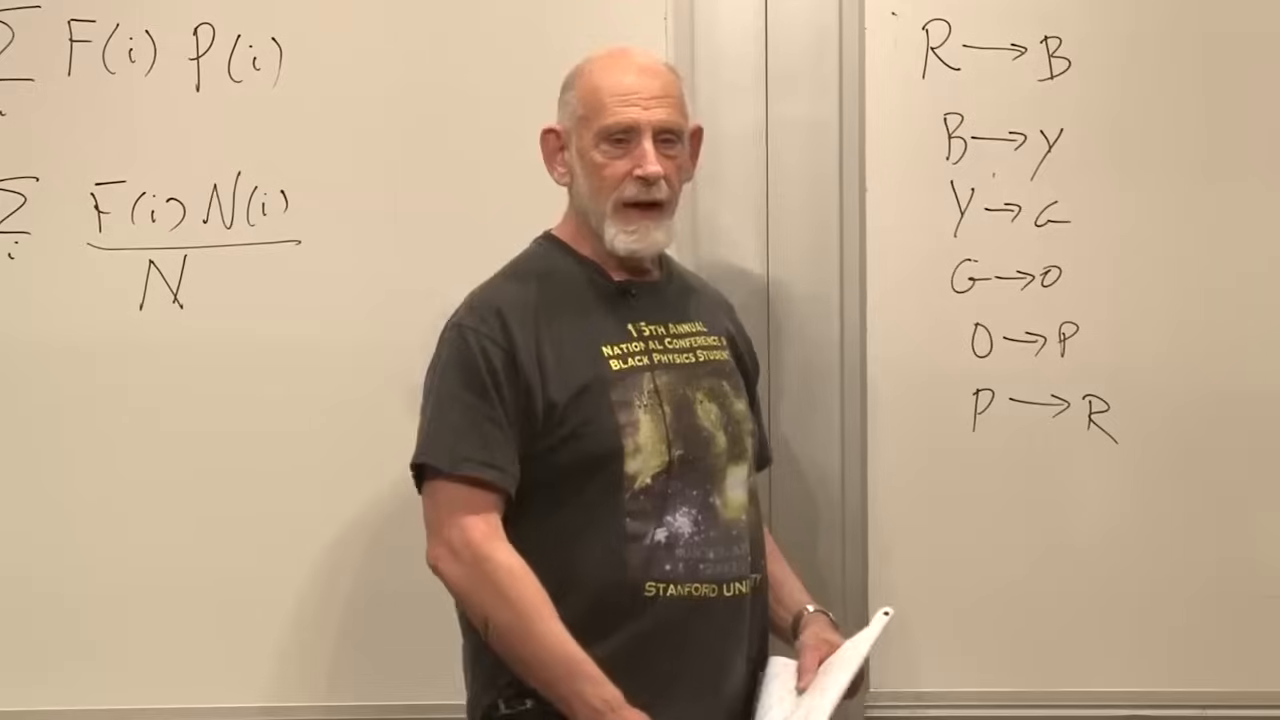
\includegraphics[width=0.92\textwidth]{lecture_01_figure_02.png}\caption{Die Erwartungswertformeln bleiben auf der linken Tafel stehen, während rechts die sechs deterministischen Farbwechsel aufgeführt sind.}\lectureframe{00:26:28}\end{figure}

Übersichtlicher lässt sich die Tafel als gerichteter Zyklus darstellen:
\begin{figure}[htbp]\centering
\begin{tikzpicture}[
  >=Latex,
  state/.style={draw,circle,minimum size=8mm,inner sep=1pt}
]
\node[state] (R) at (90:2.2) {$R$};
\node[state] (B) at (30:2.2) {$B$};
\node[state] (Y) at (-30:2.2) {$Y$};
\node[state] (G) at (-90:2.2) {$G$};
\node[state] (O) at (-150:2.2) {$O$};
\node[state] (P) at (150:2.2) {$P$};
\draw[->] (R) -- (B);
\draw[->] (B) -- (Y);
\draw[->] (Y) -- (G);
\draw[->] (G) -- (O);
\draw[->] (O) -- (P);
\draw[->] (P) -- (R);
\end{tikzpicture}\caption{Ein einzelner Orbit mit sechs Zuständen. Während jeder Periode wird jeder Zustand einmal durchlaufen.}\label{fig:sm1-six-cycle}\end{figure}

Angenommen, wir kennen den Anfangszustand nicht und machen zu einem unbekannten Zeitpunkt eine Momentaufnahme. Da jeder Schritt gleich lange dauert, verbringt das System ein Sechstel einer Periode in jeder Farbe:
\begin{equation}
 p(R)=p(B)=p(Y)=p(G)=p(O)=p(P)=\frac16.
 \label{eq:sm1-uniform-cycle}
\end{equation}
Die Gleichheit folgt nicht aus der Form des Gegenstands. Sie ergibt sich daraus, dass das System gleich lange in den einzelnen Zuständen verweilt.

Wir können die Pfeile neu anordnen und so ein anderes mikroskopisches Gesetz erhalten, das weiterhin einen Zyklus mit sechs Zuständen bildet. Die genaue Abfolge ändert sich, doch die Wahrscheinlichkeit für eine Momentaufnahme bleibt \(1/6\), weil jeder Zustand weiterhin einmal pro Periode auftritt. Für diese Vorhersage brauchen wir daher weder den Startpunkt noch die genaue Reihenfolge. Es genügen die Orbitstruktur und eine gleiche Verweildauer pro Schritt.

\begin{classroomqa}\classquestion{Wenn der Gegenstand nicht symmetrisch ist, in welchem Sinn ist es dann zulässig, jeder Farbe die Wahrscheinlichkeit \(1/6\) zuzuweisen?}\lecturerresponse{Die Zuweisung ist dynamischer, nicht geometrischer Art. Eine Momentaufnahme zu einer unbekannten Phase eines Zyklus mit sechs Schritten erfasst einen von sechs gleich langen Zeitabschnitten. Gleichwertig sind dabei die Positionen auf dem Orbit, nicht die Seiten des Gegenstands. Bei ungleichen Verweildauern wären auch die Wahrscheinlichkeiten ungleich.
\lecturetimestamp{00:27:11--00:29:49}}\end{classroomqa}

\section{Getrennte Zyklen und Erhaltungsgrößen}

Ein deterministisches Gesetz muss nicht alle Zustände auf einen einzigen Orbit legen. Betrachten wir zwei getrennte Zyklen,
\begin{equation}
 R\longrightarrow B\longrightarrow G\longrightarrow R,
 \qquad
 P\longrightarrow Y\longrightarrow O\longrightarrow P.
 \label{eq:sm1-two-cycles}
\end{equation}
Wissen wir, dass das System auf dem ersten Zyklus liegt, gilt
\begin{equation}
 \begin{aligned}
 p(R)=p(B)=p(G)&=\frac13,\\
 p(P)=p(Y)=p(O)&=0.
 \end{aligned}
\end{equation}
Wissen, dass es auf dem zweiten Zyklus liegt, vertauscht diese Zuordnungen.

Im allgemeineren Fall braucht man vorgegebene Gewichte. Bezeichnen wir die Zyklen mit \(+1\) und \(-1\) und ihre Wahrscheinlichkeiten mit \(p_+\) und \(p_-\), wobei
\begin{equation}
 p_++p_-=1.
\end{equation}
Dann gilt
\begin{align}
 p(R)=p(B)=p(G)&=\frac{p_+}{3},\\
 p(P)=p(Y)=p(O)&=\frac{p_-}{3}.
 \label{eq:sm1-sector-weights}
\end{align}
Die Faktoren \(1/3\) folgen aus der Bewegung innerhalb eines Zyklus. Die Zahlen \(p_+\) und \(p_-\) tun das nicht. Sie müssen aus zusätzlichen Informationen stammen, vielleicht aus einem weiteren Experiment oder einem anderen System, das den Anfangssektor auswählt.

Die Bezeichnungen \(+1\) und \(-1\) definieren eine Erhaltungsgröße: Beginnt das System auf einem Zyklus, führt das Aktualisierungsgesetz es niemals auf den anderen. Man kann die Größe Energie nennen oder ihr einen Platzhalternamen wie \emph{Nullgröße} geben. Ihr Name ist zweitrangig. Erhaltung bedeutet, dass der Zustandsraum in Bereiche aufgeteilt ist, die die Dynamik nicht überschreiten kann.

Die Zyklen müssen nicht gleich viele Zustände enthalten. Auch ein Orbit mit vier Zuständen und einer mit zwei Zuständen bilden zwei erhaltene Sektoren. Die Gleichzeitstichprobe ergibt dann innerhalb des ersten \(1/4\) und innerhalb des zweiten \(1/2\), jeweils multipliziert mit der vorgegebenen Wahrscheinlichkeit des betreffenden Sektors. Die statistische Mechanik muss zwei logisch getrennte Fragen beantworten:
\begin{enumerate}\item Wie viel Zeit verbringt die Dynamik, gegeben einen erhaltenen Sektor, in dessen Zuständen?
\item Welche Wahrscheinlichkeit ist dem erhaltenen Sektor selbst zuzuweisen?
\end{enumerate}

\begin{classroomqa}\audiencequestion{Nehmen wir an, dass alle Zustände innerhalb eines erhaltenen Sektors dieselbe Wahrscheinlichkeit erhalten?}\lecturerresponse{Für die hier gezeigten diskreten Spielzeuggesetze: ja, denn jeder Zustand dauert gleich lang und die Bewegung ist deterministisch. Unbekannt ist die Anfangsphase des Orbits. Ein Detektor mit Millisekunden-Auflösung kann Aktualisierungen im Mikrosekundenbereich nicht auflösen, doch eine hinreichend schnelle Momentaufnahme kann den erfassten Zustand weiterhin bestimmen. In einem allgemeineren System müssen ungleiche Verweildauern ausdrücklich berücksichtigt werden.
\lecturetimestamp{00:36:16--00:37:17}}\end{classroomqa}

\begin{classroomqa}\audiencequestion{Wenn zwei Momentaufnahmen gemacht werden und die erste einen Zyklus identifiziert, sollte die zweite dann denselben Zyklus identifizieren?}\lecturerresponse{Ja. Genau das bedeutet Erhaltung. Sobald eine Messung den Wert der Erhaltungsgröße bestimmt, können künftige Wahrscheinlichkeiten auf diesen Wert bedingt werden; Zustände im anderen Sektor erhalten dann die Wahrscheinlichkeit null.
\lecturetimestamp{00:37:18--00:37:45}}\end{classroomqa}

\subsection{Zwischen zwei Systemen geteilte Energie}

Ersetzen wir nun die abstrakte Bezeichnung durch Energie. Ein einzelner isolierter Kasten ist ein abgeschlossenes System und hat eine erhaltene Energie. Zwei isolierte Kästen haben zwei jeweils getrennt erhaltene Energien, weil sie nicht miteinander wechselwirken. Verbindet man sie durch einen schmalen Durchgang, durch den Energie fließen kann, können sich die einzelnen Energien ändern, während die Gesamtenergie erhalten bleibt.

\begin{figure}[htbp]\centering
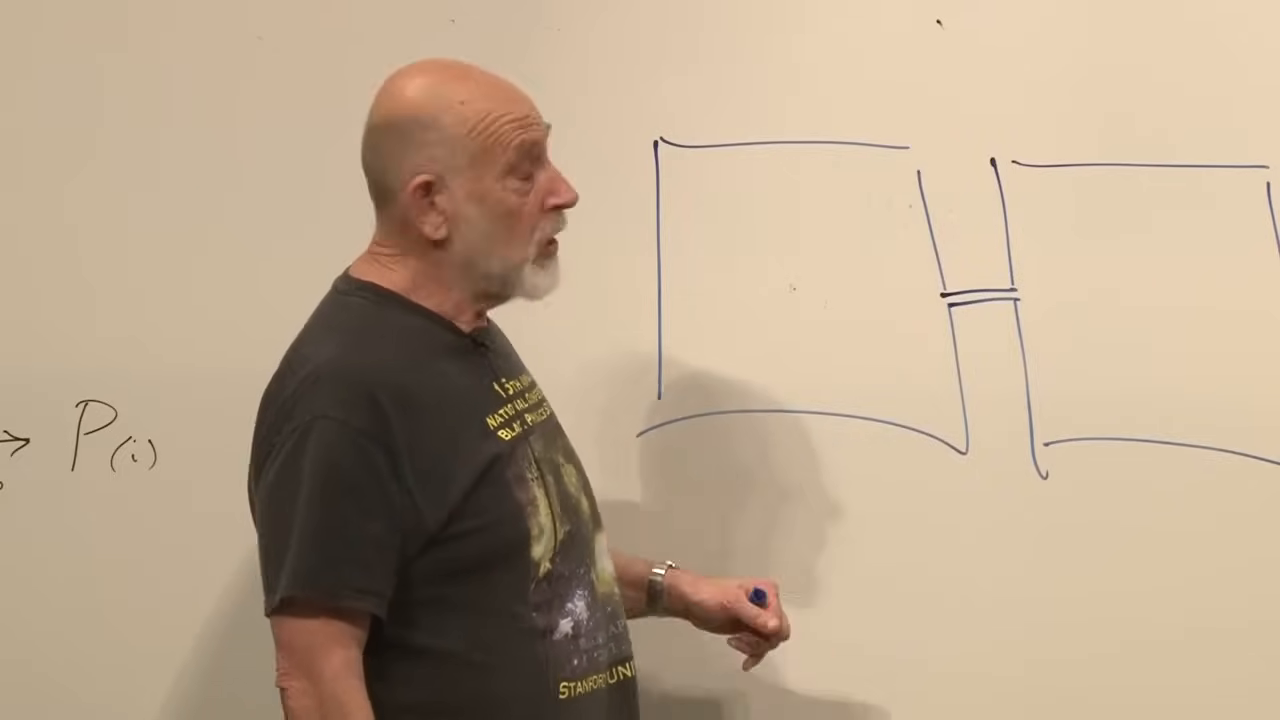
\includegraphics[width=0.92\textwidth]{lecture_01_figure_03.png}\caption{Zwei Teilsysteme, verbunden durch einen schmalen Kanal, durch den Energie fließen kann.}\lectureframe{00:39:19}\end{figure}

\begin{figure}[htbp]\centering
\begin{tikzpicture}[>=Latex]
\draw[thick,rounded corners=4pt] (-4,1.8) rectangle (-0.7,-1.5);
\draw[thick,rounded corners=4pt] (0.7,1.5) rectangle (4,-1.8);
\draw[thick] (-0.7,0.45) -- (0.7,0.45);
\draw[thick] (-0.7,-0.35) -- (0.7,-0.35);
\draw[<->,very thick] (-0.45,0.05) -- (0.45,0.05);
\node at (-2.35,0.15) {subsystem \(1\)};
\node at (2.35,-0.15) {subsystem \(2\)};
\node[above] at (0,0.5) {energy exchange};
\end{tikzpicture}\caption{Nach dem Öffnen der Verbindung ist nur noch \(E_1+E_2\) erhalten. Die Energieaufteilung wird zu einem Wahrscheinlichkeitsproblem.}\label{fig:sm1-connected-systems}\end{figure}

Bei gegebener Gesamtenergie können wir nach der Wahrscheinlichkeit fragen, dass Teilsystem \(1\) die Energie \(E_1\) hat, während Teilsystem \(2\) den Rest besitzt. Im Mittel sollten gleich große Kästen gleich viel Energie haben, doch der Mittelwert beschreibt nicht die gesamte Verteilung. Eine Möglichkeit, Wahrscheinlichkeiten für ein Teilsystem zu bestimmen, besteht daher darin, es in ein größeres abgeschlossenes System einzubetten, dessen Erhaltungssatz die fehlenden Informationen liefert. Diese Konstruktion wird in der statistischen Mechanik immer wieder auftauchen.

\section{Gute Gesetze, schlechte Gesetze und der minus erste Hauptsatz}

Nicht jede deterministische Aktualisierungsregel ist als fundamentales Gesetz zulässig. Betrachten wir die Abbildung
\begin{equation}
 \begin{aligned}
 R&\mapsto R,& B&\mapsto R,& Y&\mapsto R,\\
 G&\mapsto R,& O&\mapsto R,& P&\mapsto R.
 \end{aligned}
 \label{eq:sm1-all-to-red}
\end{equation}
Sie sagt die Zukunft perfekt voraus: Nach einem Schritt ist der Zustand rot. In umgekehrter Richtung versagt sie. Ist das System einmal rot, lässt sich nicht erkennen, ob es zuvor blau, gelb, grün, orange, violett oder ebenfalls rot war.

\begin{figure}[htbp]\centering
\begin{tikzpicture}[
  >=Latex,
  state/.style={draw,circle,minimum size=8mm,inner sep=1pt}
]
\node[state,fill=red!12] (R) at (0,0) {$R$};
\node[state] (B) at (-3,1.6) {$B$};
\node[state] (Y) at (-3,0) {$Y$};
\node[state] (G) at (-3,-1.6) {$G$};
\node[state] (O) at (3,1.6) {$O$};
\node[state] (P) at (3,-1.6) {$P$};
\draw[->] (B) -- (R);
\draw[->] (Y) -- (R);
\draw[->] (G) -- (R);
\draw[->] (O) -- (R);
\draw[->] (P) -- (R);
\draw[->,loop above] (R) to (R);
\end{tikzpicture}\caption{Ein Gesetz, das viele Zustände auf einen abbildet, sagt den nächsten Zustand voraus, löscht aber die Unterscheidungen zwischen möglichen früheren Zuständen aus.}\label{fig:sm1-bad-law}\end{figure}

Ein geschlossener Zyklus bewahrt dagegen die Aufzeichnung. Ist die verstrichene Zeit bekannt, können wir den Zustand vorwärts oder rückwärts entwickeln, selbst nach vielen Tausend Perioden. Das Gesetz erhält die Unterscheidbarkeit der Anfangsbedingungen. Susskind nennt diese Forderung den \emph{minus ersten Hauptsatz der Physik}: Information geht nicht grundlegend verloren.

Für einen endlichen diskreten Zustandsraum ist das Kriterium im Diagramm einfach:
\begin{quote}
Von jedem Zustand eines guten Gesetzes geht genau ein Pfeil aus, und genau ein Pfeil führt in ihn hinein.
\end{quote}
Der ausgehende Pfeil bestimmt die Zukunft; der eingehende rekonstruiert die Vergangenheit. Mathematisch ist die Aktualisierung eine Permutation der Zustände.

\subsection{Reibung ist nur ein scheinbares Gegenbeispiel}

Das kontinuierliche Gegenstück ist der Satz von Liouville. Reibung scheint ihm zu widersprechen. Schiebt man einen Radiergummi über einen Tisch, kommt er unabhängig davon, wo er startet, schließlich zur Ruhe. Eine schematische Gleichung für den Widerstand lautet
\begin{equation}
 m\ddot x=-\gamma\dot x,
 \qquad \gamma>0.
 \label{eq:sm1-drag}
\end{equation}
Seine Geschwindigkeit nimmt exponentiell ab. Wäre dies das fundamentalste Gesetz für jedes Teilchen in einem versiegelten Raum, käme alle Bewegung zum Erliegen, die Temperatur sänke auf null, und viele Anfangszustände würden zu einem einzigen Endzustand zusammenfallen. Die Energieerhaltung wäre verletzt, Information ginge verloren und die Unordnung nähme ab. Das wäre im Kontinuum das Gegenstück dazu, dass alles rot wird.

Echte Reibung bewirkt das nicht. Der Radiergummi erwärmt den Tisch, sich selbst und die Umgebung. Mikroskopische Positionen und Impulse halten die Unterscheidungen fest, die in der sichtbaren Bewegung verloren gehen. Reibung ist eine effektive Gleichung für ein Teilsystem, nachdem unbeobachtete Freiheitsgrade ausgeblendet wurden; sie ist kein fundamentales dissipatives Gesetz für das vollständige abgeschlossene System.

\begin{classroomqa}\classquestion{Was beschreibt die Differentialgleichung \(m\ddot x=-\gamma\dot x\), und warum ist sie kein fundamentales Gesetz für ein abgeschlossenes System?}\lecturerresponse{Sie beschreibt viskosen Widerstand. Für sich genommen treibt sie jede Geschwindigkeit gegen null; damit würde ein Gas unabhängig von seiner Anfangstemperatur auf null abkühlen. In einer tatsächlichen Beschreibung eines abgeschlossenen Systems gehen die verlorene mechanische Energie und Information in mikroskopische Freiheitsgrade über. Die Widerstandsgleichung ist nur dann verlässlich, wenn diese Variablen unterdrückt wurden.
\lecturetimestamp{00:44:40--00:48:56}}\end{classroomqa}

\section{Besetzte Zustände und die erste Entropie}

Die Erhaltung der Information hat eine entsprechende probabilistische Aussage. Angenommen, \(M\) von \(N\) Zuständen wird jeweils dieselbe Wahrscheinlichkeit zugewiesen:
\begin{equation}
 p_i=
 \begin{cases}
 1/M, & i\text{ in the occupied set},\\
 0, & i\text{ outside it}.
 \end{cases}
 \label{eq:sm1-uniform-occupied}
\end{equation}
Eine informationsbewahrende Aktualisierung kann die besetzten Zustände neu verteilen, aber sie kann sie nicht zusammenführen. Zu jedem späteren Zeitpunkt gibt es weiterhin \(M\) Zustände mit der Wahrscheinlichkeit \(1/M\). Die schlechte Abbildung \eqref{eq:sm1-all-to-red} kann dagegen viele besetzte Zustände zu einem einzigen zusammenfallen lassen.

Die Zahl \(M\) misst Unwissenheit. Wenn \(M=N\) gilt, ist jeder Zustand möglich und unsere Unwissenheit maximal. Wenn \(M=1\) gilt, ist der mikroskopische Zustand genau bekannt. Die erste Definition der Entropie lautet daher
\begin{equation}
 S=\log M.
 \label{eq:sm1-entropy-logm}
\end{equation}
Damit ergibt sich
\begin{equation}
 S_{\max}=\log N,
 \qquad
 S_{\min}=0.
\end{equation}
Ist der Zustandsraum unendlich, muss es keine endliche obere Schranke geben.

In dieser Darstellung tritt die Entropie vor der Temperatur auf, sogar vor der formalen Formulierung der Energieerhaltung. In diesem Sinn ist sie grundlegender. Sie ist jedoch keine Eigenschaft des mechanischen Systems allein. Sie hängt sowohl vom System als auch von der Wahrscheinlichkeitsverteilung ab, die das bekannte Wissen repräsentiert. Verschiedene Beobachter mit unterschiedlichem Wissen können demselben mechanischen System unterschiedliche Entropien zuweisen.

Bei exakter mikroskopischer Entwicklung werden die besetzten Zustände lediglich neu angeordnet; diese feinkörnige Entropie bleibt also erhalten. In der Praxis verlieren wir die zeitliche Auflösung, verwerfen Korrelationen und können die enorm vielen Variablen nicht verfolgen. Unsere Wahrscheinlichkeitsverteilung erstreckt sich dann über mehr Alternativen, und die der grobkörnigen Beschreibung zugewiesene Entropie nimmt zu. Die Gleichungen müssen Information nicht zerstören, damit unsere brauchbare Beschreibung sie verliert.

\begin{classroomqa}\classquestion{Wie groß ist die maximal mögliche Entropie eines endlichen Systems mit \(N\) Zuständen?}\lecturerresponse{Sie beträgt \(\log N\) und wird erreicht, wenn alle \(N\) Zustände gleich wahrscheinlich sind. Die minimale Entropie ist null und wird erreicht, wenn ein Zustand die Wahrscheinlichkeit eins hat. Entropie misst somit sowohl den Wissensstand als auch den verfügbaren Zustandsraum.
\lecturetimestamp{00:56:46--00:58:19}}\end{classroomqa}

\section{Liouville-Fluss im kontinuierlichen Phasenraum}

Bei Teilchen mit kontinuierlichen Positionen und Impulsen entspricht ein mikroskopischer Zustand einem Punkt im Phasenraum. Die Koordinaten schreiben wir als \(q_a\) und die zugehörigen konjugierten Impulse als \(p_a\). Bei vielen Teilchen gibt es sehr viele Achsen; eine zweidimensionale Zeichnung mit einem \(q\) und einem \(p\) ist nur ein Ersatzbild. Der Phasenraum ist geradzahligdimensional, weil zu jeder Koordinate ein Impuls gehört.

Angenommen, unser Wissen wird durch ein Gebiet \(\Omega_0\) dargestellt: Die Wahrscheinlichkeitsdichte ist innerhalb des Gebiets gleichmäßig und außerhalb null. Wenn wir etwa wissen, dass sich jedes Teilchen im Raum befindet, sind die Positionskoordinaten eingeschränkt; Begrenzungen der Geschwindigkeiten schränken die Impulskoordinaten ein.

Die Hamiltonsche Entwicklung führt jeden Phasenraumpunkt entlang einer Bahn. Benachbarte Punkte bewegen sich zu benachbarten Punkten, und das besetzte Gebiet entwickelt sich wie ein Teilchenvolumen einer inkompressiblen Flüssigkeit:
\begin{figure}[htbp]\centering
\begin{tikzpicture}[>=Latex,scale=0.95]
\draw[->] (-4.2,0) -- (4.3,0) node[right] {$q$};
\draw[->] (-3.7,-2.2) -- (-3.7,2.4) node[above] {$p$};
\draw[fill=blue!12,thick]
  (-3.0,-0.5) .. controls (-2.7,1.0) and (-1.3,1.2) .. (-0.9,0.1)
  .. controls (-0.6,-1.0) and (-2.2,-1.4) .. cycle;
\node at (-1.9,0.0) {$\Omega_0$};
\draw[->,very thick] (-0.3,0.2) -- (0.8,0.2);
\draw[fill=orange!15,thick]
  (1.2,-1.1) .. controls (1.5,0.3) and (2.3,1.8) .. (3.2,1.1)
  .. controls (3.6,0.7) and (2.8,-0.4) .. (2.5,-1.5)
  .. controls (2.1,-1.8) and (1.5,-1.6) .. cycle;
\node at (2.35,0.1) {$\Omega_t$};
\end{tikzpicture}\caption{Der Hamiltonsche Fluss kann ein besetztes Phasenraumgebiet strecken und scheren, erhält aber sein Volumen.}\label{fig:sm1-liouville-flow}\end{figure}

Der Satz von Liouville besagt
\begin{equation}
 \operatorname{Vol}(\Omega_t)
 =
 \operatorname{Vol}(\Omega_0).
 \label{eq:sm1-liouville-volume}
\end{equation}
Ist die Anfangsdichte auf \(\Omega_0\) gleichmäßig, so ist die transportierte Dichte auf \(\Omega_t\) ebenfalls gleichmäßig. Dies ist das kontinuierliche Gegenstück dazu, Anzahl und Gewichte besetzter diskreter Zustände zu erhalten.

Der Satz löst auch das Rätsel der Reibung auf geometrische Weise. Betrachtet man nur den sichtbaren Impuls des Radiergummis, scheint sich eine Wolke möglicher Zustände auf \(p=0\) zusammenzuziehen. Im vollständigen Phasenraum breitet sich die Wolke in die Positionen und Impulse der Moleküle im Radiergummi und im Tisch aus. Eine Projektion kann sich zusammenziehen, während das Volumen im vollständigen hochdimensionalen Raum konstant bleibt.

\begin{classroomqa}\classquestion{Wenn sich jede sichtbare Bahn der Ruhe nähert, ist dann das besetzte Phasenraumgebiet auf die Achse \(p=0\) zusammengeschrumpft?}\lecturerresponse{Nur in der reduzierten Projektion. Das vollständige System umfasst die mikroskopischen Variablen des Tisches, des Radiergummis und der Umgebung. Während sich der Bereich sichtbarer Impulse verengt, breitet sich die Verteilung in diesen verborgenen Richtungen aus. Der Satz von Liouville gilt für den vollständigen Phasenraum des abgeschlossenen Systems, nicht für eine unvollständige Menge makroskopischer Variablen.
\lecturetimestamp{01:04:37--01:06:29}}\end{classroomqa}

\section{Vom minus ersten Hauptsatz zum ersten Hauptsatz}

\subsection{Ein kurzer Blick auf den nullten Hauptsatz}

Bevor wir den ersten Hauptsatz formulieren, ist es hilfreich, den nullten zu benennen. Thermisches Gleichgewicht ist noch nicht definiert; vorerst ist der Hauptsatz daher nur eine strukturelle Aussage:
\begin{quote}
Befindet sich System \(A\) mit \(B\) im thermischen Gleichgewicht und \(B\) mit \(C\) im thermischen Gleichgewicht, so befindet sich \(A\) mit \(C\) im thermischen Gleichgewicht.
\end{quote}
Diese Transitivität wird später die Temperatur möglich machen. Für den Augenblick stellen wir sie zurück.

\subsection{Energieerhaltung}

Der erste Hauptsatz für ein abgeschlossenes System lautet schlicht
\begin{equation}
 \frac{dE}{dt}=0.
 \label{eq:sm1-first-law}
\end{equation}
In seiner knappen Form steckt große Aussagekraft. Energie ist eine Erhaltungsgröße, und der Begriff Energie wird später noch thermodynamisch angereichert.

Besteht ein abgeschlossenes System aus zwei Teilen und sind ihre Energien additiv,
\begin{equation}
 E=E_1+E_2,
\end{equation}
so gilt
\begin{equation}
 \frac{dE_1}{dt}+\frac{dE_2}{dt}=0,
 \qquad\text{or}\qquad
 \frac{dE_1}{dt}=-\frac{dE_2}{dt}.
 \label{eq:sm1-energy-exchange}
\end{equation}
Die zweite Form macht den Austausch ausdrücklich: Was ein Teilsystem an Energie verliert, gewinnt das andere.

Die Additivitätsannahme erfordert Sorgfalt. Zwei gravitative Teilchen haben jeweils eine kinetische Energie, doch ihre Wechselwirkung trägt eine potenzielle Energie bei, die zum Paar gehört. Die Gesamtenergie bleibt erhalten, obwohl sie sich nicht exakt als Energie des einen Körpers plus Energie des anderen schreiben lässt.

In der Thermodynamik ist eine ausgezeichnete additive Näherung oft zulässig, weil die Volumenenergie mit dem Volumen wächst, während die Wechselwirkungsenergie zwischen großen benachbarten Teilen mit kurzer Reichweite hauptsächlich mit ihrer Kontaktfläche skaliert. Teilen wir einen großen Tisch in Blöcke auf: Die innere Energie jedes Blocks ist ein Volumeneffekt, die Kopplung benachbarter Blöcke ein Oberflächeneffekt. Bei großen Blöcken ist Letzterer vergleichsweise klein. Gleichung \eqref{eq:sm1-first-law} gilt exakt für das abgeschlossene Ganze; die Form für Teilsysteme \eqref{eq:sm1-energy-exchange} setzt eine vernachlässigbare Wechselwirkungsenergie voraus.

\begin{classroomqa}\audiencequestion{Setzt die Normierung \(\sum_i p_i=1\) ebenfalls voraus, dass sich die aufgeführten Ergebnisse gegenseitig ausschließen?}\lecturerresponse{Ja. Eine Zustandsbezeichnung ist so definiert, dass sich die Alternativen nicht überschneiden: Befindet sich der Würfel im gelben Zustand, so ist er nicht zugleich im roten Zustand. Im alltäglichen Sprachgebrauch können Farben gemischt sein, doch die für die Wahrscheinlichkeitsrechnung verwendete Zustandseinteilung muss aus einander ausschließenden Alternativen bestehen.
\lecturetimestamp{01:12:14--01:12:55}}\end{classroomqa}

\section{Zurück zur Entropie}

Die Vorlesung wendet sich nun ausdrücklich dem noch offenen Thema zu. Obwohl uns die Temperatur aus der Sinneserfahrung vertraut ist, handelt es sich um eine abgeleitete Größe. Entropie und Energie müssen feststehen, bevor sich die Temperatur sauber definieren lässt.

\subsection{Allgemeine Wahrscheinlichkeitsverteilungen}

Die spezielle Definition \(S=\log M\) gilt, wenn \(M\) Zustände gleich wahrscheinlich sind und alle übrigen die Wahrscheinlichkeit null haben. Eine allgemeine Verteilung muss nicht rechteckig sein. Ihre Gewichte können sich über die Zustandsbezeichnungen hinweg stetig oder unregelmäßig ändern.

\begin{figure}[htbp]\centering
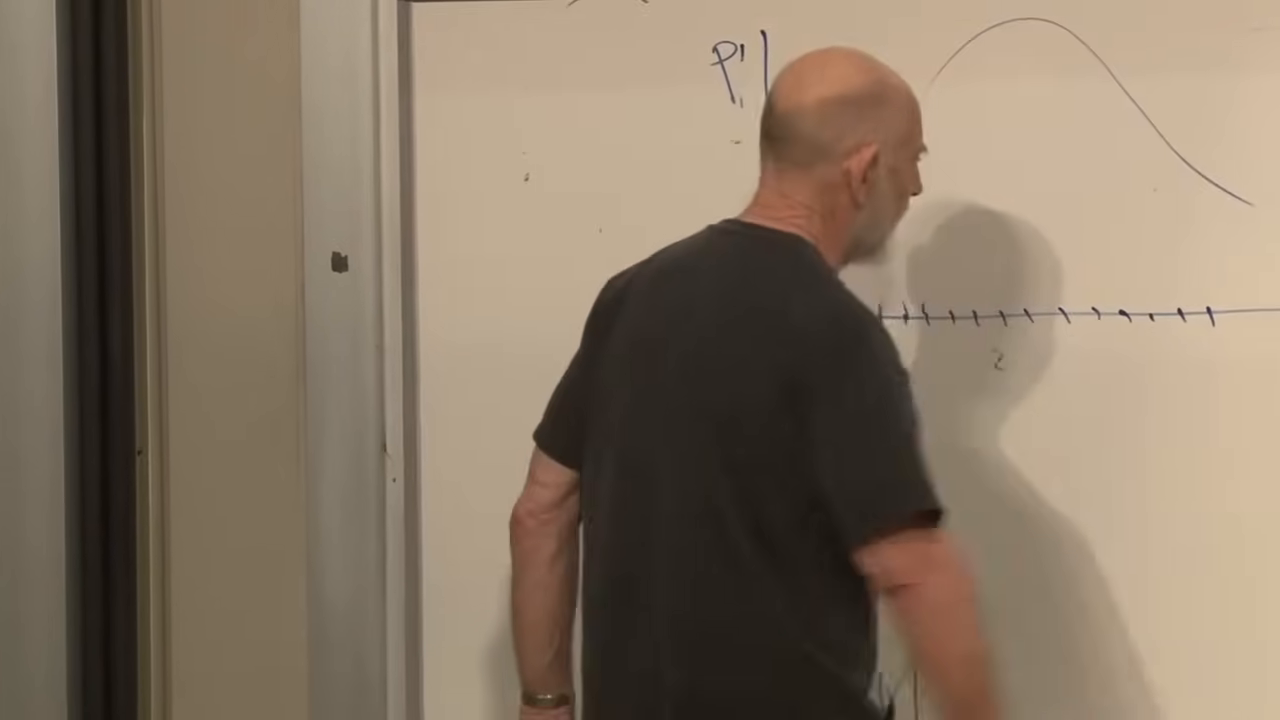
\includegraphics[width=0.92\textwidth]{lecture_01_figure_05.png}\caption{Eine Wahrscheinlichkeitsverteilung über diskreten Zustandsbezeichnungen. Für die Entropie ist die Breite der Verteilung entscheidend, nicht der genaue Kurvenverlauf.}\lectureframe{01:14:40}\end{figure}

\begin{figure}[htbp]\centering
\resizebox{\linewidth}{!}{%
\begin{tikzpicture}[>=Latex,scale=0.93]
\draw[->] (-4.2,0) -- (4.4,0) node[right] {state label \(i\)};
\draw[->] (-4,0) -- (-4,3.2) node[above] {$p_i$};
\foreach \x in {-3.6,-3.1,...,3.6}
  \draw (\x,0.08) -- (\x,-0.08);
\draw[very thick]
  plot[smooth] coordinates {
  (-3.7,0.12) (-3.0,0.28) (-2.3,0.72) (-1.6,1.45)
  (-0.9,2.25) (-0.2,2.65) (0.5,2.28) (1.2,1.55)
  (1.9,0.88) (2.7,0.38) (3.5,0.14)};
\draw (-1.8,-0.18) -- (-1.8,-0.5);
\draw (1.8,-0.18) -- (1.8,-0.5);
\draw[<->] (-1.8,-0.46) -- (1.8,-0.46);
\node at (0,-0.82) {effective spread};
\end{tikzpicture}}\caption{Eine schmale Verteilung bedeutet weniger Ungewissheit als eine breite. Die Entropie muss die Verteilung als Ganzes erfassen.}\label{fig:sm1-probability-spread}\end{figure}

Die allgemeine Definition lautet
\begin{equation}
 S=-\sum_i p_i\log p_i.
 \label{eq:sm1-shannon-entropy}
\end{equation}
Mit \eqref{eq:sm1-expectation} ergibt sich
\begin{equation}
 S=-\langle\log p\rangle.
\end{equation}
Das Minuszeichen gleicht aus, dass \(\log p_i<0\) gilt, wenn \(0<p_i<1\) gilt.

\subsection{Wiedergewinnung des Ergebnisses für die Gleichverteilung}

Wir müssen prüfen, ob die allgemeine Formel die erste Definition reproduziert.
Für einen unbesetzten Zustand gilt \(p_i=0\), während \(\log p_i\) divergiert. Das Produkt
hat den wohldefinierten Grenzwert
\begin{equation}
 \lim_{p\to0^+}p\log p=0.
 \label{eq:sm1-plogp-limit}
\end{equation}
Zustände mit Wahrscheinlichkeit null tragen also nichts bei.

\begin{classroomqa}
\audiencequestion{Wenn \(p_i=0\) gilt, verschwindet der Term dann wirklich? Der Logarithmus
von null ist minus unendlich.}
\lecturerresponse{Der Term wird durch den Grenzwert
\(\lim_{p\to0^+}p\log p\) definiert, der null ist. Der Faktor \(p\) geht schneller gegen null,
als der Logarithmus divergiert. Daher leisten beliebig unwahrscheinliche Zustände
beliebig kleine Beiträge, und ein exakt unmöglicher Zustand trägt nichts bei.
\lecturetimestamp{01:18:27--01:19:46}}
\end{classroomqa}

Für jeden der \(M\) besetzten Zustände gilt \(p_i=1/M\). Daher
\begin{align}
 S
 &=-\sum_{\mathrm{occupied}\ i}
 \frac1M\log\!\left(\frac1M\right)\\
 &=-M\frac1M\log\!\left(\frac1M\right)\\
 &=-\log\!\left(\frac1M\right)
 =\log M.
 \label{eq:sm1-entropy-check}
\end{align}
Der allgemeine Ausdruck stimmt exakt mit dem Spezialfall überein. Eine breitere
Verteilung gewichtet mehr Alternativen merklich und hat deshalb eine größere
Entropie; eine schmalere Verteilung hat eine kleinere Entropie.

\begin{figure}[htbp]
\centering
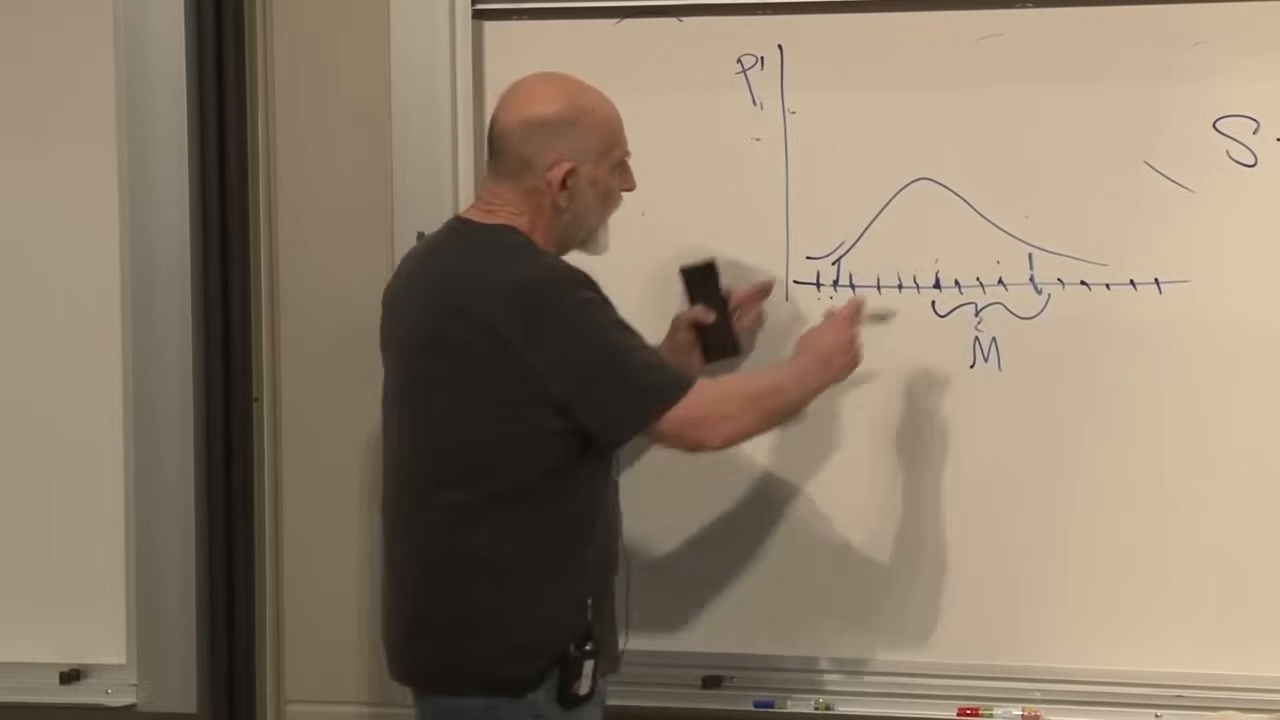
\includegraphics[width=0.92\textwidth]{lecture_01_figure_06.png}
\caption{Die markierte Breite \(M\) hebt den Zusammenhang zwischen der Streuung
der maßgeblichen Wahrscheinlichkeiten und der Entropie hervor.}
\lectureframe{01:16:42}
\end{figure}

Entropie ist einer Wahrscheinlichkeitsverteilung auf dem Zustandsraum zugeordnet. Sie ist
keine bloße Observable wie die Energie oder der Impuls eines einzelnen Mikrozustands. Ein exakter
Zustand lässt sich durch eine auf diesen Zustand konzentrierte Verteilung darstellen und
hat dann Entropie null; die Entropie ändert sich jedoch, wenn sich der Kenntnisstand
ändert.

\section{Münzen, Bits und explizites Abzählen}

Sei \(n\) die Anzahl der Münzen. Die Anzahl der mikroskopischen Konfigurationen ist
\begin{equation}
 N=2^n.
 \label{eq:sm1-coin-state-count}
\end{equation}
Wenn über die Münzen nichts bekannt ist, sind alle \(2^n\) Konfigurationen gleich
wahrscheinlich, und es gilt
\begin{equation}
 S_{\max}=\log(2^n)=n\log2.
 \label{eq:sm1-coin-max-entropy}
\end{equation}
Die Entropie ist additiv bezüglich der Anzahl unabhängiger Münzen.

Bei Logarithmen zur Basis \(2\) hat ein vollständig unbekanntes Zweizustandssystem
eine Entropie von einem Bit. Mit natürlichen Logarithmen beträgt sie \(\log2\). Die Einheit
ist Konvention; die zugrunde liegende Ordnung und Additivität bleiben unverändert.

Am anderen Extrem gilt: Wenn jede Münze bekannt ist, hat genau eine Konfiguration
die Wahrscheinlichkeit eins:
\begin{equation}
 S=0.
\end{equation}
Mehr Wissen bedeutet weniger Entropie.

Nehmen wir nun an, dass genau eine der \(n\) Münzen Zahl zeigt, alle übrigen Kopf,
und die Position der Münze mit Zahl unbekannt ist. Es gibt \(n\) gleich wahrscheinliche
Konfigurationen, eine für jede mögliche Position dieser Münze, also gilt
\begin{equation}
 S=\log n.
 \label{eq:sm1-one-tail-entropy}
\end{equation}
Dies ist im Allgemeinen kein ganzzahliges Vielfaches von \(\log2\). Ein Bit ist eine praktische
Einheit und bedeutet nicht, dass jede Entropie nur in ganzen Bits auftreten kann.

\begin{classroomqa}
\audiencequestion{Tritt \(\log2\) nur deshalb auf, weil jede Münze zwei
mögliche Zustände hat? Ergäbe ein Element mit drei Zuständen \(\log3\)?}
\lecturerresponse{Genau. Ein vollständig unbekanntes Element mit \(k\) möglichen
Zuständen trägt \(\log k\) bei. Binäre Schalter sind in Computern besonders praktisch,
weil physische Schalter sich auf natürliche Weise in zwei stabile Zustände bringen lassen
und weil zwei die kleinste nichttriviale ganze Zahl ist.
\lecturetimestamp{01:29:55--01:30:48}}
\end{classroomqa}

\begin{classroomqa}
\audiencequestion{Welche Basis ist für den Logarithmus gemeint?}
\lecturerresponse{In diesen physikalischen Formeln bezeichnet \(\log\) den natürlichen
Logarithmus. Informationstheoretiker verwenden häufig die Basis \(2\), sodass die Entropie
direkt in Bits gemessen wird. Ein Wechsel der Basis multipliziert jede Entropie mit demselben
Umrechnungsfaktor und ändert keine physikalische Schlussfolgerung.
\lecturetimestamp{01:30:49--01:32:06}}
\end{classroomqa}

\section{Entropie im kontinuierlichen Phasenraum}

Kehren wir zu einem klassischen Phasenraum \(\Gamma\) zurück. Ist die Wahrscheinlichkeitsdichte
in einem Gebiet mit Volumen \(V_\Gamma\) gleichförmig und außerhalb davon null, so lautet das
Analogon zum Abzählen von \(M\) gleich wahrscheinlichen Zuständen
\begin{equation}
 S=\log\!\left(\frac{V_\Gamma}{V_0}\right).
 \label{eq:sm1-continuous-uniform}
\end{equation}
Dabei ist \(V_\Gamma\) das Volumen im vollständigen hochdimensionalen Raum der Koordinaten
und Impulse, nicht das gewöhnliche räumliche Volumen. Das feste Volumen \(V_0\) ist eine
Referenzzelle im Phasenraum, durch die der Logarithmus dimensionslos wird. Setzt man
\(V_0=1\), erhält man die an der Tafel verwendete Kurzform \(S=\log V_\Gamma\).

Für eine allgemeine Wahrscheinlichkeitsdichte \(P(q,p)\) wird die diskrete Summe durch ein
Phasenraumintegral ersetzt. Die Normierung lautet
\begin{equation}
 \int_\Gamma d\Gamma\,P(q,p)=1,
 \label{eq:sm1-continuous-normalization}
\end{equation}
und die Entropie ist
\begin{equation}
 S=-\int_\Gamma d\Gamma\,
 P(q,p)\log\!\bigl[P(q,p)V_0\bigr].
 \label{eq:sm1-continuous-entropy}
\end{equation}
Die Dichte ist die Wahrscheinlichkeit pro Phasenraumzelle. Begrifflich misst
\eqref{eq:sm1-continuous-entropy} weiterhin, wie breit die Wahrscheinlichkeit
verteilt ist; für einen gleichförmigen Fleck ergibt sich daraus der Logarithmus des
besetzten Volumens, gemessen in Einheiten der Referenzzelle. Eine Änderung dieser festen
Zelle verschiebt jede kontinuierliche Entropie um dieselbe additive Konstante und lässt
Entropiedifferenzen unverändert.

\begin{classroomqa}
\audiencequestion{Warum hat sich das Koordinatensymbol von \(x\) zu \(q\) geändert?}
\lecturerresponse{Physikalisch ändert sich dadurch nichts. In der klassischen Mechanik
verwendet man für Koordinaten häufig entweder \(x\) oder \(q\) und für konjugierte Impulse
\(p\). Der Wechsel der Notation war lediglich ein Versehen; die Konstruktion des Phasenraums
ist dieselbe.
\lecturetimestamp{01:37:10--01:37:39}}
\end{classroomqa}

Temperatur und die Boltzmann-Verteilung werden bewusst auf später verschoben. Als Nächstes
werden wir das thermische Gleichgewicht definieren und anschließend seine
Wahrscheinlichkeitsverteilung bestimmen.

\section{Fragen zu Korrelation, Additivität und Information}

\subsection{Korrelation bedeutet, dass eine Messung die Verteilung einer anderen Größe verändert}

Bei vollständiger Unkenntnis über unabhängige Münzen wird jeder Konfiguration dieselbe
Wahrscheinlichkeit zugewiesen. Eine Messung an einer Münze verrät dann nichts über irgendeine
andere Münze. Deren Verteilungen bleiben unverändert.

Das Ensemble mit genau einer Münze, die Zahl zeigt, ist anders. Misst man bei einer Münze Zahl,
zeigt jede andere mit Sicherheit Kopf. Zeigt die gemessene Münze Kopf, muss die einzige Münze mit Zahl
unter den verbleibenden \(n-1\) Münzen sein; daher hat jede verbleibende Position die bedingte Wahrscheinlichkeit
\begin{equation}
\begin{aligned}
 p(&\text{tail at a specified remaining position}\\
   &\mid\text{measured head})=\frac{1}{n-1}.
\end{aligned}
 \label{eq:sm1-conditional-tail}
\end{equation}
Das ist Korrelation: Wenn man eine Variable kennt, ändert sich die der anderen zugewiesene
Wahrscheinlichkeitsverteilung.

\begin{classroomqa}
\audiencequestion{Wurde in den Entropiebeispielen Unabhängigkeit der Münzen vorausgesetzt?}
\lecturerresponse{Nur wenn vollständige Unkenntnis durch gleiche
Wahrscheinlichkeiten für alle \(2^n\) Konfigurationen dargestellt wurde. In diesem Fall lässt eine Messung an einer
Münze die Verteilungen der übrigen unverändert. Das Beispiel mit genau einer Münze, die Zahl zeigt,
ist ausdrücklich korreliert: Eine Messung aktualisiert, was an anderer Stelle möglich ist.
Die angegebene Information bestimmt, welche Wahrscheinlichkeitsverteilung verwendet wird.
\lecturetimestamp{01:38:43--01:41:58}}
\end{classroomqa}

Das Beispiel mit den getrennten Zyklen hat dieselbe logische Struktur. Eine Messung des erhaltenen
Labels \(+1\) oder \(-1\) beschränkt alle späteren Zustände auf einen Sektor.
Die Konditionierung auf erhaltene Information ändert die zulässige Verteilung.

Für unkorrelierte Systeme ist die Entropie additiv. Wenn
\begin{equation}
 p_{ij}=p_i^{(A)}p_j^{(B)},
\end{equation}
Dann gilt
\begin{align}
 S_{AB}
 &=-\sum_{i,j}p_i^{(A)}p_j^{(B)}
 \log\!\left[p_i^{(A)}p_j^{(B)}\right]\\
 &=S_A+S_B.
 \label{eq:sm1-entropy-additivity}
\end{align}
Korrelationen verhindern diese Faktorisierung und verringern die unabhängige
Ungewissheit des Paars.

Stell dir als Übung eine Reihe binärer Variablen vor, bei der ein Element im Zustand „oben“ dazu führt,
dass jeder Nachbar mit Wahrscheinlichkeit drei Viertel im Zustand „unten“ ist. Eine Messung an einem Ort
ändert unmittelbar, was über nahegelegene Orte bekannt ist. Eine solche Verteilung ist korreliert, und ihre
Entropie lässt sich nicht durch Addition isolierter Ein-Ort-Entropien bestimmen, ohne diese Korrelationen
zu berücksichtigen.

\subsection{Boltzmann, Shannon und die quantenmechanische Unbestimmtheit}

\begin{classroomqa}
\audiencequestion{Wie hängt die ältere thermodynamische Entropie mit der
informationstheoretischen Entropie von Shannon zusammen?}
\lecturerresponse{In beiden Fällen tritt dieselbe Funktionalform auf:
\(-\sum_i p_i\log p_i\). Shannon verwendete häufig die Basis \(2\), während Physiker
üblicherweise natürliche Logarithmen verwenden und die Boltzmann-Konstante wieder einsetzen,
wenn die Entropie in thermodynamischen Einheiten angegeben wird. Der mathematische Unterschied
besteht nur in einem festen Umrechnungsfaktor, auch wenn die physikalischen Fragen, aus denen
die Wahrscheinlichkeiten hervorgehen, sehr verschieden sein können.
\lecturetimestamp{01:44:05--01:46:06}}
\end{classroomqa}

Für gleich wahrscheinliche Mikrozustände schreibt man die thermodynamische Formel oft als
\begin{equation}
 S_{\mathrm{thermo}}=k_{\mathrm B}\log W,
 \label{eq:sm1-boltzmann-formula}
\end{equation}
Dabei ist \(W\) die Anzahl der zugänglichen Mikrozustände. In Einheiten mit
\(k_{\mathrm B}=1\) ist dies genau \(S=\log W\). Die Boltzmann-Konstante rechnet zwischen Temperatureinheiten
und Energieeinheiten um; die natürliche mikroskopische Skala der Temperatur ist die Energie.

\begin{classroomqa}
\audiencequestion{Ist diese Entropie einfach eine andere Form der Heisenbergschen
Unschärferelation?}
\lecturerresponse{Nein. Die hier betrachtete Entropie misst die Ungewissheit einer
Wahrscheinlichkeitsverteilung über mögliche Zustände. In der Quantensprache ist sie die
Ungewissheit eines gemischten Zustands, nicht die intrinsische Messunsicherheit, die auch
bei einem reinen Zustand bestehen bleiben kann. Diese beiden Begriffe müssen klar
auseinandergehalten werden.
\lecturetimestamp{01:46:07--01:47:31}}
\end{classroomqa}

\section{Was bisher gezeigt wurde}

Ausgangspunkt war nicht eine Zufälligkeit der Gesetze. Eine deterministische Dynamik erzeugt
zusammen mit unvollständiger Kenntnis des Anfangszustands bereits Wahrscheinlichkeiten. Eine einzelne
Bahn weist Zuständen Gewichte zu, je nachdem, wie viel Zeit in jedem Zustand verbracht wird; getrennte
Bahnen machen Erhaltungsgrößen sichtbar und erfordern vorherige Gewichte für die verschiedenen
Sektoren. Zulässige mikroskopische Gesetze bewahren Unterscheidungen. In einem endlichen Zustandsraum
bedeutet das, dass an jedem Zustand genau ein Pfeil ankommt und einer abgeht; in der kontinuierlichen
Mechanik entspricht dem das Liouville-Theorem.

Diese Struktur führt zunächst zu
\begin{equation}
 S=\log M
\end{equation}
für \(M\) gleich wahrscheinliche besetzte Zustände, dann zu
\begin{equation}
 S=-\sum_i p_i\log p_i,
\end{equation}
und schließlich zu seinem Phasenraumintegral. Entropie beschreibt eine Wahrscheinlichkeitsverteilung
und damit einen Kenntnisstand. Die feinkörnige Information bleibt durch das mikroskopische Gesetz
erhalten, selbst wenn eine praktische grobkörnige Beschreibung sie nicht mehr nachverfolgt.

Die Energieerhaltung liefert den ersten Hauptsatz, während die Additivität der Teilenergien eine
vernachlässigbare Wechselwirkungsenergie voraussetzt. Für die Entropie gilt eine entsprechende
Bedingung: Die Wahrscheinlichkeiten der Teilsysteme müssen unkorreliert sein. Diese beiden Arten
von Additivität bereiten den nächsten Schritt vor, bei dem thermisches Gleichgewicht, Temperatur
und die Boltzmann-Verteilung Energie mit Wahrscheinlichkeit verknüpfen.

\chapter{Temperatur aus Entropie und Energie}

\lectureoverview{Temperatur tritt zunächst als Umrechnung von Thermometereinheiten des menschlichen Maßstabs in mikroskopische Energieeinheiten auf. Nach der entsprechenden Umrechnung der thermodynamischen Entropie in dimensionslose statistische Entropie beschreiben wir das Gleichgewicht durch eine einparametrige Familie von Wahrscheinlichkeitsverteilungen. Die Ableitung \(dE/dS\) definiert dann die Temperatur, und der erste und der zweite Hauptsatz zeigen, warum eine Temperaturdifferenz die Richtung des Energieflusses bestimmt.}

\section{Umrechnungsfaktoren und menschliche Maßeinheiten}

Viele Konstanten der Physik sind Umrechnungsfaktoren. Die Lichtgeschwindigkeit rechnet eine Länge in eine Zeit um:
\begin{equation}
 t=\frac{x}{c}.
\end{equation}
Misst man Längen und Zeiten in zueinander passenden Einheiten, kann man \(c=1\) setzen. Dadurch verschwindet keine physikalische Wirkung; lediglich beide Messgrößen werden auf dieselbe Skala gebracht.

Die Boltzmann-Konstante hat denselben Charakter. Sie rechnet die auf einem Thermometer im \emph{menschlichen Maßstab} abgelesene Temperatur in eine Energie um. Der Zusatz ist wichtig. Solche Einheiten werden gewählt, weil makroskopische Instrumente sie erzeugen und auflösen können, nicht weil die mikroskopische Dynamik sie auszeichnet.

Das Grad Celsius wurde festgelegt, indem das Intervall zwischen dem Gefrier- und dem Siedepunkt von Wasser bei Normaldruck in hundert Teile geteilt wurde. Die Kelvin-Skala verwendet ein gleich großes Grad, setzt den Nullpunkt aber beim absoluten Nullpunkt an. Die Wahl eines anderen Stoffes, eines anderen Intervalls oder der Fahrenheit-Skala würde die Zahlenwerte, nicht aber die Physik verändern.

\begin{classroomqa}
\audiencequestion{War die Fahrenheit-Skala bereits eine Konstruktion des siebzehnten Jahrhunderts?}
\lecturerresponse{Das genaue Datum ist hier nicht von Bedeutung. Entscheidend ist, dass all diese Skalen für Temperaturen entworfen wurden, die Menschen erzeugen und messen konnten. Die Größe eines Grades ist eine Konvention und keine mikroskopische Vorgabe.
\lecturetimestamp{00:01:34--00:01:50}}
\end{classroomqa}

Als diese Skalen geschaffen wurden, war der molekulare Ursprung der Wärme experimentell noch nicht zugänglich. Eine Änderung um ein Grad ließ sich mit einem makroskopischen Thermometer beobachten, die Energie eines einzelnen Moleküls dagegen nicht messen. Daher lag es nahe, eine Temperatureinheit einzuführen, bevor bekannt war, dass Temperatur im Grunde eine Energieskala ist.

\section{Warum Temperatur die Einheit Energie hat}

Betrachten wir ein verdünntes einatomiges Gas. Verdünnt bedeutet hier, dass die Wechselwirkungsenergien zwischen Molekülen für den vorliegenden Zweck vernachlässigt werden können. Im thermischen Gleichgewicht ordnet das Äquipartitionstheorem jedem quadratischen translatorischen Freiheitsgrad \(T_{\mathrm K}/2\) mal die Boltzmann-Konstante zu. In drei Raumdimensionen gilt
\begin{equation}
 \left\langle E_{\mathrm{kin}}\right\rangle
 =\frac{3}{2}k_{\mathrm B}T_{\mathrm K}.
 \label{eq:sm2-equipartition-kelvin}
\end{equation}
Der Faktor drei zählt die Bewegungen in \(x\)-, \(y\)- und \(z\)-Richtung. Der Faktor ein Halb stammt aus der quadratischen kinetischen Energie.

Diese Beziehung ist nicht auf eine bestimmte Molekülsorte beschränkt. In einem Helium-Sauerstoff-Gemisch hat jedes frei translatorisch bewegliche Teilchen im Gleichgewicht dieselbe mittlere Schwerpunktskinetik, auch wenn sich die schwereren Teilchen langsamer bewegen. Da
\begin{equation}
 E_{\mathrm{kin}}=\frac{1}{2}mv^2,
\end{equation}
folgt aus gleicher charakteristischer Energie \(v\propto m^{-1/2}\).

Dieselbe Idee lässt sich auf ein bewusst extremes Beispiel übertragen. Man hänge eine Bowlingkugel in eine Flüssigkeit und lasse das gesamte System das Gleichgewicht erreichen. Für ihre Brownschen translatorischen Freiheitsgrade gilt dieselbe Energieskala wie für die eines Moleküls. Die Geschwindigkeit der Kugel ist wegen ihrer enorm viel größeren Masse unvorstellbar viel kleiner; die Temperatur vergleicht jedoch Energieskalen, nicht Geschwindigkeiten.

Bei Raumtemperatur beträgt \(T_{\mathrm K}\) etwa \(300\,\mathrm K\), während die Energie eines einzelnen mikroskopischen Freiheitsgrads in Joule winzig ist. Entsprechend klein ist der Umrechnungsfaktor:
\begin{equation}
 k_{\mathrm B}\simeq 1.38\times10^{-23}\,
 \mathrm{J\,K^{-1}}.
 \label{eq:sm2-boltzmann-value}
\end{equation}
Der Zusammenhang zwischen seiner Größenordnung und der Avogadro-Konstante ist kein Zufall:
\begin{equation}
 R=N_{\mathrm A}k_{\mathrm B}.
\end{equation}
Die Gaskonstante \(R\) beschreibt ein Mol, während \(k_{\mathrm B}\) die entsprechende Skala pro mikroskopischem Bestandteil angibt.

In grundlegenden Formeln tritt immer wieder die Kombination \(k_{\mathrm B}T_{\mathrm K}\) auf. Daher ist es übersichtlicher, \begin{equation}
 T\equiv k_{\mathrm B}T_{\mathrm K}.
 \label{eq:sm2-energy-temperature}
\end{equation} zu definieren.
Von nun an hat \(T\) selbst die Einheit einer Energie, und \eqref{eq:sm2-equipartition-kelvin} wird zu
\begin{equation}
 \left\langle E_{\mathrm{kin}}\right\rangle=\frac{3}{2}T.
 \label{eq:sm2-equipartition-natural}
\end{equation}
Misst man Energie in Joule, wird die Temperatur in Joule angegeben. Misst man Energie in Elektronenvolt, wird die Temperatur in Elektronenvolt angegeben. Es gibt keine neue Natureinheit namens Temperatureinheit.

\section{Zwei Konventionen für die Entropie}

Dieselbe Umrechnung tritt auch bei der Entropie auf. Die makroskopische Thermodynamik entwickelte sich aus der Analyse von Wärmekraftmaschinen. Carnot lieferte die entscheidenden Überlegungen zu Wärmekraftmaschinen; Clausius führte später die thermodynamische Entropie und das Symbol \(S\) ein. Bezeichnen wir diese makroskopische Größe in der hier verwendeten Notation mit \(S_{\mathrm C}\). Ihre Einheit ist Energie geteilt durch Thermometertemperatur, beispielsweise Joule pro Kelvin.

Die statistische Entropie ist dimensionslos. Für eine diskrete Verteilung gilt
\begin{equation}
 S=-\sum_i p_i\log p_i.
 \label{eq:sm2-statistical-entropy}
\end{equation}
Bei natürlichen Logarithmen hat eine gleichwahrscheinliche binäre Alternative die Entropie \(\log2\); bei Logarithmen zur Basis zwei wird derselbe Betrag als ein Bit bezeichnet. Die beiden Entropiekonventionen hängen folgendermaßen zusammen:
\begin{equation}
 S=\frac{S_{\mathrm C}}{k_{\mathrm B}},
 \qquad
 S_{\mathrm C}=k_{\mathrm B}S.
 \label{eq:sm2-entropy-conversion}
\end{equation}
Ein makroskopischer Wert, der in \(\mathrm{J\,K^{-1}}\) bescheiden erscheint, entspricht einer enormen dimensionslosen Entropie, denn diese zählt die Information, die auf eine enorme Zahl mikroskopischer Bestandteile verteilt ist.

Die Gleichungen \eqref{eq:sm2-energy-temperature} und \eqref{eq:sm2-entropy-conversion} legen die durchgehend verwendete Konvention fest:
\[
 [T]=[\text{energy}],
 \qquad
 [S]=1.
\]
Die Boltzmann-Konstante kann nun aus den Arbeitsformeln verschwinden. Sie lässt sich jederzeit wieder einsetzen, indem man \(T\) durch \(k_{\mathrm B}T_{\mathrm K}\) und \(S\) durch \(S_{\mathrm C}/k_{\mathrm B}\) ersetzt.

\begin{classroomqa}
\audiencequestion{Ist die neue Temperatur abgesehen vom Faktor \(3/2\) einfach eine in Joule gemessene Energie?}
\lecturerresponse{Ja, sofern Joule als Energieeinheit gewählt wird. Ein Joule ist die MKS-Einheit \(\mathrm{kg\,m^2\,s^{-2}}\). Man könnte stattdessen Elektronenvolt oder eine andere Energieeinheit verwenden; dann muss die Temperatur in derselben Einheit angegeben werden. Der Faktor \(3/2\) gehört zum Beispiel des idealen Gases, nicht zur Definition der Temperatur.
\lecturetimestamp{00:15:49--00:16:45}}
\end{classroomqa}

\begin{classroomqa}
\audiencequestion{Wenn die Tafel Kelvin vorgibt, ist \(k_{\mathrm B}\) dann nicht eine festgelegte Konstante?}
\lecturerresponse{Sie ist festgelegt, sobald sowohl die Temperatur- als auch die Energieeinheit angegeben sind. Wechselt man von Kelvin zu Fahrenheitgraden oder von Joule zu Elektronenvolt, ändert sich ihr Zahlenwert. Genau so muss sich ein Umrechnungsfaktor mit der Einheit ändern.
\lecturetimestamp{00:16:46--00:18:33}}
\end{classroomqa}

\begin{classroomqa}
\audiencequestion{Wird der Zahlenwert der Boltzmann-Konstante experimentell bestimmt?}
\lecturerresponse{Ja. Historisch erforderte ihre Bestimmung mikroskopische Informationen über Atome und deren Teilchendichte. Boltzmann verstand den Zusammenhang zwischen Molekülenergie und Temperatur, bevor diese Größen genau bekannt waren – ähnlich wie Newton die Rolle der Gravitationskonstante kannte, bevor sie präzise gemessen worden war.
\lecturetimestamp{00:18:46--00:20:00}}
\end{classroomqa}

\section{Gleichgewicht ist ein statistischer Zustand}

Die Einheitenumrechnung hat die Temperatur noch immer nicht definiert. Etwas Heißes zu berühren vermittelt eine nützliche biologische Intuition, doch Temperatur ist eine abgeleitete physikalische Größe, die aus Energie und Entropie gebildet wird.

Man stelle sich ein System vor, das mit einer großen Umgebung in Kontakt steht, deren makroskopische Bedingungen festgehalten werden. Energie kann zwischen beiden ausgetauscht werden. Hat das System anfangs zu viel Energie, gibt es im Mittel Energie ab; hat es zu wenig, nimmt es im Mittel Energie auf. Im thermischen Gleichgewicht finden weiterhin mikroskopische Austauschvorgänge statt, doch im Mittel gibt es keinen Nettofluss in eine der beiden Richtungen.

Bezeichne \(i\) einen exakten mikroskopischen Zustand des Systems und \(E_i\) dessen Energie. Gleichgewicht bedeutet nicht, dass das System in einem Zustand erstarrt. Seine Wechselwirkung mit der Umgebung verändert den Mikrozustand fortwährend, daher ordnen wir jeder Möglichkeit eine Wahrscheinlichkeit \(P_i\) zu. Die grundlegenden Beziehungen lauten
\begin{align}
 \sum_i P_i &=1,
 \label{eq:sm2-normalization}\\
 \sum_i P_iE_i &=\overline E,
 \label{eq:sm2-mean-energy}\\
 S&=-\sum_iP_i\log P_i.
 \label{eq:sm2-equilibrium-entropy}
\end{align}
Der Balken über \(\overline E\) hebt hervor, dass die Energie des Teilsystems schwankt. Eine Messung kann einen Wert ergeben, die nächste einen anderen; bei wiederholten Messungen ergibt sich die Verteilung, deren Mittelwert \eqref{eq:sm2-mean-energy} ist.

\begin{figure}[t]
\centering
\includegraphics[width=0.82\textwidth]{lecture_02_figure_02.png}
\caption{Normierung und mittlere Energie an der Tafel: \(\sum_iP(i)=1\) und \(\sum_iP(i)E(i)=\langle E\rangle\).}
\lectureframe{00:24:10}
\end{figure}

\section{Eine durch die mittlere Energie parametrisierte Familie}

Die Gleichgewichtsverteilung hängt stark von der mittleren Energie ab. Stellt man einen Topf Wasser auf den Herd, steigt \(\overline E\); stellt man ihn in den Schnee, sinkt \(\overline E\). Die Wahrscheinlichkeiten ändern sich entsprechend. Gleichgewicht sollte daher nicht als eine einzelne Verteilung, sondern als einparametrige Familie betrachtet werden:
\begin{equation}
 P_i(\overline E).
 \label{eq:sm2-family}
\end{equation}
Jedes Familienmitglied erfüllt
\begin{align}
 \sum_iP_i(\overline E)&=1,
 \label{eq:sm2-family-normalization}\\
 \sum_iP_i(\overline E)E_i&=\overline E.
 \label{eq:sm2-family-mean}
\end{align}

\begin{figure}[t]
\centering
\includegraphics[width=0.88\textwidth]{lecture_02_figure_03.png}
\caption{Der Übergang zu \(P(i,\overline E)\). Die vorherigen Gleichungen für Normierung, mittlere Energie und Entropie bleiben sichtbar, während die Verteilungsfamilie eingeführt wird.}
\lectureframe{00:26:29}
\end{figure}

Für eine schematische Darstellung ordnen wir die Zustände nach aufsteigendem \(E_i\). Die horizontale Achse kann dann entweder als Index \(i\) oder als zugehörige Energie gelesen werden. Bei größerer mittlerer Energie verschiebt sich das Wahrscheinlichkeitsgewicht zu weiter rechts liegenden Zuständen. Die Gesamtfläche unter jeder Kurve muss weiterhin eins betragen.

\begin{figure}[t]
\centering
\includegraphics[width=0.88\textwidth]{lecture_02_figure_04.png}
\caption{Mehrere schematische Verteilungen \(P(i,\overline E)\). Kurven, deren Gewicht weiter rechts liegt, haben eine größere mittlere Energie; jede bleibt normiert.}
\lectureframe{00:28:40}
\end{figure}

\begin{figure}[t]
\centering
\begin{tikzpicture}[x=1cm,y=1cm]
\draw[->] (0,0) -- (7.4,0) node[right] {$E_i$};
\draw[->] (0,0) -- (0,3.25) node[above] {$P_i(\overline E)$};
\draw[thick,blue!70!black]
  plot[smooth] coordinates {(0,0) (0.35,1.6) (0.85,2.65) (1.45,1.45)
  (2.2,0.35) (3.0,0)};
\draw[thick,teal!70!black]
  plot[smooth] coordinates {(0,0) (0.7,0.7) (1.5,1.7) (2.5,2.0)
  (3.7,0.8) (4.8,0)};
\draw[thick,orange!80!black]
  plot[smooth] coordinates {(0,0) (1.3,0.3) (2.7,0.9) (4.3,1.45)
  (5.8,0.85) (7.0,0)};
\node[blue!70!black] at (1.0,2.95) {\(\overline E_1\)};
\node[teal!70!black] at (2.75,2.3) {\(\overline E_2\)};
\node[orange!80!black] at (5.2,1.7) {\(\overline E_3\)};
\node at (4.9,2.85) {\(\overline E_1<\overline E_2<\overline E_3\)};
\end{tikzpicture}
\caption{Eine bereinigte Fassung der Skizze an der Tafel. Die Kurven müssen nicht genau diese Formen haben; berücksichtigt werden lediglich die Normierung und die aufsteigend geordneten mittleren Energien.}
\end{figure}

\begin{classroomqa}
\audiencequestion{Ist die Notation zirkulär? Die mittlere Energie wird aus der Verteilung berechnet, während die Verteilung durch die mittlere Energie parametrisiert wird.}
\lecturerresponse{Man beginne mit einer empirisch ausgewählten einparametrigen Familie von Gleichgewichtsverteilungen. Jedes Familienmitglied hat eine mittlere Energie. Haben verschiedene Mitglieder verschiedene Mittelwerte, kann dieser Mittelwert als Parameter dienen, der die Familie bezeichnet. Die Notation leitet die Familie noch nicht her; diese Herleitung wird später durch die Boltzmann-Verteilung geliefert.
\lecturetimestamp{00:28:35--00:29:44}}
\end{classroomqa}

\begin{classroomqa}
\audiencequestion{Warum spricht man von mittlerer Energie statt von Gesamtenergie?}
\lecturerresponse{Das Teilsystem tauscht Energie mit einem Wärmebad aus, etwa mit der Atmosphäre, die einen Gasbehälter mit thermisch durchlässigen Wänden umgibt. Seine momentane Energie schwankt. Viele Messungen ergeben eine Verteilung, und \(\overline E\) ist der Mittelwert dieser Messwerte. Die Energie des größeren abgeschlossenen Systems aus Teilsystem und Wärmebad kann dennoch konstant sein.
\lecturetimestamp{00:29:46--00:30:56}}
\end{classroomqa}

\begin{classroomqa}
\audiencequestion{Können verschiedene mikroskopische Zustände dieselbe Energie und verschiedene Verteilungen dieselbe mittlere Energie haben?}
\lecturerresponse{Beides ist möglich. Die Nebenbedingung an die mittlere Energie allein lässt viele Verteilungen zu; die besondere einparametrige Gleichgewichtsfamilie erfordert daher ein zusätzliches physikalisches Argument. Ihr Ursprung und ihre Boltzmann-Form werden später hergeleitet. Gleiche Energien verschiedener Mikrozustände sind die davon getrennte Frage der Entartung.
\lecturetimestamp{00:30:58--00:32:22}}
\end{classroomqa}

\subsection{Zustandsbezeichnungen, Entartung und Korrelation}

Mehrere leicht zu vermischende Unterscheidungen müssen auseinandergehalten werden.

Erstens können viele Wahrscheinlichkeitsverteilungen dieselbe mittlere Energie haben. Die einparametrige Gleichgewichtsfamilie folgt nicht allein aus der Nebenbedingung an die mittlere Energie. Es handelt sich um die spezielle Familie, die durch die Einstellung des Gleichgewichts ausgewählt wird; ihre Form wird später als Boltzmann-Verteilung identifiziert.

Zweitens können mehrere verschiedene Mikrozustände dieselbe Energie haben. Das nennt man Entartung. In der Diskussion an der Tafel werden exakte Entartungen vorübergehend ignoriert, damit sich die Zustände eindeutig nach Energie ordnen lassen. Entartung kommt bei Systemen mit Symmetrien tatsächlich häufig vor, bereitet aber begrifflich kein Problem: Man behält die Zustandsbezeichnung \(i\) bei, lässt wiederholte Werte von \(E_i\) zu und summiert über alle Zustände.

Drittens ist Korrelation kein anderes Wort für Entartung. Korrelation betrifft eine gemeinsame Verteilung zweier Zufallsgrößen und fragt, ob die Kenntnis der einen die Wahrscheinlichkeiten für die andere verändert. Die sich gegenseitig ausschließenden Bezeichnungen \(i\) und \(j\) in einer Liste von Mikrozuständen sind für sich genommen keine zwei Zufallsvariablen, deren Korrelation berechnet wird.

\begin{classroomqa}
\audiencequestion{Setzt die Konstruktion voraus, dass verschiedene \(i\)-Zustände unabhängig sind, und was ist, wenn zwei davon korreliert sind?}
\lecturerresponse{Eine Zustandsbezeichnung ist ein möglicher Wert ein und derselben mikroskopischen Zufallsvariablen. Unabhängigkeit und Korrelation erfordern zwei gemeinsam verteilte Variablen; diese Begriffe lassen sich daher nicht unmittelbar auf zwei alternative Bezeichnungen in dieser Liste anwenden. Gleiche Energien verschiedener Zustände betreffen stattdessen die Entartung.
\lecturetimestamp{00:32:23--00:33:22}}
\end{classroomqa}

\begin{classroomqa}
\audiencequestion{Was ist, wenn zwei verschiedene Zustände genau dieselbe Energie haben?}
\lecturerresponse{Das ist Entartung. Für die unmittelbare grafische Darstellung treffen wir die vereinfachende Annahme, dass keine zwei Energien übereinstimmen, und ordnen die Zustände nach aufsteigender Energie. Die späteren Wahrscheinlichkeitsformeln erfordern diese Annahme nicht; entartete Zustände werden einfach einzeln gezählt.
\lecturetimestamp{00:33:23--00:34:04}}
\end{classroomqa}

\begin{classroomqa}
\audiencequestion{Ist die Bedeutung des Index \(i\) beliebig?}
\lecturerresponse{Die mikroskopischen Zustände selbst sind nicht beliebig: Jeder legt alle Positionen, Impulse oder sonstigen Daten fest, die für eine exakte Beschreibung nötig sind. Beliebig sind ihre Namen. Für die Abbildung wählen wir daher Bezeichnungen, die nach Energie aufsteigend geordnet sind.
\lecturetimestamp{00:34:06--00:35:15}}
\end{classroomqa}

\section{Entropie wird zu einer Funktion der Energie}

Jedes Mitglied der Gleichgewichtsfamilie hat eine Entropie. Setzt man \eqref{eq:sm2-family} in \eqref{eq:sm2-equilibrium-entropy} ein, erhält man
\begin{equation}
 S(\overline E)
 =-\sum_iP_i(\overline E)\log P_i(\overline E).
 \label{eq:sm2-entropy-energy}
\end{equation}
Dies ist keine universelle Funktion, die für alle physikalischen Systeme gilt. Sie hängt vom Spektrum des Systems und seiner Gleichgewichtsfamilie ab. Ist diese Familie jedoch festgelegt, sind Energie und Entropie miteinander verknüpft: Bewegt man sich innerhalb der Familie, ändern sich beide.

In gewöhnlichen Systemen verteilt sich die Wahrscheinlichkeit typischerweise mit steigender mittlerer Energie auf mehr Zustände, sodass \(S\) gewöhnlich mit \(\overline E\) zunimmt. Vorläufig nehmen wir an, dass dieser Zusammenhang glatt und lokal umkehrbar ist. Die Ausnahmen sind wichtig, doch der einfache Fall macht die benötigte Definition sichtbar.

\section{Die Ableitung, die Temperatur definiert}

Stellen wir eine konkrete Frage: Um wie viel muss sich die mittlere Energie ändern, damit die Entropie um eine binäre Alternative zunimmt? In Einheiten des natürlichen Logarithmus beträgt dieser Entropiezuwachs \(\log2\).

Für benachbarte Mitglieder einer glatten Familie gilt
\begin{equation}
 dE=\frac{dE}{dS}\,dS.
 \label{eq:sm2-differential-identity}
\end{equation}
An dieser Stelle ist die Gleichung lediglich die Kettenregel. Ihr Koeffizient hat jedoch genau die Dimensionen und die physikalische Rolle, die für eine Temperatur erforderlich sind.

\begin{definition}
Die Temperatur in Energieeinheiten ist
\begin{equation}
 T\equiv\frac{dE}{dS}.
 \label{eq:sm2-temperature-definition}
\end{equation}
Äquivalent dazu gilt
\begin{equation}
 dE=T\,dS,
 \qquad
 dS=\frac{1}{T}\,dE.
 \label{eq:sm2-fundamental-differentials}
\end{equation}
\end{definition}

Für eine hinreichend kleine Änderung um ein Bit gilt
\begin{equation}
 \Delta E\simeq T\log2.
 \label{eq:sm2-one-bit-energy}
\end{equation}
Die Beschränkung auf ein Bit dient nur dazu, die Ableitung anschaulich zu machen. Für jede kleine Entropieänderung gilt dieselbe lokale Beziehung.

\begin{classroomqa}
\audiencequestion{Da die Entropie als \(S(E)\) geschrieben wurde, wäre dann \(dS/dE\) nicht die natürlichere Ableitung?}
\lecturerresponse{Bei lokal umkehrbarem Zusammenhang enthalten beide Ableitungen dieselbe Information:
\[
 \frac{dE}{dS}=\left(\frac{dS}{dE}\right)^{-1}.
\]
Als Temperatur bezeichnet man konventionell \(dE/dS\), während die inverse Temperatur \(dS/dE=1/T\) ist.
\lecturetimestamp{00:40:24--00:40:54}}
\end{classroomqa}

Hier ändert sich nur eine thermodynamische Variable, daher genügen gewöhnliche Ableitungen. Können sich Volumen, Teilchenzahl, Magnetisierung oder andere Variablen ändern, muss man partielle Ableitungen verwenden und angeben, welche Größen konstant gehalten werden. Die vorliegende Definition ist der eindimensionale Schnitt durch diese allgemeinere thermodynamische Geometrie.

\subsection{Warum sich die Boltzmann-Konstante herauskürzt}

Kehren wir kurz zu den Thermometereinheiten zurück. Mit
\[
 T=k_{\mathrm B}T_{\mathrm K},
 \qquad
 S=\frac{S_{\mathrm C}}{k_{\mathrm B}},
\]
lautet die grundlegende Beziehung
\begin{align}
 dE
 &=\bigl(k_{\mathrm B}T_{\mathrm K}\bigr)
   d\left(\frac{S_{\mathrm C}}{k_{\mathrm B}}\right)\\
 &=T_{\mathrm K}\,dS_{\mathrm C}.
 \label{eq:sm2-carnot-form}
\end{align}
Ein Faktor \(k_{\mathrm B}\) tritt über die Temperatur ein, der Kehrwert desselben Faktors über die Entropie. Beide kürzen sich heraus. Deshalb kann ein Lehrbuch der konventionellen Thermodynamik \eqref{eq:sm2-carnot-form} schreiben, ohne die Boltzmann-Konstante anzugeben.

\begin{classroomqa}
\audiencequestion{Muss \(S(E)\) umkehrbar sein?}
\lecturerresponse{Nicht immer. Bei gewöhnlichen Systemen im hier betrachteten Bereich verbreitert sich die Gleichgewichtsverteilung mit zunehmender Energie im Allgemeinen, und die Entropie nimmt zu. Daher ist \(S(E)\) monoton und \(T>0\). Systeme mit beschränkten Spektren können Gegenbeispiele liefern, darunter Bereiche, in denen die Entropie mit der Energie abnimmt und die statistische Temperatur negativ ist. Diese Fälle lassen wir vorerst beiseite.
\lecturetimestamp{00:44:30--00:45:57}}
\end{classroomqa}

\section{Von der abstrakten Ableitung zu heiß und kalt}

Die Ableitungsdefinition ist universell, aber noch abstrakt. Wir möchten die vertraute Aussage herleiten, dass Energie von einem wärmeren Körper zu einem kälteren fließt. Der Schmerz beim Berühren einer heißen Oberfläche ist biologischer Natur; Farbe und ausgesandte Strahlung hängen von den Eigenschaften des Lichts ab. Eine statistische Definition sollte auch für ein idealisiertes Gas sinnvoll sein, wenn Strahlung außer Acht gelassen wird.

\begin{classroomqa}
\audiencequestion{Könnte die von einem heißen Gegenstand ausgesandte Strahlung als grundlegende Definition der Temperatur dienen?}
\lecturerresponse{Strahlung ist ein nützliches Thermometer, bringt aber die Physik des Lichts ins Spiel. Die statistische Mechanik muss Temperatur für Systeme wie einen Gaskasten definieren können, ohne sich auf optische Eigenschaften zu stützen. Die Richtung des Energieaustauschs ist das allgemeinere Kriterium.
\lecturetimestamp{00:46:42--00:47:20}}
\end{classroomqa}

Man bereite zwei Systeme \(A\) und \(B\) vor, die sich zunächst jeweils in ihrem eigenen Gleichgewicht befinden und die Temperaturen \(T_A\) und \(T_B\) haben. Anfangs sind sie voneinander isoliert. Dann verbinde man sie durch einen schwachen thermischen Kontakt: Das \emph{dünne Rohr} lässt kleine Energiemengen hin und her fließen, ohne die Identität der beiden Teilsysteme aufzuheben.

\begin{figure}[t]
\centering
\includegraphics[width=0.88\textwidth]{lecture_02_figure_05.png}
\caption{Die getrennt vorbereiteten Systeme \(A\) und \(B\) mit den Temperaturen \(T_A\) und \(T_B\), bevor der schwache thermische Kontakt betrachtet wird.}
\lectureframe{00:48:55}
\end{figure}

\begin{figure}[t]
\centering
\begin{tikzpicture}[>=Stealth]
\draw[rounded corners,thick,fill=blue!6] (0,0) rectangle (2.6,2.4);
\draw[rounded corners,thick,fill=orange!8] (5.4,0) rectangle (8,2.4);
\draw[thick] (2.6,1.35) -- (5.4,1.35);
\draw[thick] (2.6,1.05) -- (5.4,1.05);
\draw[<->,very thick] (3.15,1.2) -- (4.85,1.2)
  node[midway,above] {\(\delta E\)};
\node at (1.3,1.45) {\Large \(A\)};
\node at (6.7,1.45) {\Large \(B\)};
\node at (1.3,0.65) {\(T_A,S_A,E_A\)};
\node at (6.7,0.65) {\(T_B,S_B,E_B\)};
\node at (4,0.35) {\small weak thermal contact};
\end{tikzpicture}
\caption{Energie fluktuiert durch den schwachen Kontakt, während das Gesamtsystem isoliert bleibt.}
\end{figure}

Nehmen wir ohne Beschränkung der Allgemeinheit an,
\begin{equation}
 T_B>T_A.
 \label{eq:sm2-temperature-order}
\end{equation}
Erfahrungsgemäß sollte \(B\) Energie abgeben und \(A\) Energie aufnehmen. Drei Tatsachen führen diese Erwartung auf eine Rechnung zurück.

\subsection{Additivität der Entropie}

Bei zwei schwach gekoppelten Teilsystemen, deren mikroskopische Alternativen sich unabhängig kombinieren, multipliziert sich die Zahl der gemeinsamen Möglichkeiten:
\[
 W_{AB}=W_AW_B.
\]
Die Entropie ist logarithmisch, also gilt
\begin{equation}
 S_{\mathrm{tot}}=S_A+S_B.
 \label{eq:sm2-entropy-additivity}
\end{equation}
Dasselbe Ergebnis folgt unmittelbar aus der Shannon-Entropie einer Produktverteilung.

\begin{classroomqa}
\classquestion{Warum addieren sich die Entropien der Gesamtsysteme?}
\lecturerresponse{Weil sich die zugrunde liegenden Anzahlen der Alternativen multiplizieren, während die Entropie den Logarithmus bildet:
\(\log(W_AW_B)=\log W_A+\log W_B\). Die schwache Wechselwirkung ermöglicht die Beschreibung durch Teilsysteme und diese additive Näherung erster Ordnung.
\lecturetimestamp{00:51:06--00:52:03}}
\end{classroomqa}

\subsection{Der erste und der zweite Hauptsatz}

Das Gesamtsystem ist isoliert; daher bleibt die intern ausgetauschte Energie erhalten:
\begin{equation}
 dE_A+dE_B=0,
 \qquad
 dE_B=-dE_A.
 \label{eq:sm2-first-law}
\end{equation}
Dies ist der erste Hauptsatz für das vorliegende Experiment.

Den zweiten Hauptsatz setzen wir hier als Postulat voraus; seine tiefere Begründung folgt später. Während sich die verbundenen Systeme auf ihr neues Gleichgewicht einstellen,
\begin{equation}
 dS_{\mathrm{tot}}=dS_A+dS_B\geq0.
 \label{eq:sm2-second-law}
\end{equation}
Die strikte Ungleichung beschreibt die spontane Relaxation aus dem Gleichgewicht heraus; im Gleichgewicht gilt bei einer reversiblen Variation erster Ordnung Gleichheit.

Schließlich gilt die Temperaturdefinition für jedes Teilsystem:
\begin{equation}
 dE_A=T_A\,dS_A,
 \qquad
 dE_B=T_B\,dS_B.
 \label{eq:sm2-two-temperatures}
\end{equation}

\begin{figure}[H]
\centering
\includegraphics[width=0.88\textwidth]{lecture_02_figure_06.png}
\caption{Die Beziehungen für die beiden Teilsysteme
\(dE_A=T_A\,dS_A\) und \(dE_B=T_B\,dS_B\) am Ende der Argumentation an der Tafel.}
\lectureframe{00:54:00}
\end{figure}

\subsection{Das Vorzeichen des Energieflusses}

Diese Gleichungen legen die Richtung des Nettoenergietransfers bereits fest. Setzen wir \(dS_A=dE_A/T_A\), \(dS_B=dE_B/T_B\) und \eqref{eq:sm2-first-law} in \eqref{eq:sm2-second-law} ein:
\begin{align}
 dS_{\mathrm{tot}}
 &=\frac{dE_A}{T_A}+\frac{dE_B}{T_B}\\
 &=dE_A\left(\frac{1}{T_A}-\frac{1}{T_B}\right)\geq0.
 \label{eq:sm2-flow-sign}
\end{align}
Wenn \(T_B>T_A>0\) gilt, dann
\[
 \frac{1}{T_A}-\frac{1}{T_B}>0.
\]
Daher erfordert Gleichung \eqref{eq:sm2-flow-sign}
\[
 dE_A>0,
 \qquad
 dE_B<0.
\]
Das kältere System \(A\) nimmt Energie auf, und das wärmere System \(B\) gibt Energie ab. Wenn \(T_A=T_B\) gilt, gibt es für die Entropieänderung erster Ordnung keine bevorzugte Richtung, und die mikroskopischen Austauschvorgänge gleichen sich zu einem Nettofluss von null aus. Somit bildet die abstrakte Ableitung \(T=dE/dS\) den operationellen Unterschied zwischen warm und kalt ab.
\chapter{Multiplizität, Entropie und Gleichgewicht unter Nebenbedingungen}

\lectureoverview{Eine Wahrscheinlichkeitsverteilung wird zu einem thermodynamischen Objekt, sobald ihre Zustände Energien tragen. Zunächst verknüpfen wir die Zunahme der Entropie mit der Einstellung des Gleichgewichts und verwenden \(dE=T\,dS\), um die Richtung des Wärmeflusses herzuleiten. Anschließend ersetzen wir ein System durch eine große Menge von Replikaten, zählen die Anordnungen, die zu jeder Belegungszahlenverteilung gehören, und zeigen, dass der Logarithmus dieser Multiplizität das \(N\)-Fache der Entropie ist. Das Gleichgewicht ist daher ein Problem der Entropiemaximierung unter Nebenbedingungen. Die dafür erforderliche Methode liefern die Lagrange-Multiplikatoren.}

\section{Die drei grundlegenden Größen}

Sei \(i\) eine Bezeichnung für die diskreten Zustände, die einem System zur Verfügung stehen. Für den Moment ist die Diskretheit hilfreich, weil wir so Zustände zählen können, ohne Phasenraumintegrationsmaße einzuführen. Ist die Wahrscheinlichkeit des Zustands \(i\) gleich \(P_i\), so gilt
\begin{equation}
 \sum_i P_i=1.
 \label{eq:sm3-normalization}
\end{equation}
Ist die Energie dieses Zustands \(E_i\), so beträgt die mittlere Energie
\begin{equation}
 \overline E=\sum_iP_iE_i.
 \label{eq:sm3-mean-energy}
\end{equation}
Das Wort \emph{mittel} ist wichtig. Das System muss den Wert \(\overline E\) nicht in einem einzelnen mikroskopischen Zustand annehmen; es handelt sich um den mit den Wahrscheinlichkeiten gewichteten Mittelwert über die möglichen Werte.

\begin{classroomqa}
\classquestion{Gibt es hier einen sinnvollen Unterschied zwischen Wahrscheinlichkeit und Statistik?}
\lecturerresponse{Die Wahrscheinlichkeit liefert ein Modell möglicher Ergebnisse, während die Statistik gewöhnlich von beobachteten Daten ausgeht und fragt, welche Schlüsse sich daraus ziehen lassen. In der vorliegenden Rechnung verwenden wir Wahrscheinlichkeitsverteilungen, auch wenn dieselben Mittelwerte ganz natürlich in statistischen Daten auftreten. Im informellen Wortwechsel in der Vorlesung werden die Begriffe locker verwendet, weil dieser Unterschied für die folgende Physik keine Rolle spielt.
\lecturetimestamp{00:01:39--00:02:21}}
\end{classroomqa}

Die Entropie der Verteilung ist
\begin{equation}
 S[P]=-\sum_iP_i\log P_i.
 \label{eq:sm3-entropy}
\end{equation}
Dieser Ausdruck ist nichtnegativ. Für jede von null verschiedene Wahrscheinlichkeit gilt
\(0<P_i\leq1\), also \(\log P_i\leq0\); für \(P_i\to0\) gilt der übliche Grenzwert \(P_i\log P_i\to0\).

\begin{figure}[t]
\centering
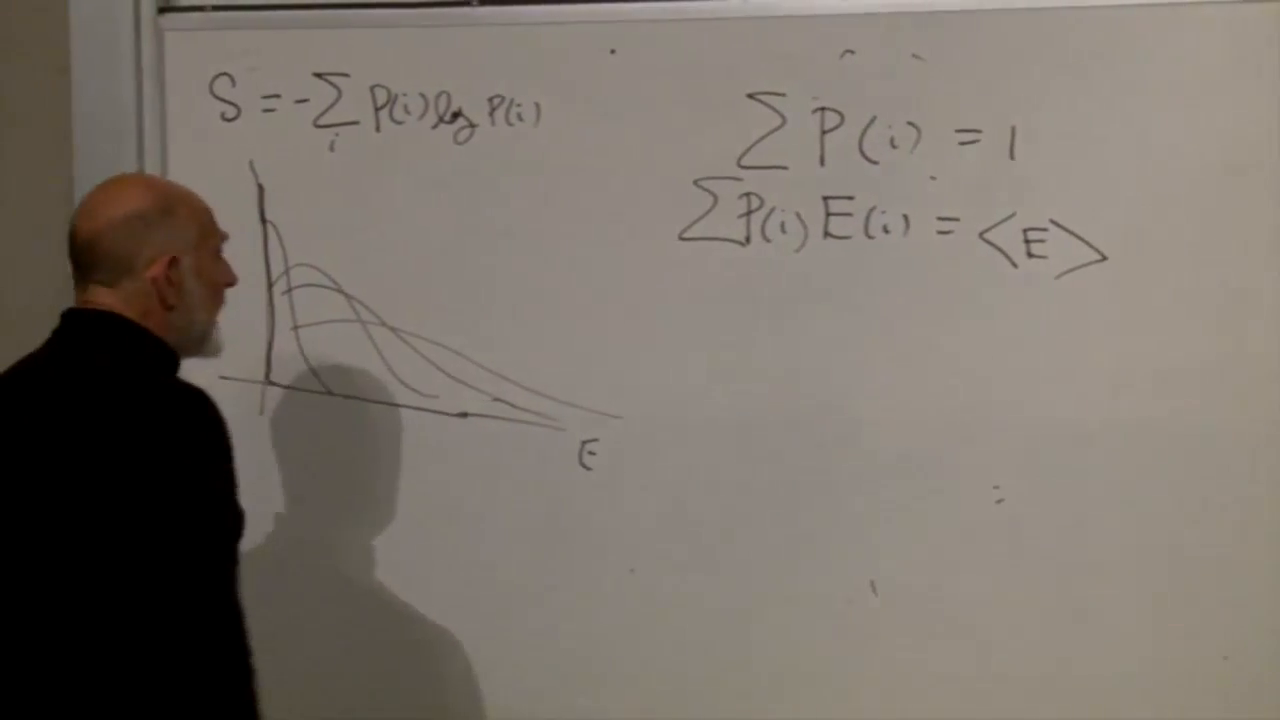
\includegraphics[width=0.88\textwidth]{lecture_03_figure_02.png}
\caption{Die erste Tafelansicht zeigt die Formeln für Entropie, Normierung und mittlere Energie sowie eine qualitative Familie von Gleichgewichtsverteilungen.}
\lectureframe{00:06:44}
\end{figure}

\section{Gleichgewicht als Familie von Verteilungen}

Aus der vorherigen Vorlesung ist eine von einem Parameter abhängige Familie von Gleichgewichtsverteilungen hervorgegangen. Man kann diese Familie durch die Temperatur parametrisieren, doch vorerst ist es nützlicher, sie durch die mittlere Energie \(\overline E\) zu kennzeichnen. Bei der kleinstmöglichen Energie ist die Verteilung auf einen Grundzustand konzentriert:
\[
 P_i=\delta_{i0}.
\]
Dann besteht keine Ungewissheit über den Zustand, und es gilt \(S=0\). Wenn sich die Gleichgewichtsverteilung über mehr Energieniveaus ausbreitet, steigen sowohl ihre mittlere Energie als auch ihre Entropie.

Diese Aussage gilt für die thermische Familie, nicht für jede denkbare Verteilungsfamilie. Eine beliebige Familie könnte sich zu höheren Energien verschieben und zugleich schmaler werden. Die herzuleitenden Gleichgewichtsverteilungen verhalten sich im gewöhnlichen Bereich positiver Temperaturen nicht so. Entlang dieser Familie gilt
\begin{equation}
 \frac{dS}{d\overline E}>0.
 \label{eq:sm3-positive-temperature-branch}
\end{equation}
Systeme mit beschränktem Spektrum können auch Zweige besitzen, auf denen diese Ableitung negativ ist. Diese Bereiche negativer Temperatur sind real, werden im vorliegenden Argument aber zunächst ausgeklammert.

Thermisches Gleichgewicht bedeutet mehr als mikroskopische Ruhe. Moleküle bewegen sich weiter, stoßen zusammen und tauschen Energie aus. Stationär geworden ist die makroskopische Beschreibung: Die Verteilung zeigt keine gerichtete Nettoverschiebung mehr, und getrennte Teile des Systems weisen keinen Nettoenergiefluss mehr auf.

\section{Die thermodynamischen Gesetze in statistischer Sprache}

Der erste Hauptsatz ist die Energieerhaltung. Der zweite Hauptsatz besagt, dass die thermodynamische Entropie eines isolierten makroskopischen Systems nicht abnimmt:
\begin{equation}
 \Delta S_{\mathrm{tot}}\geq0.
 \label{eq:sm3-second-law}
\end{equation}
Gleichheit beschreibt Gleichgewicht oder eine ideal reversible Änderung; bei einer spontanen Relaxation nimmt die Entropie gewöhnlich strikt zu.

In der probabilistischen Beschreibung verteilt sich das Gewicht bei der Relaxation tendenziell auf die makroskopischen Alternativen, die wir weiterhin unterscheiden. Hier ist die in der Vorlesung hervorgehobene Einschränkung wichtig: Wir führen eine \emph{Grobkörnung} durch. Die exakte Hamiltonsche Entwicklung erhält die feinkörnige Phasenraumentropie. Die makroskopische Entropie wächst, weil wir mikroskopische Korrelationen und Einzelheiten nicht mehr verfolgen. Dieser Informationsverlust verbreitert die reduzierte Beschreibung. Eine spontane Verengung würde hingegen bedeuten, dass wir ohne Messung mikroskopische Information erlangt hätten.

Das nullte Gesetz besagt, dass Systeme thermisches Gleichgewicht erreichen können und dass die Gleichgewichtsrelation transitiv ist. Befindet sich \(A\) mit \(B\) im Gleichgewicht und \(B\) mit \(C\), so befindet sich \(A\) mit \(C\) im Gleichgewicht. Die Temperatur liefert die Größe, die diese Transitivität unmittelbar sichtbar macht:
\[
 T_A=T_B,\qquad T_B=T_C
 \quad\Longrightarrow\quad
 T_A=T_C.
\]
Außerhalb des Gleichgewichts fließt Energie vom Teilsystem mit der höheren Temperatur zum Teilsystem mit der niedrigeren Temperatur. Bei gleichen Temperaturen kommt der Nettofluss zum Erliegen. Nun leiten wir diese operationale Aussage aus der Entropiedefinition der Temperatur her.

\section{Warum Energie von warm nach kalt fließt}

Betrachten wir zwei schwach gekoppelte Teilsysteme \(A\) und \(B\). Jedes befindet sich intern im Gleichgewicht, aber ihre Temperaturen unterscheiden sich. Die Bezeichnungen seien so gewählt, dass
\begin{equation}
 T_B>T_A>0.
 \label{eq:sm3-temperature-order}
\end{equation}
Bei einem kleinen Energieaustausch folgt aus der Energieerhaltung für das Gesamtsystem
\begin{equation}
 dE_A+dE_B=0.
 \label{eq:sm3-energy-conservation}
\end{equation}
Der zweite Hauptsatz verlangt
\begin{equation}
 dS_A+dS_B\geq0.
 \label{eq:sm3-entropy-change}
\end{equation}
Für jedes Teilsystem, das intern im Gleichgewicht ist, ist die Temperatur definiert durch
\begin{equation}
 dE_X=T_X\,dS_X,
 \qquad X=A,B.
 \label{eq:sm3-temperature-differential}
\end{equation}
Einsetzen in \eqref{eq:sm3-energy-conservation} ergibt
\begin{equation}
 T_A\,dS_A+T_B\,dS_B=0,
\end{equation}
und damit
\begin{equation}
 dS_B=-\frac{T_A}{T_B}\,dS_A.
 \label{eq:sm3-dsb}
\end{equation}
Setzen wir dieses Ergebnis in \eqref{eq:sm3-entropy-change} ein, so erhalten wir
\begin{align}
 dS_{\mathrm{tot}}
 &=dS_A-\frac{T_A}{T_B}dS_A\\
 &=\frac{T_B-T_A}{T_B}\,dS_A\geq0.
 \label{eq:sm3-flow-entropy}
\end{align}
Da \(T_B-T_A>0\) und \(T_B>0\) gilt, muss für einen spontanen Austausch
\[
 dS_A>0.
\]
Aus Gleichung \eqref{eq:sm3-temperature-differential} folgt dann
\begin{equation}
 dE_A=T_A\,dS_A>0,
 \qquad
 dE_B=-dE_A<0.
 \label{eq:sm3-hot-to-cold}
\end{equation}
Energie ist von \(B\), dem heißeren Teilsystem, zu \(A\), dem kälteren Teilsystem, geflossen. Wärme ist hier einfach Energie im Transit. Der Fluss hält an, bis \(T_A=T_B\) gilt; dann begünstigt die Entropieänderung erster Ordnung keine der beiden Richtungen mehr.

Dasselbe Ergebnis lässt sich in einer Zeile darstellen:
\begin{equation}
 dS_{\mathrm{tot}}
 =dE_A\left(\frac{1}{T_A}-\frac{1}{T_B}\right)\geq0.
 \label{eq:sm3-compact-flow}
\end{equation}
Das Vorzeichen der Differenz der inversen Temperaturen legt das Vorzeichen von \(dE_A\) fest. Diese kompakte Form wird sich später natürlich in das kanonische Ensemble einfügen.

\begin{classroomqa}
\audiencequestion{Setzt dieses Argument voraus, dass \(A\) und \(B\) jeweils bereits im inneren Gleichgewicht sind?}
\lecturerresponse{Ja. Die Zuweisung einer einzelnen Temperatur \(T_A\) beziehungsweise \(T_B\) setzt das voraus. Ist ein Teilsystem intern nicht im Gleichgewicht, teilt man es in kleinere Bereiche auf und wendet das Argument dort lokal an, wo sich eine Temperatur definieren lässt. Die globale Relaxation setzt sich dann aus Energieaustausch zwischen diesen Bereichen zusammen.
\lecturetimestamp{00:24:38--00:25:22}}
\end{classroomqa}

\section{Was gilt als Zustand?}

Bevor wir nach den Gleichgewichtswahrscheinlichkeiten fragen, müssen wir wissen, was die Bezeichnung \(i\) bedeutet. Ein mikroskopischer Zustand ist die vollständigste Beschreibung des Systems, die nach den zugrunde liegenden physikalischen Gesetzen möglich ist. In der klassischen Mechanik stellt man sich die Orte und Impulse aller Teilchen vor. In der Quantenmechanik ist ein Zustand stattdessen ein vollständiger Quantenzustand; die Unschärferelation verhindert eine gleichzeitige scharfe Festlegung sämtlicher klassischer Orte und Impulse.

Für ein Quantensystem in einer endlichen Box kann die relevante Zustandszählung diskret sein. Die klassische statistische Mechanik ergibt sich in einem geeigneten Grenzfall, in dem Summen über dicht liegende Quantenzustände in Phasenraumintegrale übergehen. Dieser Grenzübergang führt auch die Phasenraumzelle ein, die benötigt wird, um die kontinuierliche Entropie dimensionslos zu machen; sie ergibt sich nicht einfach dadurch, dass man ein Summenzeichen durch ein Integralzeichen ersetzt.

\begin{classroomqa}
\audiencequestion{Sollte man sich bei einem Gas einen Zustand als Ort und Impuls jedes einzelnen Moleküls vorstellen?}
\lecturerresponse{Das ist das richtige klassische Bild. Allgemeiner bezeichnet ein Zustand alles, was nach den physikalischen Gesetzen prinzipiell über das System bekannt sein kann. Die Quantenmechanik verändert die Form dieser maximalen Beschreibung und führt zu einer diskreten Zählung bei endlichem Volumen. Das klassische Integral aus der Quantensumme zurückzugewinnen, ist ein echter Grenzübergang und keine Substitution in einer Zeile.
\lecturetimestamp{00:25:31--00:27:38}}
\end{classroomqa}

\section{Ein Wärmebad aus Replikaten}

Die schwierige Frage lässt sich nun nicht mehr umgehen: Was bestimmt \(P_i\), nachdem sich das Gleichgewicht eingestellt hat?

Bringen wir das Teilsystem mit einem sehr großen Wärmebad in Kontakt. Energie kann hin und her fließen, doch das Bad hat so viele Freiheitsgrade, dass die Übertragung einer kleinen Energiemenge seine Temperatur kaum verändert. Ein besonders praktisches Bad besteht aus vielen schwach gekoppelten Replikaten des Teilsystems selbst. Ein Replikat ist das untersuchte System; die übrigen bilden seine Umgebung.

Diese Konstruktion bildet oft ein reales makroskopisches System nach. Man teile einen großen, annähernd homogenen Körper in viele ähnliche Zellen. Jede Zelle ist ein Teilsystem, und die übrigen Zellen bilden ihr Bad. Die Gesamtzahl der Replikate sei \(N\). Die Vorlesungsdemonstration verwendet neun Replikate und drei farblich gekennzeichnete Zustände; die Zählung hängt jedoch nicht von diesen konkreten Zahlen ab.

Sei \(n_i\) die Anzahl der Replikate im Zustand \(i\). Diese Größen heißen \emph{Belegungszahlen}. Es kann unendlich viele mögliche Energieniveaus geben, aber bei endlicher Gesamtenergie sind die Belegungszahlen der sehr hohen Niveaus meist vernachlässigbar oder gleich null.

Die erste Nebenbedingung betrifft schlicht die Zahl der Replikate:
\begin{equation}
 \sum_i n_i=N.
 \label{eq:sm3-number-constraint}
\end{equation}
Die zweite betrifft die Gesamtenergie:
\begin{equation}
 \sum_i n_iE_i=N\overline E.
 \label{eq:sm3-total-energy-constraint}
\end{equation}
Die rechte Seite ist eine extensive Größe. Verdoppelt man die Zahl der Replikate bei gleichbleibendem statistischem Zustand, so verdoppelt sich die Gesamtenergie, während die mittlere Energie pro Replikat \(\overline E\) bleibt.

\begin{classroomqa}
\audiencequestion{Muss die Replikatkonstruktion auch eine Energiebedingung erfüllen?}
\lecturerresponse{Ja. Die Belegungszahlen müssen sich zu \(N\) summieren, und ihre mit der Energie gewichtete Summe muss gleich der festgelegten Gesamtenergie \(N\overline E\) sein. Genau diese beiden Nebenbedingungen schränken später das Entropiemaximum ein.
\lecturetimestamp{00:37:12--00:39:54}}
\end{classroomqa}

Die Wahrscheinlichkeit, dass ein zufällig ausgewähltes Replikat den Zustand \(i\) einnimmt, ist seine relative Häufigkeit:
\begin{equation}
 P_i=\frac{n_i}{N},
 \qquad
 n_i=NP_i.
 \label{eq:sm3-frequency-probability}
\end{equation}

\begin{figure}[t]
\centering
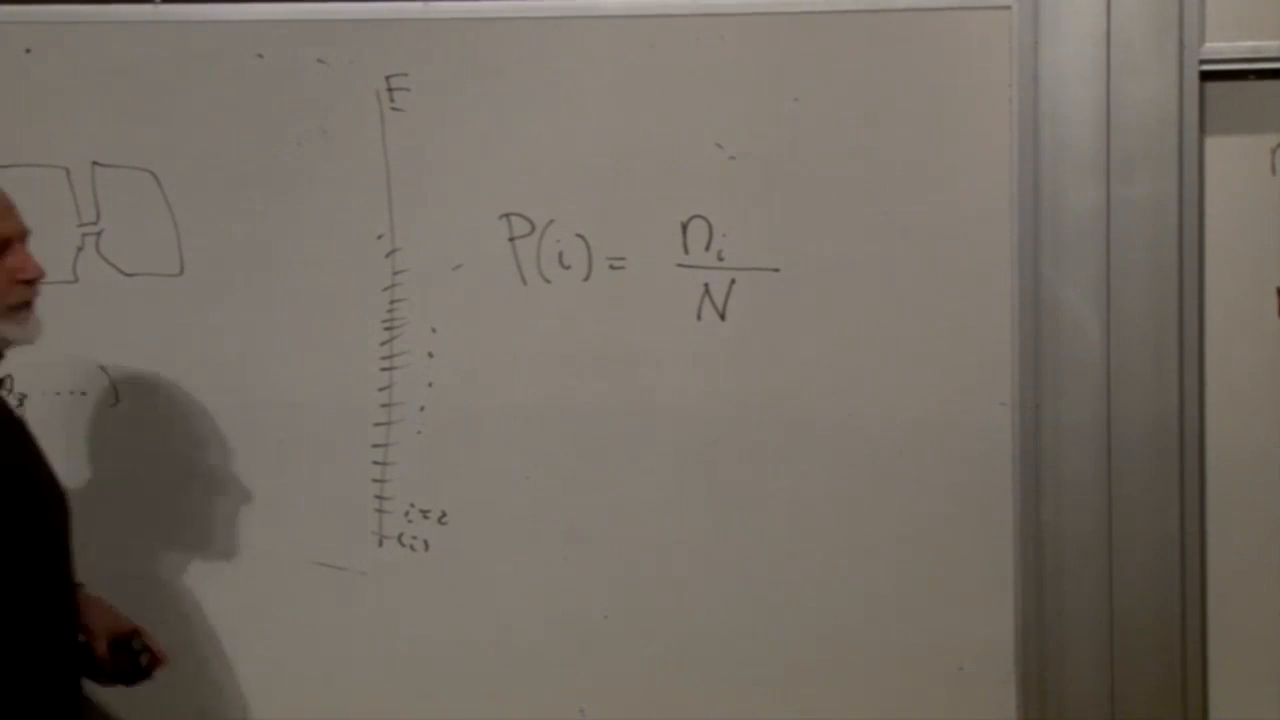
\includegraphics[width=0.82\textwidth]{lecture_03_figure_03.png}
\caption{Das Energieniveaubild und die Identifikation der Wahrscheinlichkeit mit dem Belegungsanteil \(P_i=n_i/N\)}
\lectureframe{00:41:40}
\end{figure}

\begin{classroomqa}
\audiencequestion{Soll die Schreibweise \(N(i)\) an der Tafel etwas anderes bezeichnen als \(n_i\)?}
\lecturerresponse{Nein. Beide bezeichnen die Belegungszahl des Zustands \(i\). Wir verwenden durchgängig \(n_i\) und reservieren das große \(N\) für die Gesamtzahl der Replikate.
\lecturetimestamp{00:41:28--00:41:33}}
\end{classroomqa}

Teilt man \eqref{eq:sm3-number-constraint} und \eqref{eq:sm3-total-energy-constraint} durch \(N\), so erhält man wieder die Wahrscheinlichkeitsbedingungen:
\begin{equation}
 \sum_iP_i=1,
 \qquad
 \sum_iP_iE_i=\overline E.
 \label{eq:sm3-probability-constraints}
\end{equation}
Die Häufigkeitsinterpretation im Ensemble liefert somit wieder die Gleichungen, mit denen wir begonnen haben.

\section{Multiplizität eines Belegungsmusters}

Wir legen einen Satz von Belegungszahlen \(\{n_i\}\) fest. Wie viele Zuordnungen der \(N\) unterscheidbaren Replikate zu den Zuständen ergeben genau diesen Satz? Die Antwort lautet: der Multinomialkoeffizient
\begin{equation}
 C(\{n_i\})=\frac{N!}{\prod_i n_i!}.
 \label{eq:sm3-multiplicity}
\end{equation}
Um den Nenner zu verstehen, ordnen wir zunächst alle \(N\) markierten Replikate auf \(N!\) verschiedene Arten an. Eine Permutation der \(n_i\) Replikate, die denselben Zustand einnehmen, ergibt keine neue Belegungszuordnung. Daher teilen wir für jeden Zustand durch \(n_i!\).

\begin{figure}[t]
\centering
\includegraphics[width=0.88\textwidth]{lecture_03_figure_04.png}
\caption{Die an der Tafel notierte Multinomialmultiplizität \(C=N!/\prod_i n_i!\)}
\lectureframe{00:46:55}
\end{figure}

Unbesetzte Niveaus bereiten kein Problem, denn \(0!=1\). Besetzen alle Replikate einen Zustand, so gilt erwartungsgemäß
\[
 C=\frac{N!}{N!}=1,
\]
Besetzen drei Replikate drei verschiedene, festgelegte Zustände, so gilt
\[
 C=\frac{3!}{1!\,1!\,1!}=6.
\]
Besetzen zwei Replikate zwei festgelegte Zustände, liefert die Formel zwei Zuordnungen: Man vertauscht, welches markierte Replikat welchen Zustand einnimmt.

\begin{classroomqa}
\audiencequestion{Kann mehr als ein Satz von Belegungszahlen die beiden Nebenbedingungen erfüllen?}
\lecturerresponse{In der Regel gibt es viele solche Sätze. Gleichung \eqref{eq:sm3-multiplicity} zählt zunächst die Anordnungen für einen einzelnen festgelegten Satz \(\{n_i\}\), ohne bereits zu entscheiden, ob dieser die Nebenbedingungen erfüllt. Im nächsten Schritt vergleichen wir alle mit den Nebenbedingungen verträglichen Sätze und bestimmen, welcher davon die größte Multiplizität hat.
\lecturetimestamp{00:48:07--00:48:43}}
\end{classroomqa}

Die statistische Annahme lautet, dass die mit dem isolierten Aufbau verträglichen mikroskopischen Zuordnungen gleichberechtigt behandelt werden. Ein makroskopisches Belegungsmuster, das durch mehr Zuordnungen realisiert wird, ist daher wahrscheinlicher. Für großes \(N\) wird die Verteilung der Anteile \(n_i/N\) stark um einen Wert konzentriert. Die Gleichgewichtsanteile sind die Werte, die \(C\) maximieren, unter den Nebenbedingungen \eqref{eq:sm3-number-constraint} und \eqref{eq:sm3-total-energy-constraint}.

\section{Die Stirling-Näherung}

Fakultäten werden schon lange bevor \(N\) makroskopisch groß ist enorm, daher betrachten wir ihre Logarithmen. Wir beginnen mit
\begin{equation}
 \log N!=\sum_{x=1}^{N}\log x.
 \label{eq:sm3-log-factorial-sum}
\end{equation}
Für großes \(N\) wird die Summe durch den Flächeninhalt unter \(\log x\) angenähert:
\begin{align}
 \log N!
 &\simeq\int_1^N\log x\,dx\\
 &=\left[x\log x-x\right]_1^N\\
 &=N\log N-N+1.
 \label{eq:sm3-stirling-integral}
\end{align}
Die Stammfunktion ergibt sich unmittelbar aus
\[
 \frac{d}{dx}(x\log x-x)=\log x.
\]
In führender extensiver Ordnung kann die additive Konstante weggelassen werden:
\begin{equation}
 \log N!\simeq N\log N-N.
 \label{eq:sm3-stirling-log}
\end{equation}
Durch Exponenzieren erhalten wir die in der Vorlesung verwendete vereinfachte Form,
\begin{equation}
 N!\simeq N^N e^{-N}.
 \label{eq:sm3-stirling-simple}
\end{equation}

\begin{figure}[t]
\centering
\includegraphics[width=0.88\textwidth]{lecture_03_figure_05.png}
\caption{Die führende Stirling-Näherung und ihre Herleitung, bei der die Summe von \(\log x\) durch ein Integral ersetzt wird.}
\lectureframe{01:03:45}
\end{figure}

\begin{classroomqa}
\audiencequestion{Bleibt bei der Auswertung von \(x\log x-x\) an der unteren Grenze ein zusätzliches \(+1\) übrig?}
\lecturerresponse{Ja. Gleichung \eqref{eq:sm3-stirling-integral} enthält diese Konstante. Sie ist gegenüber den zu \(N\) proportionalen Termen vernachlässigbar, wenn \(N\to\infty\), weshalb sie in der führenden Näherung weggelassen wird. Die Summe selbst muss bei \(x=1\) beginnen; \(\log0\) ist nicht definiert.
\lecturetimestamp{01:04:12--01:04:35}}
\end{classroomqa}

\begin{classroomqa}
\audiencequestion{Fehlt auch ein Faktor proportional zu \(\sqrt{N}\)?}
\lecturerresponse{Ja. Die genauere asymptotische Formel lautet
\[
 N!\sim\sqrt{2\pi N}\left(\frac{N}{e}\right)^N.
\]
Ihr Logarithmus liefert lediglich den Zusatzterm \(\tfrac12\log(2\pi N)\), der gegenüber \(N\log N-N\) subextensiv ist. Für genaue Wahrscheinlichkeiten bei endlichem \(N\) ist er relevant, nicht aber für die führende Entropieberechnung eines makroskopischen Systems.
\lecturetimestamp{01:04:35--01:05:40}}
\end{classroomqa}

Auch im Nenner von \eqref{eq:sm3-multiplicity} muss die Stirling-Näherung mit Bedacht angewendet werden. Im thermodynamischen Grenzfall gilt für die Zustände mit nichtverschwindenden Grenzwahrscheinlichkeiten \(n_i=NP_i\), sodass ihre Belegungszahlen mit \(N\) anwachsen. Zustände mit sehr kleiner oder verschwindender Belegung lassen sich mithilfe einer Abschneidung bei endlicher Energie behandeln, die man anschließend im Grenzfall wieder aufhebt. Die führende extensive Entropie bleibt von den weggelassenen Termen höherer Ordnung unberührt.

\section{Der Logarithmus der Multiplizität ist die Entropie}

Wenden wir \eqref{eq:sm3-stirling-simple} auf den Zähler und alle makroskopisch besetzten Faktoren im Nenner an:
\begin{equation}
 C\simeq
 \frac{N^Ne^{-N}}
 {\prod_i n_i^{\,n_i}e^{-n_i}}.
 \label{eq:sm3-c-stirling}
\end{equation}
Da \(\sum_i n_i=N\), kürzen sich die führenden Exponentialfaktoren heraus:
\begin{equation}
 C\simeq\frac{N^N}{\prod_i n_i^{\,n_i}}.
 \label{eq:sm3-c-leading}
\end{equation}
Der Logarithmus lässt sich leichter maximieren als ein Produkt; außerdem ist er monoton. Daher treten beide Maxima beim selben Belegungsmuster auf:
\begin{equation}
 \log C=N\log N-\sum_i n_i\log n_i.
 \label{eq:sm3-logc-occupations}
\end{equation}
Setzen wir nun \(n_i=NP_i\) ein:
\begin{align}
 \log C
 &=N\log N-\sum_iNP_i\log(NP_i)\\
 &=N\log N-N\sum_iP_i\log N
   -N\sum_iP_i\log P_i\\
 &=-N\sum_iP_i\log P_i,
 \label{eq:sm3-logc-entropy-derivation}
\end{align}
wobei sich die beiden Terme \(N\log N\) aufgrund der Normierung aufheben. Somit gilt in führender Ordnung für \(N\)
\begin{equation}
 \boxed{\log C=NS}.
 \label{eq:sm3-logc-ns}
\end{equation}

\begin{figure}[t]
\centering
\includegraphics[width=0.88\textwidth]{lecture_03_figure_06.png}
\caption{Die Tafelausführung, die \(\log C=N\log N-\sum_i n_i\log n_i\) mit \(-N\sum_iP_i\log P_i=NS\) verknüpft.}
\lectureframe{01:16:10}
\end{figure}

Diese Beziehung bildet den begrifflichen Kern des Kapitels. Die Entropie ist keine zusätzliche Größe, die dem Zählproblem äußerlich auferlegt wird. Sie ist die logarithmisch gemessene Multiplizität pro Replikat. Die Zahl der mikroskopischen Anordnungen zu maximieren, ist daher in führender Ordnung gleichbedeutend damit, die Entropie eines einzelnen Replikats zu maximieren.

\begin{classroomqa}
\audiencequestion{Wäre die Multiplizität nicht am größten, wenn alle Belegungszahlen gleich wären?}
\lecturerresponse{Bei einer endlichen Zahl von Zuständen ist die Verteilung gleichförmig, wenn kein Zustand ausgezeichnet ist und nur \(\sum_i n_i=N\) vorgegeben wird. Die Bedingung fester Energie ändert das Ergebnis, weil die Werte \(E_i\) verschieden sind. Gleiche Belegungszahlen ergeben im Allgemeinen nicht die vorgegebene mittlere Energie.
\lecturetimestamp{01:17:07--01:18:20}}
\end{classroomqa}

\begin{classroomqa}
\audiencequestion{Das große \(N\) ist zwar groß, aber warum darf die Stirling-Näherung auf jedes \(n_i\) im Nenner angewendet werden?}
\lecturerresponse{Für jeden Zustand mit einer von null verschiedenen Grenzwahrscheinlichkeit wächst \(n_i=NP_i\) proportional zu \(N\). Man kann zunächst einen endlichen Energiebereich beibehalten, darin den Grenzfall großer \(N\) bilden und anschließend den Bereich erweitern. Selten besetzte Zustände im Ausläufer erfordern eigene endliche Korrekturen, ändern aber nichts an der führenden extensiven Entropie.
\lecturetimestamp{01:18:23--01:19:28}}
\end{classroomqa}

\begin{classroomqa}
\audiencequestion{Ist diese Näherung für große \(N\) das, was zuvor mit Grobkörnung gemeint war?}
\lecturerresponse{Nein. Der thermodynamische Grenzfall behandelt große Belegungszahlen und asymptotische Zählung. Grobkörnung bedeutet den Verlust oder das bewusste Verwerfen mikroskopischer Auflösung. Es handelt sich um verschiedene Vorgänge, auch wenn beide in der makroskopischen statistischen Mechanik häufig verwendet werden.
\lecturetimestamp{01:19:29--01:19:46}}
\end{classroomqa}

\begin{classroomqa}
\audiencequestion{Da \(\log C=N\log N-\sum_i n_i\log n_i\), müsste dann nicht der zweite Term minimiert statt maximiert werden?}
\lecturerresponse{Ja; bei festem \(N\) ist die Maximierung von \(\log C\) gleichbedeutend mit der Minimierung von \(\sum_i n_i\log n_i\). Nach dem Einsetzen von \(n_i=NP_i\) heben sich die konstanten Terme \(N\log N\) auf, und übrig bleibt \(-N\sum_iP_i\log P_i=NS\). Daher lässt sich derselbe Vorgang natürlicher als Maximierung der positiven Entropie \(S\) beschreiben.
\lecturetimestamp{01:19:48--01:20:55}}
\end{classroomqa}

\begin{classroomqa}
\audiencequestion{Warum schließen wir das Argument nicht sofort aufgrund der Symmetrie ab und setzen alle \(n_i\) gleich?}
\lecturerresponse{Diese Abkürzung ignoriert die Energiebezeichnungen. Die Normierungsbedingung behandelt die Zustände symmetrisch, aber \(\sum_iP_iE_i=\overline E\) tut dies nicht: Zustände mit verschiedenen Energien tragen unterschiedlich bei. Genau durch die Energiebedingung kommt die nichtgleichförmige Gleichgewichtsverteilung ins Spiel.
\lecturetimestamp{01:21:15--01:21:41}}
\end{classroomqa}

\section{Das Problem der maximalen Entropie}

Nun können wir die Regel der statistischen Mechanik eindeutig formulieren. Wir variieren die Wahrscheinlichkeiten \(P_i\) und maximieren
\begin{equation}
 S[P]=-\sum_iP_i\log P_i
 \label{eq:sm3-maximize-entropy}
\end{equation}
unter den Nebenbedingungen
\begin{equation}
 \sum_iP_i=1,
 \qquad
 \sum_iP_iE_i=\overline E.
 \label{eq:sm3-maxent-constraints}
\end{equation}
Die maximierenden Wahrscheinlichkeiten geben die stark bevorzugten Belegungsanteile eines großen Replikatensembles an. Die Belegungszahlen fluktuieren, doch ihre relativen Abweichungen werden mit wachsendem \(N\) kleiner, sodass die Verhältnisse \(n_i/N\) zu wohldefinierten thermodynamischen Wahrscheinlichkeiten werden.

\begin{classroomqa}
\audiencequestion{Sind die Zustandsenergien \(E_i\) fest vorgegeben, während die Nebenbedingung eine separat vorgegebene Gesamtenergie verwendet?}
\lecturerresponse{Ja. Das Spektrum \(\{E_i\}\) gehört zum Teilsystem. Die Gesamtenergie der vollständigen Replikatsammlung ist fest, aber Energie wird fortwährend zwischen den Replikaten übertragen. Wenn man diese Gesamtenergie durch \(N\) teilt, erhält man die mittlere Energie \(\overline E\) eines Replikats, nicht seine Energie in jeder einzelnen mikroskopischen Realisierung.
\lecturetimestamp{01:26:12--01:27:07}}
\end{classroomqa}

Das Problem ist leicht zu formulieren, aber noch nicht gelöst. Es handelt sich um ein Extremierungsproblem mit zwei Nebenbedingungen; dafür benötigen wir noch ein mathematisches Hilfsmittel.

\section{Lagrange-Multiplikatoren}

Für eine unbeschränkte Funktion \(F(x_1,x_2,\ldots)\) erfüllt ein stationärer Punkt die Bedingung
\begin{equation}
 \frac{\partial F}{\partial x_i}=0
 \qquad\text{for every }i.
 \label{eq:sm3-unconstrained-stationary}
\end{equation}
Nun verlangen wir zusätzlich
\begin{equation}
 G(x_1,x_2,\ldots)=0.
 \label{eq:sm3-one-constraint}
\end{equation}

\begin{classroomqa}
\audiencequestion{Was bedeutet \(x\), wenn die Darstellung die Koordinaten \(x\) und \(y\) verwendet?}
\lecturerresponse{Hier ist \(x\) eine Kurzschreibweise für den gesamten Koordinatenvektor \((x_1,x_2,\ldots)\). In der zweidimensionalen Darstellung sind seine Komponenten einfach \(x\) und \(y\). Später werden die Komponenten die Wahrscheinlichkeiten \(P_1,P_2,\ldots\) sein.
\lecturetimestamp{01:30:12--01:30:20}}
\end{classroomqa}

Geometrisch bilden die Niveaukurven \(F=\text{constant}\) eine Höhenlinienkarte, während \(G=0\) die Kurve ist, auf der sich das System bewegen darf. Ein Extremum unter einer Nebenbedingung liegt dort, wo eine Niveaukurve von \(F\) die Nebenbedingungskurve berührt. An diesem Punkt sind die Gradienten parallel:
\begin{equation}
 \nabla F=-\lambda\nabla G
 \label{eq:sm3-parallel-gradients}
\end{equation}
für eine Zahl \(\lambda\).

\begin{figure}[t]
\centering
\includegraphics[width=0.88\textwidth]{lecture_03_figure_07.png}
\caption{Die Konturgeometrie an der Tafel und die erweiterte Funktion \(F'=F+\lambda G\). Ein Extremum unter einer Nebenbedingung liegt am Berührungspunkt.}
\lectureframe{01:37:10}
\end{figure}

Gleichung \eqref{eq:sm3-parallel-gradients} erhält man, indem man die erweiterte Funktion
\begin{equation}
 F'=F+\lambda G
 \label{eq:sm3-augmented-function}
\end{equation}
definiert und gewöhnliche Stationarität fordert:
\begin{equation}
 \frac{\partial F'}{\partial x_i}=0.
 \label{eq:sm3-augmented-stationarity}
\end{equation}
Der Multiplikator \(\lambda\) ist zunächst unbekannt. Dadurch ist das Gleichungssystem nicht unterbestimmt, denn die ursprüngliche Nebenbedingung \(G=0\) liefert eine zusätzliche Gleichung.

\begin{classroomqa}
\classquestion{Warum macht ein Term proportional zu \(G\) den Punkt unter der Nebenbedingung stationär?}
\lecturerresponse{Am Extremum unter der Nebenbedingung verursacht eine Bewegung tangential zu \(G=0\) bereits keine Änderung erster Ordnung von \(F\). Die einzige verbleibende Steigung steht normal auf der Nebenbedingung. Da \(\nabla G\) in dieselbe Normalenrichtung zeigt, lässt sie sich durch eine geeignete Wahl von \(\lambda\) aufheben:
\(\nabla F+\lambda\nabla G=0\).
\lecturetimestamp{01:35:06--01:35:32}}
\end{classroomqa}

\section{Ein Beispiel mit zwei Variablen}

Minimiere
\begin{equation}
 F(x,y)=\frac{x^2+y^2}{2}
 \label{eq:sm3-example-f}
\end{equation}
unter der Nebenbedingung
\begin{equation}
 x+y=1.
 \label{eq:sm3-example-constraint}
\end{equation}
Schreiben wir die Nebenbedingung als \(G=x+y-1=0\) und bilden
\begin{equation}
 F'=\frac{x^2+y^2}{2}+\lambda(x+y-1).
 \label{eq:sm3-example-augmented}
\end{equation}
Die Stationaritätsgleichungen lauten
\begin{align}
 \frac{\partial F'}{\partial x}&=x+\lambda=0,\\
 \frac{\partial F'}{\partial y}&=y+\lambda=0.
 \label{eq:sm3-example-derivatives}
\end{align}
Also gilt \(x=y=-\lambda\). Die verbleibende Gleichung ist die Nebenbedingung,
\[
 x+y=-2\lambda=1,
\]
und somit
\begin{equation}
 \lambda=-\frac12,
 \qquad
 x=y=\frac12.
 \label{eq:sm3-example-solution}
\end{equation}
Der Punkt \((1/2,1/2)\) ist der Punkt, an dem der kleinste Kreis mit Mittelpunkt im Ursprung die Gerade \(x+y=1\) berührt.

\begin{figure}[t]
\centering
\includegraphics[width=0.88\textwidth]{lecture_03_figure_08.png}
\caption{Die vollständige Rechnung mit Lagrange-Multiplikatoren zur Minimierung von \((x^2+y^2)/2\) unter der Nebenbedingung \(x+y=1\)}
\lectureframe{01:44:10}
\end{figure}

Bei mehreren Nebenbedingungen führen wir für jede einen Multiplikator ein:
\begin{equation}
 F'=F+\lambda_1G_1+\lambda_2G_2+\cdots.
 \label{eq:sm3-many-multipliers}
\end{equation}
Dann lösen wir
\begin{equation}
 \begin{aligned}
 \frac{\partial F'}{\partial x_i}&=0
 &&\text{for every }i,\\
 G_a&=0
 &&\text{for every constraint }a.
 \end{aligned}
 \label{eq:sm3-many-equations}
\end{equation}
Die Vorlesung schlägt als Übungsaufgabe bewusst ein künstliches Beispiel vor: Eine quadratische Funktion der Variablen \(x,y,z\) soll extremiert werden, während zwei unabhängige lineare Nebenbedingungen auferlegt werden, etwa \(x+y=1\) und \(z+x=1\). Entscheidend ist nicht die konkrete Lösung, sondern die Regel: Zu jeder Nebenbedingung gehören ein Multiplikator und eine Gleichung.

\section{Das Problem für die nächste Vorlesung}

In der statistischen Mechanik sind die Koordinaten die Wahrscheinlichkeiten \(\{P_i\}\), die zu maximierende Funktion ist die Entropie, und die Nebenbedingungen sind Normierung und feste mittlere Energie. Wir definieren
\begin{align}
 S[P]&=-\sum_iP_i\log P_i,\\
 G_1[P]&=\sum_iP_i-1,\\
 G_2[P]&=\sum_iP_iE_i-\overline E.
 \label{eq:sm3-final-functions}
\end{align}
Die erweiterte Entropie lässt sich daher schreiben als
\begin{equation}
 \Phi[P]
 =S[P]+\alpha G_1[P]+\beta G_2[P].
 \label{eq:sm3-final-augmented}
\end{equation}
Zu lösen sind die Gleichungen
\begin{equation}
 \frac{\partial\Phi}{\partial P_i}=0
 \quad\text{for every }i,
 \qquad
 G_1=0,
 \qquad
 G_2=0.
 \label{eq:sm3-final-problem}
\end{equation}

\begin{figure}[H]
\centering
\includegraphics[width=0.88\textwidth]{lecture_03_figure_09.png}
\caption{Die abschließende Tafelansicht: die Entropie als Funktion der Wahrscheinlichkeiten zusammen mit der Normierung und der festen mittleren Energie.}
\lectureframe{01:53:05}
\end{figure}

Damit ist das Problem vollständig formuliert. Durch Lösen von \eqref{eq:sm3-final-problem} erhält man die Gleichgewichtsverteilung. Der zur Energie konjugierte Multiplikator wird zur inversen Temperatur \(\beta=1/T\), bis auf die in \eqref{eq:sm3-final-augmented} gewählte Vorzeichenkonvention. In der nächsten Vorlesung führen wir diese Differentiation aus und erhalten die Boltzmann-Gewichte.

\chapter{Boltzmann-Gewichte, Zustandssummen und das ideale Gas}

\lectureoverview{Wir leiten die Gleichgewichts-\\Wahrscheinlichkeitsverteilung her, indem wir die Entropie bei fester Normierung und festem mittlerem Energieinhalt maximieren. Aus der Zustandssumme ergeben sich dann durch Ableiten der mittlere Energieinhalt, die Entropie und die Temperatur. Das ideale Gas liefert das erste vollständige Beispiel; anschließend folgen eine Erweiterung um die Gravitation und ein Ausblick auf Energieschwankungen.}

\section{Das Entropieproblem mit Nebenbedingungen}

Betrachten wir zunächst eine große Ansammlung von \(\mathcal N\) identischen, sehr schwach miteinander wechselwirkenden Replikaten desselben Teilsystems. Besetzen \(n_i\) Replikate den \(i\)-ten Zustand, so gilt
\begin{equation}
 p_i=\frac{n_i}{\mathcal N},
 \qquad
 \sum_i p_i=1.
 \label{eq:sm4-occupation-probability}
\end{equation}
Die kombinatorische Zählung aus der vorangegangenen Vorlesung ergibt die Entropie pro Replikat:
\begin{equation}
 S[p]=-\sum_i p_i\log p_i.
 \label{eq:sm4-entropy}
\end{equation}
Es lohnt sich, dies als gewöhnliche Funktion aller Variablen \(p_1,p_2,\ldots\) aufzufassen. Ihre einfache additive Form macht die Rechnung möglich.

Die Replikatansammlung hat eine feste Gesamtenergie \(\mathcal N E\), wobei \(E\) die mittlere Energie pro Replikat ist. Die zweite Nebenbedingung lautet daher
\begin{equation}
 \sum_i p_iE_i=E.
 \label{eq:sm4-energy-constraint}
\end{equation}
Die Energieniveaus \(E_i\) gehören zum Teilsystem; die Zahl \(E\) auf der rechten Seite ist ihr mit den Wahrscheinlichkeiten gewichteter Mittelwert. Die Maximierung von \eqref{eq:sm4-entropy} unter den Nebenbedingungen \eqref{eq:sm4-occupation-probability} und \eqref{eq:sm4-energy-constraint} wählt die mit überwältigender Wahrscheinlichkeit auftretenden Besetzungsanteile aus.

Der Einfachheit halber minimieren wir \(-S=\sum_i p_i\log p_i\). Für jede Nebenbedingung führen wir einen Lagrange-Multiplikator ein:
\begin{equation}
 \begin{aligned}
 \Phi[p;\alpha,\beta]
 &=\sum_i p_i\log p_i\\
 &\quad+\alpha\left(\sum_i p_i-1\right)\\
 &\quad+\beta\left(\sum_i p_iE_i-E\right).
 \end{aligned}
 \label{eq:sm4-augmented-functional}
\end{equation}
Die Bezeichnungen \(\alpha\) und \(\beta\) beruhen noch auf keinen physikalischen Annahmen. In diesem Stadium sind sie lediglich die beiden Zahlen, die zur Durchsetzung der beiden Nebenbedingungen erforderlich sind.

\begin{classroomqa}
\audiencequestion{Ist die erweiterte Funktion auch eine Funktion von \(\alpha\) und \(\beta\)?}
\lecturerresponse{Ja. Durch Variation nach \(\alpha\) und \(\beta\) erhält man wieder die beiden Nebenbedingungen. Für die unmittelbare Rechnung halten wir diese Multiplikatoren jedoch fest und variieren die Wahrscheinlichkeiten \(p_i\). Ihre Werte werden anschließend durch die Normierung und den vorgegebenen mittleren Energieinhalt festgelegt.
\lecturetimestamp{00:09:32--00:09:49}}
\end{classroomqa}

\begin{figure}[t]\centering
\includegraphics[width=0.92\textwidth]{lecture_04_figure_02.png}\caption{}\lectureframe{00:10:56}\end{figure}

Bei der Ableitung nach einer Wahrscheinlichkeit tragen die Terme \(-\alpha\) und \(-\beta E\) nichts bei. Dies ist die verkürzte Form des Funktionals, die an der Tafel zu sehen ist. Sie bleiben Bestandteil von \eqref{eq:sm4-augmented-functional}; für diese konkrete Ableitung sind sie lediglich irrelevant geworden.

\section{Die Boltzmann-Verteilung}

Wir wählen eine beliebige Wahrscheinlichkeit aus. In der Vorlesung wird \(p_7\) gewählt, unter anderem, weil \(1\) zu speziell wirkt und \(7\) eine Glückszahl ist. Von dieser Wahl hängt nichts ab. Die einzige benötigte Ableitung lautet
\begin{equation}
 \frac{d}{dp_i}\bigl(p_i\log p_i\bigr)=\log p_i+1.
\end{equation}
Damit gilt
\begin{equation}
 \frac{\partial\Phi}{\partial p_i}
 =\log p_i+1+\alpha+\beta E_i=0.
 \label{eq:sm4-stationarity}
\end{equation}
Aufgelöst nach \(p_i\) ergibt sich
\begin{align}
 \log p_i&=-(1+\alpha)-\beta E_i,\\
 p_i&=e^{-(1+\alpha)}e^{-\beta E_i}.
\end{align}
Der erste Faktor hängt nicht von der Zustandsbezeichnung ab. Wir schreiben ihn als \(1/Z\):
\begin{equation}
 p_i=\frac{e^{-\beta E_i}}{Z}.
 \label{eq:sm4-boltzmann-weight}
\end{equation}

Dies ist der erste unmittelbare Ertrag. Eine routinemäßige Ableitung unter Nebenbedingungen hat ein Exponentialgesetz ergeben. Die relativen Wahrscheinlichkeiten erfüllen
\begin{equation}
 \frac{p_i}{p_j}=e^{-\beta(E_i-E_j)}.
 \label{eq:sm4-relative-weight}
\end{equation}
Der Multiplikator \(\beta\) bestimmt, wie rasch die Wahrscheinlichkeit mit der Energie abnimmt. Große positive Werte von \(\beta\) konzentrieren die Verteilung auf die niedrigsten Energieniveaus; bei kleinen positiven Werten von \(\beta\) verteilt sich ein merklicher Anteil der Wahrscheinlichkeit weiter über das Spektrum. Wir sehen bereits, dass eine Änderung von \(\beta\) die mittlere Energie verändert, auch wenn noch zu beweisen ist, dass dieser Parameter mit der inversen Temperatur übereinstimmt.

\section{Normierung und Zustandssumme}

Die Normierung bestimmt den zustandsunabhängigen Faktor:
\begin{equation}
 1=\sum_i p_i
 =\frac{1}{Z}\sum_i e^{-\beta E_i},
\end{equation}
also
\begin{equation}
 Z(\beta)=\sum_i e^{-\beta E_i}.
 \label{eq:sm4-partition-function}
\end{equation}
Dies ist die kanonische Zustandssumme. Zunächst trat sie als Normierungskonstante auf, doch das wird ihrer Bedeutung kaum gerecht. Ist \(Z(\beta)\) erst einmal bekannt, ergeben sich thermodynamische Größen aus ihren Ableitungen.

Die Energieniveaus in \eqref{eq:sm4-partition-function} sind Eingangsgrößen. Sie ergeben sich aus der Mechanik des Systems und den festgelegten äußeren Bedingungen: Volumen und Form des Behälters, magnetische oder elektrische Felder sowie weitere Kontrollparameter. Eine Änderung eines Kontrollparameters verändert das Spektrum und damit \(Z\). Für die vorliegende Rechnung halten wir diese Parameter und somit auch die Menge \(\{E_i\}\) fest.

\begin{classroomqa}
\audiencequestion{Was genau stellen die Achsen der Exponentialskizze dar? Ist die vertikale Koordinate ein bestimmtes \(p_i\)?}
\lecturerresponse{Die eingezeichnete Höhe ist die einem Niveau zugeordnete Wahrscheinlichkeit. Die horizontale Anordnung kann entweder als Zustandsbezeichnung \(i\) oder, physikalisch anschaulicher, als Energie \(E_i\) gelesen werden. Jeder Zustand hat eine feste Energie. Bei großem \(\beta\) nimmt die Wahrscheinlichkeit mit dieser Energie steil ab; in der Nähe von \(\beta=0\) sind die Gewichte über die zugänglichen Niveaus nahezu gleich.
\lecturetimestamp{00:19:39--00:20:09}}
\end{classroomqa}

\section{Der im Inneren der Zustandssumme verborgene mittlere Energieinhalt}

Die zweite Nebenbedingung bestimmt \(\beta\):
\begin{equation}
 E=\sum_i p_iE_i
 =\frac{1}{Z}\sum_i E_i e^{-\beta E_i}.
 \label{eq:sm4-mean-energy}
\end{equation}
Statt diese gewichtete Summe erneut auszuwerten, leiten wir \eqref{eq:sm4-partition-function} ab:
\begin{equation}
 \frac{dZ}{d\beta}
 =-\sum_i E_i e^{-\beta E_i}.
\end{equation}
Der Vergleich mit \eqref{eq:sm4-mean-energy} ergibt
\begin{equation}
 E(\beta)
 =-\frac{1}{Z}\frac{dZ}{d\beta}
 =-\frac{d\log Z}{d\beta}.
 \label{eq:sm4-energy-logz}
\end{equation}
Der Logarithmus ist natürlich, weil seine Ableitung den Faktor \(1/Z\) liefert.

\begin{figure}[t]
\centering
\includegraphics[width=0.82\textwidth]{lecture_04_figure_03.png}
\caption{Normierung, Nebenbedingung für die mittlere Energie und Ableitung der Zustandssumme stehen gemeinsam an der Tafel.}
\lectureframe{00:26:24}
\end{figure}

\begin{classroomqa}
\audiencequestion{Ist die untere Gleichung an der Tafel eine neue Gleichung für \(Z\), oder folgt sie aus der darüberstehenden Definition?}
\lecturerresponse{Sie ergibt sich durch Ableiten der Definition \(Z=\sum_i e^{-\beta E_i}\). Durch die Ableitung erhält man den Faktor \(-E_i\). Teilt man das Ergebnis durch \(Z\), erhält man wieder die gewichtete Summe, die den mittleren Energieinhalt definiert.
\lecturetimestamp{00:25:58--00:26:37}}
\end{classroomqa}

\begin{classroomqa}
\audiencequestion{Macht \(dZ/d\beta=-E Z\) die Funktion \(Z\) zu einer Eigenfunktion der Ableitung?}
\lecturerresponse{Nicht im üblichen Sinn. In einer Eigenwertgleichung würde eine Konstante mit \(Z\) multipliziert; hier gilt jedoch \(E=E(\beta)\). Die Gleichung gibt den mittleren Energieinhalt als Funktion von \(\beta\) an; es handelt sich nicht um ein Problem mit festem Eigenwert.
\lecturetimestamp{00:28:49--00:29:43}}
\end{classroomqa}

Die Einfachheit von \eqref{eq:sm4-energy-logz} täuscht. Das Spektrum kann kompliziert sein, und die Berechnung von \(Z\) kann schwierig sein. Sobald diese eine Funktion jedoch gefunden ist, ergibt sich der mittlere Energieinhalt durch eine einzige Ableitung. Dieses Muster begegnet uns in der gesamten statistischen Mechanik: Richtig aufeinanderfolgende elementare Rechenschritte liefern Ergebnisse, die sich direkt nur schwer erraten ließen.

\begin{classroomqa}
\audiencequestion{Ist \(E\) die Gesamtenergie aller Replikate oder die mittlere Energie pro Behälter?}
\lecturerresponse{Es ist die mittlere Energie eines einzelnen Behälters. Die Replikatansammlung hat die Gesamtenergie \(\mathcal N E\). Später, wenn das System selbst als ein ganzer Behälter mit \(N\) Gasteilchen gewählt wird, bezeichnet \(E\) die Energie dieser gesamten Gasprobe.
\lecturetimestamp{00:30:55--00:31:10}}
\end{classroomqa}

\begin{classroomqa}
\audiencequestion{Können wir den Logarithmus von \(\sum_i e^{-\beta E_i}\) gliedweise nehmen?}
\lecturerresponse{Nein. Ein Logarithmus macht aus einem Produkt eine Summe, aber aus einer Summe keine Summe von Logarithmen:
\[
 \log\!\left(\sum_i e^{-\beta E_i}\right)
 \ne \sum_i\log\!\left(e^{-\beta E_i}\right).
\]
Diese Unterscheidung wird später nützlich, wenn sich die Zustandssummen unabhängiger Teilsysteme multiplizieren.
\lecturetimestamp{00:31:10--00:31:58}}
\end{classroomqa}

\section{Was ist festgelegt, und was darf variieren?}

In denselben Formeln kommen mehrere Ebenen von Variablen vor; in der Vorlesung werden sie bewusst getrennt betrachtet.

\begin{itemize}
 \item Die Wahrscheinlichkeiten \(p_i\) sind die ursprünglich unbekannten Größen.
 \item Die Energieniveaus \(E_i\) sind festgelegt, sobald das System und seine Kontrollparameter vorgegeben sind.
 \item Der Multiplikator \(\alpha\) ist in der Normierung \(Z=e^{1+\alpha}\) aufgegangen.
 \item Bei vorgegebenem mittlerem Energieinhalt \(E\) legt die Nebenbedingung eine Zahl \(\beta\) fest. Betrachtet man jedoch eine Familie von Gleichgewichtszuständen, kann man wahlweise \(E=E(\beta)\) oder \(\beta=\beta(E)\) verwenden.
\end{itemize}

\begin{classroomqa}
\audiencequestion{Wenn die Multiplikatoren Zahlen sind, warum werden \(\beta\) und \(E\) jetzt als Variablen behandelt?}
\lecturerresponse{Für ein einzelnes Problem mit Nebenbedingungen sind es tatsächlich Zahlen. Wir können aber viele Gleichgewichtsprobleme mit demselben Spektrum und unterschiedlichen vorgegebenen mittleren Energieinhalten vergleichen. Innerhalb dieser Familie ändert sich \(\beta\) mit \(E\). Die Festlegung von \(E\) bestimmt \(\beta\); die Festlegung von \(\beta\) bestimmt \(E\). Dies sind zwei Betrachtungsweisen derselben Beziehung.
\lecturetimestamp{00:31:58--00:33:27}}
\end{classroomqa}

\begin{classroomqa}
\audiencequestion{Ist \(\alpha\) verschwunden?}
\lecturerresponse{Nur seine Bezeichnung ist verschwunden. Die Definition \(e^{-(1+\alpha)}=1/Z\) nimmt es in \(Z\) auf. Würden wir sowohl \(\alpha\) als auch \(Z\) beibehalten, zählten wir denselben Normierungsparameter doppelt.
\lecturetimestamp{00:33:29--00:33:49}}
\end{classroomqa}

Energie muss nicht die einzige Erhaltungsgröße sein. Sind der Gesamtimpuls, die Teilchenzahl, der Drehimpuls oder eine andere Größe festgelegt, erhält ihr Erwartungswert jeweils einen eigenen Multiplikator. Diese Erweiterung ändert das Ensemble, nicht aber die Methode.

\begin{classroomqa}
\audiencequestion{Setzt die Festlegung allein des mittleren Energieinhalts zu viel über das System voraus?}
\lecturerresponse{Sie setzt voraus, dass im vorliegenden Problem keine weitere Erhaltungsgröße berücksichtigt werden muss. Ist beispielsweise auch der Gesamtimpuls festgelegt, fügen wir eine weitere Nebenbedingung und einen weiteren Lagrange-Multiplikator hinzu. Volumen, Form und äußere Felder sind hier dagegen Kontrollparameter: Sie werden festgehalten und bestimmen die Energieniveaus selbst.
\lecturetimestamp{00:33:51--00:35:50}}
\end{classroomqa}

\begin{classroomqa}
\audiencequestion{Sollte \(\alpha\) als weiteres Argument der Energie auftreten, und hängt \(Z\) von den Energieniveaus \(E_i\) ab?}
\lecturerresponse{\(\alpha\) ist bereits in \(Z\) enthalten und daher kein unabhängiges Argument. Die Zustandssumme hängt selbstverständlich sowohl vom festen Spektrum als auch von \(\beta\) ab. Eine Änderung eines Kontrollparameters verändert die \(E_i\) und damit auch \(Z\); bei den Ableitungen nach \(\beta\) in der vorliegenden Rechnung wird das Spektrum festgehalten.
\lecturetimestamp{00:35:52--00:37:10}}
\end{classroomqa}

\begin{classroomqa}
\audiencequestion{Variieren wir die einzelnen Energieniveaus \(E_i\) oder den mittleren Energieinhalt \(E\)?}
\lecturerresponse{Die einzelnen Energieniveaus bleiben fest. Der mittlere Energieinhalt ändert sich, weil sich die Wahrscheinlichkeiten ändern. Die Familie wird also durch \(E\) oder, gleichwertig, durch \(\beta\) parametrisiert; dabei wird stets dieselbe Liste von Energieniveaus \(\{E_i\}\) verwendet.
\lecturetimestamp{00:37:12--00:39:04}}
\end{classroomqa}

In der Praxis lässt sich die Temperatur oft viel leichter messen als die Gesamtenergie eines Gases. Wir können ein Thermometer einsetzen; den relativistischen Massendifferenz zu messen und \(E=mc^2\) heranzuziehen wäre zwar korrekt, aber ausgesprochen unpraktisch. Um \(\beta\) operational zu definieren, müssen wir es nun mit der thermodynamischen Temperaturdefinition verknüpfen.

\section{Die Entropie kommt vor der Temperatur}

Logisch kommt zuerst die Entropie. Wir setzen die Boltzmann-Wahrscheinlichkeiten in \eqref{eq:sm4-entropy} ein:
\begin{equation}
 \log p_i=-\beta E_i-\log Z.
\end{equation}
Dann folgt
\begin{align}
 S
 &=-\sum_i p_i\log p_i\\
 &=\beta\sum_i p_iE_i+\log Z\sum_i p_i\\
 &=\beta E+\log Z.
 \label{eq:sm4-entropy-logz}
\end{align}
Die Normierungssumme liefert den letzten Faktor eins. Darin zeigt sich auch erstmals die Helmholtzsche freie Energie, denn später gilt \(F_{\mathrm H}=-T\log Z\) in Einheiten mit \(k_B=1\).

\begin{classroomqa}
\audiencequestion{Was ist mit dem Faktor \(1/Z\) im ersten Term geschehen?}
\lecturerresponse{Er ist bereits in \(p_i\) enthalten. Die Summe \(\sum_i p_iE_i\) umfasst die vollständige normierte Wahrscheinlichkeit und ist definitionsgemäß der mittlere Energieinhalt \(E\).
\lecturetimestamp{00:43:19--00:43:26}}
\end{classroomqa}

\begin{classroomqa}
\audiencequestion{Müsste in \(S=\beta E+\log Z\) ein Minuszeichen stehen?}
\lecturerresponse{Nein. Die Entropie beginnt mit einem Minuszeichen, während \(\log p_i=-\beta E_i-\log Z\) zwei weitere Minuszeichen enthält. Zusammen ergeben sie die beiden positiven Terme in \eqref{eq:sm4-entropy-logz}.
\lecturetimestamp{00:45:53--00:46:03}}
\end{classroomqa}

Die Temperatur wurde thermodynamisch definiert durch
\begin{equation}
 dE=T\,dS,
 \qquad
 \frac{1}{T}=\frac{dS}{dE},
 \label{eq:sm4-temperature-definition}
\end{equation}
wobei alle anderen Kontrollparameter festgehalten werden. Ein erster Versuch, \eqref{eq:sm4-entropy-logz} direkt nach \(E\) abzuleiten, wird schnell unübersichtlich, weil \(\beta\) ebenfalls von \(E\) abhängt. Übersichtlicher ist das totale Differential:
\begin{align}
 dS
 &=\beta\,dE+E\,d\beta
   +\frac{d\log Z}{d\beta}\,d\beta\\
 &=\beta\,dE+E\,d\beta-E\,d\beta\\
 &=\beta\,dE.
 \label{eq:sm4-entropy-differential}
\end{align}
Bei der Kürzung verwenden wir \eqref{eq:sm4-energy-logz}. Der Vergleich von \eqref{eq:sm4-entropy-differential} mit \eqref{eq:sm4-temperature-definition} ergibt
\begin{equation}
 T=\frac{1}{\beta},
 \qquad
 \beta=\frac{1}{T}.
 \label{eq:sm4-beta-temperature}
\end{equation}

\begin{figure}[t]\centering
\includegraphics[width=0.82\textwidth]{lecture_04_figure_04.png}\caption{Die beiden Terme mit \(d\beta\) heben sich auf; es bleibt \(dS=\beta\,dE\).}\lectureframe{00:50:48}\end{figure}

\begin{classroomqa}
\audiencequestion{Setzt diese Kürzung fälschlich voraus, dass \(\log Z\) unabhängig von Energie oder Temperatur ist?}
\lecturerresponse{Nein. Für ein festes Spektrum gibt es einen unabhängigen thermischen Parameter. Wir können \(Z=Z(\beta)\) schreiben und dann \(\beta=\beta(E)\) entlang der Gleichgewichtsfamilie betrachten. Das totale Differential berücksichtigt die vollständige Abhängigkeit von \(d\beta\), und genau die Identität \(d\log Z/d\beta=-E\) ermöglicht die Kürzung.
\lecturetimestamp{00:52:04--00:52:44}}
\end{classroomqa}

Während des größten Teils der Rechnung wird die Temperatur in Energieeinheiten gemessen, sodass \(k_B=1\) gilt. Stellt man die Laboreinheiten wieder her, erhält man
\begin{equation}
 \beta=\frac{1}{k_B T_{\mathrm K}},
 \label{eq:sm4-beta-laboratory}
\end{equation}
wobei \(T_{\mathrm K}\) die absolute Temperatur in Kelvin ist. Oft ist es praktisch, \(T_{\mathrm e}=k_BT_{\mathrm K}\) zu schreiben und dann \(\beta=1/T_{\mathrm e}\) zu verwenden.

\begin{classroomqa}
\audiencequestion{Ist das System bei einem Gasvolumen ein Molekül oder die gesamte Ansammlung?}
\lecturerresponse{Das hängt davon ab, wie das System definiert wird. Hier ist das System der gesamte Gasbehälter, daher ist \(E\) die Energie aller darin enthaltenen Moleküle. Bei einem hinreichend verdünnten idealen Gas kann auch ein einzelnes Molekül als Teilsystem behandelt werden, da die Teilchen nicht miteinander wechselwirken; die nachfolgende Faktorisierung zeigt den Zusammenhang zwischen den beiden Beschreibungen.
\lecturetimestamp{00:53:32--00:54:49}}
\end{classroomqa}

Die kanonischen Beziehungen lassen sich nun zusammenfassen:
\begin{align}
 p_i&=\frac{e^{-\beta E_i}}{Z},&
 Z(\beta)&=\sum_i e^{-\beta E_i},\label{eq:sm4-canonical-pair}\\
 E&=-\frac{d\log Z}{d\beta},&
 S&=\beta E+\log Z,&
 T&=\frac{1}{\beta}.
 \label{eq:sm4-canonical-identities}
\end{align}

\section{Ein klassisches ideales Gas}

Wir betrachten \(N\) identische Punktteilchen der Masse \(m\) in einem Behälter mit Volumen \(V\). Das Gas ist ideal, wenn die Wechselwirkungen zwischen den Teilchen vernachlässigt werden können. Das kann eine gute Näherung sein, weil die Kräfte schwach sind oder weil das Gas so verdünnt ist, dass enge Begegnungen selten sind.

Ein klassischer Mikrozustand wird durch sämtliche Orts- und Impulskoordinaten festgelegt:
\begin{equation}
 (\bm q_1,\ldots,\bm q_N;\bm p_1,\ldots,\bm p_N).
\end{equation}
Es gibt \(3N\) Ortskoordinaten und \(3N\) Impulskoordinaten; der Zustand ist also ein Punkt im \(6N\)-dimensionalen Phasenraum. Ohne Wechselwirkungen lautet der Hamiltonian
\begin{equation}
 H(\bm p)=\sum_{a=1}^{N}\frac{\bm p_a^2}{2m}
 =\sum_{\mu=1}^{3N}\frac{p_\mu^2}{2m}.
 \label{eq:sm4-ideal-hamiltonian}
\end{equation}

\begin{classroomqa}
\audiencequestion{Gibt es \(3N\) Teilchen, und werden die Zustände beim Summieren über alle Impulskomponenten doppelt gezählt?}
\lecturerresponse{Es gibt \(N\) Teilchen und \(3N\) Impulskomponenten. Die Summe in \eqref{eq:sm4-ideal-hamiltonian} enthält für jede Komponente einen quadratischen Term. Das Phasenraumintegral integriert dann jede unabhängige Komponente genau einmal, sodass durch dieses Produkt keine Doppelzählung entsteht.
\lecturetimestamp{01:02:29--01:04:04}}
\end{classroomqa}

Für einen kontinuierlichen klassischen Phasenraum wird die Zustandssumme zum Integral
\begin{equation}
 Z_N
 =\frac{1}{N!\,h^{3N}}
 \int_{V^N}d^{3N}q
 \int_{\mathbb R^{3N}}d^{3N}p\,
 e^{-\beta H(\bm p)}.
 \label{eq:sm4-classical-partition}
\end{equation}
In der Vorlesung stehen die Integrale im Mittelpunkt; dabei wird derselbe Ausdruck ohne die Phasenraumzelle \(h^{3N}\) geschrieben. Nimmt man sie wieder hinzu, wird \(Z_N\) dimensionslos, und der quantenmechanische Ursprung der klassischen Zustandszählung wird sichtbar. Da \(h\) nicht von \(\beta\) abhängt, beeinflusst es die nachfolgende Ableitung nach der Energie nicht.

Das Ortsintegral ist unmittelbar auszuwerten. Der Hamiltonian hängt nicht vom Ort ab, und jedes Teilchen kann sich an jeder Stelle des Behälters befinden:
\begin{equation}
 \int_{V^N}d^{3N}q=V^N.
\end{equation}
Das Impulsintegral faktorisiert in \(3N\) identische eindimensionale Gauß-Integrale:
\begin{equation}
 Z_N
 =\frac{V^N}{N!\,h^{3N}}
 \left[
  \int_{-\infty}^{\infty}dp\,
  e^{-\beta p^2/(2m)}
 \right]^{3N}.
 \label{eq:sm4-factorized-gas}
\end{equation}

Der Faktor \(1/N!\) fasst Konfigurationen zusammen, die sich nur durch eine Permutation identischer Teilchen unterscheiden. Für den mittleren Energieinhalt bei festem \(N\) und \(V\) trägt er zu \(\log Z_N\) lediglich eine von \(\beta\) unabhängige Konstante bei; sie verschwindet daher bei \(-\partial/\partial\beta\). Für andere Fragestellungen kann man ihn nicht weglassen: Zusammen mit \(h^{3N}\) ist er wesentlich für eine dimensionslose Zustandssumme, eine extensive Entropie und ein konsistentes chemisches Potential.

Nun setzen wir
\begin{equation}
 x=\sqrt{\frac{\beta}{2m}}\,p,
 \qquad
 dp=\sqrt{\frac{2m}{\beta}}\,dx.
\end{equation}
Das Gauß-Integral wird damit zu
\begin{align}
 \int_{-\infty}^{\infty}dp\,e^{-\beta p^2/(2m)}
 &=
 \sqrt{\frac{2m}{\beta}}
 \int_{-\infty}^{\infty}dx\,e^{-x^2}\\
 &=\sqrt{\frac{2\pi m}{\beta}}.
 \label{eq:sm4-gaussian}
\end{align}

\begin{figure}[t]\centering
\includegraphics[width=0.82\textwidth]{lecture_04_figure_05.png}\caption{Mit einer einzigen Skalierung wird das Impulsintegral auf das Standard-Gauß-Integral zurückgeführt.}\lectureframe{01:13:12}\end{figure}

Einsetzen in \eqref{eq:sm4-factorized-gas} ergibt
\begin{equation}
 Z_N
 =\frac{V^N}{N!\,h^{3N}}
 \left(\frac{2\pi m}{\beta}\right)^{3N/2}.
 \label{eq:sm4-ideal-partition}
\end{equation}

\begin{figure}[t]\centering
\includegraphics[width=0.78\textwidth]{lecture_04_figure_06.png}\caption{Die vollständige Zustandssumme des idealen Gases an der Tafel. Die Phasenraumzelle \(h^{3N}\) ist in \eqref{eq:sm4-ideal-partition} wieder berücksichtigt.}\lectureframe{01:14:38}\end{figure}

Dasselbe Ergebnis lässt sich übersichtlich mit der thermischen de-Broglie-Wellenlänge schreiben:
\begin{equation}
 \lambda_T=\frac{h}{\sqrt{2\pi mT}}
 \qquad (k_B=1).
\end{equation}
Dann gilt
\begin{equation}
 Z_N=\frac{1}{N!}\left(\frac{V}{\lambda_T^3}\right)^N.
 \label{eq:sm4-thermal-wavelength-form}
\end{equation}

Für makroskopische Werte von \(N\) ergibt die Stirling-Formel
\begin{equation}
 N!\simeq N^Ne^{-N}\sqrt{2\pi N}.
\end{equation}
Behält man nur die führende exponentielle Abhängigkeit bei und definiert \(\rho=N/V\), so erhält man
\begin{equation}
 \frac{V^N}{N!}
 \simeq
 \frac{1}{\sqrt{2\pi N}}
 \left(\frac{e}{\rho}\right)^N.
 \label{eq:sm4-density-rewrite}
\end{equation}
Dies ist die elegante Umformulierung der Vorlesung mithilfe der Dichte. Der Wurzelfaktor ist in \(\log Z_N\) von untergeordneter Ordnung, wird hier aber ausdrücklich angegeben und nicht stillschweigend weggelassen.

\begin{classroomqa}
\audiencequestion{Wenn \(1/N!\) unabhängig von \(\beta\) ist, macht es dann überhaupt keinen Unterschied?}
\lecturerresponse{Für die vorliegende Ableitung des mittleren Energieinhalts bei festem \(N\) und \(V\) macht es keinen Unterschied, denn es fügt \(\log Z_N\) eine von \(\beta\) unabhängige Konstante hinzu. Für die absolute Entropie und Änderungen der Teilchenzahl spielt es eine Rolle. Die eingeschränkte Aussage zur Ableitung darf nicht mit der allgemeineren Aussage zur Zustandszählung verwechselt werden.
\lecturetimestamp{01:27:01--01:27:51}}
\end{classroomqa}

\section{Energie und Gleichverteilungssatz}

Produkte lassen sich umständlich ableiten; Logarithmen machen daraus Summen. Ausgehend von \eqref{eq:sm4-ideal-partition} gilt
\begin{equation}
 \log Z_N
 =-\frac{3N}{2}\log\beta+\text{\(\beta\)-independent terms}.
 \label{eq:sm4-log-ideal-partition}
\end{equation}
Daher
\begin{equation}
 E
 =-\frac{\partial\log Z_N}{\partial\beta}
 =\frac{3N}{2\beta}
 =\frac{3N}{2}T.
 \label{eq:sm4-ideal-energy}
\end{equation}
Die Energie pro Teilchen ist
\begin{equation}
 \frac{E}{N}=\frac{3}{2}T
 \qquad (k_B=1),
\end{equation}
oder in Laboreinheiten
\begin{equation}
 \frac{E}{N}=\frac{3}{2}k_BT_{\mathrm K}.
 \label{eq:sm4-ideal-energy-lab}
\end{equation}

\begin{figure}[t]\centering
\includegraphics[width=0.84\textwidth]{lecture_04_figure_07.png}\caption{Nur der Term \(-3N\log\beta/2\) trägt zur Energie des idealen Gases bei; damit ergibt sich \(E/N=3T/2\).}\lectureframe{01:25:28}\end{figure}

\begin{classroomqa}
\audiencequestion{Wo tritt die Boltzmann-Konstante in der Energieformel auf?}
\lecturerresponse{Die Temperatur \(T\) des Theoretikers ist eine Energie. Um Kelvin zu verwenden, ersetzt man sie durch \(k_BT_{\mathrm K}\); dann ergibt sich \(E/N=3k_BT_{\mathrm K}/2\). Der kleine Wert von \(k_B\) wandelt einen makroskopisch erscheinenden Temperaturwert in die mikroskopische Energieskala eines Moleküls um.
\lecturetimestamp{01:24:58--01:26:01}}
\end{classroomqa}

Die Drei ergibt sich aus den drei Raumrichtungen. Der Faktor ein halb kommt von der Wurzelabhängigkeit jedes Gauß-Integrals von \(1/\beta\). Jede unabhängige quadratische Impulskoordinate trägt \begin{equation}
 \frac{1}{2}T
\end{equation} zum mittleren Energieinhalt bei. In \(d\) Raumdimensionen ergibt dieselbe Überlegung \(E/N=dT/2\). Hier tritt der Gleichverteilungssatz zum ersten Mal auf.

Die Entropieberechnung, die am Ende der Vorlesung angegeben wurde, folgt aus \(S=\beta E+\log Z_N\). Mit der Stirling-Näherung ergibt sich
\begin{equation}
 \frac{S}{N}
 \simeq
 \log\!\left[
  \frac{V}{N}
  \left(\frac{2\pi mT}{h^2}\right)^{3/2}
 \right]
 +\frac{5}{2},
 \label{eq:sm4-sackur-tetrode}
\end{equation}
bis auf die untergeordnete Korrektur endlicher \(N\). Stellt man \(k_B\) wieder her, wird die rechte Seite mit \(k_B\) multipliziert und \(T\) durch \(k_BT_{\mathrm K}\) ersetzt. Das Ergebnis zeigt, warum die Normierungsfaktoren, die bei der Energie herausfielen, für die Entropie unverzichtbar sind.

\section{Das Gas in ein Gravitationsfeld bringen}

Die Frage, was geschieht, wenn man den Behälter auf einen Neutronenstern stellt, führt zur Erweiterung um die Gravitation. Bevor wir uns einem Neutronenstern zuwenden, betrachten wir ein homogenes Feld \(g\) in einem gewöhnlichen Raum. Wir wählen \(y=0\) am Boden eines Behälters mit Grundfläche \(A\) und Höhe \(L\). Der Hamiltonian lautet dann
\begin{equation}
 H=\sum_{a=1}^{N}
 \left(\frac{\bm p_a^2}{2m}+mgy_a\right).
 \label{eq:sm4-gravity-hamiltonian}
\end{equation}
Die Ortsintegrale in horizontaler Richtung ergeben weiterhin \(A^N\), während jede vertikale Koordinate den Beitrag
\begin{equation}
 I_y(L)
 =\int_0^Ldy\,e^{-\beta mgy}
 =\frac{1-e^{-\beta mgL}}{\beta mg}.
 \label{eq:sm4-finite-height-integral}
\end{equation} liefert.

\begin{classroomqa}
\audiencequestion{Sollte das vertikale Integral tatsächlich bis unendlich laufen oder nur bis zur Oberkante des Behälters?}
\lecturerresponse{Bei einem endlichen Behälter muss es von \(0\) bis zu dessen Höhe \(L\) laufen, wie in \eqref{eq:sm4-finite-height-integral}. Die obere Integrationsgrenze wird erst später auf unendlich gesetzt; dies modelliert eine Atmosphäre über einer Oberfläche statt eines endlichen Raums.
\lecturetimestamp{01:30:25--01:31:32}}
\end{classroomqa}

Die vollständige Zustandssumme für endliche Höhe lautet daher
\begin{equation}
 Z_N(L)
 =
 \frac{1}{N!\,h^{3N}}
 \left[
  A\,
  \frac{1-e^{-\beta mgL}}{\beta mg}
  \left(\frac{2\pi m}{\beta}\right)^{3/2}
 \right]^N.
 \label{eq:sm4-gravity-partition-finite}
\end{equation}
Der vertikale Faktor hängt von \(\beta\) ab und muss somit zur Energie beitragen. Tatsächlich gilt
\begin{equation}
 \langle U\rangle
 =N\left[
  \frac{1}{\beta}
  -\frac{mgL}{e^{\beta mgL}-1}
 \right].
 \label{eq:sm4-finite-gravity-energy}
\end{equation}
Damit ist die kleine Integration ausgeführt, die in der Vorlesung zunächst als lästige Nebenrechnung offenbleibt.

Für eine unendlich hohe Atmosphäre gilt \(L\to\infty\), und
\begin{equation}
 I_y(\infty)=\frac{1}{\beta mg}.
\end{equation}
Die Zustandssumme wird zu
\begin{equation}
 Z_N^{(\infty)}
 =
 \frac{1}{N!\,h^{3N}}
 \left[
  \frac{A}{\beta mg}
  \left(\frac{2\pi m}{\beta}\right)^{3/2}
 \right]^N.
 \label{eq:sm4-gravity-partition-infinite}
\end{equation}
Ihr von \(\beta\) abhängiger Logarithmus lautet
\begin{equation}
 \log Z_N^{(\infty)}
 =-\frac{3N}{2}\log\beta-N\log\beta+\mathrm{const}.
\end{equation}
Der erste Term liefert die kinetische Energie \(3NT/2\); der zweite die mittlere gravitative potenzielle Energie \(NT\). Somit gilt
\begin{equation}
 E_{\mathrm{tot}}=\frac{5N}{2}T
\end{equation}
für diese idealisierte, unbegrenzte Atmosphäre.

\begin{figure}[t]\centering
\includegraphics[width=0.83\textwidth]{lecture_04_figure_08.png}\caption{Die Zustandssumme der unendlich hohen Atmosphäre ergänzt \(-N\log\beta\) zu \(\log Z\); daraus ergibt sich die mittlere potenzielle Energie.}\lectureframe{01:36:38}\end{figure}

\begin{classroomqa}
\audiencequestion{Erfordert ein sehr starkes Gravitationsfeld einen weiteren Lagrange-Multiplikator?}
\lecturerresponse{Nicht allein deshalb, weil das Feld stark ist. Die Gravitation verändert den Hamiltonian und damit die Energieniveaus oder das Phasenraumgewicht. Derselbe Energiemultiplikator \(\beta\) bleibt bestehen. Ein Neutronenstern bringt zusätzliche physikalische Komplikationen mit sich; die erste Änderung besteht aber weiterhin darin, die gravitative potenzielle Energie in \(H\) aufzunehmen.
\lecturetimestamp{01:27:58--01:29:24}}
\end{classroomqa}

\section{Drei abschließende Fragen}

\begin{classroomqa}
\audiencequestion{Welche Gleichung ist die Boltzmann-Verteilung, und was sagt sie über das Gleichgewicht aus?}
\lecturerresponse{Die Verteilung lautet
\[
 p_i=\frac{e^{-\beta E_i}}{Z}.
\]
Sie ist die Verteilung maximaler Entropie unter den Nebenbedingungen der Normierung und eines festen mittleren Energieinhalts. Der mittlere Energieinhalt muss anhand derselben Wahrscheinlichkeiten berechnet werden, und die Normierung muss weiterhin durchgesetzt werden, auch wenn sie in der endgültigen Formel fast automatisch erfüllt scheint.
\lecturetimestamp{01:38:14--01:38:45}}
\end{classroomqa}

Das Verfahren kann mechanisch wirken: Man schreibt eine Zustandssumme auf, bildet den Logarithmus und leitet ab. Dennoch überraschen die resultierenden Gleichungen immer wieder. Vertrautheit lehrt, welcher einfache Rechenschritt auf welchen folgen sollte; dadurch wird das Fach aber nicht weniger faszinierend.

\begin{classroomqa}
\audiencequestion{Lassen sich diese Überlegungen zur Entropie auf einen kollabierenden Stern oder ein Schwarzes Loch anwenden? Wie kann die Entropie zunehmen, während die Materie einen kleineren Bereich einnimmt?}
\lecturerresponse{Sterne sind vor allem deshalb schwierig, weil ihre Materialeigenschaften kompliziert sind. Für Schwarze Löcher gibt es einen klareren Richtwert: Ihre Bekenstein--Hawking-Entropie ist die maximale gravitative Entropie bei den gegebenen makroskopischen Nebenbedingungen. Beim Kollaps kann die Entropie zunehmen, bis dieser Wert für das Schwarze Loch erreicht ist; eine weitere Zunahme erfordert eine Änderung der verfügbaren Energie oder der Größe.
\lecturetimestamp{01:39:29--01:40:36}}
\end{classroomqa}

\begin{classroomqa}
\audiencequestion{Kann man mit der Zustandssumme auch Energieschwankungen berechnen?}
\lecturerresponse{Ja. Eine Ableitung ergibt den mittleren Energieinhalt, eine zweite seine Varianz:
\begin{align*}
 \frac{\partial^2\log Z}{\partial\beta^2}
 &=\langle E^2\rangle-\langle E\rangle^2\\
 &=\operatorname{Var}(E).
\end{align*}
In Energieeinheiten hängt sie über folgende Beziehung mit der Wärmekapazität zusammen:
\(\operatorname{Var}(E)=T^2C_V\)
In Laboreinheiten gilt
\(\operatorname{Var}(E)=k_BT_{\mathrm K}^2C_V\). Diese Beziehung für Schwankungen ist die nächste Rechnung.
\lecturetimestamp{01:40:37--01:41:53}}
\end{classroomqa}

Schwankungen unterscheiden die statistische Mechanik von einer rein kontinuierlichen thermodynamischen Beschreibung. Ihre systematische Untersuchung, die besonders mit Gibbs und Einstein verbunden ist, macht die endlichen mikroskopischen Bestandteile sichtbar, die den glatten makroskopischen Gesetzen zugrunde liegen. Damit beginnt die nächste Vorlesung.
\chapter{Druck, freie Energie und Energieschwankungen}

\lectureoverview{Wir leiten den Druck aus der Zustandssumme her, ohne ein kinetisches Bild von Molekülen vorauszusetzen, die gegen eine Wand stoßen. Ein geometrisches Lemma überführt eine adiabatische Ableitung in Ableitungen bei fester Temperatur, die Helmholtz freie Energie stellt die Verbindung zu \(\log Z\) her, und als erste Anwendung ergibt sich das ideale Gasgesetz. Anschließend leiten wir mit derselben Zustandssumme die Energiefluktuation im Gleichgewicht und ihren Zusammenhang mit der Wärmekapazität her.}

\section{Die Mathematik soll die Intuition prüfen}

Die Thermodynamik hat einen eigenartigen Ruf. Ihre Analysis ist elementar, doch die Wahl dessen, was man ableitet und konstant hält, kann ausgesprochen subtil sein. Unsere Fragestellung ist bewusst eng gefasst: Wir berechnen den Druck eines idealen Gases. Der Weg zu dieser Antwort soll jedoch allgemein genug sein, um auch für Systeme zu gelten, in denen das vertraute Bild der Moleküle nicht mehr zuverlässig ist.

Die kinetische Erklärung ist leicht zu erzählen. Moleküle stoßen gegen eine Wand und kehren die Normalkomponente ihres Impulses um. Der pro Zeiteinheit übertragene Impuls ergibt die Kraft, und die Kraft pro Flächeneinheit den Druck. Wir wissen bereits, dass die mittlere kinetische Energie pro Molekül in drei Dimensionen \begin{equation}
 \left\langle \frac{p^2}{2m}\right\rangle=\frac{3}{2}T
 \qquad (k_B=1).
 \label{eq:sm5-mean-kinetic-energy}
\end{equation} beträgt. Mit einer isotropen Geschwindigkeitsverteilung lassen sich die Stoßrate, der Impulsübertrag bei jedem Stoß und der daraus folgende Druck abschätzen.

Doch die Wand selbst scheint die Isotropie zu stören. Warum sollten Moleküle unmittelbar an der Begrenzung dieselbe Verteilung von Geschwindigkeiten und Richtungen haben wie Moleküle tief im Inneren? Im Gleichgewicht ist das, soweit es hier relevant ist, tatsächlich der Fall. Diese Schlussfolgerung sollte sich jedoch aus der statistischen Mechanik ergeben, statt als Intuition in die Rechnung eingeschleust zu werden. Stöße zwischen den Molekülen machen das kinetische Argument noch undurchsichtiger. Das nicht wechselwirkende Gas ist gerade deshalb leicht zu behandeln, weil es ein ungewöhnlich einfaches System ist.

In der Physik gibt es Situationen, in denen es am sichersten ist, das anschauliche Bild vorübergehend zurückzustellen und der Mathematik zu folgen. Man bestimmt die gesuchte Größe, formt die allgemeinen Beziehungen um und wartet, bis eine wiedererkennbare Formel erscheint. Am Ende kehrt die Intuition zurück; dann prüft aber die Mathematik die Intuition und nicht umgekehrt. Der Reiz der Thermodynamik liegt in den überraschenden Beziehungen, die aus diesem Vorgehen hervorgehen.

Gesucht ist eine Zustandsgleichung, \begin{equation}
 P=P(T,V,N),
 \label{eq:sm5-equation-of-state-target}
\end{equation} wobei \(N\) die Stoffmenge, \(T\) die Temperatur und \(V\) das Volumen bezeichnet. Eine überzeugende Herleitung sollte auch dann sinnvoll bleiben, wenn die Teilchen miteinander wechselwirken oder der Stoff eine Flüssigkeit, ein Plasma oder ein Festkörper ist. Erst die abschließende Auswertung der Zustandssumme wird auf ein ideales Gas spezialisiert.

\section{Entropie und Helmholtz freie Energie}

Rufen wir zunächst die kanonischen Formeln ab, die wir später benötigen. Für Mikrozustände mit den Bezeichnungen \(i\) gilt \begin{equation}
 \begin{aligned}
 S&=-\sum_i p_i\log p_i,\\
 p_i&=\frac{e^{-\beta E_i}}{Z},\\
 Z&=\sum_i e^{-\beta E_i}.
 \end{aligned}
 \label{eq:sm5-canonical-definitions}
\end{equation} Der Logarithmus der Wahrscheinlichkeit lautet \begin{equation}
 \log p_i=-\beta E_i-\log Z.
 \label{eq:sm5-log-probability}
\end{equation}. Eingesetzt in die Entropie ergibt sich \begin{align}
 S
 &=-\sum_i p_i\log p_i \notag\\
 &=\beta\sum_i p_iE_i+\log Z\sum_i p_i \notag\\
 &=\beta E+\log Z.
 \label{eq:sm5-entropy-log-z}
\end{align}. Hier ist \(E=\sum_i p_iE_i\) die mittlere Energie.

\begin{classroomqa}\audiencequestion{Warum ergibt der zweite Term nur \(\log Z\) und nicht die Anzahl der Zustände mal \(\log Z\)?}\lecturerresponse{Der aufsummierte Koeffizient ist \(p_i\), nicht \(1\). Aus der Normierung folgt \(\sum_i p_i=1\). Gleichwertig dazu kürzt sich der Zähler \(\sum_i e^{-\beta E_i}=Z\) mit dem \(Z\) im Nenner. Die Anzahl der Zustände kommt in diesem Schritt nicht vor.\lecturetimestamp{00:14:25--00:14:55}}\end{classroomqa}

In den Energieeinheiten, die im größten Teil der Vorlesung verwendet werden, gilt \(\beta=1/T\). Multipliziert man \eqref{eq:sm5-entropy-log-z} mit \(T\) und formt um, erhält man \begin{equation}
 E-TS=-T\log Z.
 \label{eq:sm5-helmholtz-identity}
\end{equation}. Die linke Seite dieser Gleichung tritt so häufig auf, dass sie einen eigenen Namen verdient: \begin{equation}
 A\equiv E-TS,
 \qquad
 A=-T\log Z.
 \label{eq:sm5-helmholtz-definition}
\end{equation}. Das ist die Helmholtz freie Energie. Im Moment ist der Name weniger wichtig als die Identität selbst; wir werden sie benötigen, um den Druck in eine Ableitung der Zustandssumme umzuwandeln.

\begin{figure}[t]\centering
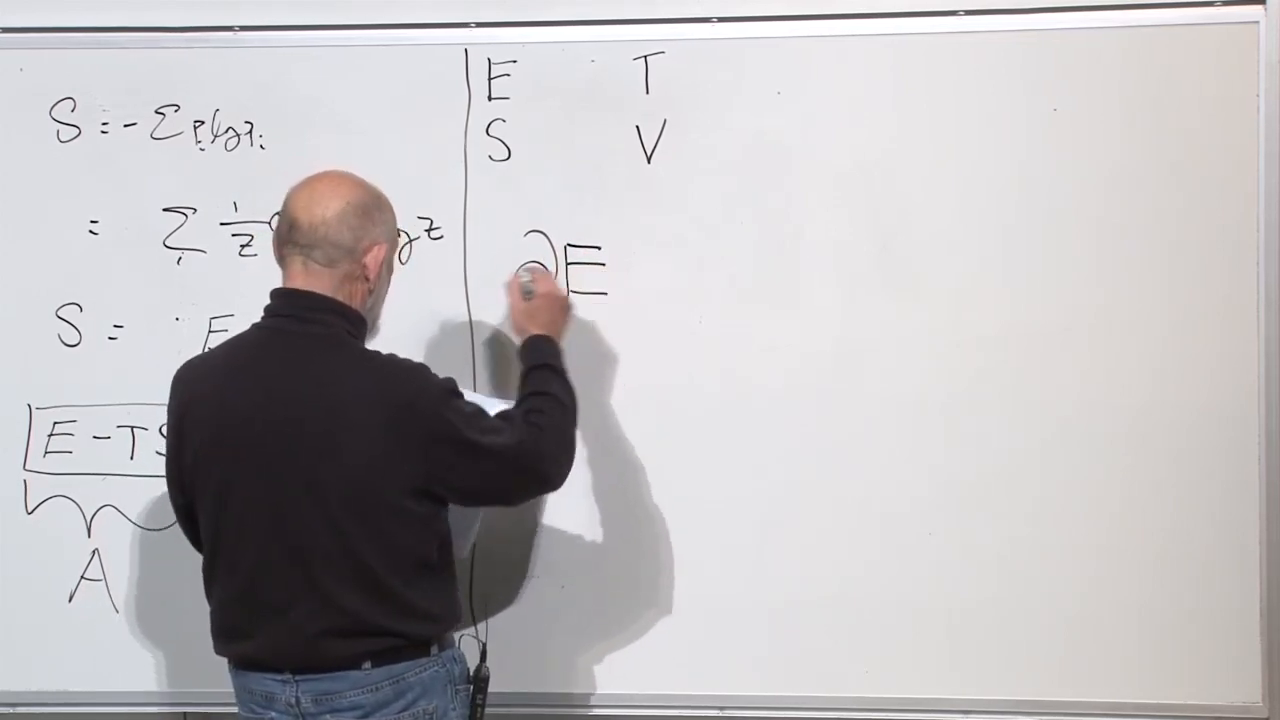
\includegraphics[width=0.90\textwidth]{lecture_05_figure_03.png}\caption{\(A=E-TS=-T\log Z\)}\lectureframe{00:16:50}\end{figure}

\section{Kontrollparameter und ihre Antworten}

Ein Kontrollparameter ist eine makroskopische Größe, die sich von außen durch einen Experimentator verändern lässt. Eine Verschiebung des Kolbens ändert das Volumen, ohne dass einzelne Moleküle manipuliert werden müssen. Angelegte elektrische und magnetische Felder sind weitere Beispiele. In einem allgemeineren Ensemble kann auch die Teilchenzahl variabel sein.

Thermodynamische Variablen treten natürlicherweise in konjugierten Paaren auf. Im vorliegenden Problem ist das Volumen der Kontrollparameter und der Druck seine Antwort. Wir verändern \(V\); der Druck gibt an, wie stark sich das System energetisch gegen diese Änderung wehrt. Später wird die Ableitung der Energie diese Paarung präzisieren.

\begin{classroomqa}\audiencequestion{Kann man den Druck selbst als Kontrollparameter auffassen?}\lecturerresponse{Man kann ein Experiment so gestalten, dass der äußere Druck festgelegt wird. Bei der hier betrachteten Anordnung legt jedoch die Kolbenposition das Volumen fest, und der Innendruck ist die Antwort des Systems. Druck und Volumen sind konjugierte Variablen; welche davon kontrolliert wird, hängt vom Ensemble und vom Versuchsaufbau ab.\lecturetimestamp{00:19:22--00:20:01}}\end{classroomqa}

\begin{classroomqa}\audiencequestion{Wird angenommen, dass alle Moleküle identisch sind, oder ist das Argument auf ein Gas beschränkt?}\lecturerresponse{Für das thermodynamische Argument ist keine solche Einschränkung nötig. Der Zylinder kann mehrere Teilchensorten, eine Flüssigkeit oder sogar einen komprimierten Festkörper enthalten. Erst nachdem die allgemeine Druckformel hergeleitet wurde, dient die Zustandssumme des idealen Gases als Spezialanwendung.\lecturetimestamp{00:20:02--00:20:39}}\end{classroomqa}

\begin{classroomqa}\audiencequestion{Könnte man die Stoffmenge durch einen weiteren äußeren Eingriff verändern?}\lecturerresponse{Ja. Die Teilchenzahl ist ein weiterer möglicher Kontrollparameter. Behandelt man sie als veränderlich, gehört dazu eine eigene konjugierte Variable: das chemische Potenzial. Für die Rechnung heute Abend bleibt \(N\) fest.\lecturetimestamp{00:20:39--00:20:57}}\end{classroomqa}

\begin{classroomqa}\audiencequestion{Können flüssiges Wasser und Dampf gleichzeitig im Gleichgewicht vorliegen?}\lecturerresponse{Bei der Koexistenztemperatur und dem Koexistenzdruck können sie das. Die Schwerkraft kann die Flüssigkeit unterhalb des Dampfes anordnen; dennoch können beide Phasen dieselbe Temperatur haben und sich im thermischen Gleichgewicht befinden. Derselbe allgemeine statistisch-mechanische Rahmen gilt auch hier.\lecturetimestamp{00:20:59--00:21:36}}\end{classroomqa}

Betrachten wir für das nächste Argument Energie und Entropie als abhängige Funktionen zweier unabhängig einstellbarer Variablen: \begin{equation}
 E=E(T,V),
 \qquad
 S=S(T,V).
 \label{eq:sm5-dependent-functions}
\end{equation}. Temperatur und Volumen bilden Koordinaten im thermodynamischen Zustandsraum. Energie und Entropie ordnen jedem Gleichgewichtspunkt in diesem Raum jeweils eine Zahl zu.

\section{Die Ableitung bei konstanter Entropie}

Die Ableitung, die wir letztlich benötigen, ist ungewöhnlich: \[
 \left(\frac{\partial E}{\partial V}\right)_S.
\]. Obwohl \(T\) und \(V\) die unabhängigen Koordinaten sind, wird bei dieser Ableitung \(V\) verändert, während die abhängige Funktion \(S(T,V)\) konstant gehalten wird. Es handelt sich um eine Ableitung entlang einer Kurve in der \((T,V)\)-Ebene, nicht entlang einer Koordinatenachse.

\begin{classroomqa}\audiencequestion{Wie können \(T\) und \(V\) unabhängig sein, wenn später die Ableitung \(dT/dV\) verwendet wird?}\lecturerresponse{Im gesamten Zustandsraum sind sie unabhängig. Sobald wir die Bedingung \(S(T,V)=\mathrm{constant}\) auferlegen, liegen die zulässigen Zustände auf einer eindimensionalen Kontur. Entlang dieser Kontur wird \(T\) zu einer Funktion von \(V\), und ihre Steigung \(dT/dV\) ist wohldefiniert.\lecturetimestamp{01:01:18--01:02:09}}\end{classroomqa}

\begin{lemma}Wenn \(E(T,V)\) und \(S(T,V)\) differenzierbar sind, gilt überall dort, wo \((\partial S/\partial T)_V\neq0\), \begin{equation}
 \left(\frac{\partial E}{\partial V}\right)_S
 =
 \left(\frac{\partial E}{\partial V}\right)_T
 -
 \left(\frac{\partial E}{\partial S}\right)_V
 \left(\frac{\partial S}{\partial V}\right)_T.
 \label{eq:sm5-calculus-lemma}
\end{equation}\end{lemma}

\begin{proof}Für eine beliebige infinitesimale Verschiebung gilt \begin{equation}
 dE=
 \left(\frac{\partial E}{\partial V}\right)_T dV
 +
 \left(\frac{\partial E}{\partial T}\right)_V dT.
 \label{eq:sm5-total-differential-e}
\end{equation}. Bei festem \(V\) erlaubt die Kettenregel, \(S\) als Zwischenvariable zu verwenden: \begin{equation}
 \left(\frac{\partial E}{\partial T}\right)_V
 =
 \left(\frac{\partial E}{\partial S}\right)_V
 \left(\frac{\partial S}{\partial T}\right)_V.
 \label{eq:sm5-chain-rule-e-s-t}
\end{equation}

Beschränken wir die Verschiebung nun auf eine Kontur, auf der \(S\) konstant ist. Entlang dieser Kontur gilt \begin{equation}
 0=dS=
 \left(\frac{\partial S}{\partial V}\right)_T dV
 +
 \left(\frac{\partial S}{\partial T}\right)_V dT.
 \label{eq:sm5-constant-entropy-differential}
\end{equation}. Auflösen nach der Steigung der Kontur ergibt \begin{equation}
 \left(\frac{dT}{dV}\right)_S
 =
 -
 \frac{\left(\frac{\partial S}{\partial V}\right)_T}
 {\left(\frac{\partial S}{\partial T}\right)_V}.
 \label{eq:sm5-entropy-contour-slope}
\end{equation}. Teilen wir \eqref{eq:sm5-total-differential-e} durch \(dV\), verwenden \eqref{eq:sm5-chain-rule-e-s-t} und setzen \eqref{eq:sm5-entropy-contour-slope} ein, so folgt \begin{align}
 \left(\frac{\partial E}{\partial V}\right)_S
 &=
 \left(\frac{\partial E}{\partial V}\right)_T
 +
 \left(\frac{\partial E}{\partial S}\right)_V
 \left(\frac{\partial S}{\partial T}\right)_V
 \left(\frac{dT}{dV}\right)_S \notag\\
 &=
 \left(\frac{\partial E}{\partial V}\right)_T
 -
 \left(\frac{\partial E}{\partial S}\right)_V
 \left(\frac{\partial S}{\partial V}\right)_T.
\end{align}. Der Faktor \((\partial S/\partial T)_V\) hat sich herausgekürzt; damit ist das Ergebnis bewiesen.\end{proof}

\begin{figure}[t]\centering
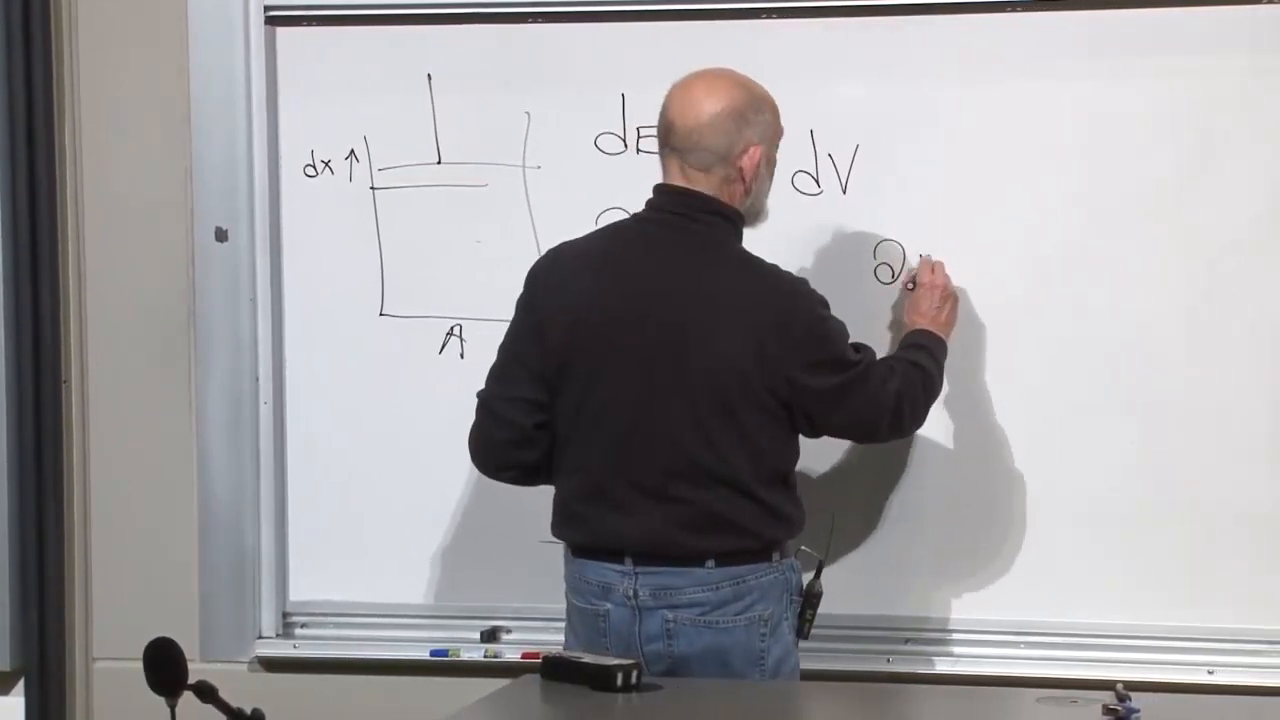
\includegraphics[width=0.90\textwidth]{lecture_05_figure_04.png}\caption{Die Berechnung entlang der Kontur konstanter Entropie an dem Punkt, an dem sich der Faktor herauskürzt und das Ableitungslemma damit bewiesen ist.}\lectureframe{00:36:10}\end{figure}

Das geometrische Bild ist keine bloße Zierde. Es erklärt, warum sich eine scheinbar ungewöhnliche Ableitung bei festem \(S\) mit gewöhnlichen partiellen Ableitungen nach den unabhängigen Koordinaten \(T\) und \(V\) berechnen lässt. Während der Herleitung \(\delta E/\delta V\) zu schreiben, erinnert daran, dass die Symbole Verhältnisse kleiner Änderungen entlang eines festgelegten Weges darstellen.

\begin{classroomqa}\audiencequestion{Ist die Entwicklung von \(dE\) einfach die übliche Definition partieller Ableitungen?}\lecturerresponse{Ja. Im totalen Differential ist nichts Besonderes enthalten. Hinzu kommt nur die spätere Einschränkung auf die Kontur \(dS=0\), die den Zusammenhang zwischen \(dT\) und \(dV\) festlegt.\lecturetimestamp{00:29:26--00:29:32}}\end{classroomqa}

\begin{classroomqa}\audiencequestion{Muss für die Kürzung \((\partial S/\partial T)_V\) von null verschieden sein?}\lecturerresponse{Ja. Für ein gewöhnliches stabiles System gilt \[
 \left(\frac{\partial S}{\partial T}\right)_V
 =\frac{C_V}{T}>0,
\], sodass die Division zulässig ist. In Ausnahmefällen ist eine gesonderte Betrachtung nötig. Bei festem Hamiltonoperator verbreitert eine Temperaturerhöhung die kanonische Energieverteilung und erhöht gewöhnlich die Entropie; eine Temperaturerniedrigung verengt sie. Das ist die physikalisch richtige Richtung des Monotoniearguments.\lecturetimestamp{00:36:50--00:37:47}}\end{classroomqa}

\section{Kolbenarbeit und adiabatische Bedingung}

Nun geben wir der Ableitung eine physikalische Bedeutung. Betrachten wir einen Kolben mit der Querschnittsfläche \(\mathcal A\). Bewegt er sich um \(dx\) nach außen, gilt \begin{equation}
 dV=\mathcal A\,dx.
 \label{eq:sm5-piston-volume}
\end{equation}. Das Gas übt die Kraft \(P\mathcal A\) auf den Kolben aus. Die vom Gas verrichtete Arbeit ist daher \begin{equation}
 \delta W_{\mathrm{by}}=P\mathcal A\,dx=P\,dV.
 \label{eq:sm5-piston-work}
\end{equation}. Tritt keine Wärme in das Gas ein, folgt aus der Energieerhaltung \begin{equation}
 dE=-P\,dV.
 \label{eq:sm5-adiabatic-work}
\end{equation}. Das Vorzeichen hat eine physikalische Bedeutung: Bei der Expansion hebt das Gas den Kolben an oder beschleunigt ihn, und seine eigene Energie nimmt ab.

\begin{figure}[t]\centering
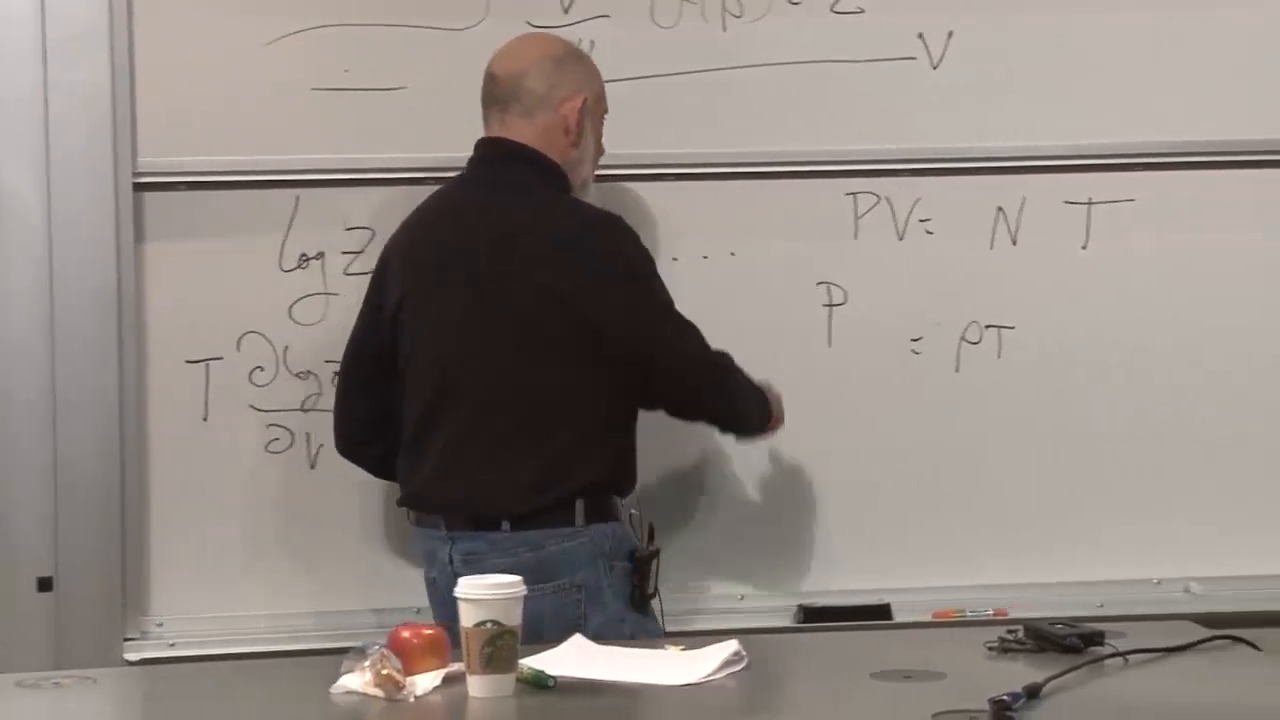
\includegraphics[width=0.90\textwidth]{lecture_05_figure_05.png}\caption{Die Geometrie des Kolbens und die vollständige Arbeitsbeziehung \(dE=-P\,dV\).}\lectureframe{00:43:10}\end{figure}

Zwei Einschränkungen sind wesentlich. Der Kolben muss sich langsam genug bewegen, damit das System beliebig nahe am Gleichgewicht bleibt, und die Wände müssen isoliert sein, damit keine Energie in Form von Wärme zugeführt wird. Ein schneller Zug kann so rasch erfolgen, dass während der Bewegung kein Molekül den zurückweichenden Kolben erreicht. Eine schnelle Kompression löst Stoßwellen aus. Keiner dieser Vorgänge lässt sich als Folge von Gleichgewichtszuständen darstellen.

Das Wort \emph{adiabatisch} wird bisweilen für fehlenden Wärmeaustausch und bisweilen für eine langsame Änderung verwendet. Beim hier erforderlichen reversiblen Vorgang spielen beide Bedeutungen eine Rolle: Die Änderung verläuft quasistatisch und das System ist thermisch isoliert. Unter diesen Bedingungen ist sie zugleich isentrop.

\begin{classroomqa}\audiencequestion{Warum bleibt die Entropie bei einer adiabatischen Änderung konstant?}\lecturerresponse{Betrachten wir das System quantenmechanisch. Seine Vielteilchenenergieniveaus hängen vom Volumen ab. Ändert sich \(V\) langsam, führt der adiabatische Satz jedes besetzte Niveau stetig in sein Nachfolgeniveau über, ohne Übergänge zwischen den Niveauindizes. Die Energien \(E_i(V)\) ändern sich, die Besetzungswahrscheinlichkeiten \(p_i\) bleiben jedoch unverändert. Da \(S=-\sum_i p_i\log p_i\) von diesen Wahrscheinlichkeiten abhängt, bleibt auch die Entropie konstant. Wärmeaustausch oder irreversible Bewegung würden diese Schlussfolgerung ungültig machen.\lecturetimestamp{00:43:37--00:49:15}}\end{classroomqa}

\begin{figure}[t]\centering
\includegraphics[width=0.90\textwidth]{lecture_05_figure_06.png}\caption{Vielteilchenenergieniveaus verschieben sich mit dem Volumen, während ihre Besetzungswahrscheinlichkeiten den jeweiligen Niveauindizes zugeordnet bleiben.}\lectureframe{00:48:50}\end{figure}

Gleichung \eqref{eq:sm5-adiabatic-work}, ausgewertet entlang dieses Weges konstanter Entropie, weist den Druck aus als \begin{equation}
 P=-\left(\frac{\partial E}{\partial V}\right)_S.
 \label{eq:sm5-pressure-fixed-entropy}
\end{equation}. Das ist die konjugierte Beziehung zwischen Druck und Volumen.

\begin{classroomqa}\audiencequestion{Was passiert, wenn der Kolben stattdessen schnell bewegt wird?}\lecturerresponse{Das System verlässt das Gleichgewicht, und seine detaillierte Dynamik wird wichtig. Eine plötzliche Kompression erzeugt einen Stoß. Bei einer idealen freien Expansion kann sich der Kolben zurückziehen, bevor ihn ein Molekül trifft; dann wird keine Arbeit verrichtet und die Energie bleibt konstant, obwohl sich das Volumen ändert. Das Gas stellt später unter Zunahme der Entropie das Gleichgewicht wieder her. Solche Vorgänge lassen sich nicht mit der einzelnen Gleichgewichtsableitung in \eqref{eq:sm5-pressure-fixed-entropy} beschreiben.\lecturetimestamp{00:58:30--01:01:15}}\end{classroomqa}

\begin{classroomqa}\audiencequestion{Welche quantitative Bedingung entscheidet, ob eine Änderung langsam ist?}\lecturerresponse{Die Zeit, über die sich die äußeren Bedingungen ändern, muss groß sein im Vergleich zu den relevanten inneren Relaxationszeiten. Bei einem Gas sollten während der makroskopischen Änderung viele Molekülstöße und viele Stöße gegen die Wände stattfinden. Die genaue Zeitskala hängt vom Material und von der Geometrie ab; der quasistatische Grenzfall ist dagegen allgemein.\lecturetimestamp{01:02:09--01:03:20}}\end{classroomqa}

\section{Von der adiabatischen Energie zur Zustandssumme}

Die physikalische Formel \eqref{eq:sm5-pressure-fixed-entropy} ist noch nicht diejenige, die sich am einfachsten berechnen lässt. Die kanonische statistische Mechanik liefert auf natürliche Weise Funktionen der Temperatur, denn \(T\) tritt unmittelbar im Boltzmann-Faktor auf. Das Analysislemma überführt die unhandliche Ableitung bei konstanter Entropie in diese für Berechnungen geeignete Form: \begin{align}
 P
 &=
 -\left(\frac{\partial E}{\partial V}\right)_T
 +
 \left(\frac{\partial E}{\partial S}\right)_V
 \left(\frac{\partial S}{\partial V}\right)_T.
 \label{eq:sm5-pressure-lemma-substitution}
\end{align}. Bei festem Volumen liefert der erste Hauptsatz \(dE=T\,dS\) und damit \begin{equation}
 \left(\frac{\partial E}{\partial S}\right)_V=T.
 \label{eq:sm5-e-s-temperature}
\end{equation}. Somit gilt \begin{equation}
 P=
 -\left(\frac{\partial E}{\partial V}\right)_T
 +
 T\left(\frac{\partial S}{\partial V}\right)_T.
 \label{eq:sm5-pressure-fixed-temperature-pieces}
\end{equation}

\begin{classroomqa}\audiencequestion{Woher kommt das Minuszeichen in der Druckformel?}\lecturerresponse{Es stammt aus der vom Gas verrichteten Arbeit: \(dE=-P\,dV\) bei adiabatischer Expansion. Das Analysislemma selbst enthält zwischen seinen beiden Termen ein Minuszeichen; das vorangestellte Minus in \(P=-(\partial E/\partial V)_S\) kehrt beide Terme um und ergibt \eqref{eq:sm5-pressure-fixed-temperature-pieces}.\lecturetimestamp{00:52:40--00:53:14}}\end{classroomqa}

Da \(T\) in beiden Ableitungen festgehalten wird, gilt \begin{align}
 P
 &=
 -\left(\frac{\partial}{\partial V}(E-TS)\right)_T \notag\\
 &=
 -\left(\frac{\partial A}{\partial V}\right)_T.
 \label{eq:sm5-pressure-free-energy}
\end{align}. Schließlich setzen wir \(A=-T\log Z\) ein: \begin{equation}
 \boxed{
 P=
 T\left(\frac{\partial\log Z}{\partial V}\right)_T
 }.
 \label{eq:sm5-pressure-log-z}
\end{equation}

\begin{figure}[t]\centering
\includegraphics[width=0.90\textwidth]{lecture_05_figure_07.png}\caption{Die Umformung bei fester Temperatur: \(P=-(\partial A/\partial V)_T
=T(\partial\log Z/\partial V)_T\).}\lectureframe{00:55:55}\end{figure}

In \eqref{eq:sm5-pressure-log-z} wird kein ideales Gas vorausgesetzt. Lässt sich die Zustandssumme einer wechselwirkenden Flüssigkeit, eines Plasmas oder eines Festkörpers berechnen, liefert dieselbe Ableitung dessen Druck. Allgemeiner erhält man zu jedem äußeren Kontrollparameter eine konjugierte Antwortgröße, indem man ein geeignetes thermodynamisches Potenzial ableitet. Die Zustandssumme fasst viele solcher Antworten zusammen: Ableiten von \(\log Z\) nach \(\beta\) ergibt die Energie, Ableiten nach dem Volumen den Druck.

\section{Die Zustandsgleichung des idealen Gases}

Erst jetzt spezialisieren wir auf \(N\) nicht wechselwirkende Teilchen. Unter Beibehaltung der klassischen Normierung des Phasenraums gilt \begin{equation}
 Z_N=
 \frac{1}{N!h^{3N}}
 \int d^{3N}q\,d^{3N}p\,
 \exp\!\left[
 -\beta\sum_{a=1}^{N}\frac{\mathbf p_a^2}{2m}
 \right].
 \label{eq:sm5-ideal-gas-partition-integral}
\end{equation}. Es gibt \(3N\) Ortskoordinaten und \(3N\) Impulskoordinaten. Der Hamiltonoperator hängt nicht vom Ort ab, daher liefert jedes Teilchen einen Faktor, der dem Behältervolumen entspricht: \begin{equation}
 Z_N=
 \frac{V^N}{N!h^{3N}}I_p(\beta),
 \label{eq:sm5-ideal-gas-factorization}
\end{equation}, wobei das gesamte Impulsintegral \(I_p(\beta)\) unabhängig von \(V\) ist.

\begin{classroomqa}\audiencequestion{Warum gibt es \(3N\) Ortsintegrale und \(3N\) Impulsintegrale?}\lecturerresponse{Jedes der \(N\) Teilchen hat drei räumliche Koordinaten und drei konjugierte Impulskomponenten. Die Anzahl beträgt \(3N\) in jeder Hälfte des Phasenraums, nicht \(N\) Teilchen plus weitere \(3N\) Teilchen.\lecturetimestamp{01:04:19--01:04:28}}\end{classroomqa}

Ein Logarithmus trennt die Volumenabhängigkeit ab: \begin{equation}
 \log Z_N
 =
 N\log V-\log N!-3N\log h+\log I_p(\beta).
 \label{eq:sm5-log-ideal-gas-partition}
\end{equation}. Die Faktoren \(1/N!\), \(h^{-3N}\) und \(I_p(\beta)\) sind sämtlich unabhängig vom Volumen. Sie sind für die absolute Entropie und andere Fragestellungen wichtig, nicht jedoch für diese spezielle Ableitung. Daher gilt \begin{equation}
 \left(\frac{\partial\log Z_N}{\partial V}\right)_T
 =\frac{N}{V}.
 \label{eq:sm5-log-z-volume-derivative}
\end{equation}. Aus Gleichung \eqref{eq:sm5-pressure-log-z} folgt unmittelbar \begin{equation}
 P=\frac{NT}{V},
 \qquad
 \boxed{PV=NT}.
 \label{eq:sm5-ideal-gas-law}
\end{equation}

\begin{classroomqa}\audiencequestion{Zählt \(N\) weiterhin die Replikate mit, die zur Herleitung der Boltzmann-Verteilung verwendet wurden?}\lecturerresponse{Nein. Die Replikatkonstruktion war in der früheren Herleitung ein Hilfsmittel zum Zählen und kommt hier nicht mehr vor. Hier bezeichnet \(N\) die Anzahl der physikalischen Teilchen in dieser einzelnen Gasprobe.\lecturetimestamp{01:07:38--01:08:05}}\end{classroomqa}

Definieren wir die Teilchenzahldichte durch \begin{equation}
 \rho=\frac{N}{V}
 \label{eq:sm5-number-density}
\end{equation}, erhalten wir die äquivalente Form \begin{equation}
 P=\rho T.
 \label{eq:sm5-density-equation-of-state}
\end{equation}

\begin{classroomqa}\audiencequestion{Sollte man für die Dichteform durch \(N\) oder durch \(V\) dividieren?}\lecturerresponse{Dividiere \(PV=NT\) durch \(V\): \(P=(N/V)T=\rho T\). Hier bezeichnet \(\rho\) die Teilchenzahldichte, nicht die Massendichte.\lecturetimestamp{01:08:45--01:09:16}}\end{classroomqa}

\begin{figure}[t]\centering
\includegraphics[width=0.90\textwidth]{lecture_05_figure_08.png}\caption{Die Ableitung von \(\log Z\) nach dem Volumen und die daraus folgende Zustandsgleichung des idealen Gases \(PV=NT\) oder \(P=\rho T\).}\lectureframe{01:09:25}\end{figure}

Stellen wir die Labortemperatur \(T_K\) wieder her, so gilt \begin{equation}
 PV=Nk_BT_K.
 \label{eq:sm5-ideal-gas-law-laboratory}
\end{equation}. Das vertraute Ergebnis stimmt mit der kinetischen Intuition überein; seine Herleitung beruht nun aber auf einem Rahmen, der weit über das freie Gas hinaus Bestand hat.

\section{Ein weiterer Ertrag: Fluktuationen im Gleichgewicht}

Die Druckberechnung ist abgeschlossen, doch eine angekündigte Frage bleibt offen: Was lässt sich noch aus der Zustandssumme gewinnen? Betrachten wir ein System in thermischem Kontakt mit einem Wärmebad. Seine Energie ist nicht fest. Energie tritt ein und aus, sodass wiederholte Messungen um den kanonischen Mittelwert fluktuieren.

\begin{classroomqa}\audiencequestion{Können wir nun die angekündigten Fluktuationen berechnen?}\lecturerresponse{Ja. Die zusätzliche Zeit erlaubt eine zweite Demonstration desselben Prinzips: Ableitungen von \(Z\) enthalten messbare thermodynamische Information.\lecturetimestamp{01:10:37--01:10:50}}\end{classroomqa}

\subsection{Varianz und Standardabweichung}

Für eine Zufallsvariable \(x\) mit \(\langle x\rangle=0\) ist \(\langle x^2\rangle\) ein Maß für die Breite der Verteilung. Bei einer allgemeinen Verteilung verschieben wir die Variable um ihren Mittelwert: \begin{equation}
 \delta x=x-\langle x\rangle.
 \label{eq:sm5-centered-variable}
\end{equation}. Ihr Mittelwert ist null: \begin{equation}
 \langle\delta x\rangle
 =
 \langle x\rangle-\langle x\rangle=0,
 \label{eq:sm5-centered-mean}
\end{equation}, und ihr mittleres Quadrat ist \begin{align}
 (\Delta x)^2
 &\equiv
 \left\langle\left(x-\langle x\rangle\right)^2\right\rangle \notag\\
 &=
 \langle x^2\rangle
 -2\langle x\rangle^2
 +\langle x\rangle^2 \notag\\
 &=
 \langle x^2\rangle-\langle x\rangle^2.
 \label{eq:sm5-variance}
\end{align}. Das ist die Varianz. Ihre positive Quadratwurzel \(\Delta x\) ist die Standardabweichung.

\begin{classroomqa}\audiencequestion{Warum ist der Mittelwert von \(x-\langle x\rangle\) genau null?}\lecturerresponse{Mittelwerte sind linear, und \(\langle x\rangle\) ist bereits eine Zahl. Daher gilt \(\langle x-\langle x\rangle\rangle
=\langle x\rangle-\langle x\rangle=0\).\lecturetimestamp{01:14:02--01:14:22}}\end{classroomqa}

\begin{classroomqa}\audiencequestion{Was ist der Unterschied zwischen der quadrierten Fluktuation, der Varianz, der quadratischen Mittelwertbreite und der Standardabweichung?}\lecturerresponse{Die Varianz ist \((\Delta x)^2=\langle x^2\rangle-\langle x\rangle^2\). Ihre Quadratwurzel ist die Standardabweichung \(\Delta x\). Bei einer Zufallsvariable mit Mittelwert null ist die Standardabweichung zugleich ihr quadratischer Mittelwert.\lecturetimestamp{01:16:39--01:18:38}}\end{classroomqa}

\begin{figure}[t]\centering
\includegraphics[width=0.90\textwidth]{lecture_05_figure_09.png}\caption{Die verschobene Variable und die Entwicklung, aus der \((\Delta x)^2=\langle x^2\rangle-\langle x\rangle^2\) hervorgeht.}\lectureframe{01:17:20}\end{figure}

\subsection{Energiemomente aus der Zustandssumme}

Für das kanonische Ensemble gilt \begin{align}
 \langle E\rangle
 &=
 \frac{1}{Z}\sum_i E_i e^{-\beta E_i} \notag\\
 &=
 -\frac{1}{Z}\frac{\partial Z}{\partial\beta}
 =
 -\frac{\partial\log Z}{\partial\beta}.
 \label{eq:sm5-mean-energy-from-z}
\end{align}. Ein Faktor \(E_i\) wird durch eine negative Ableitung nach \(\beta\) erzeugt. Eine zweite Ableitung liefert \(E_i^2\): \begin{equation}
 \langle E^2\rangle
 =
 \frac{1}{Z}\sum_i E_i^2e^{-\beta E_i}
 =
 \frac{1}{Z}\frac{\partial^2 Z}{\partial\beta^2}.
 \label{eq:sm5-second-energy-moment}
\end{equation}. Damit ergibt sich für die Energievarianz \begin{align}
 (\Delta E)^2
 &=
 \langle E^2\rangle-\langle E\rangle^2 \notag\\
 &=
 \frac{1}{Z}\frac{\partial^2Z}{\partial\beta^2}
 -
 \frac{1}{Z^2}
 \left(\frac{\partial Z}{\partial\beta}\right)^2 \notag\\
 &=
 \frac{\partial^2\log Z}{\partial\beta^2}
 =
 -\frac{\partial\langle E\rangle}{\partial\beta}.
 \label{eq:sm5-energy-variance-beta}
\end{align}. Wieder wird eine kompliziert wirkende Observable zu einer Ableitung von \(\log Z\).

\begin{figure}[t]\centering
\includegraphics[width=0.90\textwidth]{lecture_05_figure_10.png}\caption{Die zweite Ableitung von \(\beta\) nach \(\log Z\), die mit der Energievarianz identifiziert wird.}\lectureframe{01:29:00}\end{figure}

\subsection{Wärmekapazität und Größe der Fluktuationen}

In den Einheiten der Vorlesung gilt \(T=1/\beta\), also \begin{equation}
 -\frac{\partial}{\partial\beta}
 =
 T^2\frac{\partial}{\partial T}.
 \label{eq:sm5-beta-temperature-derivative}
\end{equation}. Bei festem Volumen definieren wir die Wärmekapazität der gesamten Probe durch \begin{equation}
 C_V\equiv
 \left(\frac{\partial\langle E\rangle}{\partial T}\right)_V.
 \label{eq:sm5-heat-capacity}
\end{equation}. Aus Gleichung \eqref{eq:sm5-energy-variance-beta} wird \begin{equation}
 \boxed{(\Delta E)^2=T^2C_V}
 \qquad (k_B=1).
 \label{eq:sm5-energy-fluctuation-lecture-units}
\end{equation}. Für die Labortemperatur \(T_K\), für die \(\beta=(k_BT_K)^{-1}\) gilt, erhalten wir \begin{equation}
 \boxed{(\Delta E)^2=k_BT_K^2C_V}.
 \label{eq:sm5-energy-fluctuation-laboratory}
\end{equation}

\begin{figure}[t]\centering
\includegraphics[width=0.90\textwidth]{lecture_05_figure_11.png}\caption{Der Übergang von der Ableitung nach \(\beta\) zur Wärmekapazität bei festem Volumen, einschließlich des wieder eingesetzten Faktors \(k_B\).}\lectureframe{01:31:10}\end{figure}

\begin{classroomqa}\audiencequestion{Muss in der Ableitung das Volumen statt des Drucks als konstant festgelegt werden?}\lecturerresponse{Ja. Bei dieser kanonischen Herleitung bleiben die äußeren Kontrollparameter des Hamiltonoperators fest, einschließlich \(V\). Die resultierende Größe ist \(C_V\). In einem Ensemble bei konstantem Druck können Volumen und Arbeit fluktuieren; dafür wird das entsprechende thermodynamische Potenzial benötigt. Man kann \(C_V\) in \eqref{eq:sm5-energy-fluctuation-laboratory} nicht einfach durch \(C_P\) ersetzen.\lecturetimestamp{01:29:01--01:29:28; 01:32:50--01:33:21}}\end{classroomqa}

\begin{classroomqa}\audiencequestion{Ist \(C_V\) eine Materialkonstante?}\lecturerresponse{Im Allgemeinen nicht. Sie kann von Temperatur, Volumen, Phase und Zusammensetzung abhängen. Außerdem ist \(C_V\) hier die Wärmekapazität der gesamten Probe und damit eine extensive Größe. Eine spezifische Wärmekapazität erhält man erst, wenn man durch die Masse, die Teilchenzahl oder die Stoffmenge dividiert.\lecturetimestamp{01:31:47--01:32:21; 01:33:23--01:34:55}}\end{classroomqa}

Für gewöhnliche extensive Materie ist \(C_V\) proportional zu \(N\); daher ist \((\Delta E)^2\) proportional zu \(N\) und \(\Delta E\) proportional zu \(\sqrt{N}\). Die mittlere Energie selbst ist proportional zu \(N\). Folglich gilt \begin{equation}
 \frac{\Delta E}{\langle E\rangle}\sim\frac{1}{\sqrt{N}}.
 \label{eq:sm5-relative-fluctuation-scaling}
\end{equation}. Die relativen Fluktuationen sind bei makroskopischen Systemen winzig, während sie sich in mikroskopischen Proben direkt zeigen. Das Auftreten von \(k_B\) in \eqref{eq:sm5-energy-fluctuation-laboratory} kennzeichnet diesen Zusammenhang zwischen thermodynamischen Observablen und der Diskretheit auf Molekülebene; gleichwertig verbindet es makroskopische Einheiten mit Zählungen auf der Avogadro-Skala.

Druck und Fluktuationen sind nun aus derselben Größe hervorgegangen: \[
 P=T\left(\frac{\partial\log Z}{\partial V}\right)_T,
 \qquad
 (\Delta E)^2=\frac{\partial^2\log Z}{\partial\beta^2}.
\]. Das ist die zentrale Erkenntnis. Sobald die richtigen Zwangsbedingungen bestimmt sind, dient die Zustandssumme nicht nur der Normierung von Wahrscheinlichkeiten. Ihre Ableitungen ordnen die messbare Thermodynamik des Systems.
\chapter{Schwache Wechselwirkungen, Virialkorrekturen und unexakte Differentiale}

\lectureoverview{Wir beginnen mit der operationalen Bedeutung von Messung und Temperatur und fragen dann, wie ein verdünntes Gas vom idealen Gasgesetz abweicht, wenn schwache Wechselwirkungen kurzer Reichweite eingeschaltet werden. Die Zustandssumme liefert die ersten Wechselwirkungskorrekturen zu Energie und Druck und gibt ihren Gültigkeitsbereich an. Ein abschließender mathematischer Exkurs unterscheidet Zustandsfunktionen von wegabhängiger Wärme und Arbeit mithilfe exakter Differentiale, geschlossener Wege und eines konkreten Tests am idealen Gas.}

\section{Was ein Messgerät tatsächlich misst}

Kein Laborgerät greift unmittelbar auf die Natur zu und gibt eine abstrakte mathematische Variable aus. Eine Federwaage zeigt eine Auslenkung an, ein Thermometer die Höhe einer Flüssigkeitssäule. Wir bezeichnen das eine als Kraftmessung und das andere als Temperaturmessung, weil eine reproduzierbare Beziehung zwischen der sichtbaren Anzeige und der gesuchten Größe hergestellt wurde.

Diese Beziehung gilt nur in einem begrenzten Bereich. Eine Feder folgt dem Hookeschen Gesetz nur, solange sie elastisch bleibt; bei hinreichend großer Kraft verformt sie sich schließlich oder bricht. Allgemeiner gilt: Wenn eine glatte Anzeige \(R\) von einer physikalischen Variablen \(X\) abhängt, dann gilt in der Nähe eines gewählten Arbeitspunkts
\begin{equation}
 \Delta R \simeq
 \left.\frac{dR}{dX}\right|_{X_0}\Delta X.
 \label{eq:sm6-local-linear-response}
\end{equation}
Kleine Änderungen der Anzeige sind proportional zu kleinen Änderungen der Zielgröße, auch wenn die gesamte Kennlinie nichtlinear ist. Diese lokale Linearisierung ist die übliche Grundlage der Kalibrierung.

Die Anzeige kann auch von Störgrößen abhängen. Eine Feder kann schwach auf Temperatur oder Druck reagieren. Die Höhe des Quecksilbers in einem Thermometer könnte sich durch die Orientierung infolge der Schwerkraft, durch Eigenschaften des Glases oder durch langsame Veränderungen der Materialien ändern. Ein Messverfahren beweist nicht, dass solche Abhängigkeiten fehlen; es hält sie konstant oder zeigt, dass sie auf der benötigten Skala vernachlässigbar sind.

\begin{classroomqa}
\audiencequestion{Könnten das lokale Gravitationsfeld oder die Richtung, in der das Thermometer gehalten wird, die Anzeige verändern?}
\lecturerresponse{Ja, grundsätzlich. Wenn die Orientierung einen merklichen Einfluss hat, gehört die Anweisung, das Thermometer senkrecht zu halten, zur Definition des Messgeräts. Nahe der Erdoberfläche ist das Gravitationsfeld hinreichend stabil, sodass die verbleibenden Schwankungen normalerweise vernachlässigbar sind.
\lecturetimestamp{00:04:08--00:05:00}}
\end{classroomqa}

\begin{classroomqa}
\audiencequestion{Können Alterung oder chemische Veränderungen die Kalibrierung allmählich verändern?}
\lecturerresponse{Das ist möglich. Quecksilber und Glas sind für gewöhnliche Messungen hinreichend inert; Veränderungen auf unglaublich langen Zeitskalen sind für das Experiment unerheblich. Eine Kalibrierung gilt immer für ein bestimmtes Messgerät, einen bestimmten Bereich, ein bestimmtes Verfahren und eine bestimmte Dauer.
\lecturetimestamp{00:05:03--00:06:11}}
\end{classroomqa}

Bei einem Celsius-Thermometer liefern zwei reproduzierbare Referenzzustände eine praktische Skala. Sind \(h_f\) und \(h_b\) die Säulenhöhen an den Gefrier- beziehungsweise Siedepunkten von Wasser, so gilt in einem Bereich, in dem die Anzeige annähernd linear ist,
\begin{equation}
 T_{\mathrm C}=100\,\frac{h-h_f}{h_b-h_f}.
 \label{eq:sm6-celsius-calibration}
\end{equation}
Die Festlegung \(T_{\mathrm C}=0\) am Gefrierpunkt ist eine Konvention. Sie bezeichnet nicht den Zustand mit null thermischer Energie, genauso wenig wie null Grad Fahrenheit an einem Wintertag den absoluten Nullpunkt bezeichnet.

\begin{figure}[t]
\centering
\includegraphics[width=0.90\textwidth]{lecture_06_figure_03.png}
\caption{Glatter, aber nichtlinearer Verlauf der Thermometeranzeige mit einem kurzen, für die lineare Kalibrierung markierten Abschnitt.}
\lectureframe{00:07:55}
\end{figure}

\section{Gleichgewicht und Temperatur als Energieskala}

Ein Thermometer misst die Temperatur seiner Umgebung erst, wenn es mit dem angrenzenden Medium das thermische Gleichgewicht erreicht hat. Bis dahin ändert sich seine Anzeige lediglich in Richtung des Gleichgewichts. Der praktische Test ist einfach: Man wartet, bis sich die Anzeige nicht mehr ändert. Hinter dieser einfachen Regel stehen physikalische Prozesse, die die Wartezeit bestimmen.

\begin{classroomqa}
\audiencequestion{Findet der Ausgleich nur in einer Grenzschicht um den Kolben statt, und wie lange sollte man warten?}
\lecturerresponse{Energie muss das Glas durchqueren und mit dem umgebenden Medium ausgetauscht werden. Die benötigte Zeit hängt daher vom Thermometer, seiner Wärmeleitfähigkeit und dem Medium ab. Auch die unmittelbare Umgebung muss für einen homogenen Gleichgewichtszustand repräsentativ sein. Im Experiment gilt die Anzeige als stabil, wenn sie nicht mehr driftet.
\lecturetimestamp{00:08:45--00:10:13}}
\end{classroomqa}

Temperatur und Dichte spielen bei dieser Wartezeit unterschiedliche Rollen. Ein sehr verdünntes Gas kann sehr heiß sein: Die wenigen vorhandenen Moleküle können große kinetische Energien tragen. Sie stoßen jedoch nur selten mit dem Thermometer zusammen, sodass der Temperaturausgleich langsam sein kann. Eine Verringerung der Dichte um den Faktor einhundert oder tausend bei gleichbleibender Temperatur senkt nicht die molekulare Energieskala; sie verringert die Rate, mit der diese Energie an das Messgerät übertragen wird.

\begin{classroomqa}
\audiencequestion{Kann die Strahlung in einem Raum eine andere Temperatur haben als die Luft?}
\lecturerresponse{Ja. Materie und Strahlung haben nur dann dieselbe Temperatur, wenn sie miteinander im thermischen Gleichgewicht sind. Neutrale Luft koppelt nur schwach an einen großen Teil der optischen Strahlung in einem beleuchteten Raum; die Photonenzahlverteilung muss daher kein Gleichgewichts-Schwarzkörperfeld mit der Lufttemperatur sein.
\lecturetimestamp{00:11:26--00:12:20}}
\end{classroomqa}

Ist das Gleichgewicht erreicht, betrachtet man die Temperatur am besten als Energieskala. Wir verwenden weiterhin Einheiten mit \(k_B=1\), sodass \(T\) selbst die Dimension einer Energie hat. Für ein einatomiges ideales Gas gilt
\begin{equation}
 E_0=\frac{3}{2}NT.
 \label{eq:sm6-ideal-energy}
\end{equation}
Die thermische Energie pro Molekül wird durch \(T\) festgelegt; die zugehörige Geschwindigkeit hängt weiterhin von der Molekülmasse ab.

\section{Eine schwache Wechselwirkung einschalten}

\begin{classroomqa}
\audiencequestion{Unter welchen Bedingungen versagt die Näherung des idealen Gases, und lässt sich dieses Versagen mathematisch zeigen?}
\lecturerresponse{Man geht vom gelösten wechselwirkungsfreien Gas aus und schaltet eine kleine Wechselwirkung ein. Man entwickelt nach dieser Änderung, berechnet die erste Korrektur und vergleicht sie mit dem idealen Beitrag. Die Näherung versagt, wenn die Korrektur nicht mehr klein ist.
\lecturetimestamp{00:12:25--00:14:40}}
\end{classroomqa}

Das ist die übliche Störungsstrategie. Ist ein Problem für \(\lambda=0\) lösbar, führt man eine Kopplung \(\lambda\) ein, schreibt
\begin{equation}
 F(\lambda)=F(0)+\lambda F_1+\lambda^2F_2+\cdots,
 \label{eq:sm6-perturbative-template}
\end{equation}
und prüft, ob jeder berücksichtigte Term kleiner ist als der vorhergehende. Hier ist das Referenzproblem das ideale Gas. Die physikalische Kleinheit beruht auf einer verdünnten Probe, einer kurzen Wechselwirkungsreichweite im Vergleich zum mittleren Teilchenabstand und einem hinreichend schwachen Potential, sodass der erste Wechselwirkungsterm brauchbar ist. Hohe Dichte oder eine langreichweitige Kraft können die Näherung ungültig machen, selbst wenn jede einzelne Begegnung harmlos erscheint.

Seien \(x_i\in\mathbb R^3\) und \(p_i\in\mathbb R^3\) Ort und Impuls des Moleküls \(i\). Für identische Moleküle der Masse \(m\) setzen wir
\begin{equation}
 H(X,P)=
 \sum_{i=1}^{N}\frac{p_i^2}{2m}
 +\sum_{i<j}u\!\left(|x_i-x_j|\right),
 \label{eq:sm6-interacting-hamiltonian}
\end{equation}
wobei \(X=(x_1,\ldots,x_N)\) und \(P=(p_1,\ldots,p_N)\). Die Einschränkung \(i<j\) schließt Selbstpaare aus und zählt \((i,j)\) nur einmal:
\begin{equation}
 \sum_{i<j}1=\binom{N}{2}=\frac{N(N-1)}{2}.
 \label{eq:sm6-pair-count}
\end{equation}

\begin{classroomqa}
\audiencequestion{Warum summiert man nicht unabhängig über beide Teilchenindizes?}
\lecturerresponse{Das Paar \((3,7)\) ist dasselbe physikalische Paar wie \((7,3)\), und ein Teilchen bildet kein Paar mit sich selbst. Die Beschränkung auf \(i<j\) berücksichtigt beides. Das Massensymbol bleibt \(m\), während \(i,j\) die Teilchen kennzeichnen, um den möglichen Notationskonflikt zu vermeiden, wenn \(m\) für beide Zwecke verwendet wird.
\lecturetimestamp{00:17:52--00:19:12}}
\end{classroomqa}

Das gesamte Konfigurationspotential schreiben wir als
\begin{equation}
 U(X)=\sum_{i<j}u\!\left(|x_i-x_j|\right).
 \label{eq:sm6-total-potential}
\end{equation}
Die Wechselwirkung wird als translationsinvariant und kurzreichweitig angenommen: \(u(r)\) wird vernachlässigbar, wenn \(r\) groß gegenüber einer molekularen Längenskala ist.

\section{Die integrierte Paarwechselwirkung}

In die erste Korrektur geht nur ein Integral des schwachen Paarpotentials ein:
\begin{equation}
 U_0\equiv\int_{\mathbb R^3}d^3r\,u(r).
 \label{eq:sm6-u0-definition}
\end{equation}
Seine Einheit ist Energie mal Volumen. Es verbindet die typische Stärke der Wechselwirkung mit dem Volumen, über das diese Wechselwirkung merklich ist.

\begin{figure}[t]
\centering
\includegraphics[width=0.90\textwidth]{lecture_06_figure_04.png}
\caption{Das kurzreichweitige Paarpotential, zusammengefasst in der integrierten Stärke \(U_0=\int d^3r\,u(r)\).}
\lectureframe{00:25:15}
\end{figure}

Um zu sehen, warum \(U_0\) nützlich ist, betrachten wir ein Teilchenpaar:
\begin{equation}
 I_2=\int_V d^3x_1\,d^3x_2\,
 u\!\left(|x_1-x_2|\right).
 \label{eq:sm6-two-particle-integral}
\end{equation}
Wir führen eine Relativkoordinate \(r=x_2-x_1\) ein. Abseits des Randes liefert das Relativintegral \(U_0\), während sich die gemeinsame Position des Paares über den gesamten Behälter erstreckt. Somit gilt
\begin{equation}
 I_2=V U_0+\text{surface corrections}.
 \label{eq:sm6-pair-integral-vu0}
\end{equation}
Die Korrektur stammt von Teilchen, die höchstens eine Wechselwirkungsreichweite von der Wand entfernt sind. Dort liegt ein Teil der Umgebung in der Relativkoordinate außerhalb des Behälters. Ihr relativer Beitrag skaliert wie das Verhältnis von Oberfläche zu Volumen und verschwindet im makroskopischen Grenzfall.

\begin{classroomqa}
\audiencequestion{Bezieht sich \(U_0\) auf ein ausgewähltes Paar, und wird ein Teilchen in festem Abstand zum anderen gehalten?}
\lecturerresponse{Gemeint ist das gemeinsame Wechselwirkungsgesetz für ein beliebiges Paar. Man hält das erste Teilchen fest und integriert über alle Relativpositionen des zweiten. Der Abstand bleibt während dieses Integrals nicht konstant. Einen merklichen Beitrag liefert nur der nahe Wechselwirkungsbereich; daraus ergibt sich \(U_0\).
\lecturetimestamp{00:26:03--00:27:33}}
\end{classroomqa}

\begin{classroomqa}
\audiencequestion{Warum ergibt das Positionsintegral über das zweite Teilchen das volle Behältervolumen, das über das erste aber nicht?}
\lecturerresponse{Nachdem die Relativkonfiguration in \(U_0\) integriert wurde, lässt sich das ganze Paar durch die Probe verschieben. Diese gemeinsame Translation liefert den großen Faktor \(V\). Die Wechselwirkungsumgebung hat ein Volumen auf molekularer Skala und ist bereits in \(U_0\) enthalten; sie liefert keinen weiteren Faktor, der dem Behältervolumen entspricht.
\lecturetimestamp{00:27:48--00:29:21}}
\end{classroomqa}

\begin{classroomqa}
\audiencequestion{Kann der Wert davon abhängen, welcher Punkt festgehalten wird, insbesondere in Wandnähe?}
\lecturerresponse{Aufgrund der Translationsinvarianz ist der Wert im Volumeninneren unabhängig vom festgehaltenen Punkt. In Wandnähe unterscheidet sich das Integral geringfügig, weil einige benachbarte Positionen nicht zugänglich sind. Betroffen ist nur eine Oberflächenschicht von molekularer Dicke; bei einem makroskopischen Behälter ist der Fehler daher vernachlässigbar.
\lecturetimestamp{00:29:24--00:31:22}}
\end{classroomqa}

\begin{classroomqa}
\audiencequestion{Ist das Ergebnis das über alle Konfigurationen zweier Teilchen integrierte Potential, und warum ist es nur einem großen Volumen proportional?}
\lecturerresponse{Ja. Seine Einheit ist Energie mal Volumen zum Quadrat, denn \(V U_0\) enthält ein Behältervolumen und ein molekulares Wechselwirkungsvolumen. Nur der erste dieser Faktoren wächst mit der Größe der Probe.
\lecturetimestamp{00:31:31--00:32:04}}
\end{classroomqa}

\begin{classroomqa}
\audiencequestion{Ändert die Wahl einer Kugel, die bei festem Volumen die Oberfläche minimiert, das Ergebnis im Volumeninneren?}
\lecturerresponse{Sie verändert nur die kleine Randkorrektur. Bei jeder üblichen makroskopischen Form ist die Zahl der Teilchen innerhalb einer molekularen Entfernung von der Oberfläche gegenüber der Zahl im Volumeninneren vernachlässigbar. Die Oberfläche wird erst dann wichtig, wenn der Behälter selbst molekulare Ausmaße erreicht.
\lecturetimestamp{00:32:04--00:33:58}}
\end{classroomqa}

\begin{classroomqa}
\audiencequestion{Werden Kollisionen vernachlässigt, wenn man Teilchenbahnen durch ein Potential ersetzt?}
\lecturerresponse{Nein. Die Kraft ist die Ableitung des Potentials und verursacht gerade die Kollisionen. In der Gleichgewichtsstatistik müssen wir diese Kollisionen nicht einzeln verfolgen; ihre Wirkung ist in der Energie und damit im Boltzmann-Faktor enthalten.
\lecturetimestamp{00:33:59--00:35:29}}
\end{classroomqa}

\begin{classroomqa}
\audiencequestion{Was geht verloren, wenn man Paarwechselwirkungen berücksichtigt, echte Dreikörperwechselwirkungen aber nicht?}
\lecturerresponse{Eine mikroskopische Energie kann echte Dreikörperterme enthalten; außerdem erzeugen höhere Ordnungen eines Paarpotentials Korrelationen zwischen vielen Teilchen. In einem verdünnten Gas ist es jedoch viel unwahrscheinlicher, dass drei festgelegte Teilchen gleichzeitig dieselbe molekulare Umgebung besetzen, als dass dies zwei Teilchen tun. Paarwechselwirkungen liefern daher die erste Dichtekorrektur; Beiträge höherer Cluster treten bei höheren Potenzen der Dichte auf.
\lecturetimestamp{00:35:29--00:38:14}}
\end{classroomqa}

\section{Die Zustandssumme auf Autopilot}

Jetzt zeigt sich der Vorteil der statistischen Methode. Ist der Hamiltonoperator festgelegt, muss man die genaue Geschwindigkeitsverteilung in Wandnähe oder während Kollisionen nicht erraten. Wir schreiben die kanonische Zustandssumme auf und führen die algebraische Rechnung durch:
\begin{equation}
\begin{aligned}
 Z&=
 \frac{1}{N!h^{3N}}
 \int d^{3N}P\,d^{3N}X\\
 &\qquad{}\times e^{-\beta K(P)}e^{-\beta U(X)},\\
 K(P)&=\sum_i\frac{p_i^2}{2m}.
\end{aligned}
 \label{eq:sm6-full-partition-function}
\end{equation}
Der Faktor \(h^{3N}\) macht das klassische Phasenraummass dimensionslos; \(N!\) beseitigt die Überzählung durch Permutation identischer Teilchen.

\begin{figure}[t]
\centering
\includegraphics[width=0.90\textwidth]{lecture_06_figure_05.png}
\caption{Die Energie des Vielteilchensystems und die zugehörigen kinetischen und konfigurativen Faktoren in der Zustandssumme.}
\lectureframe{00:40:35}
\end{figure}

Impuls und Ort lassen sich separieren. Multiplizieren und dividieren wir das Konfigurationsintegral mit \(V^N\), erhalten wir den Beitrag des idealen Gases isoliert:
\begin{align}
 Z
 &=\left[
 \frac{V^N}{N!h^{3N}}
 \int d^{3N}P\,e^{-\beta K(P)}
 \right] \notag\\
 &\quad\times\left[
 \frac{1}{V^N}
 \int d^{3N}X\,e^{-\beta U(X)}
 \right] \notag\\
 &\equiv Z_0\,C(\beta,V,N).
 \label{eq:sm6-z-factorization}
\end{align}
Der bekannte Gaußfaktor lautet
\begin{equation}
 \int d^{3N}P\,e^{-\beta K(P)}
 =\left(\frac{2\pi m}{\beta}\right)^{3N/2}.
 \label{eq:sm6-gaussian-factor}
\end{equation}

\begin{figure}[t]
\centering
\includegraphics[width=0.90\textwidth]{lecture_06_figure_06.png}
\caption{Die Zustandssumme des idealen Gases, getrennt vom normierten Konfigurationsfaktor.}
\lectureframe{00:43:45}
\end{figure}

Der Faktor \(N!\) beeinflusst weder das normierte Verhältnis \(C\) noch die unten verwendeten Ableitungen bei festem \(N\). Für die Thermodynamik insgesamt ist er jedoch unverzichtbar: Er ist nötig für die korrekte Zustandszählung und eine extensive Entropie.

In erster Ordnung der Wechselwirkung gilt
\begin{equation}
 e^{-\beta U(X)}
 =1-\beta U(X)+O(U^2).
 \label{eq:sm6-boltzmann-expansion}
\end{equation}
Folglich
\begin{align}
 C
 &=
 1-\frac{\beta}{V^N}
 \sum_{i<j}
 \int d^{3N}X\,u(|x_i-x_j|)
 +O(U^2) \notag\\
 &=
 1-\frac{\beta}{V^N}
 \frac{N(N-1)}{2}
 V^{N-2}(V U_0)+O(U^2) \notag\\
 &=
 1-\beta\frac{N(N-1)}{2V}U_0+O(U^2).
 \label{eq:sm6-configurational-correction}
\end{align}
Jedes Paar hat dasselbe \emph{Integral}, nicht denselben momentanen Abstand oder dieselbe potentielle Energie. Die übrigen Positionsintegrale über \(N-2\) Teilchen liefern jeweils einen Faktor \(V\).

\begin{figure}[t]
\centering
\includegraphics[width=0.90\textwidth]{lecture_06_figure_07.png}
\caption{Paarzählung, Volumina der unbeteiligten Teilchenkoordinaten und die erste Korrektur des Konfigurationsfaktors \(1-\beta N^2U_0/(2V)\).}
\lectureframe{00:53:40}
\end{figure}

\begin{classroomqa}
\audiencequestion{Setzt der führende Term \(1\) voraus, dass das Potential bei verschwindendem Abstand verschwindet?}
\lecturerresponse{Nein. Er ist der Term nullter Ordnung der Exponentialreihe und unabhängig vom Wert von \(u(0)\). Das Potential geht erst in den nächsten Term ein: \(-\beta U(X)\).
\lecturetimestamp{00:46:19--00:46:48}}
\end{classroomqa}

\begin{classroomqa}
\audiencequestion{Warum darf man jedes Paar durch denselben Ausdruck ersetzen, wenn die Paare unterschiedliche Abstände haben?}
\lecturerresponse{Ihre punktweisen Werte werden nicht gleichgesetzt. Jeder Term wird über denselben vollständigen Konfigurationsraum integriert, und die Teilchenindizes unterscheiden die Paare nicht voneinander. Die Integrale haben dieselbe Form und denselben Wert.
\lecturetimestamp{00:50:00--00:51:07}}
\end{classroomqa}

\begin{classroomqa}
\audiencequestion{Ist die Zahl der Paare \(N(N-1)/2\) oder \(N(N+1)/2\)?}
\lecturerresponse{Sie beträgt \(N(N-1)/2\): Nach der Auswahl eines Teilchens bleiben nur \(N-1\) verschiedene Partner, und die Division durch zwei beseitigt die doppelte Zählung in umgekehrter Reihenfolge. Für makroskopisches \(N\) ändert die Ersetzung von \(N(N-1)\) durch \(N^2\) nur einen relativen Korrekturterm der Ordnung \(1/N\).
\lecturetimestamp{00:48:33--00:49:56}}
\end{classroomqa}

Da \(\log(1-x)=-x-x^2/2-x^3/3-\cdots\) gilt und es sich nicht um eine alternierende Reihe handelt, lautet der Logarithmus in erster Ordnung
\begin{equation}
 \log Z
 =
 \log Z_0
 -\beta\frac{N(N-1)}{2V}U_0
 +O(U^2).
 \label{eq:sm6-logz-correction}
\end{equation}
Für große \(N\) können wir \(N(N-1)\) durch \(N^2\) ersetzen, sofern keine Unterscheidung von endlicher Ordnung in \(N\) erforderlich ist.

\begin{remark}
Die kontrollierte Formulierung bei kleiner Dichte verwendet die Mayer-Funktion \(f(r)=e^{-\beta u(r)}-1\) und den zweiten Virialkoeffizienten
\begin{equation}
 B_2(T)=-\frac{1}{2}\int d^3r\,f(r).
 \label{eq:sm6-second-virial}
\end{equation}
Für ein schwaches Potential gilt \(f(r)\simeq-\beta u(r)\), sodass \(B_2\simeq\beta U_0/2\) und das unten erhaltene Ergebnis wiedergewonnen wird. Diese Form ist für einen harten repulsiven Kern erforderlich, bei dem eine direkte Entwicklung von \(e^{-\beta u}\) nicht zulässig ist.
\end{remark}

\section{Energie, Druck und die Bedeutung der Korrektur}

Der Logarithmus von \(Z\) ist nützlich, weil seine Ableitungen messbare Größen sind. Unter der Annahme, dass das mikroskopische Potential nicht von der Temperatur abhängt, gilt
\begin{align}
 E
 &=-\left(\frac{\partial\log Z}{\partial\beta}\right)_{V,N} \notag\\
 &=
 \frac{3}{2}NT
 +\frac{N(N-1)}{2V}U_0+O(U^2) \notag\\
 &\simeq
 N\left(\frac{3}{2}T+\frac{1}{2}\rho U_0\right),
 \qquad
 \rho=\frac{N}{V}.
 \label{eq:sm6-energy-correction}
\end{align}
Der scheinbar nicht extensive Term \(N^2\) wird von \(1/V\) begleitet. Bei fester Dichte gilt \(N^2/V=N\rho\), sodass die Gesamtenergie weiterhin proportional zur Systemgröße ist. Die zusätzliche Energie pro Teilchen ist proportional zur Dichte, weil ein ausgewähltes Molekül nur dann Paarenergie gewinnt, wenn sich ein anderes Molekül in seiner Nähe befindet.

\begin{figure}[t]
\centering
\includegraphics[width=0.90\textwidth]{lecture_06_figure_08.png}
\caption{Die erste Wechselwirkungskorrektur, umgeschrieben als extensive Energie \(N[3T/2+\rho U_0/2]\).}
\lectureframe{01:03:25}
\end{figure}

Der Druck lässt sich leichter messen. Mit dem Ergebnis des vorangegangenen Kapitels
\begin{equation}
 P=T\left(\frac{\partial\log Z}{\partial V}\right)_{T,N},
 \label{eq:sm6-pressure-from-z}
\end{equation}
erhalten wir
\begin{align}
 P
 &=
 \frac{NT}{V}
 +T\frac{\partial}{\partial V}
 \left(-\beta\frac{N(N-1)}{2V}U_0\right)
 +O(U^2) \notag\\
 &=
 \rho T+\frac{1}{2}\rho^2U_0
 +O\!\left(\frac{\rho U_0}{N},U^2\right).
 \label{eq:sm6-pressure-correction}
\end{align}

\begin{figure}[t]
\centering
\includegraphics[width=0.90\textwidth]{lecture_06_figure_09.png}
\caption{Druck aus der Helmholtz-Ableitung, einschließlich der ersten Korrektur quadratisch in der Dichte.}
\lectureframe{01:09:50}
\end{figure}

\begin{classroomqa}
\audiencequestion{Warum ist \(\rho^2\) die natürliche erste Korrektur und nicht eine andere Potenz?}
\lecturerresponse{Der ideale Term setzt voraus, dass sich ein Teilchen in einem kleinen Gebiet befindet, und skaliert daher wie \(\rho\). Für eine Wechselwirkung müssen sich zwei Teilchen in derselben molekularen Umgebung befinden; die Wahrscheinlichkeit dafür skaliert wie \(\rho^2\). Der Faktor \(1/2\) ist derselbe Paarzählungsfaktor, der verhindert, dass \((i,j)\) und \((j,i)\) getrennt gezählt werden.
\lecturetimestamp{01:24:27--01:26:00}}
\end{classroomqa}

Bei fester Temperatur kann man \(V\) variieren, \(\rho=N/V\) messen und den Druck auftragen. Das ideale Gasgesetz liefert den linearen Term. Die Krümmung von \(P(\rho)\) zeigt die erste Wechselwirkungskorrektur. In dieser Näherung für ein schwaches Potential hängt die Korrektur nicht explizit von der Temperatur ab, weil sich der Faktor \(T\) in \eqref{eq:sm6-pressure-from-z} mit \(\beta=1/T\) herauskürzt.

\begin{classroomqa}
\audiencequestion{Wie groß darf die Dichte werden, bevor Dreikörpereffekte berücksichtigt werden müssen?}
\lecturerresponse{Die Dichtezählung zeigt, dass der nächste Virialterm proportional zu \(\rho^3\) ist. Sein Koeffizient lässt sich jedoch nicht allein aus \(U_0\) ableiten. Er erhält Beiträge von korrelierten Produkten paarweiser Wechselwirkungen und, sofern vorhanden, echten Dreikörperkräften. Man muss den nächsten Clusterkoeffizienten berechnen und mit dem Term \(\rho^2\) vergleichen; eine vermutete Formel darf nicht als Ergebnis ausgegeben werden.
\lecturetimestamp{01:10:50--01:13:38}}
\end{classroomqa}

Der Beitrag des idealen Gases dominiert, wenn der Betrag der Korrektur klein ist:
\begin{equation}
 \begin{aligned}
 \frac{1}{2}\rho^2|U_0|&\ll \rho T,\\
 |\rho U_0|&\ll T
 \qquad\text{(parametrically)}.
 \end{aligned}
 \label{eq:sm6-ideal-validity}
\end{equation}
Beide Seiten der zweiten Ungleichung haben die Einheit Energie. Die Größe \(\rho U_0\) ist die Wechselwirkungsenergieskala pro Teilchen, während \(T\) die kinetische Energieskala bezeichnet. Ein gewöhnliches verdünntes Gas bei Raumtemperatur liegt weit innerhalb dieses Bereichs. Erhebliche Abweichungen treten erst auf, wenn molekulare Umgebungen so häufig besetzt sind, dass Wechselwirkungen mit der thermischen Bewegung konkurrieren.

\begin{classroomqa}
\audiencequestion{Lässt sich das Kriterium für die Luft in diesem Raum abschätzen?}
\lecturerresponse{Man schätzt \(U_0\) als Produkt aus einer molekularen Wechselwirkungsenergie und einem molekularen Volumen, multipliziert es mit der Teilchendichte und vergleicht das Ergebnis mit \(k_BT\). Überschlägige molekulare Größenordnungen zeigen, dass die Wechselwirkungsskala in gewöhnlicher Raumluft viel kleiner ist. Es ist eine beträchtliche Kompression nötig, bevor sich Moleküle häufig in Reichweite ihrer Wechselwirkungen befinden.
\lecturetimestamp{01:16:24--01:18:54}}
\end{classroomqa}

\begin{classroomqa}
\audiencequestion{Kann \(U_0\) beide Vorzeichen haben?}
\lecturerresponse{Ja. Eine positive integrierte Wechselwirkung ist in dieser Näherung insgesamt repulsiv und erhöht den Druck gegenüber \(\rho T\). Eine negative ist insgesamt attraktiv und senkt ihn. Diese Vorzeichenprobe ist eine unmittelbare physikalische Kontrolle von \eqref{eq:sm6-pressure-correction}.
\lecturetimestamp{01:18:56--01:20:29}}
\end{classroomqa}

\begin{figure}[t]
\centering
\includegraphics[width=0.90\textwidth]{lecture_06_figure_10.png}
\caption{Qualitative Profile repulsiver und attraktiver Paarpotentiale neben der Druckformel, deren Korrektur das Vorzeichen von \(U_0\) übernimmt.}
\lectureframe{01:21:30}
\end{figure}

\begin{classroomqa}
\audiencequestion{Kann man elektrostatische Abstoßung, gravitative Anziehung oder reale Molekülkräfte in diese Rechnung einsetzen?}
\lecturerresponse{Das mikroskopische Potential stammt aus der Atom-, Molekül- oder Quantenphysik. Neutrale Moleküle haben häufig einen steilen repulsiven Kern bei kurzem Abstand und einen weiter reichenden anziehenden van-der-Waals-Schwanz, der oft schematisch durch ein 12--6-Potential dargestellt wird. Für einen solchen harten Kern ist die vollständige Mayer-Funktionsformel zu verwenden. Die Gravitation ist anders: Sie ist langreichweitig, ihr räumliches Integral konvergiert nicht in der erforderlichen Weise, und der hier verwendete gewöhnliche thermodynamische Grenzfall für kurzreichweitige Wechselwirkungen versagt.
\lecturetimestamp{01:20:40--01:23:03}}
\end{classroomqa}

Die Rechnung veranschaulicht eine nützliche Arbeitsteilung. Die mikroskopische Physik liefert \(u(r)\). Die statistische Mechanik wandelt diese Energie in \(Z\) um; Ableitungen von \(Z\) ergeben makroskopische Observablen, und physikalische Überlegungen prüfen deren Vorzeichen, Dichteskalierung, Extensivität und Gültigkeitsbereich. Die formale Rechnung läuft erst dann mechanisch ab, wenn die richtige Energie und Näherung gewählt wurden.

\section{Exakte Differentiale und Wegabhängigkeit}

Nun wechseln wir die mathematische Sprache. Im Ausdruck \emph{exaktes Differential} bedeutet „exakt“ nicht numerisch präzise. Es bedeutet, dass eine Einsform das Differential einer echten skalaren Funktion ist.

Sei \(f(x,y)\) die Höhe über einem Punkt in einer Landschaft. Eine kleine Verschiebung ändert sie um
\begin{equation}
 df=
 \frac{\partial f}{\partial x}\,dx+
 \frac{\partial f}{\partial y}\,dy
 =f_x\,dx+f_y\,dy.
 \label{eq:sm6-total-differential}
\end{equation}
Stattdessen sei uns lediglich
\begin{equation}
 \omega=F_x(x,y)\,dx+F_y(x,y)\,dy.
 \label{eq:sm6-one-form}
\end{equation}
gegeben. Gibt es eine skalare Funktion \(f\) mit \(\omega=df\)? Die Gleichheit der gemischten partiellen Ableitungen verlangt
\begin{equation}
 \frac{\partial F_y}{\partial x}
 =
 \frac{\partial F_x}{\partial y}.
 \label{eq:sm6-exactness-condition}
\end{equation}
Auf einem einfach zusammenhängenden Gebiet ist diese verschwindende Rotation auch hinreichend. Die Komponenten \((F_x,F_y)\) bilden dann den Gradienten von \(f\).

\begin{figure}[t]
\centering
\includegraphics[width=0.90\textwidth]{lecture_06_figure_11.png}
\caption{Höhe als skalare Funktion, ihr Differential und die Bedingung an die gemischten Ableitungen für Exaktheit.}
\lectureframe{01:34:30}
\end{figure}

Dieselbe Bedingung hat eine Bedeutung für Integrale. Wenn \(\omega=df\) gilt, dann
\begin{equation}
 \int_{\gamma:1\to2}\omega=f(2)-f(1)
 \label{eq:sm6-path-independent-integral}
\end{equation}
hängt das Ergebnis nur von den Endpunkten ab, nicht vom Weg \(\gamma\). Insbesondere gilt
\begin{equation}
 \oint_\gamma\omega=0
 \label{eq:sm6-closed-loop-zero}
\end{equation}
für jeden kontrahierbaren geschlossenen Weg.

Für die Höhe gilt diese Eigenschaft. Ob man zwischen denselben beiden Punkten auf einer ebenen Straße oder über einen Hügel fährt, die gesamte Höhenänderung ist gleich. Der Kraftstoffverbrauch ist es nicht. Eine hügelige und eine ebene Strecke verbrauchen im Allgemeinen unterschiedlich viel Kraftstoff, und eine Rundfahrt füllt den verbrauchten Kraftstoff nicht wieder auf. Die verbleibende Kraftstoffmenge ist in einer erweiterten Zustandsbeschreibung durchaus eine wohldefinierte Größe. Sie ist jedoch keine Funktion allein der Fahrzeugposition \((x,y)\); sie hängt auch vom zurückgelegten Weg ab. Müdigkeit bietet eine ähnliche Analogie: Beim Abstieg wird die Ermüdung durch den Aufstieg im Allgemeinen nicht rückgängig gemacht.

\begin{classroomqa}
\audiencequestion{Ist Exaktheit dasselbe wie die Eigenschaft einer konservativen Kraft, und besteht ein Zusammenhang mit Krümmung?}
\lecturerresponse{Ein Kraftfeld mit verschwindender Rotation ist lokal konservativ und besitzt ein Potential; die Begriffe hängen also eng zusammen. Auch Paralleltransport und Krümmung verknüpfen Änderungen entlang geschlossener Wege mit lokalen geometrischen Größen, doch das ist ein weiter gefasstes Thema. Hier genügt die elementare Aussage: Verschwindende Rotation bedeutet lokale Wegunabhängigkeit, sofern die übliche globale Bedingung an das Gebiet erfüllt ist.
\lecturetimestamp{01:39:22--01:41:07}}
\end{classroomqa}

Zwei Beispiele machen den Test konkret. Betrachten wir zunächst
\begin{equation}
 F_x=y,\qquad F_y=x.
 \label{eq:sm6-exact-example}
\end{equation}
Beide gemischten Ableitungen sind gleich \(1\), und tatsächlich gilt
\begin{equation}
 \omega=y\,dx+x\,dy=d(xy).
 \label{eq:sm6-exact-example-potential}
\end{equation}
Ändern wir nun ein Vorzeichen:
\begin{equation}
 F_x=y,\qquad F_y=-x.
 \label{eq:sm6-inexact-example}
\end{equation}
Dann gilt
\begin{equation}
 \frac{\partial F_x}{\partial y}=1,
 \qquad
 \frac{\partial F_y}{\partial x}=-1,
 \label{eq:sm6-inexact-cross-derivatives}
\end{equation}
also gibt es keine skalare Funktion \(f(x,y)\), deren Gradient diese beiden Komponenten hat.

\begin{figure}[t]
\centering
\includegraphics[width=0.90\textwidth]{lecture_06_figure_12.png}
\caption{Ein exaktes Beispiel, das von \(f=xy\) erzeugt wird, und ein inexaktes Beispiel mit den gemischten Ableitungen \(1\) und \(-1\).}
\lectureframe{01:44:50}
\end{figure}

\section{Wärme und Arbeit sind keine Zustandsfunktionen}

Bei einem einfachen kompressiblen System mit fester Teilchenzahl bestimmen zwei unabhängige Gleichgewichtsvariablen den Zustand. Man kann \((T,V)\), \((E,V)\) oder, insbesondere für die Fundamentalrelation, die natürliche Wahl \((S,V)\) verwenden. Somit gilt
\begin{equation}
 E=E(S,V),
 \end{equation}
und das exakte Differential lautet
\begin{equation}
 dE=
 \left(\frac{\partial E}{\partial S}\right)_V dS+
 \left(\frac{\partial E}{\partial V}\right)_S dV
 =T\,dS-P\,dV.
 \label{eq:sm6-fundamental-relation}
\end{equation}

\begin{classroomqa}
\audiencequestion{Bedeutet adiabatisch langsam, wärmeisoliert, reversibel oder isentrop?}
\lecturerresponse{Die Begriffe werden je nach Zusammenhang unterschiedlich verwendet. Für den hier betrachteten Gleichgewichtspfad verläuft die Änderung quasistatisch und thermisch isoliert, ist also reversibel und isentrop. Ein lediglich isolierter, irreversibler Prozess kann dennoch Entropie erzeugen; der quantenmechanische Adiabatensatz betont hingegen die langsame Änderung von Parametern.
\lecturetimestamp{01:47:13--01:47:54}}
\end{classroomqa}

Bei fester Entropie ändert sich die Energie des Gases während einer Expansion um \(-P\,dV\). Bei festem Volumen ändert ein reversibler Wärmetransfer sie um \(T\,dS\). Daher ist die Schreibweise
\begin{equation}
 \begin{aligned}
 \delta W_{\mathrm{on}}&=-P\,dV,
 &\delta Q_{\mathrm{rev}}&=T\,dS,\\
 dE&=\delta Q_{\mathrm{rev}}+\delta W_{\mathrm{on}}.&&
 \end{aligned}
 \label{eq:sm6-first-law-increments}
\end{equation}
Das Symbol \(\delta\) statt \(d\) macht kenntlich, dass Wärme und Arbeit Wegänderungen sind und keine Differentiale von Zustandsfunktionen.

\clearpage
\begin{figure}[H]
\centering
\includegraphics[width=0.90\textwidth]{lecture_06_figure_13.png}
\caption{Der erste Hauptsatz für ein Kolbensystem:
\(dE=-P\,dV+T\,dS\).}
\lectureframe{01:50:28}
\end{figure}

\begin{classroomqa}
\audiencequestion{Stellt \(-P\,dV\) die am Gas oder vom Gas verrichtete Arbeit dar?}
\lecturerresponse{Nach der Konvention in \eqref{eq:sm6-first-law-increments} ist es die am Gas verrichtete Arbeit. Bei der Expansion \(dV>0\) verrichtet das Gas positive Arbeit am Kolben; daher ist die am Gas verrichtete Arbeit negativ, und das Gas verliert Energie. Die beiden Beschreibungen sind gleich groß und entgegengesetzt.
\lecturetimestamp{01:51:23--01:52:27}}
\end{classroomqa}

Die Gleichheit \(\delta Q_{\mathrm{rev}}=T\,dS\) darf nicht unverändert auf beliebige irreversible Erwärmung übertragen werden. Allgemein gilt:
\begin{equation}
 dS=\frac{\delta Q}{T_{\mathrm{boundary}}}+dS_{\mathrm{prod}},
 \qquad dS_{\mathrm{prod}}\ge 0.
 \label{eq:sm6-entropy-production}
\end{equation}
Das folgende Argument mit dem exakten Differential bezieht sich auf quasistatische Gleichgewichtspfade, für die die reversible Beziehung die geeignete ist.

\begin{classroomqa}
\audiencequestion{Wird in dem Zustandsraumargument vorausgesetzt, dass alle Pfade durch Gleichgewichtszustände verlaufen?}
\lecturerresponse{Ja. Die Vorgänge laufen langsam genug ab, sodass \(P\), \(T\), \(E\), \(S\) und \(V\) entlang des Pfades wohldefiniert bleiben. Die Pfadabhängigkeit von Wärme und Arbeit setzt nicht voraus, dass das System weit vom Gleichgewicht entfernt ist.
\lecturetimestamp{01:54:30--01:54:39}}
\end{classroomqa}

Um zu prüfen, ob Wärme exakt ist, verwenden wir \((E,V)\) als Koordinaten und stellen den ersten Hauptsatz um:
\begin{equation}
 \delta Q_{\mathrm{rev}}=dE+P(E,V)\,dV.
 \label{eq:sm6-heat-one-form}
\end{equation}
Gäbe es eine Zustandsfunktion \(Q(E,V)\) mit \(dQ=\delta Q_{\mathrm{rev}}\), müssten ihre partiellen Ableitungen lauten:
\begin{equation}
 \left(\frac{\partial Q}{\partial E}\right)_V=1,
 \qquad
 \left(\frac{\partial Q}{\partial V}\right)_E=P.
 \label{eq:sm6-hypothetical-heat-derivatives}
\end{equation}
Die Gleichheit der gemischten Ableitungen würde dann erfordern:
\begin{equation}
 \begin{aligned}
 \frac{\partial}{\partial V}
 \left(\frac{\partial Q}{\partial E}\right)_V
 &=\frac{\partial}{\partial E}
 \left(\frac{\partial Q}{\partial V}\right)_E,\\
 0&=\left(\frac{\partial P}{\partial E}\right)_V.
 \end{aligned}
 \label{eq:sm6-heat-exactness-requirement}
\end{equation}

\begin{classroomqa}
\audiencequestion{Ist das genau derselbe Rotationstest wie für \(F_x\,dx+F_y\,dy\)?}
\lecturerresponse{Ja. Die Koeffizienten von \(dE\) und \(dV\) sind \(1\) und \(P(E,V)\). Ihre Kreuzableitungen sind \(0\) und \((\partial P/\partial E)_V\). Wärme wäre nur dann exakt, wenn diese Ableitungen übereinstimmten.
\lecturetimestamp{01:54:39--01:54:52}}
\end{classroomqa}

\clearpage
\newpage
\begin{figure}[H]
\centering
\includegraphics[width=0.90\textwidth]{lecture_06_figure_14.png}
\caption{Die Wärme-Einform \(dE+P\,dV\) und die gemischten Ableitungen, die erforderlich wären, wenn sie das Differential einer Zustandsfunktion wäre.}
\lectureframe{01:58:10}
\end{figure}

Die Forderung ist bereits physikalisch unplausibel: Wird einem Gas bei festem Volumen Energie zugeführt, ändert sich im Allgemeinen sein Druck. Das ideale Gas ermöglicht eine direkte Berechnung:
\begin{equation}
 PV=NT,
 \qquad
 E=\frac{3}{2}NT
 \quad\Longrightarrow\quad
 P=\frac{2E}{3V}.
 \label{eq:sm6-ideal-pressure-energy}
\end{equation}
Daher gilt:
\begin{equation}
 \left(\frac{\partial P}{\partial E}\right)_V
 =\frac{2}{3V}\ne0.
 \label{eq:sm6-heat-curl-fails}
\end{equation}
Der Rotationstest ist nicht erfüllt: \(\delta Q_{\mathrm{rev}}\) ist nicht exakt. Aus demselben Grund ist auch das Arbeitsinkrement \(\delta W_{\mathrm{on}}=-P\,dV\) nicht exakt.

\begin{figure}[t]
\centering
\includegraphics[width=0.90\textwidth]{lecture_06_figure_15.png}
\caption{Die Beziehungen für das ideale Gas, zusammengeführt zu \(P=2E/(3V)\).}
\lectureframe{02:00:00}
\end{figure}

\clearpage
\newpage
\begin{figure}[H]
\centering
\includegraphics[width=0.90\textwidth]{lecture_06_figure_16.png}
\caption{Das abgeschlossene Argument: Weil \((\partial P/\partial E)_V\ne0\), kann die Wärme-Einform nicht exakt sein.}
\lectureframe{02:00:35}
\end{figure}

Für einen geschlossenen Gleichgewichtskreisprozess gilt:
\begin{equation}
 \oint dE=0,
 \qquad
 \oint\delta Q_{\mathrm{rev}}
 =-\oint\delta W_{\mathrm{on}}.
 \label{eq:sm6-cycle-balance}
\end{equation}
Das System kehrt zu derselben Energie zurück, doch Wärme und Arbeit müssen nicht einzeln verschwinden. Ihre Werte hängen vom Weg durch den Zustandsraum ab. Deshalb kann eine Kreisprozessmaschine Wärme aufnehmen und netto Arbeit abgeben, obwohl ihr Arbeitsmedium in seinen ursprünglichen thermodynamischen Zustand zurückkehrt.

\begin{classroomqa}
\audiencequestion{Hängt diese Pfadabhängigkeit mit dem Wirkungsgrad von Maschinen, Hysterese und Gedächtnis zusammen?}
\lecturerresponse{Kreisprozesse von Maschinen nutzen sie unmittelbar: Die im geschlossenen Kreisprozess zugeführte Wärme gleicht die abgegebene Nettoarbeit aus, während \(E\) zu seinem Anfangswert zurückkehrt. Auch Hysterese und Gedächtnis weisen Pfadabhängigkeit auf, erfordern jedoch häufig zusätzliche interne Variablen oder eine Beschreibung der Nichtgleichgewichtsphysik. Die vorliegende Schlussfolgerung ist enger gefasst und gilt bereits für reversible Gleichgewichtspfade: Wärme und Arbeit sind Übertragungen und keine Eigenschaften, die im thermodynamischen Zustand gespeichert sind.
\lecturetimestamp{02:02:21--02:03:17}}
\end{classroomqa}

Die beiden Teile des Arguments kommen nun zusammen. Eine Messung ist erst dann aussagekräftig, wenn ihre Kontrollbedingungen und Gleichgewichtsbedingungen angegeben sind. Eine Näherung ist erst dann aussagekräftig, wenn ihr kleiner Parameter und das Kriterium für ihr Versagen angegeben sind. Eine thermodynamische Größe ist erst dann eine Zustandsfunktion, wenn ihr Differential den Pfadunabhängigkeitstest besteht. In jedem dieser Fälle ersetzt die disziplinierte Mathematik nicht die physikalische Interpretation; sie zeigt uns genau, wann diese Interpretation gerechtfertigt ist.
\chapter{Schall, Quantenoszillatoren und der zweite Hauptsatz}

\lectureoverview{Der zweite Hauptsatz ist das Ziel, doch zwei konkrete Rechnungen bereiten den Weg. Die Schallgeschwindigkeit zeigt, wie thermodynamische Ableitungen zu beobachtbarer Bewegung führen. Der harmonische Oszillator macht anschließend das Versagen der klassischen Gleichverteilung bei steifen Freiheitsgraden deutlich und zeigt, wie die Quantenmechanik Moden nach und nach aktiviert. Schließlich kehren wir zum scheinbaren Widerspruch zwischen reversibler mikroskopischer Dynamik und zunehmender Entropie zurück. Mithilfe des Phasenraumflusses, der Grobkörnung, des Chaos und der Wiederkehr formulieren wir den zweiten Hauptsatz als ein überwältigend wahrscheinliches Gesetz statt als ausnahmsloses mechanisches Verbot.}

\section{Ein Versprechen zum zweiten Hauptsatz}

Das zentrale Problem lässt sich leicht formulieren, aber nur schwer erklären. Newtonsche Gleichungen sind reversibel: Ist ein mikroskopischer Verlauf erlaubt, so ist auch der zeitlich umgekehrte Verlauf erlaubt. Der zweite Hauptsatz besagt dennoch, dass makroskopische Prozesse eine bevorzugte Richtung haben, die dadurch gekennzeichnet ist, dass die Entropie gewöhnlich zunimmt. Auf diesen Widerspruch kommen wir zurück, aber nicht sofort. Zunächst ist es besser zu sehen, wie die statistische Mechanik konkrete Ergebnisse liefert; anschließend begegnen wir in einer elementaren Rechnung dem historischen Rätsel, das die klassische Physik zum Übergang zur Quantenphysik zwang.

Das erste Beispiel ist eine numerische, bewusst grobe Abschätzung: Wir schätzen die Schallgeschwindigkeit in einem verdünnten Gas. Das zweite ist innerhalb seiner Annahmen exakt: Wir berechnen die mittlere Energie eines harmonischen Oszillators in einem Wärmebad. Der Oszillator führt von der Gleichverteilung zu quantisierten Energieniveaus, von einer Mode zu unendlich vielen Moden und schließlich zurück zur Frage, was es bedeutet, dass ein Vielteilchensystem seinen Anfangszustand vergisst.

\section{Die molekulare Größenordnung der Schallgeschwindigkeit}

Betrachten wir eine kleine Überdichte in einem verdünnten Gas. Sie breitet sich aus, weil Moleküle den dicht besetzten Bereich verlassen; ihre Ausbreitungsgeschwindigkeit sollte daher mit der Molekülgeschwindigkeit vergleichbar sein. Aus der Gleichverteilung folgt die kinetische Energie eines Moleküls:
\begin{equation}
 \frac{3}{2}k_B T
 =\frac{1}{2}m\expect{v^2},
 \qquad
 \expect{v^2}=\frac{3k_B T}{m}.
 \label{eq:sm7-molecular-speed}
\end{equation}
Hier wird die Temperatur vom absoluten Nullpunkt aus gemessen, und \(k_B\) ist wieder eingesetzt, weil wir Laboreinheiten verwenden wollen. Das Argument liefert lediglich eine Größenordnung: Die quadratische Mittelgeschwindigkeit der Moleküle ist nicht selbst die Geschwindigkeit einer kollektiven Schallwelle.

Eine systematischere Herleitung betrachtet ein kleines Gaselement. Ungleiche Drücke auf gegenüberliegenden Seiten üben eine resultierende Kraft aus; seine Beschleunigung ist umgekehrt proportional zur Massendichte. Das Ergebnis hat die Form
\begin{equation}
 c_s^2=
 \left(\frac{\partial P}{\partial \rho_m}\right)_{\cal C},
 \qquad
 \rho_m=m\rho,
 \label{eq:sm7-sound-general}
\end{equation}
wobei \(\rho\) die Teilchendichte ist und der Index \({\cal C}\) die thermodynamische Bedingung angibt, der die Störung folgt. In der Rechnung an der Tafel wird verwendet:
\begin{equation}
 P=\rho k_B T
 \quad\Longrightarrow\quad
 \frac{1}{m}
 \left(\frac{\partial P}{\partial\rho}\right)_T
 =\frac{k_B T}{m}.
 \label{eq:sm7-sound-isothermal}
\end{equation}
Dies ist die isotherme Abschätzung der Schallgeschwindigkeit. Sie unterscheidet sich von \eqref{eq:sm7-molecular-speed} beim Quadrat der Geschwindigkeit um den Faktor \(3\) und bei der Geschwindigkeit um \(\sqrt{3}\).

\begin{figure}[t]
\centering
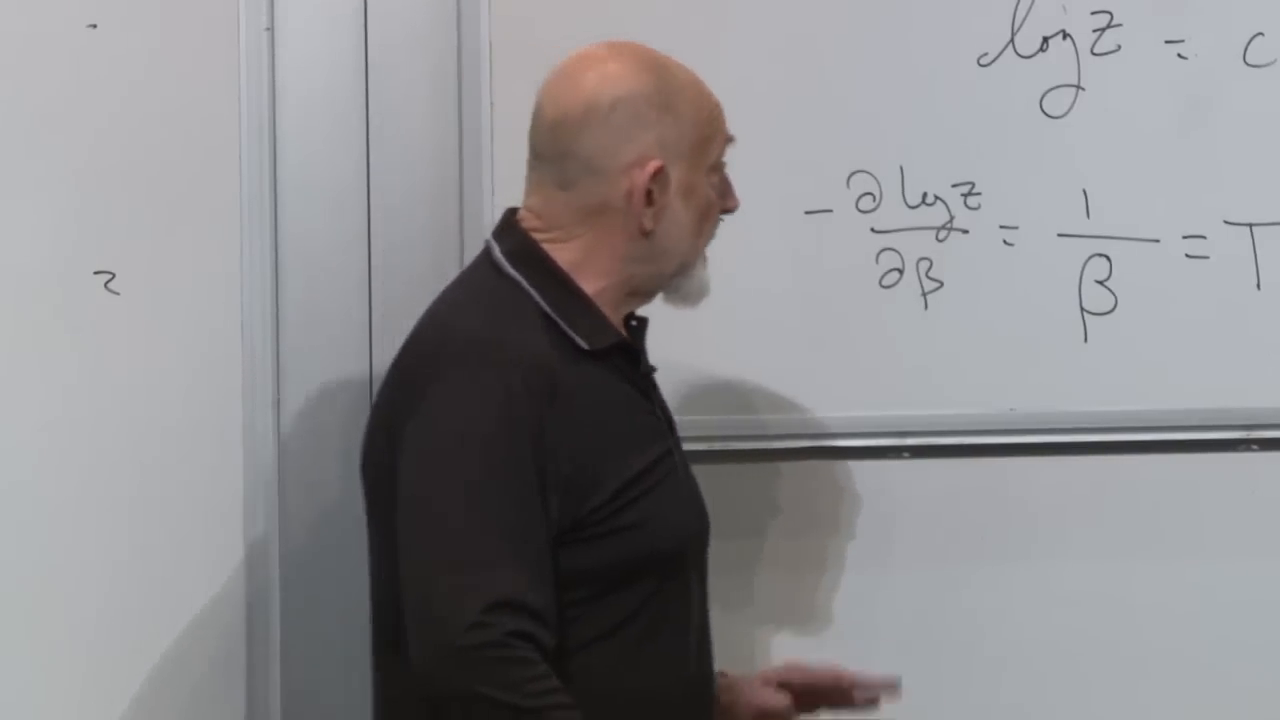
\includegraphics[width=0.90\textwidth]{lecture_07_figure_02.png}
\caption{Die Abschätzung der Molekülgeschwindigkeit, die Druckableitung und das eingesetzte ideale Gasgesetz nebeneinander.}
\lectureframe{00:08:55}
\end{figure}

Eine wichtige Präzisierung ist nötig. Eine Schallwelle kleiner Amplitude komprimiert und entspannt das Gas gewöhnlich schneller, als Wärme zwischen benachbarten Elementen fließen kann. Die lokale Bewegung ist daher näherungsweise adiabatisch, nicht isotherm:
\begin{equation}
 c_s^2=
 \left(\frac{\partial P}{\partial\rho_m}\right)_S.
 \label{eq:sm7-sound-adiabatic}
\end{equation}
Für ein ideales Gas mit dem Adiabatenexponenten \(\gamma\) gilt:
\begin{equation}
 P\rho_m^{-\gamma}=\text{constant},
 \qquad
 c_s^2=\gamma\frac{P}{\rho_m}
       =\gamma\frac{k_B T}{m}.
 \label{eq:sm7-sound-ideal-adiabatic}
\end{equation}
Für Luft bei Raumtemperatur ist \(\gamma\simeq 7/5\). Die Rechnung bei konstanter Temperatur liefert also eine brauchbare erste Abschätzung, während die adiabatische Ableitung die physikalisch angemessene Präzisierung darstellt.

Mit den groben Werten
\begin{equation}
\begin{aligned}
 k_B&\simeq1.3\times10^{-23}\ {\rm J\,K^{-1}},
 &T&\simeq300\ {\rm K},\\
 m_{\rm air}&\simeq4\times10^{-26}\ {\rm kg}.&&
\end{aligned}
 \label{eq:sm7-air-data}
\end{equation}
ergibt die Abschätzung anhand der Molekülgeschwindigkeit etwa \(500\ {\rm m\,s^{-1}}\). Die Temperatur muss hier als absolute Temperatur in Kelvin angegeben werden, nicht auf einer Skala mit einem willkürlichen Nullpunkt wie Fahrenheit. Die vertraute Schallgeschwindigkeit liegt in der Größenordnung von \(300\ {\rm m\,s^{-1}}\), und die adiabatische Formel für das ideale Gas ergibt bei Raumtemperatur etwa \(340\ {\rm m\,s^{-1}}\). Die grobe Rechnung hat somit die richtige physikalische Größenordnung getroffen.

\begin{figure}[t]
\centering
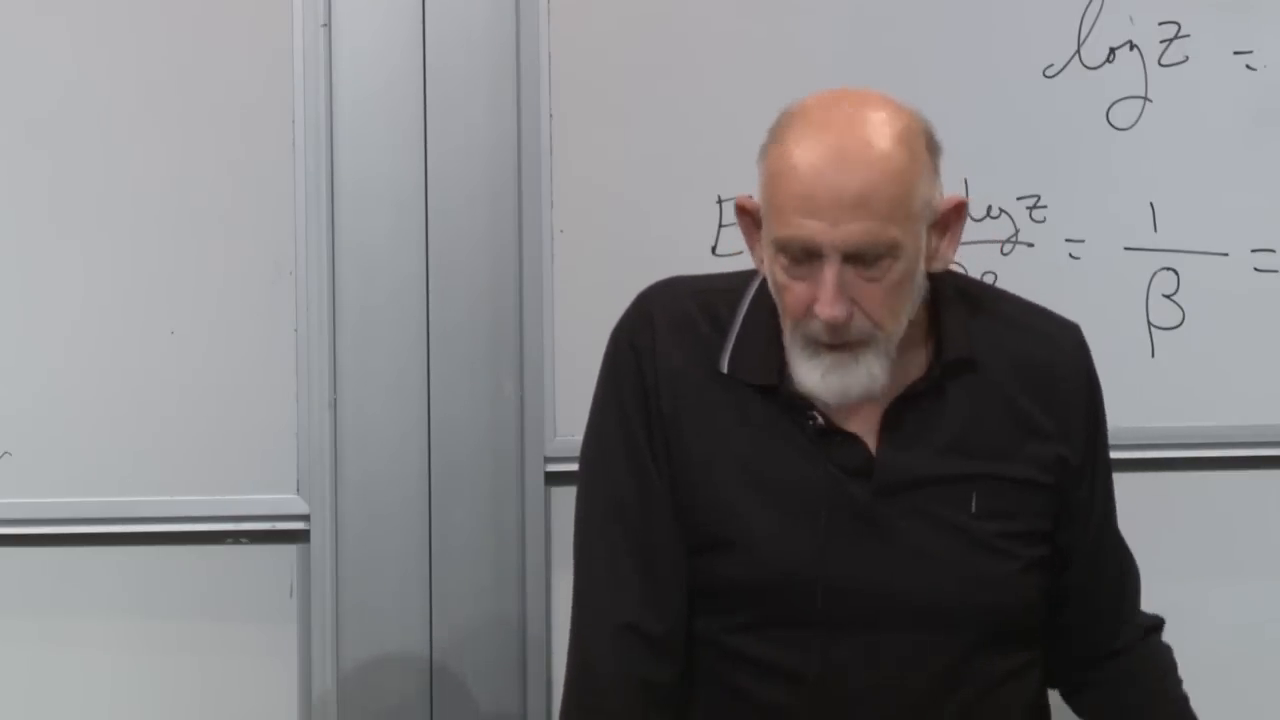
\includegraphics[width=0.90\textwidth]{lecture_07_figure_03.png}
\caption{Abschätzung für Luft bei Raumtemperatur mit der Boltzmann-Konstanten, einer effektiven Molekülmasse von ungefähr \(30\) Protonenmassen und \(T\simeq300\ {\rm K}\).}
\lectureframe{00:10:55}
\end{figure}

Lange bevor eine mikroskopische Erklärung verfügbar war, ließ sich die Schallgeschwindigkeit aus Messungen des Drucks als Funktion der Dichte bestimmen. Die statistische Herleitung liefert die bemerkenswerte Deutung, dass die resultierende makroskopische Geschwindigkeit durch die thermische Geschwindigkeit einzelner Moleküle festgelegt ist.

\begin{classroomqa}
\audiencequestion{Müssen Neutronen zur Molekülmasse hinzugerechnet werden, und zählt die Zahl \(14\) für Stickstoff nur Protonen?}
\lecturerresponse{Das angegebene Atomgewicht berücksichtigt bereits Protonen und Neutronen. Molekularer Stickstoff besteht aus zwei Atomen mit einem Atomgewicht von ungefähr \(14\); seine Masse beträgt also etwa \(28\) Protonenmassen. Für diese Abschätzung reicht es, \(28\) auf \(30\) zu runden.
\lecturetimestamp{00:10:58--00:11:16}}
\end{classroomqa}

\begin{classroomqa}
\audiencequestion{Der Faktor \(3\) stammt von den drei Translationsrichtungen, während sich der Schall in einer Richtung ausbreitet. Müsste der Faktor \(3\) deshalb wegfallen?}
\lecturerresponse{Das ist ein berechtigter Hinweis: Die dreidimensionale quadratische Mittelgeschwindigkeit der Moleküle darf nicht mit einer eindimensionalen Ausbreitungsgeschwindigkeit gleichgesetzt werden. Das einleitende Argument lieferte lediglich eine Größenordnung. Eine fundierte Antwort ergibt sich aus der Druckableitung zusammen mit der für die Welle passenden thermodynamischen Bedingung.
\lecturetimestamp{00:11:12--00:12:00}}
\end{classroomqa}

\begin{classroomqa}
\audiencequestion{Setzte die Ableitung voraus, dass die Temperatur während der Welle konstant bleibt?}
\lecturerresponse{Das Einsetzen des idealen Gasgesetzes in der gezeigten Rechnung tat dies. Für eine sehr kleine Störung ist eine Temperaturkonstanz eine plausible vorläufige Annahme. Die übliche Präzisierung lautet, dass gewöhnlicher Schall näherungsweise adiabatisch ist; dadurch wird die isotherme Ableitung durch \(\left(\partial P/\partial\rho_m\right)_S\) ersetzt.
\lecturetimestamp{00:12:59--00:14:01}}
\end{classroomqa}

\begin{classroomqa}
\audiencequestion{Wenn sowohl die Druck- als auch die Dichteänderungen klein sind, müsste dann nicht auch ihre Ableitung klein sein?}
\lecturerresponse{Nein. Eine Ableitung ist im infinitesimalen Grenzfall das Verhältnis zweier kleiner Änderungen. Sowohl \(\delta P\) als auch \(\delta\rho\) können klein sein, während \(\delta P/\delta\rho\) endlich bleibt und die Wellengeschwindigkeit festlegt.
\lecturetimestamp{00:14:03--00:14:23}}
\end{classroomqa}

\begin{classroomqa}
\audiencequestion{Müsste die Schallgeschwindigkeit steigen, wenn das Gas komprimiert wird, so wie sie beim Übergang vom Gas zur Flüssigkeit oder zum Festkörper steigt?}
\lecturerresponse{Ja. Die Ableitung wird am betrachteten Zustand ausgewertet, und \(P(\rho,T)\) muss nicht linear sein. Werden die Moleküle eng zusammengedrückt, wird die Zustandsgleichung nichtideal, und \(\partial P/\partial\rho\) kann erheblich anwachsen.
\lecturetimestamp{00:14:25--00:15:13}}
\end{classroomqa}

\begin{classroomqa}
\audiencequestion{Kann der Wert \(500\ {\rm m\,s^{-1}}\) bei jedem Druck verwendet werden?}
\lecturerresponse{Nein. Er gilt im Niederdichtebereich, in dem die ideale Gasgleichung eine gute Näherung ist. Sobald in \(P(\rho,T)\) höhere Dichtepotenzen auftreten, hängen die Ableitung und damit die Schallgeschwindigkeit von Druck und Dichte ab.
\lecturetimestamp{00:15:14--00:16:29}}
\end{classroomqa}

\begin{classroomqa}
\audiencequestion{Versagt auch das ursprüngliche Bild, nach dem sich der Schall ungefähr mit der Molekülgeschwindigkeit ausbreitet, wenn die Dichte zunimmt?}
\lecturerresponse{Wahrscheinlich. Dieses Bild ist auf ein verdünntes Gas zugeschnitten. Bei hoher Dichte gewinnen kollektive Wechselwirkungen zunehmend an Bedeutung. Genau deshalb ist die Ableitung der Zustandsgleichung die allgemeinere Beschreibung.
\lecturetimestamp{00:16:32--00:16:53}}
\end{classroomqa}

\begin{classroomqa}
\audiencequestion{Warum wurde die Masse eines Stickstoffmoleküls mit ungefähr \(30\) Protonenmassen angegeben und nicht mit \(28\)?}
\lecturerresponse{Es genügt die für die Abschätzung erforderliche numerische Genauigkeit; deshalb wurde \(28\) auf \(30\) gerundet. Teilt man die ursprüngliche Abschätzung von \(500\ {\rm m\,s^{-1}}\) durch \(\sqrt{3}\simeq1.7\), erhält man ebenfalls ungefähr \(300\ {\rm m\,s^{-1}}\). Die Korrektur lässt sich jedoch fundiert mit der adiabatischen Ableitung berechnen.
\lecturetimestamp{00:16:54--00:17:27}}
\end{classroomqa}

\section{Ein klassischer Oszillator in einem Wärmebad}

Nun ersetzen wir das frei bewegliche Molekül durch einen harmonischen Oszillator und behandeln alles Übrige als Wärmebad. Eine Masse an einer Feder ist das naheliegende Bild, doch das Modell ist viel allgemeiner. Eine elektromagnetische Hohlraummode schwingt; Atome in einem Kristall schwingen; fast jedes stabile System führt bei kleiner Auslenkung aus dem Gleichgewicht näherungsweise eine harmonische Bewegung aus.

Mit \(x\) als Auslenkung aus der Gleichgewichtslage, dem Impuls \(p\), der Masse \(m\) und der Federkonstanten \(\kappa\) lautet der Hamiltonoperator:
\begin{equation}
 H(x,p)=\frac{p^2}{2m}+\frac{\kappa x^2}{2},
 \qquad
 \omega=\sqrt{\frac{\kappa}{m}}.
 \label{eq:sm7-classical-hamiltonian}
\end{equation}
Das Wärmebad legt \(T\) fest, und von hier an verwenden wir wieder \(k_B=1\), sodass \(\beta=1/T\) gilt. Ein Oszillator, der mit einem Raum im Gleichgewicht ist, hat eine Temperatur nahe \(300\ {\rm K}\); in flüssigem Helium beträgt sie nur einige Kelvin. Eine gedachte Feder im Zentrum der Sonne würde nicht als Feder bestehen bleiben, doch das Beispiel verdeutlicht die Rolle der Umgebung. Der Boltzmann-Faktor zerfällt in ein Produkt:
\begin{equation}
 e^{-\beta H}
 =e^{-\beta p^2/(2m)}
  e^{-\beta\kappa x^2/2}.
 \label{eq:sm7-factorized-weight}
\end{equation}

\begin{figure}[t]
\centering
\includegraphics[width=0.90\textwidth]{lecture_07_figure_04.png}
\caption{Ein Feder-Masse-Oszillator und sein Hamiltonoperator als Summe aus kinetischer und potenzieller Energie.}
\lectureframe{00:20:55}
\end{figure}

Anders als beim freien Gas liefert das Ortsintegral nicht einfach das Volumen des Behälters. Das rücktreibende Potenzial gewichtet jede Auslenkung:
\begin{equation}
 Z_{\rm cl}
 =\frac{1}{h}\int_{-\infty}^{\infty}dp
             \int_{-\infty}^{\infty}dx\,
 e^{-\beta p^2/(2m)}
 e^{-\beta\kappa x^2/2}.
 \label{eq:sm7-classical-z}
\end{equation}
Der Faktor \(1/h\) macht die klassische Zustandssumme in einer Dimension dimensionslos. In der Rechnung an der Tafel wird er weggelassen, weil er unabhängig von \(\beta\) ist und die mittlere Energie nicht beeinflussen kann.

\begin{figure}[t]
\centering
\includegraphics[width=0.90\textwidth]{lecture_07_figure_05.png}
\caption{Die klassische Zustandssumme des Oszillators, zerlegt in die Gaußintegrale über Impuls und Auslenkung.}
\lectureframe{00:22:55}
\end{figure}

Für das Impulsintegral setzen wir
\begin{equation}
 q=\sqrt{\frac{\beta}{2m}}\,p,
 \qquad
 dp=\sqrt{\frac{2m}{\beta}}\,dq.
 \label{eq:sm7-p-gaussian-substitution}
\end{equation}
Für das Ortsintegral setzen wir
\begin{equation}
 y=\sqrt{\frac{\beta\kappa}{2}}\,x,
 \qquad
 dx=\sqrt{\frac{2}{\beta\kappa}}\,dy.
 \label{eq:sm7-x-gaussian-substitution}
\end{equation}
Da \(\int_{-\infty}^{\infty}e^{-u^2}\,du=\sqrt{\pi}\), lautet das unnormierte Phasenraumintegral aus der Rechnung an der Tafel:
\begin{equation}
 \int dp\,dx\,e^{-\beta H}
 =\frac{2\pi}{\beta}\sqrt{\frac{m}{\kappa}}
 =\frac{2\pi}{\beta\omega}.
 \label{eq:sm7-classical-z-unnormalized}
\end{equation}
Mit wieder eingesetzter Phasenraumzelle gilt:
\begin{equation}
 Z_{\rm cl}=\frac{2\pi}{h\beta\omega}
           =\frac{1}{\beta\hbar\omega}.
 \label{eq:sm7-classical-z-normalized}
\end{equation}

Für die Energie kommt es nur auf die Abhängigkeit von \(\beta\) an:
\begin{equation}
 \begin{aligned}
 \log Z_{\rm cl}&=\text{constant}-\log\beta,\\
 \expect{H}
 &=-\frac{\partial\log Z_{\rm cl}}{\partial\beta}\\
 &=\frac{1}{\beta}=T.
 \end{aligned}
 \label{eq:sm7-classical-energy}
\end{equation}

\begin{figure}[t]
\centering
\includegraphics[width=0.90\textwidth]{lecture_07_figure_06.png}
\caption{Die vollständige klassische Rechnung auf der rechten Tafel: Gaußfaktorzerlegung, \(Z\propto(\beta\omega)^{-1}\) und \(\expect{H}=1/\beta=T\).}
\lectureframe{00:30:15}
\end{figure}

Es gibt keinen Faktor \(3\), denn dies ist ein räumlicher Oszillator. Auch bleibt kein Faktor \(1/2\) übrig, denn es gibt zwei unabhängige quadratische Terme. Jeder Gaußterm liefert \(T/2\):
\begin{equation}
 \expect{K}=\frac{T}{2},
 \qquad
 \expect{U}=\frac{T}{2},
 \qquad
 \expect{H}=T.
 \label{eq:sm7-equipartition-oscillator}
\end{equation}
Dies ist die Gleichverteilung in ihrer nützlichsten Form: Jeder unabhängige quadratische Term im klassischen Hamiltonoperator trägt \(T/2\) bei.

Die Antwort ist unabhängig von \(m\) und \(\kappa\). Die Bewegung selbst hängt jedoch von diesen Parametern ab:
\begin{equation}
 \expect{p^2}=mT,
 \qquad
 \expect{x^2}=\frac{T}{\kappa},
 \qquad
 \expect{\dot{x}^2}=\frac{T}{m}.
 \label{eq:sm7-classical-fluctuations}
\end{equation}
Eine größere Masse bewegt sich also langsamer, und eine steifere Feder hat eine kleinere Amplitude, obwohl die mittlere Energie \(T\) bleibt. Beunruhigend wird das, wenn \(\kappa\) fantastisch groß wird. Eine Feder, die so steif ist, dass sie sich nicht bewegen kann, sollte wie eine starre Zwangsbedingung wirken; dennoch weist die klassische Gleichverteilung ihr weiterhin die Energie \(T\) zu.

\begin{classroomqa}
\audiencequestion{Wenn \(\kappa\to\infty\), geht die Zustandssumme gegen null. Wie kann ihr Logarithmus dann noch verwendet werden?}
\lecturerresponse{Wir halten \(\kappa\) endlich, aber beliebig groß. Sein Beitrag zu \(\log Z\) ist additiv und unabhängig von \(\beta\), sodass die \(\beta\)-Ableitung weiterhin \(T\) ergibt. Das Unbehagen im Grenzfall ist berechtigt: Die klassische Rechnung ist in sich konsistent, lässt aber eine Eigenschaft der Natur außer Acht, die bei sehr steifen Oszillatoren nötig ist.
\lecturetimestamp{00:34:01--00:34:54}}
\end{classroomqa}

\begin{classroomqa}
\audiencequestion{Für die Zustandssumme des idealen Gases war ein \(N!\) erforderlich. Müsste es hier einen entsprechenden Fakultätsfaktor geben?}
\lecturerresponse{Nein. Wir betrachten einen bestimmten Oszillator, keine Permutationen von \(N\) identischen Teilchen. Bei vielen unabhängigen, unterscheidbaren Moden multiplizieren sich die Zustandssummen. Ein Faktor zur Berücksichtigung der Ununterscheidbarkeit gehört zu einem anderen Zählproblem.
\lecturetimestamp{00:35:03--00:35:40}}
\end{classroomqa}

\section{Warum die klassische Gleichverteilung zur Krise führte}

Reale Moleküle sind keine strukturlosen Punkte. Ein zweiatomiges Molekül enthält eine schwingungsfähige Bindung und damit einen inneren Oszillator. Eine naive klassische Zählung würde dieser Mode selbst bei gewöhnlichen Temperaturen zusätzliche Wärmeenergie zuweisen. In einer bewusst schematischen Rechnung erhöht die Aktivierung eines Schwingungsoszillators die Energie von \(3T/2\) in Richtung \(5T/2\). Für eine genaue Wärmekapazitätsrechnung müssen auch Rotationsfreiheitsgrade berücksichtigt und Energie und ihre Temperaturableitung unterschieden werden. Der entscheidende experimentelle Befund ist einfacher: Steife innere Moden trugen bei niedrigen Temperaturen nicht wie von der klassischen Gleichverteilung gefordert bei.

Man könnte leugnen, dass das Molekül eine innere Struktur hat, was absurd wäre, oder erkennen, dass der klassischen Mechanik eine Zutat fehlt. Diese Zutat ist die Quantenmechanik. Wir brauchen nur wenig davon: nämlich die Tatsache, dass ein harmonischer Oszillator äquidistante Energieniveaus hat.

\section{Der Quantenoszillator}

Zunächst verschieben wir den Energieursprung und schreiben das Anregungsspektrum als
\begin{equation}
 E_n^{\rm exc}=n\hbar\omega,
 \qquad n=0,1,2,\ldots.
 \label{eq:sm7-shifted-spectrum}
\end{equation}
Die Zustandssumme ist nun eine echte Summe statt eines Phasenraumintegrals:
\begin{align}
 Z_{\rm exc}
 &=\sum_{n=0}^{\infty}e^{-\beta n\hbar\omega} \notag\\
 &=1+x+x^2+\cdots
  =\frac{1}{1-x},
 \qquad x=e^{-\beta\hbar\omega}, \notag\\
 &=\frac{1}{1-e^{-\beta\hbar\omega}}.
 \label{eq:sm7-quantum-z}
\end{align}

\begin{figure}[t]
\centering
\includegraphics[width=0.90\textwidth]{lecture_07_figure_07.png}
\caption{Äquidistante Niveaus und Auswertung der geometrischen Reihe für die Zustandssumme des Quantenoszillators.}
\lectureframe{00:42:05}
\end{figure}

Durch Ableiten erhalten wir die mittlere Anregungsenergie:
\begin{align}
 E_{\rm exc}
 &=-\frac{\partial\log Z_{\rm exc}}{\partial\beta}
  =-\frac{1}{Z_{\rm exc}}
    \frac{\partial Z_{\rm exc}}{\partial\beta}
 \notag\\
 &=\hbar\omega\,
   \frac{e^{-\beta\hbar\omega}}
        {1-e^{-\beta\hbar\omega}}
  =\frac{\hbar\omega}{e^{\beta\hbar\omega}-1}.
 \label{eq:sm7-quantum-energy}
\end{align}

\begin{figure}[t]
\centering
\includegraphics[width=0.90\textwidth]{lecture_07_figure_08.png}
\caption{Die thermische Anregungsenergie, ermittelt aus der Ableitung der quantenmechanischen Zustandssumme nach \(\beta\).}
\lectureframe{00:46:05}
\end{figure}

\subsection{Hohe Temperaturen}

Wenn \(\beta\hbar\omega\ll1\), gilt:
\begin{equation}
 e^{-\beta\hbar\omega}
 =1-\beta\hbar\omega
  +O\!\left((\beta\hbar\omega)^2\right).
 \label{eq:sm7-high-t-expansion}
\end{equation}
Der Zähler von \eqref{eq:sm7-quantum-energy} nähert sich \(\hbar\omega\), während der Nenner in führender Ordnung \(\beta\hbar\omega\) ist. Daher gilt:
\begin{equation}
 E_{\rm exc}\simeq\frac{1}{\beta}=T.
 \label{eq:sm7-high-t-energy}
\end{equation}
Bei vielen Niveaudifferenzen innerhalb der thermischen Energie ergibt sich aus dem quantenmechanischen Ergebnis wieder die klassische Gleichverteilung.

\subsection{Niedrige Temperaturen}

Wenn \(\beta\hbar\omega\gg1\), ist die Exponentialfunktion sehr klein:
\begin{equation}
 E_{\rm exc}
 \simeq\hbar\omega e^{-\beta\hbar\omega}.
 \label{eq:sm7-low-t-energy}
\end{equation}
Die thermische Anregung des Oszillators ist exponentiell unterdrückt. In der verschobenen Konvention ist sie fast null; die physikalische Nullpunktsenergie wird weiter unten wieder eingesetzt.

\begin{figure}[t]
\centering
\includegraphics[width=0.90\textwidth]{lecture_07_figure_09.png}
\caption{Entwicklung bei niedriger Temperatur: Die erste thermische Anregung ist durch \(e^{-\beta\hbar\omega}\) unterdrückt.}
\lectureframe{00:51:55}
\end{figure}

Der Übergang findet statt, wenn
\begin{equation}
 \beta\hbar\omega\sim1,
 \qquad\text{or equivalently}\qquad
 T\sim\hbar\omega.
 \label{eq:sm7-crossover}
\end{equation}
Diese Bedingung hat eine direkte Bedeutung. Nach der klassischen Gleichverteilung hätte der Oszillator die Energie \(T\). Quanteneffekte lassen sich nicht mehr vernachlässigen, wenn diese Energieskala unter eine Niveaudifferenz sinkt. Somit gilt:
\begin{equation}
\begin{aligned}
 \hbar\omega\gg T&:\quad \text{frozen and quantum},\\
 \hbar\omega\ll T&:\quad \text{active and classical}.
\end{aligned}
 \label{eq:sm7-regimes}
\end{equation}
Eine steifere Feder hat ein größeres \(\omega=\sqrt{\kappa/m}\) und benötigt daher eine höhere Temperatur, bevor sie sich klassisch verhält.

\section{Mit steigender Temperatur werden Freiheitsgrade sichtbar}

Bei niedriger Temperatur kann ein zweiatomiges Molekül thermisch einem Punktteilchen ähneln, weil seine steife Bindungsschwingung eingefroren ist. Wenn \(T\) \(\hbar\omega\) durchläuft, wird die Schwingungsmode aktiviert. Rotationsmoden können sich schon bei einer niedrigeren Temperaturskala aktivieren; noch höhere Temperaturen machen weitere innere Bewegungen sichtbar und ionisieren schließlich das Atom. Beim Erwärmen wird nicht einfach mehr Energie in eine feste Liste von Moden eingebracht. Es werden Freiheitsgrade sichtbar, die bei niedrigeren Temperaturen unsichtbar waren.

Ein gedachtes verschachteltes Molekül verdeutlicht den Punkt. Zwei Atome sind durch eine steife Feder verbunden; eines der scheinbaren Atome ist selbst ein Paar, das durch eine noch steifere Feder verbunden ist. Bei niedriger Temperatur \(T\) erscheinen beide Strukturen punktförmig. Bei der ersten Schwelle tritt die äußere Schwingung hervor, bei der zweiten wird die innere Struktur sichtbar. Die Komplexität des Systems erschließt sich eine Energieskala nach der anderen.

\begin{classroomqa}
\audiencequestion{Wenn ein Oszillator bereits im klassischen Bereich ist, wird die Feder dann durch weiteres Erwärmen steifer oder ändert sich ihre Frequenz?}
\lecturerresponse{Nein. Federkonstante und Frequenz bleiben unverändert. Eine höhere Temperatur führt zu größeren typischen Impulsen und Amplituden und damit zu größerer Energie. Die Steifigkeit bestimmt die Temperatur, bei der das klassische Gesetz einsetzt, nicht eine temperaturabhängige Versteifung der Feder.
\lecturetimestamp{01:03:17--01:05:11}}
\end{classroomqa}

\subsection{Kristalle und Einsteins spezifische Wärme}

Ein Kristall enthält sehr viele Schwingungsmoden. Die klassische Gleichverteilung weist jedem aktiven Oszillator eine Energie in der Größenordnung von \(T\) zu und überschätzt daher die Wärmekapazität bei niedrigen Temperaturen. Einsteins 1907-Modell behandelte Kristallschwingungen quantenmechanisch und erklärte, warum sie unterdrückt sind, bis die thermische Energie ihre Niveaudifferenz erreicht. Genauere Festkörpermodelle berücksichtigen eine Verteilung der Modenfrequenzen; das Prinzip des Ausfrierens ist jedoch bereits in Einsteins Rechnung enthalten.

\begin{classroomqa}
\audiencequestion{War dies die Arbeit, für die Einstein den Nobelpreis erhielt, und entstand sie erst, nachdem sich die Quantenmechanik etabliert hatte?}
\lecturerresponse{Nein. Die Nobelpreisbegründung bezog sich auf den photoelektrischen Effekt. Das Modell der spezifischen Wärme wurde 1907 veröffentlicht, lange bevor die Grundlagen der Quantenmechanik vollständig verstanden waren. Einstein griff entscheidende Quantenideen auf und entwickelte sie weiter, obwohl er später Aspekten der ausgereiften Theorie widersprach.
\lecturetimestamp{00:58:38--01:03:16}}
\end{classroomqa}

\begin{classroomqa}
\audiencequestion{Die klassische statistische Mechanik ersetzte eine Summe über diskrete Zustände durch ein scheinbar gleichförmiges Integral über Ort und Impuls. Was rechtfertigt diese Zustandszählung?}
\lecturerresponse{Die letztliche Rechtfertigung ergibt sich aus der Quantenmechanik. Im Hochtemperaturgrenzfall,
\[
 Z_{\rm exc}\simeq\frac{1}{\beta\hbar\omega},
\]
was genau mit dem dimensionslosen klassischen Ergebnis \eqref{eq:sm7-classical-z-normalized} übereinstimmt. Wenn die Abstände zwischen den Energieniveaus nicht aufgelöst werden, gehen die quantenmechanischen Zellen im Phasenraum in das klassische Phasenraummaß über.
\lecturetimestamp{00:59:38--01:03:06}}
\end{classroomqa}

\subsection{Eine Saite enthält unendlich viele Oszillatoren}

Eine Violin- oder Gitarrensaite lässt sich in Normalmoden zerlegen: die Grundschwingung, höhere Harmonische und immer kürzere Wellenlängen. Mathematisch gibt es unendlich viele Oszillatormoden. Würde die klassische Gleichverteilung jeder davon die Energie \(T\) zuweisen, hätte die Saite im thermischen Gleichgewicht unendliche Energie. Die Quantenmechanik verhindert diese Katastrophe. Die Moden mit den kürzesten Wellenlängen haben die höchsten Frequenzen und bleiben bei jeder endlichen Temperatur eingefroren; mit zunehmendem \(T\) werden nach und nach mehr Moden aktiviert. Dieselbe Überlegung wird später der Schwarzkörperstrahlung zugrunde liegen.

\begin{figure}[t]
\centering
\includegraphics[width=0.90\textwidth]{lecture_07_figure_10.png}
\caption{Mehrere überlagerte Normalmoden einer Saite veranschaulichen, warum eine kontinuierliche Saite eine unendliche Menge harmonischer Oszillatoren darstellt.}
\lectureframe{01:09:30}
\end{figure}

\begin{classroomqa}
\audiencequestion{Lässt sich der Übergang von der Quanten- zur klassischen Beschreibung direkt beobachten, und kann Erwärmung das Tieftemperaturverhalten umkehren?}
\lecturerresponse{Ja. Die Temperaturabhängigkeit der spezifischen Wärme eines Kristalls macht das Ausfrieren und die anschließende Aktivierung von Schwingungsmoden klar messbar.
\lecturetimestamp{01:09:11--01:10:13}}
\end{classroomqa}

\begin{classroomqa}
\audiencequestion{Wiederholt man bei vielen Oszillatoren für jede Mode die Zustandssumme eines einzelnen Oszillators?}
\lecturerresponse{Für unabhängige Moden gilt
\[
\begin{aligned}
 Z_{\rm tot}&=\prod_j Z_j,&
 \log Z_{\rm tot}&=\sum_j\log Z_j,\\
 E_{\rm tot}&=\sum_j E_j.&&
\end{aligned}
\]
Moden mit \(\hbar\omega_j\gg T\) leisten einen exponentiell kleinen Beitrag zur Wärme; Moden unterhalb dieser Schwelle tragen merklich bei.
\lecturetimestamp{01:10:14--01:11:00}}
\end{classroomqa}

\begin{classroomqa}
\audiencequestion{Was ist aus der Nullpunktsenergie des Oszillators \(\hbar\omega/2\) geworden?}
\lecturerresponse{Die physikalischen Energieniveaus lauten
\[
 E_n=\left(n+\frac12\right)\hbar\omega.
\]
Folglich gilt
\[
 \begin{aligned}
 Z_{\rm phys}
 &=e^{-\beta\hbar\omega/2}Z_{\rm exc},\\
 E_{\rm phys}
 &=\frac{\hbar\omega}{2}
  +\frac{\hbar\omega}{e^{\beta\hbar\omega}-1}.
 \end{aligned}
\]
Der gemeinsame Energieversatz verändert weder die Besetzungswahrscheinlichkeiten der Niveaus noch die Entropie, die Wärmekapazität oder die thermische Anregungsenergie, verschiebt aber die absolute mittlere Energie um \(\hbar\omega/2\). Der Vorfaktor in \(Z\) hängt von \(\beta\) ab und darf daher nicht weggelassen werden, wenn die absolute Energie gesucht ist.
\lecturetimestamp{01:11:08--01:11:37}}
\end{classroomqa}

\section{Der zweite Hauptsatz als Rätsel der Reversibilität}

Nun können wir auf das angekündigte Problem zurückkommen. Der zweite Hauptsatz besagt, dass gewöhnliche makroskopische Entwicklung irreversibel ist und die Entropie tendenziell zunimmt. Die mikroskopische Hamiltonsche Entwicklung ist reversibel. Wie kann eine reversible Abbildung exakter Zustände ein irreversibles Gesetz für makroskopische Zustände hervorbringen?

Wir stellen das System durch einen Punkt in einem hochdimensionalen Phasenraum dar:
\[
 \Gamma=(q_1,\ldots,q_N,p_1,\ldots,p_N).
\]
Unser Wissen entspricht gewöhnlich keinem exakten Punkt. Nehmen wir an, es sei durch eine gleichförmige Wahrscheinlichkeitsdichte auf einem kompakten Gebiet \(A\) mit Volumen \(\Omega_A\) beschrieben:
\begin{equation}
 f(\Gamma)=
 \begin{cases}
  1/\Omega_A,&\Gamma\in A,\\
  0,&\Gamma\notin A.
 \end{cases}
 \label{eq:sm7-uniform-blob}
\end{equation}
In Einheiten mit \(k_B=1\) lautet die feinkörnige Gibbs-Entropie:
\begin{equation}
 S_{\rm fine}
 =-\int d\Gamma\,f\log f
 =\log\Omega_A.
 \label{eq:sm7-blob-entropy}
\end{equation}
Ein kleineres Gebiet bedeutet mehr Information und geringere Entropie. Damit ist das Vorzeichen festgelegt: Größere Ungewissheit vergrößert den besetzten Bereich und erhöht \(\log\Omega_A\).

\begin{figure}[t]
\centering
\includegraphics[width=0.90\textwidth]{lecture_07_figure_11.png}
\caption{Ein kompaktes Wahrscheinlichkeitsgebiet in einem schematischen zweidimensionalen Ausschnitt des vollständigen Orts-Impuls-Phasenraums.}
\lectureframe{01:20:20}
\end{figure}

\begin{classroomqa}
\audiencequestion{Ist das System physikalisch darauf beschränkt, innerhalb des eingezeichneten Bereichs zu bleiben, und befindet es sich bereits im Gleichgewicht?}
\lecturerresponse{Nein. Der Bereich beschreibt, was über den Anfangszustand bekannt ist, und ist keine Wand im Phasenraum. Der Anfangszustand muss keiner Gleichgewichtsverteilung entsprechen. Ein Gas, das anfangs in einem Tank in einer Zimmerecke eingeschlossen ist, liefert ein konkretes Beispiel für spezielle Information über einen Nichtgleichgewichtszustand.
\lecturetimestamp{01:14:55--01:15:24}}
\end{classroomqa}

\section{Liouville-Fluss und Zunahme der grobkörnigen Entropie}

Das Theorem von Liouville besagt, dass der Hamiltonsche Fluss das Phasenraumvolumen erhält. Das exakte Gebiet kann sich verschieben, strecken, falten und extrem dünn werden, aber
\begin{equation}
 \Omega_{A(t)}=\Omega_{A(0)},
 \qquad
 S_{\rm fine}(t)=S_{\rm fine}(0).
 \label{eq:sm7-liouville}
\end{equation}
Das diskrete Analogon ist eine reversible Permutation von Zuständen. Weiß man anfangs, dass ein Würfel in einem von zwei Zuständen ist, kann eine bijektive Entwicklung diese beiden Zustände verändern, nicht aber die Anzahl der Möglichkeiten.

Reale Beschreibungen haben eine endliche Auflösung. Die Quantenmechanik liefert eine natürliche Phasenraumzelle; auch ein klassisches Experiment hat eine endliche Messgenauigkeit, selbst wenn man die Quantentheorie nicht heranzieht. Unter Hamiltonschem Fluss kann das Gebiet zu einer langen, dünnen Schlange werden. Sinkt der Abstand zwischen benachbarten Windungen unter die Auflösungsskala, fassen wir jede nicht aufgelöste Umgebung zu einer grobkörnigen Zelle zusammen. Das exakt besetzte Volumen bleibt konstant, doch die Vereinigung der grobkörnigen Zellen wächst:
\begin{equation}
 \Omega_{\rm coarse}(t)\geq\Omega_{A(t)},
 \qquad
 S_{\rm coarse}(t)=\log\Omega_{\rm coarse}(t).
 \label{eq:sm7-coarse-entropy}
\end{equation}

\begin{figure}[t]
\centering
\includegraphics[width=0.90\textwidth]{lecture_07_figure_12.png}
\caption{Ein volumenbewahrendes Filament, betrachtet mit endlichen Auflösungszellen. Das exakte schwarze Filament behält seine Fläche; die roten grobkörnigen Zellen nehmen einen größeren effektiven Bereich ein.}
\lectureframe{01:22:10}
\end{figure}

\begin{classroomqa}
\audiencequestion{Die grob aufgelösten Zellen überlappen. Verletzt das den Satz von Liouville?}
\lecturerresponse{Nein. Die Liouville-Dynamik betrifft die exakte Faser, die eineindeutig bleibt und das Volumen erhält. Die Überlappung entsteht in unserer unscharfen Beschreibung: Wir haben die Information darüber verworfen, in welchem dünnen Strang sich der Zustand befindet.
\lecturetimestamp{01:21:32--01:21:50}}
\end{classroomqa}

Ein nützlicher Vergleich ist Baumwolle. Das Materialvolumen aller Fasern kann nahezu gleich bleiben, während ein auseinandergezupfter Knäuel für einen Beobachter, der die einzelnen Fasern nicht auflösen kann, ein großes scheinbares Volumen einnimmt. Ebenso bildet ein Phasenraumgebiet immer feinere Tentakel aus; diese Tentakel entwickeln wiederum noch feinere Tentakel. Jede festgelegte endliche Auflösung reicht schließlich nicht mehr aus, um ihnen zu folgen.

\begin{classroomqa}
\audiencequestion{Scheint die Entropie klassisch nur zuzunehmen, während die Quantenmechanik diese Zunahme durch eine fundamentale Auflösungsgrenze real macht?}
\lecturerresponse{Für das Grobkörnig-Argument ist keine quantenmechanische Auflösungsgrenze erforderlich. Die Entropie bezieht sich sowohl auf das System als auch auf die makroskopischen Unterscheidungen, die in seiner Beschreibung erhalten bleiben. Bei unendlicher mikroskopischer Information bleibt die feinkörnige Entropie konstant; bei jeder festen endlichen Auflösung werden chaotische Fasern irgendwann unaufgelöst, und die grobkörnige Entropie nimmt zu.
\lecturetimestamp{01:24:04--01:25:20}}
\end{classroomqa}

\section{Chaos, ein endlicher zugänglicher Bereich und die Einstellung des Gleichgewichts}

Bei einem Gas in einem Kasten sind die Positionen beschränkt. Bei fester endlicher Gesamtenergie sind auch die Impulse beschränkt, selbst wenn sich die gesamte Energie vorübergehend in einem Teilchen konzentriert. Unter den üblichen Einschlussbedingungen hat die dynamisch zugängliche Energieschale daher ein endliches Maß.

\begin{figure}[t]
\centering
\includegraphics[width=0.90\textwidth]{lecture_07_figure_13.png}
\caption{Ein beschränkter zugänglicher Phasenraumbereich neben dem Filament und seiner grobkörnigen Darstellung.}
\lectureframe{01:28:10}
\end{figure}

Nahe beieinanderliegende Anfangspunkte in einem chaotischen System durchlaufen eine Zeit lang ähnliche Entwicklungen und entfernen sich dann voneinander. Bei einem Eröffnungsstoß beim Billard überträgt sich eine unmerkliche Änderung der Richtung des Spielballs auf die folgenden Kollisionen; die Unterschiede summieren sich, bis die Endkonfigurationen nichts mehr miteinander zu tun haben. Ein ganzes anfängliches Gebiet wird daher durch den zugänglichen Bereich gedehnt und gefaltet. Bei endlicher Auflösung nähert sich seine Beschreibung einem breiten, nahezu gleichförmigen Gleichgewichtszustand an.

\begin{figure}[t]
\centering
\includegraphics[width=0.90\textwidth]{lecture_07_figure_14.png}
\caption{Ein kompakter spezieller Zustand entwickelte sich im beschränkten zugänglichen Bereich zu einem komplizierten Filament, während sich die grob aufgelösten Zellen über eine viel größere Fläche verteilten.}
\lectureframe{01:33:10}
\end{figure}

Zwei Einschränkungen sind wichtig. Chaos allein beweist nicht, dass jede Trajektorie jede zugängliche Umgebung besucht; diese stärkere Aussage über das Abtasten des Phasenraums setzt eine ergodische oder mischende Eigenschaft voraus. Auch ist nicht jedes physikalische System chaotisch. Ein generisches Vielteilchengas und idealisierte Billards bilden den hier gemeinten Rahmen, in dem Mischen eine sinnvolle physikalische Erwartung ist.

\section{Rekurrenz hebt die Irreversibilität nicht auf}

Angenommen, alle Luftmoleküle befinden sich anfangs in einer Ecke und haben ein speziell vorbereitetes Geschwindigkeitsmuster. Durch Kollisionen verteilen sie sich rasch im Raum, und die grob aufgelöste Beschreibung erreicht das Gleichgewicht. In einem endlichen, maßtreuen Phasenraum besagt der Rekurrenzsatz von Poincaré, dass fast jeder Anfangspunkt beliebig nahe an seinen Ausgangspunkt zurückkehrt. Für eine Toleranz \(\epsilon>0\) ist eine Rekurrenzzeit \(t_R(\epsilon)\) unter den Voraussetzungen des Satzes endlich, auch wenn sie für ein makroskopisches System unvorstellbar groß ist. Eine exakte Rückkehr zu einem unendlich genau festgelegten Punkt ist weder erforderlich noch im Allgemeinen zu erwarten.

\begin{classroomqa}
\audiencequestion{Führt der Stoß auf den Spielball im Billardbeispiel Energie zu und macht er die abgeschlossene Entwicklung damit zunichte?}
\lecturerresponse{Der gewählte Anfangszustand beginnt unmittelbar nach dem Stoß; die dabei übertragene Energie ist also bereits berücksichtigt. Die Rekurrenz betrifft die anschließende isolierte, idealisierte Billarddynamik. Eine Rückkehr in die Nähe des Anfangszustands umfasst eine Konfiguration, in der sich der Spielball innerhalb der gewählten Toleranz dem Kugeldreieck nähert.
\lecturetimestamp{01:35:37--01:35:55}}
\end{classroomqa}

\begin{classroomqa}
\audiencequestion{Wenn das Gas schließlich in die Ecke zurückkehren kann, haben wir dann Information verloren, und ist das System wirklich reversibel?}
\lecturerresponse{Die mikroskopische Dynamik bleibt durchgehend reversibel. Die grob aufgelöste Entropie kann zunehmen, weil wir feine Korrelationen nicht mehr auflösen; dennoch kann eine außerordentlich seltene Fluktuation das System in die Nähe seines speziellen Anfangsmakrozustands zurückführen. Rekurrenz und grob aufgelöste Irreversibilität sind daher miteinander vereinbar.
\lecturetimestamp{01:37:34--01:38:15}}
\end{classroomqa}

Das führt zu Boltzmanns wesentlicher Formulierung. Die Entropie nimmt nicht in jedem logisch möglichen Augenblick zu. Für einen Nichtgleichgewichtsmakrozustand eines großen Systems führen überwältigend mehr der damit vereinbaren mikroskopischen Fortsetzungen zu größeren Makrozuständen als zu noch spezielleren. Die Entropie nimmt \emph{wahrscheinlich} zu. Abwärtsfluktuationen und Rekurrenzen sind möglich, doch ihre Wahrscheinlichkeiten und Zeitskalen machen sie in der gewöhnlichen makroskopischen Erfahrung unsichtbar. Das Irreversibilitätsproblem war eine der großen historischen Auseinandersetzungen der statistischen Mechanik und lastete schwer auf Boltzmann. Dieser historische Zusammenhang sollte nicht zu einer einfachen Kausalaussage über sein Leben gemacht werden.

\section{Was Chaos bedeutet}

Für eine stärker operationale Definition von Chaos nehmen wir an, dass sich zwei Anfangspunkte im Phasenraum um \(\delta\Gamma(0)\) unterscheiden. In einer chaotischen Richtung gilt typischerweise
\begin{equation}
 \lVert\delta\Gamma(t)\rVert
 \sim e^{\lambda t}\lVert\delta\Gamma(0)\rVert,
 \qquad \lambda>0,
 \label{eq:sm7-lyapunov-growth}
\end{equation}
in dem Bereich, in dem die linearisierte Separation aussagekräftig ist. Die Zahl \(\lambda\) ist ein Lyapunov-Exponent. Um Vorhersagen für eine Zeit \(t\) zu treffen, muss die Genauigkeit der Anfangsdaten ungefähr wie \(e^{-\lambda t}\) skaliert sein. Auch die Genauigkeit des dynamischen Gesetzes spielt eine Rolle: Modellfehler werden ebenso verstärkt wie Fehler der Anfangsbedingungen. Das Wetter ist das bekannte Beispiel.

\begin{classroomqa}
\audiencequestion{Gibt es ein Prinzip, dem zufolge \emph{die meisten} Systeme chaotisch sind, oder ist das lediglich eine empirische Feststellung?}
\lecturerresponse{Es gibt unendlich viele chaotische und nichtchaotische Hamiltonfunktionen; außerdem setzt schon das Wort \emph{die meisten} ein Maß auf dem Raum der Hamiltonfunktionen voraus. Komplizierte wechselwirkende Systeme sind oft chaotisch, aber es gibt keinen einfachen allgemeinen Test, mit dem sich jede Hamiltonfunktion durch bloße Inspektion klassifizieren lässt.
\lecturetimestamp{01:39:27--01:40:49}}
\end{classroomqa}

\begin{classroomqa}
\audiencequestion{Was bedeutet \emph{chaotisch} in dieser Diskussion genau?}
\lecturerresponse{Nahe beieinanderliegende Phasentrajektorien entfernen sich schnell genug voneinander, sodass langfristige Vorhersagen eine exponentiell genauere Kenntnis der Anfangsbedingungen erfordern. Im Gegensatz dazu drehen sich benachbarte Phasenraumpunkte beim harmonischen Oszillator gemeinsam und bleiben nahe beieinander. Auch das exakte Zweikörper-Keplerproblem ist nichtchaotisch, während das allgemeine Dreikörperproblem chaotische Bereiche aufweist.
\lecturetimestamp{01:40:50--01:43:45}}
\end{classroomqa}

\begin{classroomqa}
\audiencequestion{Müssen die Bewegungsgesetze ebenso genau bekannt sein wie die Anfangsbedingungen?}
\lecturerresponse{Ja. Beide Fehlerquellen pflanzen sich durch die Dynamik fort, und die chaotische Entwicklung verstärkt beide.
\lecturetimestamp{01:43:46--01:43:55}}
\end{classroomqa}

Das Doppelpendel ist ein anschauliches Beispiel. Ein gewöhnliches Pendel ist integrabel und vorhersagbar. Fügt man ein zweites Pendel hinzu, können Trajektorien, die fast am selben Ort beginnen, schließlich auf unterschiedliche Weise Energie übertragen und in völlig verschiedene Richtungen laufen.

\begin{figure}[t]
\centering
\includegraphics[width=0.90\textwidth]{lecture_07_figure_15.png}
\caption{Das Doppelpendel als konkretes Beispiel für deterministisches Chaos.}
\lectureframe{01:44:40}
\end{figure}

\begin{classroomqa}
\audiencequestion{Warum kann ein mechanisches System chaotisch sein, ein anderes aber nicht?}
\lecturerresponse{Das ist eine Eigenschaft der Hamiltonfunktion und ihrer invarianten Strukturen, keine Folge von Reibung oder experimentellem Rauschen. Sie zu bestimmen kann mathematisch schwierig sein; Komplexität ist ein Hinweis, aber kein Beweis.
\lecturetimestamp{01:44:03--01:45:58}}
\end{classroomqa}

\begin{classroomqa}
\audiencequestion{Ist ein ideales Doppelpendel auch ohne Reibung chaotisch?}
\lecturerresponse{Ja. Dissipation ist nicht erforderlich. Eine exakte deterministische Hamiltonsche Bewegung kann empfindlich von den Anfangsbedingungen abhängen. Unendlich genaue Anfangsdaten würden die Trajektorie auf unbegrenzte Zeit festlegen; bei endlicher Genauigkeit ist der Vorhersagehorizont jedoch endlich.
\lecturetimestamp{01:45:57--01:47:54}}
\end{classroomqa}

\begin{classroomqa}
\audiencequestion{Ist Chaos dasselbe wie das Fehlen einer geschlossenen Lösung?}
\lecturerresponse{Chaotischen Systemen fehlt im Allgemeinen eine global brauchbare geschlossene Darstellung der Trajektorie, aber analytische Lösbarkeit und empfindliche Abhängigkeit sind verschiedene Eigenschaften. Chaos wird dynamisch anhand der Trennung von Trajektorien diagnostiziert, nicht allein anhand unserer Unfähigkeit, eine Formel anzugeben.
\lecturetimestamp{01:48:20--01:49:23}}
\end{classroomqa}

\begin{classroomqa}
\audiencequestion{Worin unterscheidet sich allgegenwärtiges Chaos davon, genau auf dem instabilen Gipfel eines Hügels zu balancieren?}
\lecturerresponse{Der Hügelgipfel ist ein einzelner, außergewöhnlicher instabiler Zustand: Abseits davon müssen sich benachbarte Trajektorien nicht schnell voneinander entfernen. In einem chaotischen Gebiet ist die Instabilität entlang der Bahn typisch, und benachbarte Phasenraumpunkte entfernen sich wiederholt voneinander. Ein positiver Lyapunov-Exponent erfasst dieses anhaltende Wachstum.
\lecturetimestamp{01:49:27--01:50:11}}
\end{classroomqa}

\section{Von der mikroskopischen Bewegung zum statistischen Gesetz}

Die Abschätzung der Schallgeschwindigkeit zeigte, wie die mikroskopische thermische Bewegung eine makroskopische Ausbreitungsskala festlegt; die Fragen machten zugleich deutlich, welche thermodynamische Ableitung angegeben werden muss. Der Oszillator zeigte anschließend die Reichweite und das Versagen der klassischen Gleichverteilung. Die Quantisierung der Energieniveaus friert steife Moden ein, erklärt, warum sich Wärmekapazitäten mit der Temperatur ändern, und verhindert, dass unendlich viele hochfrequente Moden unendlich viel thermische Energie tragen.

Dieselbe Entwicklung von der exakten Mikrophysik zur effektiven makroskopischen Beschreibung löst den scheinbaren Widerspruch auf, der dem zweiten Hauptsatz zugrunde liegt. Die Hamiltonsche Strömung erhält das exakte Phasenraumvolumen und bleibt reversibel. Chaotisches Dehnen erzeugt feinere Korrelationen, als eine makroskopische Beschreibung erfasst; dadurch wächst der grob aufgelöste besetzte Bereich. Rekurrenz garantiert, dass seltene Rückkehrereignisse nicht ausgeschlossen sind; die Wahrscheinlichkeit erklärt, warum sie nicht zur gewöhnlichen Erfahrung gehören. Der zweite Hauptsatz ist keine neue irreversible mikroskopische Kraft. Er beschreibt die überwältigend zuverlässige statistische Entwicklungsrichtung für spezielle makroskopische Anfangsbedingungen in Systemen mit enorm vielen Freiheitsgraden.
\chapter{Wiederkehr, Nichtgleichgewichtsordnung und Ising-Spins}

\lectureoverview{Ein Gas, das aus einer Raumhälfte freigesetzt wird, strömt dem Gleichgewicht entgegen. Die reversible Mechanik besagt jedoch, dass eine hinreichend lange Entwicklung auch Rückkehrzustände zum Ausnahmezustand hervorbringen muss. Wir schätzen die Rückkehrzeit anhand des Phasenraumvolumens ab, trennen die Wiederkehr vom ungeklärten Beginn des Universums mit niedriger Entropie und nutzen das daraus entstehende Rätsel, um Boltzmann-Gehirne, eine kohärente Geschichte und durch einen Energiefluss aufrechterhaltenes Leben zu erörtern. Anschließend wenden wir uns der magnetischen Ordnung zu. Unabhängige Spins mit zwei möglichen Zuständen liefern einen exakt lösbaren Einstieg: Die Kombinatorik bestimmt die Zustandssumme, und die Magnetisierung ist ein hyperbolischer Tangens. Wechselwirkungen zwischen Nachbarn stellen schließlich eine Auf--ab-Symmetrie wieder her und führen zum eindimensionalen Ising-Modell.}

\section{Ein Raum voller Luft, die schließlich zurückkehrt}

Beginnen wir mit der gesamten Luft in der linken Hälfte eines Raums. Diesen Zustand kann man mithilfe einer Trennwand herstellen: Man evakuiert die rechte Hälfte, bringt die Luft links unter und entfernt dann die Wand. Das Gas breitet sich rasch im Raum aus und nähert sich dem thermischen Gleichgewicht. Die Entropie nimmt zu. Nichts Überraschendes ist geschehen.

Nun lassen wir den Raum verschlossen und warten. Eine Serie von einer Million aufeinanderfolgenden Kopfseiten ist beim Münzwurf ein außerordentlich unwahrscheinliches Ergebnis. Bei einem unbegrenzt oft wiederholten Experiment treten jedoch irgendwann außerordentlich unwahrscheinliche Ergebnisse auf. Für das Gas gilt dieselbe Logik. Zu einem weit in der Zukunft liegenden Zeitpunkt werden sich wieder alle Moleküle in der linken Hälfte oder in einem vergleichbar besonderen Bereich befinden. Eine solche Rückkehr heißt Poincaré-Wiederkehr.

Der genaue Satz ist etwas vorsichtiger formuliert als dieses Bild. Für ein Gebiet endlichen Maßes im Phasenraum, dessen Dynamik das Phasenraumvolumen erhält, kehrt fast jeder Anfangspunkt beliebig nahe an seinen Ausgangspunkt zurück. Eine makroskopische Aussage wie \emph{alle Moleküle befinden sich in der linken Hälfte} ist einfacher: Sie verlangt nur, dass die Bahn erneut in einen endlichen grob aufgelösten Bereich eintritt, nicht, dass jede Molekülkoordinate exakt ihren Ausgangswert annimmt. Die praktische Frage lautet: Wie lange dauert das?

\subsection{Ein hochdimensionaler Phasenraumpunkt}

Für \(N\) klassische Teilchen hat der Phasenraum \(6N\) Koordinaten:
\begin{equation}
 \Gamma=(\bm x_1,\ldots,\bm x_N;\bm p_1,\ldots,\bm p_N).
 \label{eq:sm8-phase-point}
\end{equation}
Die Positionen sind durch den Raum begrenzt. Bei fester Gesamtenergie sind auch die Impulse beschränkt, denn ein Teilchen kann keinen beliebig großen Impuls haben, ohne zugleich beliebig viel Energie zu tragen. Unter den Voraussetzungen des Wiederkehrarguments hat die zulässige Energieschale daher endliches Maß.

Der Phasenraumpunkt bewegt sich deterministisch, doch die Bewegung eines Vielteilchengases ist chaotisch. Benachbarte Bahnen entfernen sich rasch voneinander, wie bei einer Folge von Billardkugelstößen. Nach der Grobkörnigkeit scheint eine lange Bahn den zugänglichen Bereich zu durchstreifen.

\begin{figure}[t]
\centering
\includegraphics[width=0.90\textwidth]{lecture_08_figure_02.png}
\caption{Schematischer Phasenraumbereich mit einer komplizierten Bahn, die ihn durchstreift. Die Zeichnung ist absichtlich niedrigdimensional; das reale Gas befindet sich in einem Raum mit \(6N\) Dimensionen.}
\lectureframe{00:06:41}
\end{figure}

Die niedrigdimensionale Skizze verleitet uns sofort zu einem Fehler. Würde der besondere Zustand die Hälfte des gezeichneten Rechtecks einnehmen, könnte man sagen, dass das Gas die Hälfte seiner Zeit dort verbringen sollte. Doch die Bedingung \emph{jedes Molekül liegt in der linken Hälfte} schränkt jede Positionskoordinate ein, nicht nur eine Koordinate des Phasenraumpunkts.

Betrachten wir nur zwei Teilchen, die sich eindimensional bewegen, mit den Koordinaten \(x_1\) und \(x_2\). Ihr Konfigurationsraum ist ein Quadrat. Die Bedingung \(x_1<L/2\) wählt die Hälfte des Quadrats aus; die Bedingungen \(x_1<L/2\) und \(x_2<L/2\) wählen ein Viertel aus:
\begin{equation}
 P_2=\frac{1}{2}\frac{1}{2}=\frac{1}{4}.
 \label{eq:sm8-two-particle-quarter}
\end{equation}

\begin{figure}[t]
\centering
\includegraphics[width=0.90\textwidth]{lecture_08_figure_07.png}
\caption{Bei zwei eindimensionalen Teilchen stellt das kleinere Quadrat die Konfigurationen dar, in denen beide Koordinaten in der gewählten Raumhälfte liegen.}
\lectureframe{00:07:08}
\end{figure}

Bei drei Teilchen ergibt sich \(1/2^3\), und bei \(N\) Teilchen ergibt sich
\begin{equation}
 P_{\mathrm{half}}(N)
 =\left(\frac{1}{2}\right)^N.
 \label{eq:sm8-half-probability}
\end{equation}
Auf den Exponenten kommt es entscheidend an. Ein Faktor von einem Halb ist gewöhnlich; ein halb hoch einer makroskopischen Teilchenzahl liegt jenseits der gewöhnlichen Vorstellungskraft.

\begin{classroomqa}
\audiencequestion{Müsste das Ergebnis \(1/3^N\) lauten, da sich die Moleküle auch in anderen Raumrichtungen bewegen?}
\lecturerresponse{Das hängt von der Bedingung ab, die man vorgibt. Geht es nur darum, ob sich jedes Teilchen links von der Trennwand befindet, erfüllt jedes Teilchen eine binäre Bedingung, und das Ergebnis lautet \(2^{-N}\). Beschränkt man einen weiteren, unabhängigen Anteil des verfügbaren Ortsraums, kommt ein weiterer Faktor hinzu.
\lecturetimestamp{00:07:47--00:08:05}}
\end{classroomqa}

\section{Phasenraumvolumen, Entropie und Wiederkehrskala}

Dieselbe Abschätzung lässt sich auch ohne Bezug auf Raumhälften formulieren. Der Raum habe das gewöhnliche räumliche Volumen \(V\), und \(v\) sei ein kleinerer Bereich, in dem sich jedes Molekül befinden soll. Lässt man Impulsfaktoren außer Acht, die beiden Makrozuständen gemeinsam sind, lauten die verfügbaren Konfigurationsraumvolumina:
\begin{equation}
 \Omega_{\mathrm{room}}\propto V^N,
 \qquad
 \Omega_{\mathrm{small}}\propto v^N.
 \label{eq:sm8-config-volumes}
\end{equation}
Der langfristige Zeitanteil, der im kleinen Makrozustand verbracht wird, beträgt daher
\begin{equation}
 P(v)
 =\frac{\Omega_{\mathrm{small}}}{\Omega_{\mathrm{room}}}
 =\left(\frac{v}{V}\right)^N.
 \label{eq:sm8-volume-ratio}
\end{equation}

\begin{figure}[t]
\centering
\includegraphics[width=0.90\textwidth]{lecture_08_figure_08.png}
\caption{Das allgemeine Phasenraumvolumenbild an der Tafel: ein kleiner Bereich \(v^N\) innerhalb eines zugänglichen Bereichs \(V^N\), mit dem Verhältnis \(v^N/V^N\).}
\lectureframe{00:10:44}
\end{figure}

In Einheiten mit \(k_B=1\) ist die Entropie der Logarithmus des zugänglichen Phasenraumvolumens. Sind \(S_A=\log\Omega_A\) die Entropie des eingeschränkten Makrozustands und \(S_{\rm eq}=\log\Omega_{\rm eq}\) die des Gleichgewichts, so gilt:
\begin{equation}
 \begin{aligned}
 P(A)
 &=\frac{\Omega_A}{\Omega_{\rm eq}}\\
 &=\exp\!\left(S_A-S_{\rm eq}\right)\\
 &=e^{-\Delta S},\\
 \Delta S&=S_{\rm eq}-S_A.
 \end{aligned}
 \label{eq:sm8-entropy-probability}
\end{equation}
Für den Zustand mit der Luft in einer Raumhälfte ist \(\Delta S=N\log 2\), und \eqref{eq:sm8-entropy-probability} vereinfacht sich exakt zu \(2^{-N}\).
Die Kurzschreibweise \(P\sim e^{-S_{\rm eq}}\) ist nur dann angemessen, wenn die Entropie des besonderen Bereichs als feste Referenz behandelt wird; der physikalisch aussagekräftige Exponent ist das Entropiedefizit \(\Delta S\).

\begin{classroomqa}
\audiencequestion{Ist das das Volumen des Konfigurationsraums und nicht des gesamten Phasenraums?}
\lecturerresponse{Für diesen Vergleich: ja. Wir geben eine Positionsbedingung vor und lassen dabei die Impulsverteilung bei derselben Temperatur unverändert, sodass sich der gemeinsame Faktor im Impulsraum herauskürzt. Eine allgemeine Aussage zur Wiederkehr bezieht sich auf den Phasenraum; diese spezielle Wahrscheinlichkeit lässt sich aus dem Verhältnis der Konfigurationsraumvolumina berechnen.
\lecturetimestamp{00:11:21--00:11:40}}
\end{classroomqa}

Nehmen wir an, das System verliere sein Gedächtnis an seine genaue Position nach einer mikroskopischen Korrelations- oder Mischungszeit \(\tau_{\rm mix}\). Ein seltener Bereich mit Wahrscheinlichkeit \(P(A)\) wird dann auf der Zeitskala
\begin{equation}
 \tau_{\rm rec}
 \sim \frac{\tau_{\rm mix}}{P(A)}
 \sim \tau_{\rm mix}e^{\Delta S}.
 \label{eq:sm8-recurrence-time-general}
\end{equation}
angetroffen. Für die Bedingung mit der halben Raumgröße gilt:
\begin{equation}
 \tau_{\rm rec}\sim\tau_{\rm mix}2^N.
 \label{eq:sm8-recurrence-time-half}
\end{equation}
In der Vorlesung wird bewusst eine grobe Abschätzung mit einer raumtypischen Größe verwendet:
\(N\sim10^{30}\). Das ergibt die einprägsame Zeitskala
\(\tau_{\rm rec}/\tau_{\rm mix}\sim2^{10^{30}}\). Bei gewöhnlicher atmosphärischer Dichte hat ein Raum eher \(10^{27}\) Moleküle. Ersetzt man aber \(10^{30}\) durch \(10^{27}\), ändert das nichts an der Schlussfolgerung: Die Wiederkehrzeit ist weiterhin unvorstellbar viel größer als das Alter des Universums.

\begin{classroomqa}
\audiencequestion{In welchen Einheiten wird die Wiederkehrzeit gemessen? Könnte ein Wechsel von Sekunden zu Stunden oder zu einer extrem kleinen Zeiteinheit die Schlussfolgerung verändern?}
\lecturerresponse{Der Vorfaktor mit der Dimension einer Zeit ist \(\tau_{\rm mix}\); die riesige Zahl ist das dimensionslose Verhältnis \(\tau_{\rm rec}/\tau_{\rm mix}\). Ein Wechsel von Sekunden zu Stunden bedeutet eine Division durch einen gewöhnlichen Umrechnungsfaktor, der gegenüber \(2^{10^{30}}\) vernachlässigbar ist. Wie lange ein einzelner Aufenthalt in der Ecke dauert, hängt auch von den Molekülgeschwindigkeiten ab. Die Abschätzung betrifft die Seltenheit, mit der ein solcher Aufenthalt beginnt. Es gibt auch einen quantenmechanischen Wiederkehrsatz, doch er wird hier nicht benötigt.
\lecturetimestamp{00:17:24--00:19:18}}
\end{classroomqa}

\begin{classroomqa}
\audiencequestion{Was ist der Zweck einer Berechnung für eine Zeit, auf die kein Experiment jemals warten kann?}
\lecturerresponse{Es geht um eine begriffliche Einsicht. Die Berechnung zeigt, in welchem Sinn ein abgeschlossenes mechanisches System reversibel bleibt. Es verbringt fast seine gesamte Zeit nahe dem Gleichgewicht, zeigt aber auf hinreichend langen Zeitskalen auch Fluktuationen zu niedrigerer Entropie. Der zweite Hauptsatz ist daher eine überwältigend wahrscheinliche Aussage über besondere Anfangsdaten und kein mikroskopisches Gesetz, das eine Bewegungsumkehr verbietet.
\lecturetimestamp{00:15:12--00:16:35}}
\end{classroomqa}

\section{Reversibilität und der besondere Anfang}

Wir beginnen bewusst im kleinen Bereich mit der halben Raumgröße. Fast jede benachbarte Bahn verlässt ihn sofort, denn das Phasenraumvolumen außerhalb ist um ein Vielfaches größer als das innerhalb. Das Gas breitet sich rasch aus und wartet danach sehr lange, bevor es zurückkehrt. Diese Asymmetrie zwischen rascher Relaxation und langem Warten widerspricht der reversiblen Mechanik nicht.

Die Zeitumkehr des raschen Entweichens ist nicht die gesamte Wartezeit. Sie ist der kurze, fantastisch gut koordinierte Vorgang, in dem sich gleichgewichtsähnliche Molekülgeschwindigkeiten zufällig so anordnen, dass das Gas \emph{mit einem Schwung} in eine Raumhälfte strömt. Kehrt man am Ende des gewöhnlichen Entweichens jeden Impuls um, durchläuft das Gas den Entweichvorgang rückwärts. Die lange Wartezeit ist die Zeit, die vergehen muss, bis dieses besondere einlaufende Geschwindigkeitsmuster spontan auftritt.

\begin{classroomqa}
\audiencequestion{Bedeutet die Zeitsymmetrie, dass die langsame Wiederkehr in die Ecke genauso lange dauert wie das ursprüngliche Entweichen aus ihr?}
\lecturerresponse{Nein. Vergleichen Sie das Entweichen mit seiner exakten Zeitumkehr. Beide sind rasch. Ungeheuer lange dauert es, im Gleichgewicht auf die genaue einlaufende Fluktuation zu warten, die den umgekehrten Strömungsvorgang auslöst. Betrachtet man einen enorm langen Zeitraum, treten Abweichungen vom Gleichgewicht in beiden Zeitrichtungen mit lokal symmetrischen Verläufen auf.
\lecturetimestamp{00:20:46--00:21:58}}
\end{classroomqa}

Das Wiederkehrargument erklärt folglich nur einen Teil des Zeitpfeils. Es erklärt, warum die Entropie gewöhnlich zunimmt, \emph{wenn} das System in einem Bereich niedriger Entropie begonnen hat. Es erklärt nicht, warum die Anfangsbedingung besonders war. In der Kosmologie wird diese fehlende Voraussetzung zur zentralen Frage: Warum begann das beobachtbare Universum in einem so außergewöhnlich kleinen Bereich seines gravitativen Phasenraums?

\begin{classroomqa}
\audiencequestion{Gilt die Wiederkehr auch für die Kosmologie? Könnte das Universum, nachdem es sich ausgedehnt hat, bei genügend langem Warten wiederkehren?}
\lecturerresponse{Diese Frage lässt sich nicht umgehen, doch die Antwort hängt von der globalen Kosmologie ab. Für ein tatsächlich abgeschlossenes System mit einem endlichen Gleichgewichtszustandsraum liegt eine Wiederkehr nahe. Eine expandierende Raumzeit, Gravitation, Horizonte und ein unendlicher oder nichtstationärer Zustandsraum können die Voraussetzungen verändern. Die hier wichtige, engere Erkenntnis lautet: Ein Bild der Wiederkehr ins Gleichgewicht reicht für sich genommen nicht als statistische Erklärung des strukturierten Universums, das wir beobachten.
\lecturetimestamp{00:19:59--00:20:45}}
\end{classroomqa}

\begin{classroomqa}
\audiencequestion{Hängt die Wiederkehr davon ab, dass das Gas zu Beginn in einem kleinen Bereich präpariert wird? Wenn der Raum im Gleichgewicht beginnt, sammelt sich die Luft dann irgendwann trotzdem in einer Ecke?}
\lecturerresponse{Ja. Bei der Wiederkehr geht es um die Langzeitdynamik des abgeschlossenen Systems. Daher unterliegen auch gleichgewichtsähnliche Anfangszustände seltenen Fluktuationen zu niedriger Entropie. Den Zustand mit der Luft in einer Raumhälfte vorzubereiten ist aus einem anderen Grund wichtig: So können wir von einem bekannten besonderen Anfangszustand ausgehen und fragen, warum die Entropie unmittelbar danach zunimmt.
\lecturetimestamp{00:22:04--00:22:20}}
\end{classroomqa}

\section{Warum eine zufällige Fluktuation zu wenig vorhersagt}

Man könnte versuchen, aus der Wiederkehr eine Kosmologie zu entwickeln: Vielleicht verbrachte das Universum fast eine ganze Ewigkeit im Gleichgewicht, und unsere heutige Welt ist eine seltene Fluktuation. Dieser Vorschlag besteht eine scharfe statistische Prüfung nicht. Nehmen wir die Existenz eines Beobachters als Bedingung und fragen wir, was dieser Beobachter sonst noch erwarten sollte.

Eine Fluktuation, die groß genug ist, um einen Planeten hervorzubringen, ist außerordentlich selten. Eine Fluktuation, die zwei Planeten hervorbringt, erfordert ein größeres Entropiedefizit und ist noch seltener. Eine Fluktuation, die Sterne, Galaxien, einen kosmischen Mikrowellenhintergrund und untereinander konsistente Aufzeichnungen einer langen Vergangenheit hervorbringt, ist um einen enormen zusätzlichen Exponentialfaktor seltener. Eine Theorie der Gleichgewichtsfluktuationen sagt daher die kleinste Fluktuation voraus, die für eine Beobachtung ausreicht, und nicht die reichhaltige kohärente Welt, die tatsächlich beobachtet wird. In ihrer extremsten Form heißt der minimale Beobachter Boltzmann-Gehirn.

Die Logik beruht auf bedingten Wahrscheinlichkeiten. Sei \(A\) das Ereignis, dass eine Fluktuation in der Größenordnung eines Beobachters auftritt, und \(B\) eine davon unabhängige zweite Struktur. Haben beide eine geringe Wahrscheinlichkeit \(p\), so gilt:
\begin{equation}
 P(B\mid A)=p,
 \qquad
 P(A\cap B)=p^2.
 \label{eq:sm8-conditional-fluctuations}
\end{equation}
Zu erfahren, dass die erste Fluktuation aufgetreten ist, macht die zweite nicht wahrscheinlich. Die Analogie zur Lotterie trifft genau auf dieser Ebene zu: Ein früherer Gewinner hat bei der nächsten unabhängigen Ziehung keine besseren Chancen. Der Beobachter kann also seine eigene Anwesenheit als Bedingung setzen, sollte aber weiterhin erstaunt sein, wenn er eine unabhängig strukturierte Umgebung vorfindet.

\begin{classroomqa}
\audiencequestion{Ist die Wahrscheinlichkeit für einen weiteren Planeten oder einen weiteren Boltzmann-Beobachter wirklich geringer, wenn es bereits einen Planeten oder Boltzmann-Beobachter gibt?}
\lecturerresponse{Die bedingte Wahrscheinlichkeit für eine zweite, unabhängige seltene Fluktuation ist dieselbe geringe Ein-Ereignis-Wahrscheinlichkeit, nicht deren Quadrat. Die gemeinsame Wahrscheinlichkeit für beide beträgt das Quadrat davon. Genau deshalb sollte der erste Beobachter außerhalb seiner selbst weiterhin thermische Unordnung erwarten. Einen Ehepartner, einen weiteren Planeten und einen geordneten Himmel vorzufinden, ist ein Hinweis gegen die Annahme, dass der Beobachter als isolierte Gleichgewichtsfluktuation entstanden ist.
\lecturetimestamp{00:26:12--00:30:27}}
\end{classroomqa}

\subsection{Kohärente Aufzeichnungen einer Vergangenheit}

Dasselbe Argument gilt für die Geschichte. Zwei übereinstimmende Lehrbücher, astronomische Aufzeichnungen, die zu derselben Expansionsgeschichte passen, geologische Schichten, Erinnerungen und Laborbücher schränken einander ein. Ein einzelnes zufälliges Lehrbuch könnte irgendeine Geschichte enthalten. Ein ganzes Netz von Aufzeichnungen, die dieselbe Vergangenheit schildern, nimmt einen viel kleineren Phasenraumbereich ein.

Das Beispiel aus der Vorlesung greift die bekannte Erzählung auf, George Washington habe einen Kirschbaum gefällt. Ob diese Erzählung wahr ist, spielt keine Rolle. Entscheidend ist: In einer Welt, die im gegenwärtigen Augenblick durch eine Fluktuation entstanden wäre, gäbe es keinen dynamischen Grund dafür, dass die Aussage in einem Buch mit einem anderen Zeugnis übereinstimmt. Kohärente Korrelationen sprechen für eine gemeinsame Geschichte und nicht bloß für einen einmaligen Zufall im gegenwärtigen Augenblick.

\begin{classroomqa}
\audiencequestion{Was bedeutet hier \emph{historische Kohärenz}?}
\lecturerresponse{Es bedeutet, dass viele gegenwärtige Aufzeichnungen zueinander passen und sich als Folgen einer gemeinsamen Vergangenheit verstehen lassen. Eine Fluktuation könnte Aufzeichnungen und Erinnerungen hervorbringen, doch ein untereinander konsistentes Netz zu erzeugen erfordert eine viel größere Fluktuation als die Hervorbringung eines einzelnen minimalen Beobachters. Die Wiederkehrtheorie sagt daher voraus, dass es den meisten beobachterähnlichen Fluktuationen an der Kohärenz fehlt, die wir tatsächlich vorfinden.
\lecturetimestamp{00:30:30--00:31:12}}
\end{classroomqa}

\begin{classroomqa}
\audiencequestion{Könnte das Universum dennoch ein abgeschlossenes System sein, dessen Zeit bis zum Gleichgewicht und bis zur Wiederkehr lediglich extrem lang ist?}
\lecturerresponse{Diese Möglichkeit beseitigt das statistische Problem nicht. Im Verlauf einer unbegrenzt langen Geschichte gäbe es viele beobachterähnliche Fluktuationen, und die überwältigende Mehrheit davon wären minimale Fluktuationen ohne kohärente Umgebungsgeschichte. Ein aus diesem Ensemble ausgewählter Beobachter sollte unsere Beobachtungen nicht erwarten. Kosmologinnen und Kosmologen nehmen das Boltzmann-Gehirn-Problem daher als Prüfung kosmologischer Maße und Spätzeitmodelle ernst, nicht als Behauptung, die Wiederkehr sei bereits beobachtet worden.
\lecturetimestamp{00:31:13--00:32:42}}
\end{classroomqa}

\section{Leben als Struktur, die durch einen Fluss aufrechterhalten wird}

Leben scheint die entgegengesetzte Schwierigkeit aufzuwerfen. Organismen erhalten ihre komplexe Organisation lange Zeit aufrecht; sie sehen nicht wie kurzlebige zufällige Fluktuationen aus. Die Auflösung besteht darin, dass der zweite Hauptsatz für ein vollständiges abgeschlossenes System gilt. Ein Teilsystem kann seine Entropie verringern oder aufrechterhalten, sofern in seiner Umgebung eine größere Entropiezunahme stattfindet:
\begin{equation}
 \dot S_{\rm total}
 =\dot S_{\rm subsystem}+\dot S_{\rm environment}\geq 0.
 \label{eq:sm8-open-system-second-law}
\end{equation}

Die Erde befindet sich nicht im thermischen Gleichgewicht. Auf menschlichen Zeitskalen ist sie annähernd stationär, doch stationär bedeutet nicht statisch. Energie durchströmt sie. Sonnenlicht trifft ein, wird durch viele Prozesse abgewertet und bei einer niedrigeren effektiven Temperatur wieder abgestrahlt. Dieser Durchsatz kann lokale Ordnung aufrechterhalten, während die Gesamtentropie zunimmt.

Wasser, das durch ein Rohr fließt, liefert ein unmittelbares mechanisches Bild. In der Strömung können beständige Wirbel und Walzen auftreten. Sie sind geordnete Strukturen, werden aber von der Strömung aufrechterhalten. Verschließt man beide Enden und stoppt die Strömung, lässt die Viskosität die Wirbel verschwinden, während sich das Wasser einem wenig aufregenden Gleichgewicht nähert. Das ausströmende Wasser ist wärmer als das einströmende; das größere System hat also den Entropiepreis entrichtet.

\begin{classroomqa}
\audiencequestion{Verringert das Leben die Entropie, und warum kann seine Organisation fortbestehen, anstatt wie eine gewöhnliche Fluktuation aufzutreten und wieder zu verschwinden?}
\lecturerresponse{Leben kann die Entropie lokal aufrechterhalten oder verringern, aber nur, indem es noch mehr Entropie exportiert. Es besteht dank eines stationären Nichtgleichgewichtsflusses fort, vor allem dank des Flusses von Sonnenenergie durch die Erde. Wäre die Erde gegen ein- und ausgehende Strahlung abgeschlossen, würde sie sich schließlich dem thermischen Gleichgewicht nähern, und die organisierte Aktivität käme zum Erliegen. Leben ähnelt eher einem Wirbel in einer Strömung als einer Gleichgewichtsfluktuation.
\lecturetimestamp{00:32:43--00:35:42}}
\end{classroomqa}

Damit verlassen wir die \emph{interessanten Dinge} und wenden uns, wie es in der bewusst trockenen Formulierung der Vorlesung heißt, etwas Langweiligem zu: Magneten.

\section{Einen Magneten abkühlen: Domänen und eine gewählte Richtung}

In der statistischen Mechanik wird ein mathematisches Modell oft als Magnet bezeichnet, auch wenn es sich nicht um ein Stück Eisen im wörtlichen Sinn handelt. Die nützliche Gemeinsamkeit besteht darin, dass eine Sammlung lokaler Freiheitsgrade Ordnung ausbilden kann. In einem realen magnetischen Material können diese Freiheitsgrade von atomaren magnetischen Momenten, Elektronenspins, orbitalen Strömen oder effektiven Momenten von Kristalleinheiten herrühren.

Bei hoher Temperatur sorgt thermische Unordnung dafür, dass die lokalen Momente in viele Richtungen zeigen, sodass die resultierende Magnetisierung gering ist oder ganz verschwindet. Haben benachbarte Momente eine niedrigere Energie, wenn sie ausgerichtet sind, können sich beim Abkühlen kleine ausgerichtete Domänen bilden. Bei weiterer Abkühlung gewinnt der energetische Vorteil an Bedeutung, und die korrelierten Domänen wachsen. In einem System, das einen ferromagnetischen Übergang aufweist, wird die Korrelationslänge bei einer endlichen kritischen Temperatur makroskopisch. Die geordnete Phase wählt dann eine Orientierung, obwohl die Energie bei verschwindendem Feld keine Orientierung von vornherein bevorzugt hat.

\begin{classroomqa}
\audiencequestion{Müssten sich mikroskopische Magnete aufgrund der Anziehung zwischen Nord- und Südpol bevorzugt entgegengesetzt ausrichten?}
\lecturerresponse{Die effektive Wechselwirkung hängt vom Material ab. Die gewöhnliche Dipolvorstellung erfasst das mikroskopische Problem nicht vollständig; Austauschwechselwirkung, Kristallstruktur und konkurrierende Wechselwirkungen spielen ebenfalls eine Rolle. Ferromagnetische Materialien sind solche, bei denen die effektive Tendenz bei niedriger Energie eine parallele Ordnung begünstigt; andere Materialien können eine entgegengesetzte Ausrichtung bevorzugen.
\lecturetimestamp{00:39:56--00:40:30}}
\end{classroomqa}

\begin{classroomqa}
\audiencequestion{Muss während des Abkühlens des Materials ein äußeres Magnetfeld vorhanden sein, damit sich die Momente ausrichten?}
\lecturerresponse{Nein. Die Wechselwirkung kann auch ohne Feld Ordnung hervorbringen. In einer exakt symmetrischen Idealisierung sind verschiedene Richtungen energetisch gleichwertig. Welche Richtung sich tatsächlich einstellt, wird daher durch anfängliche Fluktuationen, Randbedingungen oder ein beliebig kleines Streufeld bestimmt. Die Auswahl einer dieser gleichwertigen Richtungen ist spontane Symmetriebrechung; der Beginn makroskopischer Ordnung ist der magnetische Phasenübergang.
\lecturetimestamp{00:40:31--00:42:33}}
\end{classroomqa}

Reale Materialien sind kompliziert, deshalb vereinfachen wir jetzt drastisch. Jedes lokale Moment darf nur nach oben oder nach unten zeigen:
\begin{equation}
 \sigma_i=+1\quad\hbox{or}\quad\sigma_i=-1.
 \label{eq:sm8-ising-spin}
\end{equation}
In diesem Modell gibt es weder Osten noch Westen. Die beiden erlaubten Orientierungen sind eine Modellannahme, so wie Kopf und Zahl die beiden möglichen Ergebnisse eines Münzwurfs sind. Der Wert des Modells liegt nicht in seiner mikroskopischen Realitätsnähe, sondern in seiner mathematischen Klarheit und darin, dass es Ordnungsphänomene darstellen kann, die viele Systeme gemeinsam haben.

\begin{classroomqa}
\audiencequestion{Was sind diese Objekte mit zwei Zuständen physikalisch? Sollte man sie sich als Teilchen vorstellen?}
\lecturerresponse{Man kann sich Atome an den Gitterplätzen eines Kristalls vorstellen, von denen jedes ein effektives magnetisches Moment besitzt, das durch Spin oder mikroskopische Ströme entsteht. Für das Modell zählt jedoch nur die Variable mit zwei möglichen Werten. Die Beschränkung auf oben und unten wird eingeführt, um die statistische Mechanik zu vereinfachen.
\lecturetimestamp{00:44:22--00:45:01}}
\end{classroomqa}

\section{Unabhängige Spins in einem äußeren Feld}

Das erste Modell umfasst \(N\) Spins, die nicht miteinander wechselwirken. Ein äußeres Feld \(H\) liefert die einzige Energieskala, und \(\mu\) gibt die Stärke der Kopplung eines einzelnen Spins an dieses Feld an. Wir behalten die in der Rechnung verwendete Vorzeichenkonvention bei:
\begin{equation}
 \epsilon_i=\mu H\sigma_i.
 \label{eq:sm8-single-spin-energy}
\end{equation}
Für \(H>0\) hat ein nach oben gerichteter Spin \(\sigma_i=+1\) die Energie \(+\mu H\), während ein nach unten gerichteter Spin \(\sigma_i=-1\) die Energie \(-\mu H\) hat. Nach dieser Konvention begünstigt ein positives Feld also nach unten gerichtete Spins. Das ist die Umkehrung einer anderen verbreiteten Bezeichnungskonvention. Für die Physik sind die Bezeichnungen jedoch unerheblich, solange die Vorzeichen durchgehend konsistent verwendet werden.

Sei \(n\) die Zahl der nach oben gerichteten Spins und \(m\) die Zahl der nach unten gerichteten Spins. Dann gilt:
\begin{equation}
 n+m=N,
 \qquad
 E=(n-m)\mu H.
 \label{eq:sm8-counting-energy}
\end{equation}

\begin{figure}[t]
\centering
\includegraphics[width=0.90\textwidth]{lecture_08_figure_03.png}
\caption{Die Konfiguration unabhängiger Spins: \(n\) nach oben gerichtete Spins, \(m\) nach unten gerichtete Spins, \(n+m=N\) und \(E=(n-m)\mu H\).}
\lectureframe{00:49:50}
\end{figure}

\begin{classroomqa}
\audiencequestion{Welche Dimensionen haben \(H\), \(\mu\) und \(E\)? Ist \(H\) eine Zahl oder ein Magnetfeld?}
\lecturerresponse{\(H\) bezeichnet die Stärke des von außen angelegten Feldes und \(\mu\) das magnetische Moment. Ihr Produkt \(\mu H\) hat die Dimension einer Energie. Im abstrakten Modell fasst man sie oft zu einem einzigen Parameter mit Energiedimension zusammen, der üblicherweise ebenfalls mit einem kleinen \(h\) bezeichnet wird. Hier behalten wir beide Faktoren bei, um ihren physikalischen Ursprung zu zeigen, und \(E\) ist die Gesamtenergie.
\lecturetimestamp{00:48:21--00:49:27}}
\end{classroomqa}

\subsection{Konfigurationen zählen}

Bei festem \(n\) und \(m=N-n\) wählen wir aus, welche \(n\) der \(N\) Gitterplätze nach oben zeigen. Die Multiplizität beträgt:
\begin{equation}
 \Omega(n,m)=\binom{N}{n}
 =\frac{N!}{n!\,m!}.
 \label{eq:sm8-spin-multiplicity}
\end{equation}
Alle diese Konfigurationen haben dieselbe Energie:
\eqref{eq:sm8-counting-energy}.

\begin{classroomqa}
\audiencequestion{Können \(n\) und \(m\) beide Summationsindizes sein, obwohl sie nicht unabhängig sind? Und wo geht der kombinatorische Faktor ein?}
\lecturerresponse{Man kann sie als Paar mit der Nebenbedingung \(n+m=N\) schreiben oder über \(n=0,\ldots,N\) summieren und \(m=N-n\) setzen. Das Boltzmann-Gewicht gehört zu jeder einzelnen Konfiguration; fasst man alle Konfigurationen gleicher Energie zusammen, wird dieses Gewicht mit \(N!/(n!\,m!)\) multipliziert.
\lecturetimestamp{00:52:04--00:53:03}}
\end{classroomqa}

Die Zustandssumme lautet daher:
\begin{align}
 Z_N
 &=\sum_{n+m=N}
   \frac{N!}{n!\,m!}
   e^{-\beta\mu H(n-m)}
 \notag\\
 &=\sum_{n=0}^{N}
   \binom{N}{n}
   \left(e^{-\beta\mu H}\right)^n
   \left(e^{+\beta\mu H}\right)^{N-n}.
 \label{eq:sm8-spin-z-sum}
\end{align}
Wir führen ein:
\begin{equation}
 x=e^{-\beta\mu H},
 \qquad
 y=e^{+\beta\mu H}.
 \label{eq:sm8-xy}
\end{equation}
Mit dem binomischen Lehrsatz ist die Rechnung dann abgeschlossen:
\begin{align}
 Z_N
 &=\sum_{n=0}^{N}\binom{N}{n}x^n y^{N-n}
   =(x+y)^N
 \notag\\
 &=\left(e^{-\beta\mu H}+e^{+\beta\mu H}\right)^N
   =\left[2\cosh(\beta\mu H)\right]^N.
 \label{eq:sm8-spin-z-closed}
\end{align}

\begin{figure}[t]
\centering
\includegraphics[width=0.90\textwidth]{lecture_08_figure_04.png}
\caption{Die Summe für die Zustandssumme, die Substitutionen \(x\) und \(y\) sowie die Reduktion mit dem binomischen Lehrsatz auf eine Potenz von \(2\cosh(\beta\mu H)\).}
\lectureframe{00:56:00}
\end{figure}

Es gibt auch eine kürzere Herleitung. Da die Spins unabhängig sind, gilt für einen Spin:
\begin{equation}
 z_1=e^{-\beta\mu H}+e^{+\beta\mu H}
    =2\cosh(\beta\mu H),
 \label{eq:sm8-one-spin-z}
\end{equation}
und \(Z_N=z_1^N\). Die kombinatorische Herleitung lohnt sich dennoch, weil sie ausdrücklich zeigt, wie die Multiplizität mit der Energie konkurriert.

\section{Konfigurationsmagnetisierung und Magnetisierung des Ensembles}

Für eine einzelne Konfiguration definieren wir den dimensionslosen Spinüberschuss pro Gitterplatz als:
\begin{equation}
 M_{\rm conf}=\frac{n-m}{N}.
 \label{eq:sm8-config-magnetization}
\end{equation}
Er reicht von \(+1\) bei lauter nach oben gerichteten Spins bis \(-1\) bei lauter nach unten gerichteten Spins. Die hier verwendete thermodynamische Magnetisierung ist der Boltzmann-Mittelwert dieser Größe:
\begin{equation}
 M=\left\langle M_{\rm conf}\right\rangle
  =\left\langle\frac{n-m}{N}\right\rangle.
 \label{eq:sm8-average-magnetization}
\end{equation}
Der Faktor \(\mu H\) gehört nicht in diese Definition. Während der Rechnung stand er kurz darin und wurde dann wieder entfernt; \(\mu H\) wandelt den Spinüberschuss in Energie um.

Für jede einzelne Konfiguration gilt:
\begin{equation}
 E=N\mu H M_{\rm conf}.
 \label{eq:sm8-energy-config-m}
\end{equation}
Aus der Linearität der Mittelwertbildung folgt unmittelbar:
\begin{equation}
 \langle E\rangle=N\mu H M.
 \label{eq:sm8-energy-average-m}
\end{equation}

\begin{figure}[t]
\centering
\includegraphics[width=0.90\textwidth]{lecture_08_figure_05.png}
\caption{Die Spinreihe, der korrigierte Mittelwert der Magnetisierung und die an der Tafel hervorgehobene Energiebeziehung.}
\lectureframe{01:01:22}
\end{figure}

\begin{classroomqa}
\audiencequestion{Wird die Magnetisierung einer bestimmten Konfiguration zugeordnet, oder sprechen wir von einer mittleren Magnetisierung? Warum gilt dieselbe Beziehung auch für die mittlere Energie?}
\lecturerresponse{Beide Begriffe kommen vor und müssen unterschieden werden. \((n-m)/N\) ist der Wert in einer einzelnen Konfiguration; \(M\) ist der Boltzmann-Mittelwert davon. Da \(E=N\mu H M_{\rm conf}\) in jeder einzelnen Konfiguration gilt, ergibt das Mitteln beider Seiten mit denselben Wahrscheinlichkeiten \(\langle E\rangle=N\mu H M\). Die festen Größen \(N\), \(\mu\) und \(H\) können aus dem Mittelwert herausgezogen werden.
\lecturetimestamp{00:59:54--01:03:40}}
\end{classroomqa}

\begin{classroomqa}
\audiencequestion{Wie kann das Modell alle Spins nach Norden--Süden ausrichten, ohne Aufwärts- gegenüber Abwärtsspinorientierungen zu bevorzugen?}
\lecturerresponse{Das Fehlen von Ost und West ist im Zweizustandsmodell fest eingebaut; es ist eine Einschränkung der erlaubten Freiheitsgrade. Das vorliegende Modell mit äußerem Feld \emph{ist} zwischen Aufwärts- und Abwärtsspinorientierungen verzerrt: Bei unserer Vorzeichenkonvention senkt das Feld die Energie der Abwärtsspins. Folglich besitzt dieses Modell keine Aufwärts--Abwärts-Symmetrie. Das weiter unten eingeführte Ising-Modell ohne äußeres Feld wird diese Symmetrie wiederherstellen.
\lecturetimestamp{01:03:41--01:04:53}}
\end{classroomqa}

\subsection{Energie aus der Zustandssumme}

Die mittlere Energie ergibt sich aus der üblichen Identität
\begin{equation}
 \langle E\rangle
 =-\frac{\partial}{\partial\beta}\log Z_N.
 \label{eq:sm8-energy-identity}
\end{equation}
Mit \eqref{eq:sm8-spin-z-closed} folgt
\begin{align}
 \log Z_N
 &=N\log 2+N\log\!\left[\cosh(\beta\mu H)\right],
 \notag\\
 \langle E\rangle
 &=-N\mu H\,
   \frac{\sinh(\beta\mu H)}{\cosh(\beta\mu H)}
 \notag\\
 &=-N\mu H\tanh(\beta\mu H).
 \label{eq:sm8-average-energy}
\end{align}
Zusammen mit \eqref{eq:sm8-energy-average-m} ergibt sich
\begin{equation}
 \boxed{M=-\tanh(\beta\mu H)}.
 \label{eq:sm8-magnetization-tanh}
\end{equation}

Die Form des Ergebnisses enthält die Physik. Man erinnere sich:
\begin{equation}
 \cosh x=\frac{e^x+e^{-x}}{2},
 \qquad
 \sinh x=\frac{e^x-e^{-x}}{2}.
 \label{eq:sm8-hyperbolic-definitions}
\end{equation}
In der Nähe des Ursprungs gilt \(\tanh x=x+O(x^3)\); für große positive Werte von \(x\) nähert sich der Ausdruck \(1\). Da \(\beta=1/T\), gilt
\begin{equation}
 M\longrightarrow -1
 \quad (T\longrightarrow0),
 \qquad
 M\longrightarrow 0
 \quad (T\longrightarrow\infty).
 \label{eq:sm8-magnetization-limits}
\end{equation}
Bei null Temperatur befindet sich jeder Spin im energieärmeren Abwärtszustand. Bei unendlicher Temperatur sind alle Konfigurationen gleich gewichtet, und der Einfluss des Feldes verschwindet. Eine Umkehr von \(H\) kehrt \(M\) um.

\begin{figure}[t]
\centering
\includegraphics[width=0.90\textwidth]{lecture_08_figure_09.png}
\caption{Die Kurve des hyperbolischen Tangens nähert sich für große Werte von \(\beta\mu H\) einem konstanten Wert und verläuft in der Nähe des Ursprungs linear. Die physikalische Magnetisierung gemäß der Konvention in der Vorlesung ist das Negative der dargestellten Funktion \(\tanh\).}
\lectureframe{01:13:14}
\end{figure}

\begin{classroomqa}
\audiencequestion{Die Magnetisierung ändert sich stetig. Wo liegt die zuvor erwähnte Phasenübergangstemperatur?}
\lecturerresponse{In diesem Modell gibt es keine. Unabhängige Spins in einem von null verschiedenen äußeren Feld sind zu einfach, und \(\log Z_N=N\log[2\cosh(\beta\mu H)]\) ist bei jeder positiven endlichen Temperatur eine glatte Funktion. Ein Phasenübergang erfordert das wechselwirkende, symmetrische Problem, dem wir uns nun zuwenden; das zweidimensionale Ising-Modell ohne äußeres Feld ist das erste Modell dieser Familie mit einem Phasenübergang bei endlicher Temperatur.
\lecturetimestamp{01:14:47--01:15:11}}
\end{classroomqa}

\section{Das Ising-Modell: Energie benachbarter Spinpaare}

Das äußere Feld gab eine Richtung vor, noch bevor die statistische Betrachtung begann. Wir entfernen das Feld und lassen die benachbarten Spins einander ein effektives Feld liefern. Zeigen beide Nachbarn eines Gitterplatzes nach oben, begünstigen sie die Aufwärtsrichtung; zeigen beide nach unten, begünstigen sie die Abwärtsrichtung; zeigt einer in jede Richtung, heben sich ihre Wirkungen im einfachsten Bild auf. Die Energie ist nun den Spinpaaren statt einzelnen Gitterplätzen zugeordnet.

Für zwei benachbarte Spins wählen wir \(J>0\) und schreiben
\begin{equation}
 E_{12}=-J\sigma_1\sigma_2.
 \label{eq:sm8-pair-energy}
\end{equation}
Parallel ausgerichtete Spins haben \(\sigma_1\sigma_2=+1\) und die Energie \(-J\); antiparallel ausgerichtete Spins haben das Produkt \(-1\) und die Energie \(+J\). Das Minuszeichen sorgt also genau dafür, dass die Wechselwirkung ferromagnetisch ist.

\begin{figure}[t]
\centering
\includegraphics[width=0.90\textwidth]{lecture_08_figure_06.png}
\caption{Die lokale ferromagnetische Wechselwirkung \(E_{12}=-J\sigma_1\sigma_2\).}
\lectureframe{01:19:59}
\end{figure}

Für eine offene eindimensionale Kette lautet der Hamiltonoperator
\begin{equation}
 {\cal H}=-J\sum_{i=1}^{N-1}\sigma_i\sigma_{i+1}.
 \label{eq:sm8-ising-chain-open}
\end{equation}
Bei periodischen Randbedingungen setzt man \(\sigma_{N+1}=\sigma_1\) und summiert bis \(N\). Bei beiden Konventionen wird jedes benachbarte Paar genau einmal gezählt; bei einer langen Kette wird der Unterschied an den Rändern vernachlässigbar.

\begin{figure}[t]
\centering
\includegraphics[width=0.90\textwidth]{lecture_08_figure_10.png}
\caption{Der Hamiltonoperator der Kette mit nächsten Nachbarn ergibt sich aus der lokalen Paarenergie.}
\lectureframe{01:20:46}
\end{figure}

Bei unendlicher Temperatur sind alle Spinfolgen gleich wahrscheinlich. Im Mittel ist die Hälfte der Bindungen parallel und die andere Hälfte antiparallel ausgerichtet, also gilt
\begin{equation}
 \left\langle\sigma_i\sigma_{i+1}\right\rangle_{T=\infty}=0,
 \qquad
 \left\langle{\cal H}\right\rangle_{T=\infty}=0.
 \label{eq:sm8-infinite-t-bond}
\end{equation}
Die Energie null entspricht hier keinem Zustand niedriger Energie. Der vollständig ausgerichtete Grundzustand hat pro Bindung die Energie \(-J\); das Ensemble bei unendlicher Temperatur liegt daher energetisch extensiv oberhalb davon.

\begin{classroomqa}
\audiencequestion{Wie kann das mittlere Produkt null sein, wenn jedes einzelne Produkt \(\sigma_i\sigma_{i+1}\) entweder \(+1\) oder \(-1\) ist?}
\lecturerresponse{Ein Mittelwert muss nicht zu den Werten gehören, die eine einzelne Konfiguration annimmt. Bei unendlicher Temperatur treten parallele und antiparallele Bindungen gleich häufig auf, sodass sich ihre Beiträge \(+1\) und \(-1\) aufheben. Dieselbe Unterscheidung beim Mitteln, die für die Magnetisierung wichtig war, gilt auch hier.
\lecturetimestamp{01:21:39--01:22:37}}
\end{classroomqa}

\subsection{Zwei Grundzustände und eine globale Symmetrie}

Bei null Temperatur soll jede Bindung parallel ausgerichtet sein. Daher gibt es zwei Grundzustände:
\begin{equation}
 (+,+,+,\ldots,+)
 \qquad\hbox{and}\qquad
 (-,-,-,\ldots,-).
 \label{eq:sm8-two-ground-states}
\end{equation}
Sie haben exakt dieselbe Energie. Am Hamiltonoperator lässt sich diese Entartung unmittelbar erkennen: Man kehrt alle Spins um,
\begin{equation}
 \sigma_i\longmapsto-\sigma_i
 \qquad\hbox{for all }i,
 \label{eq:sm8-global-flip}
\end{equation}
und jedes Bindungsprodukt bleibt unverändert,
\begin{equation}
 (-\sigma_i)(-\sigma_{i+1})
 =\sigma_i\sigma_{i+1}.
 \label{eq:sm8-global-flip-invariance}
\end{equation}
Das Umklappen eines einzelnen Spins ist keine Symmetrie, weil dadurch das Vorzeichen der benachbarten Bindungsprodukte umgekehrt wird. Das Umklappen aller Spins ist dagegen eine Symmetrie. Es handelt sich um die globale \(\mathbb Z_2\)-Symmetrie des Ising-Modells ohne äußeres Feld.

\begin{figure}[t]
\centering
\includegraphics[width=0.90\textwidth]{lecture_08_figure_11.png}
\caption{Der Hamiltonoperator der Kette neben der globalen Transformation \(\sigma_i\mapsto-\sigma_i\), die jedes Paarprodukt invariant lässt.}
\lectureframe{01:26:31}
\end{figure}

Wir legen bei strikt null Temperatur ein winziges Feld an einen Spin an. Dadurch wird die Entartung der beiden Grundzustände aufgehoben, und die ferromagnetischen Kopplungen übertragen diese Auswahl auf die gesamte Kette. Wird das Feld entfernt, nachdem der Zustand ausgewählt wurde, kann ein großes System seine Ausrichtung sehr lange beibehalten. Dies ist der intuitive Zugang zur spontanen Symmetriebrechung.

Dabei ist eine wesentliche statistische Einschränkung zu beachten. Für ein endliches System bei exakt verschwindendem Feld weist das kanonische Ensemble den beiden Grundzuständen dasselbe Gewicht zu und hat daher eine mittlere Magnetisierung von null. Eine Phase mit gebrochener Symmetrie wird definiert, indem man den thermodynamischen Grenzfall vor dem Entfernen des ausrichtenden Feldes bildet:
\begin{equation}
 M_*=\lim_{H\to0^+}\lim_{N\to\infty}M_N(H).
 \label{eq:sm8-order-of-limits}
\end{equation}
Im eindimensionalen Modell mit nächsten Nachbarn ist dieser Grenzwert nur bei \(T=0\) von null verschieden; jede endliche Temperatur zerstört die Fernordnung in der unendlichen Kette. In zwei Dimensionen bleibt die geordnete Phase unterhalb einer von null verschiedenen kritischen Temperatur bestehen.

\subsection{Eine historische Korrektur}

In der Darstellung im Hörsaal wird diese Geschichte mit einem Scherz auf Kosten Isings erzählt. Die tatsächliche Chronologie ist freundlicher. Wilhelm Lenz schlug das Modell vor, und sein Student Ernst Ising löste den eindimensionalen Fall in seiner Dissertation von 1924, die 1925 veröffentlicht wurde. Ising fand korrekt, dass es in einer Dimension keinen ferromagnetischen Phasenübergang bei endlicher Temperatur gibt, auch wenn die größere Bedeutung höherer Dimensionen damals noch nicht verstanden war. Kramers und Wannier entwickelten die zweidimensionale Dualität und bestimmten 1941 den kritischen Punkt des quadratischen Gitters; Onsager gab 1944 die berühmte exakte Lösung ohne äußeres Feld an.

Die nächste Rechnung liegt nun auf der Hand. Wir müssen die Zustandssumme von \eqref{eq:sm8-ising-chain-open} bestimmen und untersuchen, wie ihre Korrelationen von der Temperatur abhängen. Diese Rechnung wird explizit zeigen, warum die eindimensionale Kette keinen Phasenübergang bei endlicher Temperatur besitzt und warum die Dimension eine Rolle spielt.

\section{Zwischenbilanz}

Das Rekurrenzproblem und das Spinproblem veranschaulichen dieselbe statistische Einsicht auf zwei Arten. Im Gas macht ein Entropiedefizit einen Makrozustand exponentiell unwahrscheinlich:
\begin{equation}
 P(A)=e^{-\Delta S},
 \qquad
 \tau_{\rm rec}\sim\tau_{\rm mix}e^{\Delta S}.
 \label{eq:sm8-summary-recurrence}
\end{equation}
Die reversible Mechanik lässt die Rückkehr zu, während das enorme Verhältnis der Phasenraumvolumina erklärt, warum wir im Alltag nur die Relaxation beobachten. Das verbleibende Problem der Zeitrichtung liegt in der besonderen kosmologischen Anfangsbedingung, nicht in einem Versagen der mikroskopischen Reversibilität.

Für unabhängige Spins in einem Feld gilt
\begin{equation}
 Z_N=\left[2\cosh(\beta\mu H)\right]^N,
 \qquad
 M=-\tanh(\beta\mu H).
 \label{eq:sm8-summary-spins}
\end{equation}
Dieses System ist ausdrücklich verzerrt und ändert sich glatt mit der Temperatur. Die Ising-Wechselwirkung
\begin{equation}
 {\cal H}=-J\sum_i\sigma_i\sigma_{i+1}
 \label{eq:sm8-summary-ising}
\end{equation}
entfernt die äußere Verzerrung, stellt eine globale Aufwärts--Abwärts-Symmetrie wieder her und stellt die eigentliche Frage nach der Ordnung: Kann ein symmetrisches Vielteilchensystem bei einer von null verschiedenen Temperatur einen von zwei geordneten Zuständen auswählen?

\chapter{Ising-Korrelationen, mittleres Feld und spontane Magnetisierung}

\lectureoverview{Eine eindimensionale Ising-Kette lässt sich exakt lösen, indem man die Spins an den Gitterplätzen durch Bindungsvariablen ersetzt. Diese Variablentransformation macht die Zustandssumme zu einem Produkt und zeigt, dass jede Korrelation bei endlicher Temperatur exponentiell abklingt. Höherdimensionale Gitter verhalten sich anders, weil jeder Spin Informationen von vielen Nachbarn erhält. Behandelt man ihren Gesamteinfluss als mittleres Feld, erhält man eine Selbstkonsistenzgleichung, eine kritische Temperatur im mittleren Feld und eine präzise Beschreibung dafür, wie ein beliebig kleines äußeres Feld eine der magnetisierten Phasen auswählt.}

\section{Was Ising tatsächlich herausfand}

Der historische Sachverhalt sollte korrekt dargestellt werden. Ernst Ising löste das eindimensionale Modell, das Wilhelm Lenz ihm vorgegeben hatte, und fand zutreffend keinen Phasenübergang bei endlicher Temperatur. Zu weit ging er mit der Schlussfolgerung, dass dasselbe Ergebnis in jeder Dimension gelten müsse. Das ist nicht der Fall. Bereits das zweidimensionale Modell besitzt eine geordnete Phase bei niedrigen Temperaturen.

Eine exakte Lösung in höherer Dimension wäre für den vorliegenden Zweck zu anspruchsvoll. Eine physikalisch anschauliche Näherung genügt, um den Übergang sichtbar zu machen, wenn jeder Spin viele Nachbarn hat. Bevor wir diese Näherung verwenden, lohnt es sich jedoch, die eindimensionale Kette exakt zu lösen. Der Vergleich zwischen der exakten eindimensionalen Antwort und der Näherung für hohe Dimensionen zeigt, welcher Mechanismus in einer Dimension fehlt.

Ein Phasenübergang bedeutet hier mehr als eine allmähliche Verstärkung einer bereits bestehenden Bevorzugung. Überschreitet die Temperatur einen kritischen Wert, erhält der Gleichgewichtszustand eine neue makroskopische Eigenschaft: Eine von null verschiedene Magnetisierung kann bestehen bleiben, selbst nachdem das äußere Feld entfernt wurde, mit dem die Probe ausgerichtet wurde. Die Rechnung muss daher zwei getrennte Fragen beantworten. Bewahrt ein weit entfernter Spin die Orientierung eines ausgewählten Spins, und kann ein infinitesimales Feld eine beliebig große Probe ordnen?

\section{Ein Spin als wiederverwendbarer Grundbaustein}

Betrachten wir eine Variable mit zwei Zuständen
\begin{equation}
\sigma=\pm1,
\end{equation}und wählen die Energiekonvention
\begin{equation}
E(\sigma)=-J\sigma,
\qquad J>0.
\end{equation}
Der Zustand \(\sigma=+1\) hat dann die niedrigere Energie. Der Parameter \(J\) kann für das Produkt aus magnetischem Moment und angelegtem Feld stehen; in diese Rechnung geht jedoch nur das Produkt ein.

Wir betrachten diesen Spin als kleines Teilsystem im thermischen Gleichgewicht mit allem Übrigen. Seine Zustandssumme lautet
\begin{align}
z
&=\sum_{\sigma=\pm1}e^{-\beta E(\sigma)}
 =\sum_{\sigma=\pm1}e^{\beta J\sigma} \\
&=e^{\beta J}+e^{-\beta J}
 =2\cosh(\beta J).
\end{align}

Dasselbe Ergebnis ließe sich auf eine Gesamtheit von \(N\) unabhängigen Spins übertragen. Die vollständige Zustandssumme wäre einfach \(Z=z^N\), also wäre \(\log Z=N\log z\) und jede extensive thermodynamische Größe das \(N\)-Fache ihres Werts für einen einzelnen Spin. Diese Betrachtung als Teilsystem ersetzt die längere kombinatorische Zählung der Spins, die nach oben oder unten zeigen, enthält aber dieselbe Information.
Die mittlere Energie ergibt sich aus der logarithmischen Ableitung:
\begin{align}
\expect{E}
&=-\frac{\partial}{\partial\beta}\log z \\
&=-J\frac{\sinh(\beta J)}{\cosh(\beta J)}
 =-J\tanh(\beta J).
\end{align}
Da \(E=-J\sigma\) gilt,
\begin{equation}
\expect{\sigma}=\tanh(\beta J).
\end{equation}

\begin{figure}[ht]
\centering
\includegraphics[width=0.80\textwidth]{lecture_09_figure_02.png}
\caption{Energie und Magnetisierung eines einzelnen Spins in der Form des hyperbolischen Tangens.}
\lectureframe{00:10:06}
\end{figure}

Diese eine Formel umfasst beide Temperaturgrenzfälle. Bei niedriger Temperatur gilt \(\beta J\gg1\), und der Spin befindet sich mit sehr hoher Wahrscheinlichkeit im Zustand niedrigerer Energie. Bei hoher Temperatur gilt \(\beta J\ll1\), sodass
\begin{equation}
\expect{\sigma}\simeq \beta J\longrightarrow0.
\end{equation}
Die thermische Bewegung hebt die energetische Bevorzugung auf.

\begin{classroomqa}
\audiencequestion{Müsste die mittlere Energie nicht ein Minuszeichen haben?}
\lecturerresponse{Ja. Die thermodynamische Identität lautet \(\expect{E}=-\partial_\beta\log z\), also ergibt sich \(-J\tanh(\beta J)\). Teilt man anschließend durch den Faktor \(-J\) in \(E=-J\sigma\), erhält man die positive Magnetisierung \(\expect{\sigma}=\tanh(\beta J)\). \lecturetimestamp{00:09:15--00:09:44}}
\end{classroomqa}

\section{Die eindimensionale Kette}

Wir ordnen \(N\) Spins auf einer offenen Kette an und lassen benachbarte Spins miteinander wechselwirken:
\begin{equation}
H=-J\sum_{i=1}^{N-1}\sigma_i\sigma_{i+1},
\qquad \sigma_i=\pm1.
\label{eq:ising-chain}
\end{equation}
Für \(J>0\) trägt ein paralleles Paar \(-J\) bei, ein antiparalleles Paar dagegen \(+J\). Die beiden Grundzustände sind daher
\begin{equation}
(+,+,\ldots,+)
\qquad\text{and}\qquad
(-,-,\ldots,-).
\end{equation}

\begin{figure}[ht]
\centering
\includegraphics[width=0.80\textwidth]{lecture_09_figure_03.png}
\caption{Der Hamiltonoperator der offenen Kette und die zugehörige Boltzmann-Summe.}
\lectureframe{00:19:15}
\end{figure}

Der Wechsel von \(J\) zu \(-J\) begünstigt alternierende Spins. Bei einer offenen Kette oder einer geraden periodischen Kette führt die Umdefinition
\begin{equation}
\widetilde{\sigma}_i=(-1)^i\sigma_i
\end{equation}
das Vorzeichen der antiferromagnetischen Kopplung auf das ferromagnetische zurück. Der Unterschied ist physikalisch, doch die Algebra der Zustandssumme ist in einer Dimension dieselbe. Die bekannte Ausnahme ist eine ungerade periodische Kette, da sie wegen der Frustration nicht alternieren kann.

\begin{classroomqa}
\audiencequestion{Gibt es im Hamiltonoperator der Kette ein äußeres Magnetfeld?}
\lecturerresponse{Noch nicht. Gleichung~\eqref{eq:ising-chain} enthält nur eine Kopplung zwischen nächsten Nachbarn. Später fügen wir ein homogenes äußeres Feld als separaten Term \(-h\sum_i\sigma_i\) hinzu, um gezielt zu prüfen, wie der geordnete Zustand auf eine beliebig kleine Bevorzugung reagiert. \lecturetimestamp{00:18:54--00:19:13}}
\end{classroomqa}

\subsection{Gedächtnis als Korrelationsfunktion}

Nehmen wir an, \(\sigma_i\) sei bekanntermaßen nach oben gerichtet. Beeinflusst diese Information einen Spin im Abstand von \(r\) Bindungen? Das Maß dafür ist
\begin{equation}
C(r)=\expect{\sigma_i\sigma_{i+r}}.
\end{equation}
Nähert sich \(C(r)\) für \(r\to\infty\) einem von null verschiedenen Wert, bewahrt das System eine langreichweitige Erinnerung. Nähert sich die Korrelation null, verschwindet der Einfluss des ersten Spins schließlich.

Das Stille-Post-Spiel liefert die passende Anschauung. Jede Person gibt ein binäres Symbol an die nächste weiter. Ist jede Übermittlung fehlerfrei, bleibt das ursprüngliche Bit unbegrenzt erhalten. Tritt bei jedem Schritt eine noch so kleine Fehlerwahrscheinlichkeit auf, geht die ursprüngliche Nachricht durch die wiederholte Übermittlung schließlich verloren. Die Temperatur null entspricht im Ising-Modell dem Fall fehlerfreier Übertragung. Bei jeder positiven Temperatur sind gelegentliche Abweichungen zwischen Nachbarn möglich.

Zur Veranschaulichung mit Zahlen nehmen wir an, dass eine einzelne Übertragung die Zuverlässigkeit \(0.99\) hat. Zwei fehlerfreie Übertragungen erfolgen mit Wahrscheinlichkeit \(0.99^2=0.9801\), und jeder weitere Schritt liefert einen zusätzlichen Faktor \(0.99\). Schon nach hundert Schritten treten häufig Fehler auf; nach zehntausend Schritten ist das Gedächtnis praktisch ausgelöscht. In der Ising-Kette verwendet man ein vorzeichenbehaftetes Maß der Zuverlässigkeit statt dieser Wahrscheinlichkeit für fehlerfreie Übertragung, doch die multiplikative Abnahme ist dieselbe Idee.

Die Analogie wird exakt, sobald man eine Wahrscheinlichkeit von einer Korrelation unterscheidet. Ist \(p\) die Wahrscheinlichkeit, dass benachbarte Spins übereinstimmen, gilt
\begin{equation}
\expect{\sigma_i\sigma_{i+1}}
=p-(1-p)=2p-1.
\end{equation}
Die Größe, die sich also von Bindung zu Bindung multipliziert, ist die überschüssige Zuverlässigkeit \(2p-1\), nicht \(p\) selbst.

\section{Bindungsvariablen und die exakte Zustandssumme}

Die entscheidende Variablentransformation beschreibt Beziehungen statt einzelner Spins:
\begin{equation}
\mu_i=\sigma_i\sigma_{i+1},
\qquad i=1,\ldots,N-1.
\label{eq:bond-variable}
\end{equation}
Jede Bindungsvariable ist bei übereinstimmenden Spins \(+1\) und bei unterschiedlichen Spins \(-1\). Ist der erste Spin festgelegt, bestimmen die Bindungen alle folgenden Spins:
\begin{align}
\sigma_2&=\sigma_1\mu_1,\\
\sigma_3&=\sigma_1\mu_1\mu_2,\\
\sigma_{r+1}&=\sigma_1\prod_{k=1}^{r}\mu_k.
\end{align}
Es gibt keine Redundanz. Die Daten \((\sigma_1,\mu_1,\ldots,\mu_{N-1})\) sind gleichwertig mit \((\sigma_1,\ldots,\sigma_N)\).

In diesen Variablen lautet die Energie einfach
\begin{equation}
H=-J\sum_{i=1}^{N-1}\mu_i.
\end{equation}
Aus den wechselwirkenden Variablen an den Gitterplätzen sind unabhängige Bindungsvariablen geworden. Summiert man zunächst über die beiden Werte von \(\sigma_1\), erhält man
\begin{align}
Z_N
&=2\sum_{\{\mu_i=\pm1\}}
\exp\left(\beta J\sum_{i=1}^{N-1}\mu_i\right)\\
&=2\prod_{i=1}^{N-1}
\left(\sum_{\mu_i=\pm1}e^{\beta J\mu_i}\right)\\
&=2\left[2\cosh(\beta J)\right]^{N-1}.
\label{eq:chain-partition}
\end{align}
Es gibt \(N-1\) Faktoren, denn eine offene Kette mit \(N\) Gitterplätzen hat \(N-1\) Bindungen.

Der führende Faktor zwei steht für die globale Wahl des ersten Spins. Er trägt nur \(\log2\) zu \(\log Z_N\) bei, während die Bindungen einen Term proportional zu \(N-1\) liefern. Für die exakte Zählung bei endlicher Größe ist der Faktor wichtig, doch für die freie Energiedichte verschwindet sein Beitrag im Grenzfall \(N\to\infty\). Deshalb konnte der Tafeltext ihn als „keine große Sache“ bezeichnen, ohne ihn tatsächlich wegzulassen.

\begin{figure}[ht]
\centering
\includegraphics[width=0.82\textwidth]{lecture_09_figure_04.png}
\caption{Der Hamiltonoperator in Gitterplatzvariablen, umgeschrieben als Summe über unabhängige Bindungen, und die daraus resultierende faktorisierte Zustandssumme.}
\lectureframe{00:35:35}
\end{figure}

\begin{classroomqa}
\audiencequestion{Was geschah mit der Summe im Exponenten, als die endgültige Antwort zu einer Potenz wurde?}
\lecturerresponse{Zunächst wurde daraus ein Produkt, und daraus wiederum eine Potenz:
\[
e^{\beta J\sum_i\mu_i}=\prod_i e^{\beta J\mu_i}.
\]
Die Summe über alle Bindungskonfigurationen zerfällt dann in eine Zweitermsumme für jede Bindung. Da jeder Faktor \(2\cosh(\beta J)\) ist, ergibt das Produkt die Potenz \((N-1)\). Schreibt man den Fall mit drei Spins und zwei Bindungen aus, wird die Faktorisierung ganz explizit. \lecturetimestamp{00:33:25--00:35:36}}
\end{classroomqa}

Dies ist eine einfache duale Beschreibung: Gekoppelte Variablen an den Gitterplätzen werden durch ungekoppelte Variablen auf den Bindungen ersetzt. Der Begriff \emph{Dualität} passt hier, weil dasselbe System zwei Beschreibungen mit sehr unterschiedlich wirkenden Freiheitsgraden besitzt. Bei einer offenen eindimensionalen Kette handelt es sich um eine exakte Variablentransformation.

In der Sprache des Gitters leben die ursprünglichen Variablen auf den Knoten und die neuen auf den Kanten. Die globale Wahl des ersten Spins ist die zusätzliche Angabe, die benötigt wird, um die Knoten aus den Kanten zu rekonstruieren. Dieser Austausch von Gitterplätzen und Bindungen ist ein einfaches Beispiel für ein Muster, das in der statistischen Mechanik höherer Dimensionen wesentlich mächtiger wird.

\subsection{Zuverlässigkeit zwischen nächsten Nachbarn}

Jede Bindung hat dieselbe Verteilung,
\begin{equation}
\begin{aligned}
\Pr(\mu=+1)&=\frac{e^{\beta J}}{2\cosh(\beta J)},\\
\Pr(\mu=-1)&=\frac{e^{-\beta J}}{2\cosh(\beta J)}.
\end{aligned}
\end{equation}
Folglich gilt
\begin{equation}
\expect{\mu_i}
=\expect{\sigma_i\sigma_{i+1}}
=\tanh(\beta J).
\label{eq:nearest-correlation}
\end{equation}

\begin{figure}[ht]
\centering
\includegraphics[width=0.80\textwidth]{lecture_09_figure_05.png}
\caption{Die Korrelation zwischen nächsten Nachbarn, ausgedrückt als Mittelwert der Bindungsvariablen.}
\lectureframe{00:36:52}
\end{figure}

Die Wahrscheinlichkeit, dass Nachbarn übereinstimmen, beträgt somit
\begin{equation}
p_{\rm same}
=\frac{1+\tanh(\beta J)}{2}.
\end{equation}
Bei positivem \(J\) ist sie größer als ein Halb; bei Temperatur null nähert sie sich eins, und bei unendlicher Temperatur beträgt sie ein Halb.

\begin{classroomqa}
\audiencequestion{Warum bedeutet eine positive Korrelation zwischen nächsten Nachbarn, dass die Spins parallele statt antiparallele Ausrichtung bevorzugen?}
\lecturerresponse{Für \(J>0\) hat eine parallele Bindung die Energie \(-J\), eine antiparallele dagegen \(+J\). Der positive Wert von \(\expect{\mu}\) besagt, dass \(\mu=+1\), also parallele Ausrichtung, häufiger auftritt. Ob die effektive Kopplung in einem realen Material ferro- oder antiferromagnetisch ist, hängt von seiner mikroskopischen elektronischen Struktur ab; die hier verwendete Vorzeichenkonvention beschreibt einen Ferromagneten. \lecturetimestamp{00:43:45--00:44:48}}
\end{classroomqa}

\begin{classroomqa}
\audiencequestion{Was geschieht mit dieser Korrelation bei sehr hoher Temperatur?}
\lecturerresponse{Für \(T\to\infty\) gilt \(\beta\to0\) und \(\tanh(\beta J)\to0\). Dann übermitteln selbst nächste Nachbarn keine Information mehr voneinander: Jeder Spin ist praktisch eine Zufallsvermutung. \lecturetimestamp{00:46:42--00:47:20}}
\end{classroomqa}

\subsection{Korrelation über große Abstände}

Für Spins, die durch \(r\) Bindungen getrennt sind, gilt
\begin{align}
\sigma_i\sigma_{i+r}
&=\sigma_i
\left(\prod_{k=i+1}^{i+r-1}\sigma_k^2\right)
\sigma_{i+r}\\
&=(\sigma_i\sigma_{i+1})
(\sigma_{i+1}\sigma_{i+2})\cdots
(\sigma_{i+r-1}\sigma_{i+r})\\
&=\prod_{k=i}^{i+r-1}\mu_k.
\end{align}
Da die \(\mu_k\) unabhängig sind,
\begin{equation}
C(r)=\expect{\sigma_i\sigma_{i+r}}
=\left[\tanh(\beta J)\right]^r.
\label{eq:exact-correlation}
\end{equation}

\begin{figure}[ht]
\centering
\includegraphics[width=0.80\textwidth]{lecture_09_figure_06.png}
\caption{Zwischenfaktoren \(\sigma_k^2=1\) verwandeln das Produkt der Spins an den entfernten Endpunkten in ein Produkt unabhängiger Bindungsvariablen.}
\lectureframe{00:41:35}
\end{figure}

\begin{classroomqa}
\audiencequestion{Die Korrelationsfunktion enthält nur die beiden Spins an den Endpunkten. Woher kommen all die Spins dazwischen?}
\lecturerresponse{Sie wurden lediglich als Faktoren gleich eins eingefügt: \(\sigma_k^2=1\). Durch paarweises Zusammenfassen benachbarter Faktoren wird das Produkt der Endpunkt-Spins in Bindungsvariablen umgeschrieben, deren thermische Verteilung genau faktorisiert. Der Wert der Korrelationsfunktion bleibt dabei unverändert. \lecturetimestamp{00:41:41--00:42:26}}
\end{classroomqa}

Bei jeder endlichen Temperatur gilt
\begin{equation}
0<\tanh(\beta J)<1,
\end{equation}
Das Gedächtnis klingt also exponentiell ab. Die Schreibweise
\begin{equation}
C(r)=e^{-r/\xi}
\end{equation}
definiert die exakte Korrelationslänge
\begin{equation}
\xi^{-1}=-\log\!\left[\tanh(\beta J)\right].
\label{eq:correlation-length}
\end{equation}
Nur bei \(T=0\) divergiert \(\xi\). Bei niedriger, aber von null verschiedener Temperatur gilt
\begin{equation}
\xi\simeq \frac{1}{2}e^{2\beta J},
\end{equation}
Die Kette kann daher sehr lange parallele Abschnitte enthalten, ohne eine echte Fernordnung zu besitzen.

Die Kette wirkt daher verklumpt. Man sieht eine lange Folge nach oben gerichteter Spins, dann einen Wechsel, dann eine lange Folge nach unten gerichteter Spins und anschließend einen weiteren Wechsel. Bei niedriger Temperatur sind diese Abschnitte lang, weil eine Domänenwand selten ist; ganz verschwinden Domänenwände dadurch aber nicht. Für Magnetisierung braucht man eine unendliche Gedächtnislänge, nicht bloß eine sehr große.

\section{Warum eine größere Zahl von Nachbarn das Problem verändert}

In einer Dimension gibt es keine Fehlerkorrektur. Sobald eine Bindung von ihrem Vorgänger abweicht, gibt es für den nächsten Spin keine unabhängige Information darüber, welche Orientierung beabsichtigt war. Die Kette besteht deshalb aus langen parallelen Domänen, die durch gelegentliche Wechsel getrennt sind.

Auf einem quadratischen Gitter hat jeder Gitterplatz vier nächste Nachbarn. Auf einem kubischen Gitter sind es sechs. Auf einem \(d\)-dimensionalen hyperkubischen Gitter hat er
\begin{equation}
z=2d
\end{equation}
nächste Nachbarn. Ein Gitterplatz, der drei übereinstimmende und eine abweichende Information erhält, kann der Mehrheit folgen. Die Umgebung mit vielen Nachbarn unterdrückt vereinzelte Fehler ähnlich wie redundante Nachrichten eine Fehlerkorrektur ermöglichen.

Haben die Nachbarn den mittleren Spin \(m\), so hat ihre Summe den Mittelwert \(zm\). Ihre gewöhnliche Fluktuation ist von der Größenordnung \(\sqrt{z}\), sodass die relative Fluktuation für Werte abseits von \(m=0\) näherungsweise wie folgt skaliert:
\begin{equation}
\frac{\sqrt{z}}{z|m|}
=\frac{1}{\sqrt{z}\,|m|}.
\end{equation}
Deshalb ist die Näherung durch ein mittleres Feld bei großer Koordinationszahl plausibel. Zugleich zeigt sich daran, dass sie nahe einem kritischen Punkt am wenigsten zuverlässig ist, denn dort ist \(m\) klein.

Ein bekanntes Sprichwort bringt die Intuition für große Zahlen auf den Punkt: Bei hundert unabhängigen Stimmen ist es unwahrscheinlich, dass sie alle in dieselbe falsche Richtung weisen. Die quantitative Fassung ist das Wurzelgesetz. Eine kohärente Verzerrung bei \(z\) Variablen ist proportional zu \(z\), während die zufällige Abweichung typischerweise nur proportional zu \(\sqrt{z}\) ist. Eine höhere Dimension verändert daher nicht nur die Zahl der Nachbarn, sondern auch die Zuverlässigkeit ihrer gemeinsamen Information.

\begin{classroomqa}
\audiencequestion{Entsprechen Dimensionen über drei hinaus einem physikalischen magnetischen Material?}
\lecturerresponse{Nicht unmittelbar als räumliche Dimensionen. Ein großes \(d\) ist ein lösbarer Grenzfall, in dem jeder Gitterplatz viele Nachbarn hat und die Mittelung kontrolliert wird. Ist der Mechanismus dort sichtbar, kann man fragen, wie weit er sich auf die physikalischen Dimensionen übertragen lässt. Beim Ising-Modell reichen bereits zwei Dimensionen für einen Phasenübergang bei endlicher Temperatur, auch wenn das mittlere Feld die zweidimensionale Antwort nicht exakt liefert. \lecturetimestamp{00:52:32--00:53:50}}
\end{classroomqa}

\section{Das mittlere Feld als Selbstkonsistenzproblem}

Betrachten wir einen Spin \(\sigma_i\). Seine Wechselwirkung mit den \(z=2d\) Nachbarn lautet
\begin{equation}
E_i=-J\sigma_i\sum_{j\in{\rm nn}(i)}\sigma_j.
\label{eq:local-energy}
\end{equation}
Sei
\begin{equation}
m=\expect{\sigma}
\end{equation}
die homogene Magnetisierung pro Spin. Im mittleren Feld wird die fluktuierende Summe über die Nachbarn durch ihren Mittelwert ersetzt:
\begin{equation}
\sum_{j\in{\rm nn}(i)}\sigma_j
\longrightarrow zm=2dm.
\end{equation}
Der ausgewählte Spin hat dann die effektive Energie eines einzelnen Spins
\begin{equation}
E_i^{\rm MF}=-2dJm\,\sigma_i.
\label{eq:mean-field-energy}
\end{equation}

\begin{figure}[ht]
\centering
\includegraphics[width=0.82\textwidth]{lecture_09_figure_07.png}
\caption{Ein ausgewählter Spin, seine \(2d\) nächsten Nachbarn und der Ersatz ihrer Summe durch die mittlere Magnetisierung.}
\lectureframe{01:00:30}
\end{figure}

Nun lässt sich das Ergebnis für einen einzelnen Spin mit dem effektiven Feld \(2dJm\) wiederverwenden:
\begin{equation}
\expect{\sigma_i}_{\rm effective}
=\tanh(2\beta dJm).
\end{equation}
Der ausgewählte Gitterplatz ist jedoch nicht besonders. Aufgrund der Translationsinvarianz muss sein Mittelwert mit dem angenommenen Mittelwert \(m\) übereinstimmen. Also gilt
\begin{equation}
\boxed{m=\tanh(2\beta dJm)}.
\label{eq:self-consistency}
\end{equation}
Deshalb wird das mittlere Feld auch Selbstkonsistenzfeld-Näherung genannt: Die Magnetisierung, die das effektive Feld erzeugt, muss gleich der Magnetisierung sein, die dieses Feld hervorruft.

\begin{classroomqa}
\audiencequestion{Fehlt in der Antwort für den einzelnen Spin ein Faktor \(\beta\)?}
\lecturerresponse{Er muss enthalten sein. Das Argument einer Exponentialfunktion oder eines hyperbolischen Tangens ist dimensionslos, daher geht die effektive Energie \(2dJm\) als \(2\beta dJm\) ein. \lecturetimestamp{01:00:13--01:00:27}}
\end{classroomqa}

\begin{classroomqa}
\audiencequestion{Besagt die Gleichung lediglich, dass \(m\) proportional zu sich selbst ist?}
\lecturerresponse{Nein. Die unbekannte Magnetisierung steht innerhalb einer nichtlinearen Funktion:
\[
m=\tanh(2\beta dJm).
\]
Es handelt sich um eine implizite Gleichung, die je nach Temperatur eine oder mehrere Lösungen besitzen kann. \lecturetimestamp{01:02:12--01:02:42}}
\end{classroomqa}

\begin{classroomqa}
\audiencequestion{Setzt die Selbstkonsistenzgleichung eine hohe Temperatur oder ein kleines Argument des hyperbolischen Tangens voraus?}
\lecturerresponse{Nein. Die Gleichung \(m=\tanh(2\beta dJm)\) ist die vollständige Gleichung im mittleren Feld für jede Temperatur. Nur eine spätere Näherung wie \(\tanh x\simeq x\) setzt ein kleines \(x\) voraus; sie wird in der Nähe des kritischen Punkts verwendet, um die entstehende Lösung zu bestimmen oder zu entwickeln. \lecturetimestamp{01:02:44--01:03:12}}
\end{classroomqa}

\begin{classroomqa}
\audiencequestion{Unterscheidet sich die Überstrichnotation vom üblichen Mittelwert in spitzen Klammern?}
\lecturerresponse{Nein. Der Überstrich an der Tafel ist eine Kurzschreibweise für den thermischen Mittelwert: \(\bar{\sigma}=\expect{\sigma}=m\). \lecturetimestamp{01:03:19--01:03:42}}
\end{classroomqa}

\begin{classroomqa}
\audiencequestion{Sind die \(2d\) Spins alle nächste Nachbarn, und hätten Kopplungen über größere Reichweiten einen ähnlichen Effekt?}
\lecturerresponse{Auf einem hyperkubischen Gitter ja: Entlang jeder der \(d\) Koordinatenachsen gibt es zwei nächste Nachbarn. Kopplungen zu übernächsten und weiter entfernten Nachbarn beschreiben ein anderes Modell und haben im Allgemeinen eigene Kopplungsstärken. Eine größere Wechselwirkungsreichweite erhöht jedoch ebenfalls die effektive Koordinationszahl und kann die Argumentation mit dem mittleren Feld genauer machen. \lecturetimestamp{01:03:43--01:05:12}}
\end{classroomqa}

\section{Den Phasenübergang grafisch darstellen}

Definieren wir
\begin{equation}
K=2\beta dJ,
\qquad
y=Km.
\end{equation}
Dann wird Gleichung~\eqref{eq:self-consistency} zu
\begin{equation}
\frac{y}{K}=\tanh y.
\label{eq:graph-equation}
\end{equation}
Die rechte Seite ist eine feste Sigmoidkurve. Die linke Seite ist eine Gerade durch den Ursprung mit der Steigung
\begin{equation}
\frac{1}{K}=\frac{T}{2dJ},
\end{equation}
wobei \(k_{\rm B}=1\) gilt.

Bei hoher Temperatur ist die Gerade steil und schneidet \(\tanh y\) nur bei \(y=0\). Bei niedriger Temperatur ist sie flach und hat drei Schnittpunkte: \(y=0\) sowie das symmetrische Paar \(y=\pm y_0\). Der Schwellenwert liegt dort, wo die Gerade und \(\tanh y\) am Ursprung dieselbe Steigung haben. Da \(\tanh'(0)=1\) gilt,
\begin{equation}
K_c=1,
\qquad
T_c^{\rm MF}=2dJ.
\label{eq:mean-field-tc}
\end{equation}
Dies ist die kritische Temperatur im mittleren Feld, nicht die exakte Antwort in niedriger Dimension.

Die Annahme \(J>0\) besagt, dass benachbarte Spins einander bevorzugen; sie wählt nicht \(+m\) gegenüber \(-m\) aus. Bei verschwindendem äußerem Feld bleibt der Hamiltonoperator unter der globalen Umkehrung \(\sigma_i\mapsto-\sigma_i\) unverändert, sodass die beiden von null verschiedenen Schnittpunkte physikalisch gleichwertig sind. Nur die positive Hälfte des Graphen zu zeichnen, ist eine bequeme Konvention der Darstellung; die negative Phase geht dadurch nicht verloren.

\begin{figure}[ht]
\centering
\includegraphics[width=0.82\textwidth]{lecture_09_figure_08.png}
\caption{Geradenfamilie und \(\tanh y\): ein Schnittpunkt bei hoher Temperatur und drei bei niedriger Temperatur.}
\lectureframe{01:11:50}
\end{figure}

\begin{figure}[ht]
\centering
\begin{tikzpicture}[x=1.15cm,y=2.0cm]
\draw[->] (-3.2,0) -- (3.2,0) node[right] {$y$};
\draw[->] (0,-1.15) -- (0,1.15);
\draw[thick,blue!70!black,domain=-3:3,samples=120]
  plot (\x,{tanh(\x)}) node[right] {$\tanh y$};
\draw[thick,red!70!black] (-0.85,-1.15) -- (0.85,1.15)
  node[pos=0.70,left] {high \(T\)};
\draw[thick,orange!85!black] (-1.15,-1.15) -- (1.15,1.15)
  node[pos=0.86,right] {\(T_c^{\rm MF}\)};
\draw[thick,green!45!black] (-3,-0.72) -- (3,0.72)
  node[right] {low \(T\)};
\fill (0,0) circle (1.4pt);
\fill[green!45!black] (-2.45,-0.588) circle (1.5pt);
\fill[green!45!black] (2.45,0.588) circle (1.5pt);
\end{tikzpicture}
\caption{Eine normierte Rekonstruktion der grafischen Selbstkonsistenzargumentation.}
\end{figure}

Der von null verschiedene Lösungszweig entsteht kontinuierlich. In der Nähe des Übergangs gilt
\begin{equation}
\tanh(Km)=Km-\frac{(Km)^3}{3}+O(m^5).
\end{equation}
Für \(K>1\) erfüllen die kleinen, von null verschiedenen Lösungen
\begin{equation}
m^2\simeq \frac{3(K-1)}{K^3}.
\end{equation}
Das mittlere Feld sagt somit den bekannten wurzelförmigen Anstieg \(m\propto(T_c-T)^{1/2}\) voraus.

Die Stabilitätsaussage lässt sich auch formulieren, ohne sich auf die grafische Darstellung zu stützen. Bis auf eine von \(m\) unabhängige Konstante lautet die freie Energie pro Spin im mittleren Feld
\begin{equation}
f_{\rm MF}(m)
=dJm^2-\frac{1}{\beta}
\log\!\left[2\cosh(2\beta dJm)\right].
\label{eq:mf-free-energy}
\end{equation}
Ihre Stationaritätsbedingung ist
\begin{equation}
\frac{\partial f_{\rm MF}}{\partial m}
=2dJ\left[m-\tanh(2\beta dJm)\right]=0.
\end{equation}
Oberhalb von \(T_c^{\rm MF}\) ist \(m=0\) das Minimum. Unterhalb davon ist der Ursprung ein lokales Maximum, und die beiden von null verschiedenen Lösungen sind entartete Minima. Die Schnittpunktgeometrie und die Thermodynamik der freien Energie führen zur selben Aussage.

\begin{classroomqa}
\audiencequestion{Die Lösung \(m=0\) bleibt auch unterhalb von \(T_c^{\rm MF}\) ein Schnittpunkt. Warum sollte der von null verschiedene Zweig physikalisch sein?}
\lecturerresponse{Folgt man dem System von Temperatur null an nach oben, befindet es sich bereits auf einem magnetisierten Zweig. Genauer: Unterhalb des Übergangs hat die freie Energie im mittleren Feld Minima bei \(\pm m_0\), während \(m=0\) zu einem Maximum wird. Ein infinitesimales äußeres Feld wählt dann eines der Minima aus und hebt die scheinbare Mehrdeutigkeit auf. \lecturetimestamp{01:11:34--01:12:18}}
\end{classroomqa}

\section{Warum das mittlere Feld in einer Dimension versagt}

Setzt man \(d=1\) in Gleichung~\eqref{eq:mean-field-tc} ein, sagt das Modell einen Übergang bei \(T=2J\) voraus, im Widerspruch zur exakten eindimensionalen Lösung. Algebraisch wird dabei nichts singulär. Die Näherung versagt, weil zwei Nachbarn kein großes statistisches Reservoir bilden und Domänenwände in einer Dimension eine ungewöhnlich große Entropie besitzen.

Wir beginnen im Zustand, in dem alle Spins nach oben zeigen. Eine aufgebrochene Bindung ändert ihre Energie von \(-J\) zu \(+J\), sodass jede aufgebrochene Bindung Energie kostet:
\begin{equation}
\Delta E_{\rm bond}=2J.
\end{equation}
Auf einem quadratischen Gitter unterbricht das Umklappen eines einzelnen Spins vier Bindungen und kostet \(8J\). Bei zwei benachbarten umgeklappten Spins umfasst der Rand sechs aufgebrochene Bindungen und kostet \(12J\), während zwei weit voneinander entfernte Umklappungen acht Bindungen unterbrechen und \(16J\) kosten.

\begin{figure}[ht]
\centering
\includegraphics[width=0.82\textwidth]{lecture_09_figure_09.png}
\caption{Zwei benachbarte umgekehrte Spins auf einem quadratischen Gitter; ihre gemeinsame Bindung ist erfüllt, sodass ein Rand aus sechs Bindungen bleibt.}
\lectureframe{01:17:30}
\end{figure}

Ein kompakter umgekehrter Bereich kostet in zwei Dimensionen daher eine Energie proportional zu seiner Randlänge:
\begin{equation}
\Delta E_{\rm 2d}=2J\,|\partial D|.
\end{equation}
Wächst der Bereich, wächst im Allgemeinen auch sein Rand.

In einer Dimension ist es anders. Ein zusammenhängender umgekehrter Block hat unabhängig von seiner Länge nur zwei Domänenwände:
\begin{equation}
\Delta E_{\rm 1d}=2(2J)=4J.
\label{eq:one-d-domain-cost}
\end{equation}

\begin{figure}[ht]
\centering
\includegraphics[width=0.82\textwidth]{lecture_09_figure_10.png}
\caption{Ein langer umgekehrter Block in einer Dimension, begrenzt von nur zwei Domänenwänden.}
\lectureframe{01:19:10}
\end{figure}

In einer Kette mit \(N\) Gitterplätzen gibt es von der Größenordnung \(N^2\) Möglichkeiten, die beiden Wände eines solchen Blocks zu wählen. Seine Energie wächst nicht mit dem Abstand zwischen den Wänden. Bei jeder positiven Temperatur ermöglicht die Entropie daher beliebig große umgekehrte Domänen. In zwei Dimensionen kann die Energie des Randes die Konturentropie bei hinreichend niedriger Temperatur überwinden. Dieser Wettbewerb zwischen Energie und Entropie ist der geometrische Umstand, den das mittlere Feld nicht erfasst, wenn es \(d=1\) und \(d=2\) lediglich als verschiedene Zahlenwerte desselben Koeffizienten behandelt.

\begin{classroomqa}
\audiencequestion{Setzt der konstante Energieaufwand für zwei Domänenwände voraus, dass die umgeklappten Spins benachbart sind?}
\lecturerresponse{Ja. Die Aussage bezieht sich auf einen einzelnen zusammenhängenden umgekehrten Block. Bilden die umgeklappten Spins mehrere getrennte Blöcke, entstehen für jeden Block zwei zusätzliche Domänenwände. Entscheidend ist, dass ein einzelner Block beliebig lang sein kann und dennoch nur zwei Wände besitzt. \lecturetimestamp{01:18:32--01:18:40}}
\end{classroomqa}

\begin{classroomqa}
\audiencequestion{Die Gleichung im mittleren Feld scheint selbst keinen qualitativen Unterschied zwischen \(d=1\) und \(d=2\) zu zeigen. Ist das das Problem?}
\lecturerresponse{Genau. Das mittlere Feld sagt für jedes positive \(d\) einen Übergang voraus und ist daher in einer Dimension qualitativ falsch. Bei der Herleitung wurden viele schwach fluktuierende Nachbarn vorausgesetzt und die Geometrie der Domänenwände vernachlässigt. Für den eindimensionalen Fall entscheidet die exakte Bindungslösung, nicht die Ersetzung im mittleren Feld \(d=1\). \lecturetimestamp{01:19:44--01:20:28}}
\end{classroomqa}

\section{Ein äußeres Feld wählt die Phase aus}

Wir ergänzen ein homogenes Feld \(h\) mit der Konvention, dass \(h>0\) den Zustand \(\sigma=+1\) begünstigt:
\begin{equation}
H=-J\sum_{\langle ij\rangle}\sigma_i\sigma_j
-h\sum_i\sigma_i.
\label{eq:ising-with-field}
\end{equation}
Die Energie des ausgewählten Spins im mittleren Feld lautet
\begin{equation}
E_i^{\rm MF}=-(2dJm+h)\sigma_i,
\end{equation}
und die Selbstkonsistenzgleichung wird zu
\begin{equation}
\boxed{m=\tanh\!\left[\beta(2dJm+h)\right]}.
\label{eq:self-consistency-field}
\end{equation}
Mit \(K=2\beta dJ\) und \(y=Km\) gilt
\begin{equation}
\frac{y}{K}=\tanh(y+\beta h).
\label{eq:shifted-graph}
\end{equation}

\begin{figure}[ht]
\centering
\includegraphics[width=0.82\textwidth]{lecture_09_figure_11.png}
\caption{Der zur Selbstkonsistenzgleichung hinzugefügte Term des äußeren Feldes und die entsprechend verschobene grafische Konstruktion.}
\lectureframe{01:26:20}
\end{figure}

\begin{classroomqa}
\audiencequestion{Warum wird das Feld nur innerhalb des hyperbolischen Tangens hinzugefügt? Müsste es nicht auch die linke Seite verändern?}
\lecturerresponse{Die linke Seite ist die angenommene Magnetisierung \(m\), gleichbedeutend mit \(y/K\). Die rechte Seite ist die für einen Spin im gesamten effektiven Feld \(2dJm+h\) berechnete Magnetisierung. Die Selbstkonsistenz setzt diese beiden Größen gleich. Hält man \(y=Km\) als Definition fest, erscheint der neue Term nur im Argument \(\tanh(y+\beta h)\). \lecturetimestamp{01:23:46--01:26:18}}
\end{classroomqa}

\begin{classroomqa}
\audiencequestion{Lässt sich dieselbe grafische Änderung auch dadurch beschreiben, dass man die Geraden verschiebt, statt die Kurve \(\tanh\) zu verschieben?}
\lecturerresponse{Ja. Man kann \(\tanh y\) festhalten und die Gleichung so umschreiben, dass die Gerade einen von null verschiedenen Achsenabschnitt hat. Die Schnittpunkte sind dieselben. Die beiden Beschreibungen unterscheiden sich nur darin, welche Seite der Gleichung als feste Kurve gewählt wird. \lecturetimestamp{01:35:07--01:36:26}}
\end{classroomqa}

Für \(h\neq0\) ist der Ursprung keine Lösung mehr. Unterhalb von \(T_c^{\rm MF}\) wählt ein beliebig kleines positives Feld den positiven Zweig, ein negatives Feld den negativen.

\begin{figure}[ht]
\centering
\includegraphics[width=0.82\textwidth]{lecture_09_figure_12.png}
\caption{Ein schwaches Feld hebt den symmetrischen Schnittpunkt auf und wählt einen der magnetisierten Zweige aus.}
\lectureframe{01:36:22}
\end{figure}

Die korrekte Aussage setzt eine Reihenfolge der Grenzübergänge voraus. Bei einem endlichen System mit genau \(h=0\) besitzt das Gleichgewicht Spin-Umkehrsymmetrie, daher gilt im vollständigen Gleichgewichtsensemble \(\expect{m}=0\). Die spontane Magnetisierung ist definiert als
\begin{equation}
m_{\rm sp}
=\lim_{h\to0^+}\lim_{N\to\infty}\expect{m}_{N,h},
\end{equation}
wobei zuerst der thermodynamische Grenzfall genommen wird. Eine Umkehr des Vorzeichens des infinitesimalen Feldes ergibt \(-m_{\rm sp}\). Die Differenz der gesamten Feldenergie ist proportional zu \(Nh\), sodass selbst ein winziges Feld für eine makroskopische Probe ausschlaggebend wird.

An der zugehörigen freien Energie wird die Neigung sichtbar:
\begin{equation}
f_{\rm MF}(m;h)
=dJm^2-\frac{1}{\beta}
\log\!\left[2\cosh\!\left(\beta(2dJm+h)\right)\right].
\end{equation}
Bei \(h=0\) sind die beiden Minima gleich tief. Ein positives \(h\) senkt das Minimum bei positivem \(m\) und hebt das bei negativem \(m\) an. Die Störung pro Spin kann winzig sein, während die mit \(N\) multiplizierte Gesamtbevorzugung makroskopisch ist.

\begin{classroomqa}
\audiencequestion{Wenn das äußere Feld bestehen bleibt, ist die Magnetisierung dann wirklich spontan?}
\lecturerresponse{Das Feld dient nur dazu, einen der beiden Zweige auszuwählen. Bei festem \(T<T_c\) lässt man das System unendlich groß werden und anschließend \(h\to0^+\). Die Magnetisierung bleibt endlich, obwohl das Auswahlfeld verschwindet. Mit umgekehrtem Vorzeichen des Grenzübergangs wird die entgegengesetzte Phase ausgewählt. \lecturetimestamp{01:33:15--01:34:18}}
\end{classroomqa}

\begin{classroomqa}
\audiencequestion{Ist die Lösung mit verschwindendem Mittelwert unterhalb des Übergangs tatsächlich unmöglich oder lediglich instabil?}
\lecturerresponse{Bei exakt verschwindendem Feld ist ein symmetrisches Ensemble endlichen Volumens mit gleichem Gewicht für beide Orientierungen möglich; sein Mittelwert ist null. Was nicht stabil ist, ist eine solche Konfiguration als einzelne makroskopische Phase. Ein beliebig kleines Feld verändert die extensive Energiebilanz und wählt eine Orientierung aus; nach dem thermodynamischen Grenzübergang bleibt die ausgewählte Magnetisierung bestehen, wenn das Feld wieder entfernt wird. \lecturetimestamp{01:34:25--01:35:06}}
\end{classroomqa}

\begin{classroomqa}
\audiencequestion{Was geschieht bei unendlicher Temperatur mit der durch das Feld verzerrten Lösung?}
\lecturerresponse{Für jedes feste endliche \(h\) verschwinden sowohl \(K=2\beta dJ\) als auch \(\beta h\) für \(T\to\infty\). Gleichung~\eqref{eq:self-consistency-field} liefert dann \(m\to0\). Das schwache Feld wählt einen Tieftemperaturzweig aus, kann die Ordnung aber nicht gegen unendliche thermische Fluktuationen aufrechterhalten. \lecturetimestamp{01:27:39--01:29:51}}
\end{classroomqa}

\begin{classroomqa}
\audiencequestion{Wenn Temperatur und die Verschiebung der Kurve gleichzeitig verändert werden, wie lässt sich sicher feststellen, wohin sich der Schnittpunkt bewegt?}
\lecturerresponse{Die implizite Gleichung ist verlässlicher als die sich verschiebende Skizze. Bei niedriger Temperatur und positivem \(h\) nähert sich ihre stabile Lösung \(m=+1\). Bei hoher Temperatur ergibt die Entwicklung des Tangens
\[
m\simeq \beta(2dJm+h)
\quad\Longrightarrow\quad
m\simeq \frac{\beta h}{1-2\beta dJ},
\]
Dieser Ausdruck geht gegen null, wenn \(\beta\to0\). Der stabile Zweig verbindet somit den ausgerichteten Tieftemperaturgrenzfall mit dem schwach polarisierten Hochtemperaturgrenzfall, ohne unterhalb des Übergangs im instabilen Ursprung zu verharren. \lecturetimestamp{01:29:53--01:33:04}}
\end{classroomqa}

\section{Eine magnetische Umkehr ist ein anderes Problem}

\begin{classroomqa}
\audiencequestion{Was bewirkt eine Umkehr der Richtung des Erdmagnetfelds?}
\lecturerresponse{Diese Frage liegt außerhalb des Gleichgewichts-Ising-Modells. Das Hauptfeld der Erde wird durch den Geodynamo erzeugt: Konvektion und Rotation elektrisch leitfähiger Flüssigkeit im äußeren Kern erhalten elektrische Ströme und ein Magnetfeld aufrecht. Umkehrungen sind unregelmäßige Neuordnungen dieses nichtlinearen Dynamos und keine einfache Umkehr einer ferromagnetischen Domäne in festem Eisen. Ihr genauer zeitlicher Verlauf lässt sich nicht durch einen einzigen Gleichgewichts-Ordnungsparameter erfassen. Die ehrliche Antwort lautet daher: Die Ising-Rechnung erklärt den Auslöser nicht. Der nützliche Zusammenhang ist lediglich allgemeiner Art: Ein System mit zwei entgegengesetzten großräumigen Orientierungen kann zwischen ihnen instabil werden.\footnote{Siehe den \href{https://science.nasa.gov/science-research/earth-science/earths-magnetosphere-protecting-our-planet-from-harmful-space-energy/}{NASA-Überblick zum Geodynamo} und die \href{https://www.usgs.gov/programs/geomagnetism/introduction-geomagnetism}{Einführung des USGS in den Geomagnetismus}.} \lecturetimestamp{01:38:39--01:40:32}}
\end{classroomqa}

Die exakte Kette und das Gitter in der Mittelwertnäherung liefern nun zwei deutlich unterschiedliche Antworten. In einer Dimension gilt
\begin{equation}
\expect{\sigma_i\sigma_{i+r}}
=\left[\tanh(\beta J)\right]^r
\longrightarrow0
\qquad (T>0),
\end{equation}
da Domänenwände mit endlicher Energie beliebig lange umgekehrte Bereiche voneinander trennen können. Bei vielen Nachbarn lässt das selbstkonsistente Feld dagegen unterhalb von
\begin{equation}
T_c^{\rm MF}=2dJ.
\end{equation}
stabile, von null verschiedene Lösungen zu. Der Unterschied ist nicht bloß algebraischer Art. Entscheidend ist das Zusammenspiel von Geometrie, Energie, Entropie und Redundanz: ob sich ein Fehler ungehindert ausbreiten kann oder ob das umgebende Gitter ihn korrigieren kann.
\chapter{Von Ising-Magneten zur kritischen Zustandsänderung zwischen Flüssigkeit und--Gas}

\lectureoverview{Der Übergang zwischen Flüssigkeit und--Gas lässt sich auf einem unerwarteten Weg erreichen. Zunächst vervollständigen wir die Mean-Field-Behandlung des Ising-Magneten und bestimmen seine Koexistenzlinie und seinen kritischen Punkt. Anschließend deuten wir einen Spin nach oben als besetzten Gitterplatz. Das so entstehende Gittergas weist einen harten Kern, kurzreichweitige Anziehung und ein vom Magnetfeld gesteuertes chemisches Potenzial auf und besitzt genau dasselbe Phasendiagramm. Der formale Teil der Vorlesung schließt mit kritischem Verhalten und Universalität. In einer gesonderten Diskussion im Anschluss an die Vorlesung geht es darum, was Physiker unter Feinabstimmung verstehen, wie Selektionseffekte in Erklärungen eingehen können und warum solche Überlegungen nur dann nützlich sind, wenn sie mit einem Mechanismus und möglichen Tests verknüpft werden.}

\section{Warum das Verständnis siedenden Wassers mit einem Magneten beginnt}

Siedendes Wasser ist das vertraute Phänomen, das wir verstehen möchten: Eine Flüssigkeit geht in ein Gas über, und ihre Dichte ändert sich sprunghaft. Der übliche Zugang führt über die van-der-Waals-Gleichung. Hier wählen wir einen anderen Weg. Wir kehren zum Ising-Magneten zurück, vervollständigen seine Mean-Field-Beschreibung und erkennen dann, dass sich dasselbe Modell auch als Fluid deuten lässt.

Das ist mehr als eine anschauliche Analogie. Sind die Variablen richtig übersetzt, beschreiben der Ising-Magnet und das Gittergas dasselbe statistisch-mechanische System. Die Magnetisierung wird zur Teilchendichte, das äußere Magnetfeld zum chemischen Potenzial und die magnetische Koexistenzlinie zur Koexistenzlinie zwischen Flüssigkeit--Gas. Diese Übersetzung erklärt, warum zwei scheinbar unterschiedliche Materiesysteme dasselbe kritische Verhalten zeigen können.

In niedrigen Dimensionen liefert die Mean-Field-Näherung keine exakten Zahlenwerte. In einer Dimension sagt sie sogar einen Übergang voraus, den die exakte Lösung ausschließt. Ihr Wert liegt hier in der Struktur. In zwei und drei Dimensionen zeigt sie den richtigen Ordnungsparameter, die konkurrierenden Phasen, den kritischen Endpunkt und wie eine infinitesimale Bevorzugung eine Phase auswählt. In drei Dimensionen, wo jeder Gitterplatz sechs nächste Nachbarn hat, ergibt sich bereits ein nützliches qualitatives Bild, wenn man diese Nachbarn durch ihren Mittelwert ersetzt.

\section{Die Energiebilanz des Ising-Modells}

Wir setzen auf jeden Platz eines hyperkubischen Gitters einen Spin mit zwei möglichen Zuständen,
\begin{equation}
\sigma_i=\pm1.
\end{equation}
und verwenden den Hamiltonoperator
\begin{equation}
\mathcal H
=-J\sum_{\langle ij\rangle}\sigma_i\sigma_j
+h\sum_i\sigma_i,
\qquad J>0.
\label{eq:ising-hamiltonian}
\end{equation}
Die Notation ist wichtig. Die erste Summe läuft über nächste-Nachbar-\emph{Bindungen}, die zweite über \emph{Gitterplätze}. Jede Bindung wird einmal gezählt, nicht je einmal von ihren beiden Endpunkten aus.

Für eine einzelne Bindung gilt
\begin{equation}
E_{ij}=-J\sigma_i\sigma_j.
\end{equation}
Parallele Spins haben die Energie \(-J\), antiparallele Spins die Energie \(+J\). Eine gebrochene Bindung kostet daher
\begin{equation}
\Delta E_{\rm bond}=+J-(-J)=2J.
\label{eq:broken-bond}
\end{equation}
Die Größe \(2J\) und nicht eine der absoluten Bindungsenergien bestimmt die relativen Boltzmann-Gewichte. Wir könnten zu jeder Konfiguration dieselbe Konstante addieren, ohne eine Wahrscheinlichkeit zu ändern.

\begin{classroomqa}
\audiencequestion{Warum gibt es im Hamiltonoperator zwei verschiedene Summen?}
\lecturerresponse{Die Austauschenergie gehört zu einem Paar benachbarter Gitterplätze und wird daher über Bindungen summiert \(\langle ij\rangle\). Das Feld wirkt unabhängig auf jeden Spin und wird deshalb über Gitterplätze summiert \(i\). Werden diese beiden Zählweisen verwechselt, entstehen genau die Faktoren 2, die in der Mean-Field-Näherung eine Rolle spielen werden. \lecturetimestamp{00:08:04--00:08:45}}
\end{classroomqa}

\begin{classroomqa}
\audiencequestion{Bedeutet ein größeres \(J\) einfach, dass jede Energie negativer wird?}
\lecturerresponse{Es vergrößert den Energieunterschied zwischen parallelen und nicht parallelen Konfigurationen. Der Nullpunkt der Energie ist beliebig; die physikalische Aussage ist, dass eine gebrochene Bindung \(2J\) kostet. Ein größeres positives \(J\) macht thermische Unordnung daher bei fester Temperatur weniger günstig. \lecturetimestamp{00:08:47--00:10:17}}
\end{classroomqa}

Auf einem unendlichen oder periodischen hyperkubischen Gitter in \(d\) Dimensionen hat jeder Gitterplatz \(2d\) Nachbarn. Zählt man von allen \(N\) Gitterplätzen aus, wird jede Bindung zweimal gezählt, also
\begin{equation}
N_{\rm links}=\frac{(2d)N}{2}=dN.
\label{eq:number-links}
\end{equation}
Eine vollständig ausgerichtete Konfiguration hat folglich die Austauschenergie \(-JdN\). Randplätze bewirken eine Korrektur von der Größenordnung eines Oberflächenterms, der im thermodynamischen Limes gegenüber \(N\) vernachlässigbar ist. Bei \(h=0\) sind die beiden vollständig ausgerichteten Zustände entartet.

Der Feldterm legt eine Vorzeichenkonvention fest, die wir durchgehend beibehalten. In Gleichung~\eqref{eq:ising-hamiltonian} führt ein positives \(h\) zu einer niedrigeren Energie am Gitterplatz für \(\sigma=-1\). Daher begünstigt \(h>0\) eine negative Magnetisierung, während \(h<0\) eine positive Magnetisierung begünstigt. Man kann diese Konvention umkehren, indem man \(-h\sum_i\sigma_i\) schreibt; physikalisch ändert sich dadurch nichts, aber dann müssen alle späteren Vorzeichen ebenfalls umgekehrt werden.

\begin{classroomqa}
\audiencequestion{Wo kommt die Temperatur ins Spiel, wenn der Hamiltonoperator nur \(J\) und \(h\) enthält?}
\lecturerresponse{Die Temperatur geht über den Boltzmann-Faktor \(e^{-\beta\mathcal H}\) ein, wobei \(\beta=1/T\) in Einheiten \(k_{\rm B}=1\) gilt. Die dimensionslosen Größen sind also \(\beta J\) und \(\beta h\). \lecturetimestamp{00:13:07--00:13:43}}
\end{classroomqa}

\section{Ein Spin im mittleren Feld seiner Nachbarn}

Wir betrachten einen Spin weit entfernt vom Rand. Er hat \(2d\) nächste Nachbarn. In der Mean-Field-Näherung ersetzt man jeden fluktuierenden Nachbarspin durch denselben Mittelwert
\begin{equation}
m=\expect{\sigma}.
\end{equation}
Die Austauschenergie, an der der ausgewählte Spin \(\sigma\) beteiligt ist, lautet dann
\begin{equation}
-J\sigma\sum_{\text{\(2d\) neighbors}}\sigma_j
\;\longrightarrow\;-2dJm\,\sigma.
\end{equation}
Zusammen mit dem äußeren Feld ergibt sich die effektive Energie des einzelnen Spins:
\begin{equation}
\mathcal H_{\rm mf}(\sigma)=(-2dJm+h)\sigma.
\label{eq:mean-field-one-spin}
\end{equation}
Der Faktor \(2d\) ist entscheidend. Beim Aufstellen des Bildes mit dem zentralen Spin lässt man ihn leicht weg; bei der Herleitung an der Tafel wurde er ausdrücklich wieder ergänzt.

\begin{figure}[ht]
\centering
\includegraphics[width=0.84\textwidth]{lecture_10_figure_02.png}
\caption{Ein zentraler Spin, umgeben von seinen Mean-Field-Nachbarn, mit der Energie eines einzelnen Spins und der entstehenden Selbstkonsistenzgleichung.}
\lectureframe{00:17:57}
\end{figure}

Die Einspin-Zustandssumme lautet
\begin{align}
z_{\rm mf}
&=\sum_{\sigma=\pm1}
\exp\!\left[-\beta(-2dJm+h)\sigma\right] \\
&=2\cosh\!\left[\beta(2dJm-h)\right].
\end{align}
Der mittlere Spin ist
\begin{align}
\expect{\sigma}
&=\frac{\sum_{\sigma=\pm1}\sigma
 e^{\beta(2dJm-h)\sigma}}
{\sum_{\sigma=\pm1}e^{\beta(2dJm-h)\sigma}} \\
&=\tanh\!\left[\beta(2dJm-h)\right].
\end{align}
Der ausgewählte Spin soll jedoch typisch für die Nachbarn sein, deren Mittelwert wir mit \(m\) bezeichnet haben. Selbstkonsistenz verlangt daher
\begin{equation}
\boxed{m=\tanh\!\left[\beta(2dJm-h)\right].}
\label{eq:mean-field-self-consistency}
\end{equation}
Diese eine nichtlineare Gleichung ist die Mean-Field-Reduktion des Vielspinproblems.

\begin{classroomqa}
\audiencequestion{Warum ist der Mittelwert auf der linken Seite derselbe \(m\), den wir für jeden Nachbarn eingesetzt haben?}
\lecturerresponse{Das ist die Näherung. Wir nehmen einen homogenen Volumenzustand an, ersetzen die tatsächliche Umgebung durch ihren Mittelwert, berechnen den zentralen Spin in dieser Umgebung und verlangen, dass der berechnete Mittelwert die angenommene Umgebung reproduziert. Eine Lösung beschreibt einen selbstkonsistenten Volumenzustand. \lecturetimestamp{00:16:28--00:18:00}}
\end{classroomqa}

Wir führen ein
\begin{equation}
y=2\beta dJm.
\label{eq:y-definition}
\end{equation}
Da \(\beta=1/T\) gilt,
\begin{equation}
m=\frac{yT}{2dJ},
\end{equation}
wird Gleichung~\eqref{eq:mean-field-self-consistency} zu
\begin{equation}
\boxed{\frac{yT}{2dJ}=\tanh(y-\beta h).}
\label{eq:reduced-mean-field}
\end{equation}

\begin{figure}[ht]
\centering
\includegraphics[width=0.82\textwidth]{lecture_10_figure_03.png}
\caption{Die reduzierte Selbstkonsistenzgleichung nach Einführung von \(y=2\beta dJm\), bereit zur grafischen Lösung.}
\lectureframe{00:24:42}
\end{figure}

\begin{classroomqa}
\audiencequestion{Warum tritt das Feld als \(y-\beta h\) auf, und welchen Spin begünstigt ein positives Feld?}
\lecturerresponse{Unser Hamiltonoperator enthält \(+h\sigma\). Der Exponent im Boltzmann-Faktor lautet daher \(\beta(2dJm-h)\sigma\), sodass das Argument des hyperbolischen Tangens \(y-\beta h\) ist. Ein positives \(h\) begünstigt \(\sigma=-1\). Definiert man den Hamiltonoperator stattdessen mit \(-h\sigma\), ändert sich bei jedem Auftreten von \(h\) das Vorzeichen und das Phasendiagramm wird horizontal gespiegelt. \lecturetimestamp{00:18:17--00:20:00}}
\end{classroomqa}

\section{Grafische Lösungen und der Curie-Punkt}

Wir setzen \(h=0\). Gesucht sind die Schnittpunkte von
\begin{equation}
\frac{T}{2dJ}y
\qquad\text{and}\qquad
\tanh y.
\end{equation}
Der erste Ausdruck ist eine Gerade durch den Ursprung, der zweite eine ungerade, sättigende Kurve. Bei hoher Temperatur ist die Gerade steil und es gibt nur den Schnittpunkt \(y=0\), also \(m=0\). Mit sinkender Temperatur wird die Gerade flacher. Die kritische Temperatur ist erreicht, wenn die Gerade und der hyperbolische Tangens im Ursprung eine gemeinsame Tangente haben.

\begin{figure}[ht]
\centering
\begin{tikzpicture}[x=1.2cm,y=2.1cm]
\draw[->] (-3.2,0) -- (3.35,0) node[right] {$y$};
\draw[->] (0,-1.2) -- (0,1.2);
\draw[very thick,blue!65!black,domain=-3:3,samples=120]
  plot (\x,{tanh(\x)});
\node[blue!65!black,above] at (2.25,0.96) {$\tanh y$};
\draw[dashed,red!70!black] (-0.75,-1.13) -- (0.75,1.13);
\node[red!70!black,right] at (0.76,1.02) {$T>T_c$};
\draw[black] (-1.05,-1.05) -- (1.05,1.05);
\node[right] at (1.05,0.88) {$T=T_c$};
\draw[densely dotted,green!45!black] (-3.05,-0.72) -- (3.05,0.72);
\node[green!45!black,right] at (2.42,0.67) {$T<T_c$};
\fill (-2.35,-0.55) circle (1.7pt);
\fill (0,0) circle (1.7pt);
\fill (2.35,0.55) circle (1.7pt);
\end{tikzpicture}
\caption{Die Mean-Field-Gleichung bei verschwindendem Feld. Unterhalb von \(T_c\) entsprechen die beiden von null verschiedenen Schnittpunkte den stabilen magnetisierten Phasen; die Nulllösung bleibt algebraisch bestehen, ist aber instabil.}
\label{fig:mean-field-intersections}
\end{figure}

Da
\begin{equation}
\left.\frac{d}{dy}\tanh y\right|_{y=0}=1,
\end{equation}
lautet die Tangentialbedingung
\begin{equation}
\frac{T_c}{2dJ}=1.
\end{equation}
Somit sagt die Mean-Field-Näherung voraus:
\begin{equation}
\boxed{T_c^{\rm MF}=2dJ.}
\label{eq:sm10-mean-field-tc}
\end{equation}
Unterhalb dieser Temperatur gibt es zwei stabile, von null verschiedene Lösungen \(\pm m_0(T)\). Die Lösung \(m=0\) erfüllt die Gleichung weiterhin, entspricht aber keinem stabilen Gleichgewicht mehr. Das System wählt eine der beiden symmetrieverwandten magnetisierten Phasen.

\begin{classroomqa}
\audiencequestion{Ist das die Curie-Temperatur?}
\lecturerresponse{Ja. Bei einem Ferromagneten bezeichnet man die Temperatur, bei der die spontane Magnetisierung verschwindet, üblicherweise als Curie-Temperatur. Hier ist \(2dJ\) ihr Mean-Field-Wert, kein exaktes Ergebnis für niedrige Dimensionen. \lecturetimestamp{00:28:19--00:28:57}}
\end{classroomqa}

In der Nähe des Übergangs entwickeln wir den hyperbolischen Tangens in eine Taylorreihe:
\begin{equation}
\tanh y=y-\frac{y^3}{3}+O(y^5).
\end{equation}
Bei \(h=0\) ergibt Gleichung~\eqref{eq:reduced-mean-field}
\begin{equation}
\left(1-\frac{T}{T_c}\right)y-\frac{y^3}{3}+O(y^5)=0.
\end{equation}
Die von null verschiedenen Äste verhalten sich daher wie
\begin{equation}
y^2\simeq3\left(1-\frac{T}{T_c}\right),
\qquad
m\propto(T_c-T)^{1/2}.
\label{eq:mf-beta-exponent}
\end{equation}
Die Quadratwurzel bestimmt einen kritischen Exponenten der Mean-Field-Näherung. Sein genauer Wert bleibt in niedrigen Dimensionen nicht erhalten, aber der Ordnungsparameter verschwindet am Endpunkt weiterhin kontinuierlich.

\section{Die Temperaturfeldebene-- und Zweigauswahl}

Das Material legt \(J\) fest; die Experimentierenden können \(T\) und \(h\) variieren. Daher bietet es sich an, ein Phasendiagramm in der \(T\)--\(h\)-Ebene zu zeichnen. Unterhalb von \(T_c\) wählt ein beliebig kleines Feld einen der beiden magnetisierten Äste aus. Nach unserer Konvention wählt \(h<0\) den Zustand \(m>0\), während \(h>0\) den Zustand \(m<0\) auswählt.

Bei null Temperatur sind die Spins vollständig ausgerichtet, also gilt \(m=\pm1\). Bei hoher Temperatur ist der Mittelwert bei verschwindendem Feld \(m=0\). Nähert man sich dem kritischen Punkt entlang \(h=0\), sinkt der Betrag \(m_0(T)\) kontinuierlich auf null. Bei jedem festen \(T<T_c\) bewirkt der Übergang über \(h=0\) jedoch einen sprunghaften Wechsel von \(+m_0(T)\) zu \(-m_0(T)\).

\begin{figure}[ht]
\centering
\includegraphics[width=0.90\textwidth]{lecture_10_figure_06.png}
\caption{Die Koexistenzlinie in der \(T\)--\(h\)-Ebene und die Magnetisierungsäste bei fester Temperatur unterhalb von \(T_c\).}
\lectureframe{00:39:30}
\end{figure}

\begin{figure}[ht]
\centering
\resizebox{\linewidth}{!}{%
\begin{tikzpicture}[x=1.25cm,y=1.15cm]
\begin{scope}
\draw[->] (-2.45,0) -- (2.55,0) node[right] {$h$};
\draw[->] (0,0) -- (0,3.7) node[above] {$T$};
\draw[very thick,red!70!black] (0,0) -- (0,2.35);
\fill[red!70!black] (0,2.35) circle (2.3pt);
\node[right] at (0.08,2.35) {$T_c$};
\node at (-1.25,1.05) {$m>0$};
\node at (1.25,1.05) {$m<0$};
\draw[->,rounded corners,blue!65!black] (-1.65,0.85) -- (-1.65,3.02)
 -- (1.65,3.02) -- (1.65,0.85);
\node[blue!65!black] at (0,3.35) {continuous path};
\end{scope}
\begin{scope}[xshift=7.0cm,yshift=1.55cm]
\draw[->] (-2.5,0) -- (2.5,0) node[right] {$h$};
\draw[->] (0,-1.35) -- (0,1.4) node[above] {$m$};
\draw[very thick,blue!65!black]
  (-2.2,1.05) .. controls (-0.75,1.03) and (-0.2,0.75) .. (-0.08,0.62);
\draw[very thick,blue!65!black]
  (0.08,-0.62) .. controls (0.2,-0.75) and (0.75,-1.03) .. (2.2,-1.05);
\draw[dashed] (0,0.62) -- (0,-0.62);
\fill (0,0.62) circle (1.8pt);
\fill (0,-0.62) circle (1.8pt);
\node at (0,-1.75) {\(T<T_c\)};
\end{scope}
\end{tikzpicture}
}
\caption{Bei festem \(T<T_c\) springt die Magnetisierung beim Überqueren der Koexistenzlinie. In der vollständigen Ebene der beiden Parameter lassen sich die beiden Phasen stattdessen stetig verbinden, indem man den kritischen Punkt umgeht.}
\label{fig:ising-phase-plane}
\end{figure}

\begin{classroomqa}
\audiencequestion{Was geschieht bei genau verschwindendem Feld unterhalb von \(T_c\)?}
\lecturerresponse{Das ideale unendliche System besitzt zwei gleichwertige reine Phasen. Eine beliebig kleine verbleibende Bevorzugung, die Randbedingungen oder eine mit der Präparation verbundene Fluktuation wählen eine davon aus. Die thermodynamische Diskontinuität zeigt sich in den beiden einseitigen Grenzwerten \(m(T,0^-)=+m_0(T)\) und \(m(T,0^+)=-m_0(T)\) nach unserer Vorzeichenkonvention. \lecturetimestamp{00:35:04--00:37:10}}
\end{classroomqa}

\begin{classroomqa}
\audiencequestion{Ist das dasselbe wie Hysterese?}
\lecturerresponse{Bei Hysterese geht es um Metastabilität und die von der Vorgeschichte abhängige Verzögerung, mit der ein reales System zwischen den Ästen wechselt. Das hängt damit zusammen, erfordert aber eine über das Gleichgewichtsphasendiagramm hinausgehende Dynamik und wird hier nicht behandelt. \lecturetimestamp{00:37:11--00:37:20}}
\end{classroomqa}

\begin{classroomqa}
\audiencequestion{Können die positive und die negative Phase verbunden werden, ohne eine Diskontinuität zu überqueren?}
\lecturerresponse{Ja. Man erhöht die Temperatur über \(T_c\), ändert dort das Vorzeichen des Feldes und senkt die Temperatur anschließend wieder. Dieser Weg führt um den Endpunkt herum, und die Magnetisierung ändert sich kontinuierlich. Der Sprung ist nur dann unvermeidlich, wenn man bei festem \(T<T_c\) über \(h=0\) geht. \lecturetimestamp{00:37:20--00:38:15}}
\end{classroomqa}

\begin{classroomqa}
\audiencequestion{Nähert sich die Magnetisierung immer null, wenn \(h\) gegen null geht?}
\lecturerresponse{Nicht bei einer beliebigen Temperatur unterhalb von \(T_c\). Dort sind die einseitigen Grenzwerte von null verschieden. Die spontane Magnetisierung nähert sich nur dann null, wenn man sich der kritischen Temperatur selbst nähert. \lecturetimestamp{00:38:29--00:39:45}}
\end{classroomqa}

\section{Ein durchlässiger Behälter und das chemische Potenzial}

Nun wenden wir uns von Magneten ab und betrachten wieder Teilchen. Man stelle sich einen Bereich vor, dessen potenzielle Energie niedriger ist als die der umgebenden Räume. Die Wände sind durchlässig: Teilchen können hinein- und hinausgelangen. Ist die Energie im Inneren um den Betrag \(\mu\) niedriger, erhält die Besetzung des Inneren relativ zum Außenraum den Boltzmann-Faktor \(e^{\beta\mu}\). Wird das Potenzial dieser Mulde tiefer oder flacher, ändert sich die mittlere Teilchenzahl im Behälter.

\begin{figure}[ht]
\centering
\includegraphics[width=0.84\textwidth]{lecture_10_figure_07.png}
\caption{Das Bild eines durchlässigen Behälters in einer Potenzialmulde. Die Energiedifferenz zwischen innen und außen bestimmt, ob Teilchen den Behälter bevorzugt besetzen.}
\lectureframe{00:41:30}
\end{figure}

\begin{figure}[ht]
\centering
\resizebox{\linewidth}{!}{%
\begin{tikzpicture}[x=1.25cm,y=1.0cm]
\draw[->] (-3.2,0) -- (3.3,0) node[right] {position};
\draw[->] (-3.0,-2.4) -- (-3.0,1.2) node[above] {potential};
\draw[very thick] (-2.8,0.7) -- (-1.35,0.7)
 -- (-1.35,-1.45) -- (1.35,-1.45) -- (1.35,0.7) -- (2.9,0.7);
\draw[<->,red!70!black] (0,0.63) -- (0,-1.38);
\node[right,red!70!black] at (0.08,-0.35) {$\mu$};
\foreach \x/\y in {-0.95/-1.1,-0.45/-0.85,0.05/-1.12,0.55/-0.95,0.95/-1.18}
  \fill[blue!65!black] (\x,\y) circle (2pt);
\node at (0,-2.0) {permeable region};
\end{tikzpicture}
}
\caption{Eine Änderung des Potenzialniveaus verändert die Bevorzugung einer Teilchenzahl. In der großkanonischen Beschreibung wird dieses Niveau durch das chemische Potenzial erfasst.}
\end{figure}

Dieses Gedankenexperiment macht das chemische Potenzial anschaulich. Es ist ein Energiegewinn pro hinzugefügtem Teilchen gegenüber einem Reservoir. Können mehrere Teilchensorten die Wand passieren, hat jede Sorte ihr eigenes chemisches Potenzial. Ein abgeschlossener Behälter ist anders: Dann ist \(N\) fest, und das chemische Potenzial wird thermodynamisch bestimmt, statt durch den Austausch mit einem Reservoir vorgegeben zu sein.

\begin{classroomqa}
\audiencequestion{Ist die Tiefe der Mulde buchstäblich das chemische Potenzial?}
\lecturerresponse{Sie ist eine direkte mechanische Realisierung einer Differenz des chemischen Potenzials. Senkt man jedes Einteilchenniveau im Inneren um \(\mu\), trägt das \(-\mu N\) zur Energie und damit \(+\beta\mu N\) zum Exponenten des Boltzmann-Faktors bei. Entscheidend sind nur Differenzen des chemischen Potenzials. \lecturetimestamp{00:44:49--00:45:40}}
\end{classroomqa}

Da Teilchen ein- und austreten können, muss die Zustandssumme alle Teilchenzahlen umfassen:
\begin{equation}
\Xi(T,\mu)
=\sum_{N=0}^{\infty}\;\sum_{\mathcal C_N}
\exp\!\left[-\beta E(\mathcal C_N)+\beta\mu N\right].
\label{eq:grand-partition}
\end{equation}
Die innere Summe läuft über Konfigurationen mit festgelegtem \(N\), die äußere Summe über \(N\) selbst. Das großkanonische Gewicht lässt sich auch als \(e^{-\beta(E-\mu N)}\) schreiben.

\begin{figure}[ht]
\centering
\includegraphics[width=0.88\textwidth]{lecture_10_figure_08.png}
\caption{Der durchlässige Behälter und die großkanonische Summe über Teilchenzahlen und Konfigurationen.}
\lectureframe{00:47:15}
\end{figure}

\begin{classroomqa}
\audiencequestion{Was ändert sich, wenn der Behälter verschlossen wird?}
\lecturerresponse{Die Teilchenzahl fluktuiert dann nicht mehr. Man verwendet die kanonische Zustandssumme bei festem \(N\). Im durchlässigen Behälter ist \(N\) eine thermodynamische Variable, deren Mittelwert von \(\mu\) gesteuert wird. \lecturetimestamp{00:45:42--00:47:50}}
\end{classroomqa}

Bei fester Temperatur verändert eine Variation von \(\mu\) gewöhnlich die Dichte stetig. Unterhalb einer kritischen Temperatur kann sie stattdessen einen sprunghaften Wechsel verursachen. Dieses Fluidphänomen wollen wir verstehen. Für eine mikroskopische Beschreibung braucht man zwei Eigenschaften: Die Teilchen dürfen nicht denselben Ort einnehmen können, und sie müssen sich über kurze Reichweiten anziehen.

\section{Spins in ein Gittergas umwandeln}

Wir behalten das Gitter bei, deuten seine beiden Zustände aber neu. Wir definieren eine Besetzungszahl
\begin{equation}
n_i=\frac{1+\sigma_i}{2}
=
\begin{cases}
0,&\sigma_i=-1,\\
1,&\sigma_i=+1.
\end{cases}
\label{eq:occupation-map}
\end{equation}
Ein leerer Gitterplatz hat einen Spin nach unten, ein besetzter einen Spin nach oben. Da \(n_i\) nur null oder eins sein kann, ist eine Doppelbesetzung ausgeschlossen. Das Gitter selbst liefert also den harten Kern.

\begin{figure}[ht]
\centering
\includegraphics[width=0.84\textwidth]{lecture_10_figure_04.png}
\caption{Die Zuordnung zum Gittergas beginnt mit \(\sigma=-1\) als leerem Gitterplatz; \(\sigma=+1\) entspricht dann einem besetzten Gitterplatz.}
\lectureframe{00:53:45}
\end{figure}

Wir beginnen mit dem leeren Gitter, auf dem überall \(\sigma=-1\) gilt. Jede Bindung ist ausgerichtet und hat die Energie \(-J\). Diese konstante Vakuumenergie kann abgezogen werden. Nun setzen wir in zwei Dimensionen ein Teilchen auf einen Gitterplatz. Der zugehörige Spin wechselt zu \(+1\) und vier Bindungen werden gebrochen. Jede gebrochene Bindung kostet \(2J\), also
\begin{equation}
\Delta E_1=4(2J)=8J.
\label{eq:one-particle-cost}
\end{equation}
Zwei weit voneinander entfernte Teilchen brechen acht Bindungen und kosten \(16J\). Besetzen die beiden Teilchen benachbarte Gitterplätze, ist die Bindung zwischen ihnen wieder ausgerichtet. Nur sechs Bindungen am Rand sind gebrochen, und die Kosten betragen
\begin{equation}
\Delta E_{2,\rm adjacent}=6(2J)=12J.
\end{equation}
Die Teilchen zusammenzubringen senkt die Energie daher um
\begin{equation}
16J-12J=4J.
\label{eq:lattice-attraction}
\end{equation}
Die Zählung während der Vorlesung wurde zunächst als Ersparnis von \(2J\) beschrieben und anschließend korrigiert: Durch eine gemeinsam genutzte Bindung entfallen zwei Beiträge gebrochener Randbindungen, sodass die Anziehung \(4J\) beträgt.

\begin{figure}[ht]
\centering
\includegraphics[width=0.84\textwidth]{lecture_10_figure_05.png}
\caption{Zählung der Bindungen in zwei Dimensionen: Ein isoliertes Teilchen kostet \(8J\), zwei weit voneinander entfernte Teilchen kosten \(16J\) und zwei benachbarte Teilchen kosten \(12J\).}
\lectureframe{01:00:25}
\end{figure}

Das Gittergas besitzt nun beide erforderlichen Eigenschaften eines molekularen Systems. Die binäre Besetzung bewirkt den Ausschluss durch den harten Kern, die Austauschwechselwirkung eine Anziehung zwischen nächsten Nachbarn der Stärke \(4J\). Die Teilchenzahl kann fluktuieren, weil Spinflips die Zahl der besetzten Gitterplätze ändern.

\subsection{Die exakte algebraische Zuordnung}

Die Zählung der Bindungen reicht aus, um die Physik zu erkennen, doch die exakte Variablentransformation macht die Äquivalenz unmissverständlich. Wir setzen
\begin{equation}
\sigma_i=2n_i-1
\end{equation}
in Gleichung~\eqref{eq:ising-hamiltonian} ein. Für eine Bindung gilt
\begin{equation}
\sigma_i\sigma_j
=4n_in_j-2n_i-2n_j+1.
\end{equation}
Auf einem regulären Gitter in \(d\) Dimensionen gilt
\begin{equation}
\sum_{\langle ij\rangle}(n_i+n_j)=2d\sum_i n_i.
\end{equation}
Daher
\begin{align}
\mathcal H
&=-4J\sum_{\langle ij\rangle}n_in_j
+(4dJ+2h)\sum_i n_i+\text{constant}.
\label{eq:ising-as-lattice-gas}
\end{align}
Vergleichen wir dies mit dem üblichen Hamiltonoperator des Gittergases:
\begin{equation}
\mathcal H_{\rm lg}
=-\epsilon\sum_{\langle ij\rangle}n_in_j
-\mu\sum_i n_i+\text{constant}.
\label{eq:lattice-gas-hamiltonian}
\end{equation}
Die Zuordnung lautet
\begin{equation}
\boxed{\epsilon=4J,\qquad
\mu=-(4dJ+2h).}
\label{eq:chemical-potential-map}
\end{equation}

\begin{figure}[ht]
\centering
\includegraphics[width=0.88\textwidth]{lecture_10_figure_09.png}
\caption{Die Austausch- und Feldterme neben der Zählung der Teilchenenergie. Das Feld verändert die Einsetzenergie, nicht aber die Anziehung zwischen nächsten Nachbarn.}
\lectureframe{01:04:30}
\end{figure}

In zwei Dimensionen ändert sich die Energie beim Einsetzen eines einzelnen Teilchens um
\begin{equation}
8J+2h=-\mu.
\end{equation}
Der Beitrag \(8J\) stammt von den gebrochenen Bindungen; \(2h\) entsteht dadurch, dass sich ein Spin von \(-1\) nach \(+1\) ändert. Eine Änderung von \(h\) verändert also das chemische Potenzial, während die Anziehung \(4J\) fest bleibt. Das Feld ist nicht buchstäblich gleich \(\mu\), denn der Austauschenergienullpunkt liefert den Zusatz \(4dJ\).

\begin{classroomqa}
\audiencequestion{Wenn das Feld die Teilchenzahl steuert, warum ist \(h\) dann nicht einfach das chemische Potenzial?}
\lecturerresponse{Beim Erzeugen eines Teilchens werden gegenüber dem leeren Referenzzustand auch Austauschbindungen gebrochen. Der übliche Koeffizient vor \(-N\) ist daher \(\mu=-(4dJ+2h)\), nicht bloß \(-2h\). Der Zusatz hängt von \(J\) und der Koordinationszahl ab. \lecturetimestamp{01:06:28--01:06:41}}
\end{classroomqa}

Auch die Dichte lässt sich einfach ausdrücken:
\begin{equation}
\rho=\expect{n_i}
=\frac{1+\expect{\sigma_i}}{2}
=\frac{1+m}{2}.
\label{eq:density-map}
\end{equation}
Somit ist das Gitter bei \(m=-1\) leer, bei \(m=+1\) vollständig besetzt und bei \(m=0\) halb gefüllt. Die Gesamtteilchenzahl ist \(N_{\rm p}=\sum_i n_i\); die Dichte ist \(N_{\rm p}/N\).

\begin{figure}[ht]
\centering
\includegraphics[width=0.90\textwidth]{lecture_10_figure_10.png}
\caption{Die Dichtebeziehung \(\rho=(1+m)/2\) neben der magnetischen Koexistenzlinie.}
\lectureframe{01:08:25}
\end{figure}

\begin{classroomqa}
\audiencequestion{Ist \((1+m)/2\) die Teilchenzahl oder die Dichte?}
\lecturerresponse{Sie ist die mittlere Besetzung pro Gitterplatz und damit die dimensionslose Dichte des Gitters. Multipliziert man sie mit der Gesamtzahl der Gitterplätze, erhält man die erwartete Teilchenzahl. Die Unterscheidung zwischen einer intensiven Dichte und einer extensiven Teilchenzahl ist wichtig. \lecturetimestamp{01:06:43--01:09:31}}
\end{classroomqa}

\section{Vom magnetischen zum fluiden Phasendiagramm}

Wir übertragen Diagramm~\ref{fig:ising-phase-plane} mithilfe der Gleichungen~\eqref{eq:chemical-potential-map} und \eqref{eq:density-map}. Oberhalb von \(T_c\) verändert eine Variation von \(\mu\) die Dichte stetig. Unterhalb von \(T_c\) bewirkt das Überschreiten des Koexistenzwerts
\begin{equation}
\mu_{\rm coex}=-4dJ
\qquad(h=0)
\label{eq:coexistence-mu}
\end{equation}
einen Dichtesprung zwischen einem verdünnten Gas und einer dichten Flüssigkeit. Bei \(T_c\) fallen die beiden Dichten zusammen und die Diskontinuität verschwindet.

\begin{figure}[ht]
\centering
\includegraphics[width=0.92\textwidth]{lecture_10_figure_11.png}
\caption{Die Ising-Koexistenzlinie als Phasendiagramm zwischen Flüssigkeit und--Gas gelesen. Das Gas liegt auf der Seite niedriger Dichte, die Flüssigkeit auf der Seite hoher Dichte; um den kritischen Endpunkt herum lassen sich beide stetig ineinander überführen.}
\lectureframe{01:14:30}
\end{figure}

\begin{figure}[ht]
\centering
\begin{tikzpicture}[x=1.25cm,y=1.1cm]
\draw[->] (-2.65,0) -- (2.75,0) node[right] {$\mu-\mu_{\rm coex}$};
\draw[->] (0,0) -- (0,3.8) node[above] {$T$};
\draw[very thick,red!70!black] (0,0) -- (0,2.35);
\fill[red!70!black] (0,2.35) circle (2.4pt);
\node[right] at (0.1,2.35) {critical point};
\node at (-1.35,1.0) {gas};
\node at (1.35,1.0) {liquid};
\draw[->,blue!65!black,rounded corners]
 (-1.7,0.85) -- (-1.7,3.05) -- (1.7,3.05) -- (1.7,0.85);
\node[blue!65!black] at (0,3.4) {continuous route};
\end{tikzpicture}
\caption{Flüssigkeit und Gas sind unterhalb des Endpunkts verschiedene Phasen, doch im überkritischen Bereich trennt sie keine singuläre Phasengrenze.}
\label{fig:liquid-gas-plane}
\end{figure}

Damit ist die vertraute Siedelinie identifiziert. Erhitzt man eine Flüssigkeit bei festem Druck, bis sie die Koexistenzlinie überschreitet, beginnt sie zu sieden. Auch bei fester Temperatur kann man durch eine Änderung des Drucks oder des chemischen Potenzials dieselbe Grenze überschreiten. Ein überhitzter Dampf oder eine unterkühlte Flüssigkeit ist eine metastabile Fortsetzung jenseits der Gleichgewichtskoexistenz; für die Beschreibung ihrer Lebensdauer braucht man die Nukleationsdynamik, die über diese Gleichgewichtskonstruktion hinausgeht.

\begin{classroomqa}
\audiencequestion{Ist überhitzter Dampf in diesem Phasendiagramm dargestellt?}
\lecturerresponse{Das Gleichgewichtsdiagramm zeigt die Koexistenzgrenze. Ein überhitzter oder übersättigter Zustand ist metastabil: Er bleibt vorübergehend auf der falschen Seite bestehen, weil die Bildung eines kritischen Tröpfchens eine Grenzflächen-Freienergie kostet. Diese kinetische Verfeinerung wird hier nicht berechnet. \lecturetimestamp{01:12:19--01:12:29}}
\end{classroomqa}

\begin{classroomqa}
\audiencequestion{Wie lässt sich das chemische Potenzial in einem gewöhnlichen Fluid verändern?}
\lecturerresponse{Der Behälter mit der Potenzialmulde ist eine klare theoretische Kontrollmöglichkeit. Im Labor verändert man häufiger den Druck oder das Volumen oder stellt Kontakt mit einem Reservoir her; die Thermodynamik übersetzt diese Änderungen dann in eine Änderung des chemischen Potenzials. \lecturetimestamp{01:12:30--01:13:59}}
\end{classroomqa}

\begin{classroomqa}
\audiencequestion{Ändert sich mit der Dichte auch das molekulare Potenzial \(J\)?}
\lecturerresponse{Nein. Bei einem festen Stoff beschreibt \(J\) die kurzreichweitige Anziehung und bleibt in diesem Modell unverändert. Eine Änderung von \(\mu\) verändert die Zahl der besetzten Gitterplätze und damit die Verteilung der intermolekularen Abstände. Eine Änderung von \(J\) würde bedeuten, den mikroskopischen Stoff oder die Wechselwirkung zu ändern. \lecturetimestamp{01:14:50--01:15:41}}
\end{classroomqa}

\begin{classroomqa}
\audiencequestion{Ist die kritische Temperatur dasselbe wie der gewöhnliche Siedepunkt?}
\lecturerresponse{Nein. Ein Siedepunkt ist für einen bestimmten Druck festgelegt und verschiebt sich daher mit dem Druck entlang der Koexistenzkurve. Die kritische Temperatur ist der eindeutige Endpunkt, oberhalb dessen Flüssigkeit und Gas nicht mehr durch eine Phasengrenze getrennt sind. Der Druck wurde in dieser Behandlung des Gittergases nicht explizit hergeleitet. \lecturetimestamp{01:15:42--01:17:02}}
\end{classroomqa}

Nun lässt sich das zentrale Ergebnis formulieren. Ising-Magnet und Gittergas zeichnen nicht bloß ähnliche Diagramme. Nach einer Änderung der Variablen und Parameter besitzen sie dieselbe Zustandssumme. Jeder singulären thermodynamischen Eigenschaft auf der einen Seite entspricht eine auf der anderen:
\begin{equation}
\begin{array}{c|c}
\text{Ising magnet} & \text{lattice gas}\\ \hline
\sigma_i=\pm1 & n_i=0,1\\
m=\expect{\sigma} & \rho=(1+m)/2\\
h & \mu=-(4dJ+2h)\\
\text{aligned exchange} & \text{nearest-neighbor attraction}\\
h=0,\ T<T_c & \text{liquid--gas coexistence}\\
(T_c,0) & \text{critical endpoint}
\end{array}
\label{eq:ising-fluid-dictionary}
\end{equation}

\section{Kritische Exponenten und Universalität}

Nahe einem kritischen Punkt zeigen thermodynamische Größen oft Potenzgesetz-Singularitäten. Mit der reduzierten Temperatur
\begin{equation}
t=\frac{T-T_c}{T_c},
\end{equation}
schreibt man schematisch
\begin{equation}
m\sim(-t)^{\beta_{\rm crit}},
\qquad
\chi\sim |t|^{-\gamma},
\qquad
\xi\sim |t|^{-\nu}.
\label{eq:critical-exponents}
\end{equation}
Dabei ist \(\beta_{\rm crit}\) ein kritischer Exponent und keine inverse Temperatur. Die Mean-Field-Näherung ergibt \(\beta_{\rm crit}=1/2\), doch Fluktuationen verändern die Exponenten unterhalb der oberen kritischen Dimension.

Die Exponenten müssen keine ganzen Zahlen sein. Sie müssen allerdings auch nicht alle irrational sein: Das zweidimensionale Ising-Modell hat bekanntermaßen mehrere exakte rationale Exponenten, während die Werte für das dreidimensionale Ising-Modell nichttriviale Zahlen sind, die sich mithilfe von Theorie und numerischen Rechnungen mit hoher Präzision bestimmen lassen. Die robuste Erkenntnis ist, dass die Exponenten im Allgemeinen nicht durch elementare Dimensionsanalyse festgelegt sind.

Noch bemerkenswerter ist, dass sie oft auch nicht von den mikroskopischen Details abhängen. Systeme mit derselben räumlichen Dimension und derselben Symmetrie des Ordnungsparameters sowie hinreichend kurzreichweitigen Wechselwirkungen können zu derselben kritischen Theorie auf großen Längenskalen fließen. Sie gehören derselben \emph{Universalitätsklasse} an. Sowohl ein uniaxialer Magnet als auch der kritische Endpunkt eines gewöhnlichen Flüssigkeit--Gas-Systems haben einen skalaren Ordnungsparameter und gehören in derselben Dimension zur Ising-Universalitätsklasse.

\begin{classroomqa}
\audiencequestion{Gibt es eine endliche oder diskrete Liste von Universalitätsklassen?}
\lecturerresponse{Es gibt viele Klassen, geordnet nach Dimension, Symmetrien, Erhaltungssätzen, Reichweite der Wechselwirkungen und weiteren Eigenschaften auf großen Längenskalen. In vielen vertrauten Fällen sind die Fixpunkte und Exponentensätze diskret, doch es gibt auch Systeme mit stetig variierenden Exponenten. Die sichere Aussage lautet nicht, dass die Liste endlich ist, sondern dass viele mikroskopisch unterschiedliche Systeme dieselben Eigenschaften auf großen Längenskalen aufweisen. \lecturetimestamp{01:18:50--01:19:38}}
\end{classroomqa}

\begin{classroomqa}
\audiencequestion{Wenn Flüssigkeit und Gas koexistieren, was trennt sie in einem tatsächlichen Behälter?}
\lecturerresponse{Eine Grenzfläche. Die Oberflächenspannung macht Grenzflächenfläche energetisch ungünstig, während die Schwerkraft einen vertikalen Gradienten des chemischen Potenzials erzeugt und die dichtere Flüssigkeit gewöhnlich unterhalb des Gases anordnet. Bei vernachlässigbarer Schwerkraft wird die Geometrie unmittelbarer durch die Oberflächenspannung und die Randbedingungen bestimmt. \lecturetimestamp{01:19:40--01:21:18}}
\end{classroomqa}

\begin{classroomqa}
\audiencequestion{Wo kommt in diesem Bild die Verdampfungswärme vor?}
\lecturerresponse{Unterhalb des kritischen Punkts ist das Überschreiten der Erstordnungs-Koexistenzlinie im Allgemeinen mit latenter Wärme verbunden. Die Verdampfungswärme geht gegen null, wenn man sich dem kritischen Endpunkt nähert, denn dort werden die beiden Phasen identisch. In dieser Vorlesung wird die Phasenstruktur hergeleitet, die latente Wärme jedoch nicht berechnet. \lecturetimestamp{01:21:19--01:22:18}}
\end{classroomqa}

\begin{classroomqa}
\audiencequestion{Kann man einen Phasenübergang als empfindlichen Detektor nutzen, zum Beispiel mit einer supraleitenden Vorrichtung?}
\lecturerresponse{Ja. In der Nähe eines Übergangs kann eine kleine Störung eine starke Reaktion hervorrufen oder einen Zustandswechsel auslösen. Praktische Detektoren nutzen diese Empfindlichkeit, auch wenn der relevante Ordnungsparameter und die Dynamik sich vom Ising-Beispiel unterscheiden können. \lecturetimestamp{01:22:19--01:24:05}}
\end{classroomqa}

Damit ist der Kurs über statistische Mechanik abgeschlossen. Er begann mit Entropie und Gleichgewicht, führte über Zustandssummen und Gase und zeigte schließlich, dass ein Magnet und ein Fluid zwei Beschreibungen desselben kritischen Phänomens sein können.

\section{Nachgespräch zur Vorlesung: Feinabstimmung und Selektion}

Nach dem Ende der eigentlichen Vorlesung wurde das Gespräch noch ungefähr vierzig Minuten fortgesetzt. Es lohnt sich, es festzuhalten, doch sollte man es nicht mit der obigen Herleitung verwechseln. Es geht nun nicht mehr um das Gittergas, sondern um die Logik der Feinabstimmung und den vorsichtigen Einsatz anthropischer Selektion in der Kosmologie.

\subsection{Kleine Zahlen sind nicht automatisch feinabgestimmt}

Es gibt keinen einzelnen Satz, der jeden Gebrauch des Ausdrucks \emph{anthropisches Prinzip} abschließend klärt. Ein sinnvoller Ausgangspunkt ist eine operationale Formulierung: Wenn eine Theorie viele tatsächlich verwirklichte Umgebungen zulässt, sind Beobachtungen durch die Tatsache bedingt, dass Beobachter nur in einigen davon entstehen können. Diese bedingte Aussage kann vernünftig sein. Sie bleibt inhaltsleer, wenn man sie ohne ein Ensemble, eine Selektionsbedingung oder einen Mechanismus anführt, der den Alternativen physikalische Bedeutung verleiht.

Bevor Selektion ins Spiel kommt, muss man zwischen einem kleinen Parameter und einem feinabgestimmten Parameter unterscheiden. Ein Wert kann klein sein, weil ein stabiler dynamischer Mechanismus ihn auf einen besonderen Wert einstellt. Feinabstimmung bedeutet, dass der beobachtete Wert eine außerordentlich genaue Balance zwischen ansonsten unabhängigen Beiträgen zu erfordern scheint, ohne dass ein bekannter rückstellender Mechanismus oder eine Symmetrie diese Balance schützt.

\begin{classroomqa}
\audiencequestion{Lässt sich das anthropische Prinzip präzise formulieren?}
\lecturerresponse{Sein vertretbarer Gebrauch ist bedingt, nicht mystisch: Wenn viele physikalisch verwirklichte Umgebungen unterschiedliche Parameter haben, stammen die von Wesen wie uns beobachteten Umgebungen aus der Teilmenge, die mit der Existenz von Beobachtern vereinbar ist. Das erzeugt weder die Umgebungen noch weist es ihnen Wahrscheinlichkeiten zu; dafür ist die zugrunde liegende Physik zuständig. \lecturetimestamp{01:25:45--01:26:13}}
\end{classroomqa}

Die kosmologische Konstante ist das maßgebliche Beispiel. Ihr beobachteter Betrag ist im Vergleich zu den naiven Beiträgen der Quantenfeldtheorie zur Vakuumenergie außerordentlich klein. Das Problem besteht nicht allein darin, dass der Endwert klein ist. Vielmehr scheinen sich viele große Terme mit enormer Genauigkeit aufzuheben, während kein anerkanntes Rückkopplungsverfahren bei niedrigen Energien das Ergebnis auf den beobachteten Wert einstellt.

\subsection{Das Luftschiff und das U-Boot}

Zwei Beispiele zum Auftrieb machen den Unterschied deutlich. Ein Luftschiff schwebt in einer Höhe, in der seine mittlere Dichte der Dichte der umgebenden Luft entspricht. Mit zunehmender Höhe nimmt die Luftdichte ab. Steigt das Luftschiff, wird die Außenluft weniger dicht und das Luftschiff sinkt tendenziell wieder; sinkt es, wird die Außenluft dichter und das Luftschiff steigt tendenziell wieder. Der Dichteausgleich mag numerisch empfindlich sein, doch der Dichtegradient der Atmosphäre sorgt für eine rückstellende Rückkopplung. Das Gleichgewicht ist dynamisch erklärt.

Ein in nahezu inkompressiblem Wasser schwebendes U-Boot verhält sich anders. Die Wasserdichte ändert sich mit der Tiefe nur wenig. Falls die mittlere Dichte des U-Boots zufällig der des umgebenden Wassers entspricht, gibt es keinen vergleichbaren tiefenabhängigen Rückstellmechanismus, der diese Gleichheit erklärt. Schon eine winzige Abweichung lässt es steigen oder sinken. Um den Schwebezustand zu erreichen, müssen Ballast und Inhalt präzise angepasst werden. Der kleine Restunterschied ist dann feinabgestimmt, sofern ihn kein Regelsystem oder Konstruktionsmechanismus erklärt.

\begin{figure}[ht]\centering
\resizebox{\linewidth}{!}{%
\begin{tikzpicture}[>=Latex]
\begin{scope}[xshift=-3.8cm]
\shade[top color=blue!5,bottom color=blue!28] (-2.5,-2.2) rectangle (2.5,2.2);
\draw[very thick,rounded corners=18pt,fill=yellow!35]
  (-1.15,0) ellipse (1.15 and 0.55);
\draw[thick] (0,-0.55) -- (0,-1.05);
\draw[thick,fill=gray!20] (-0.45,-1.05) rectangle (0.45,-1.38);
\draw[->,red!70!black,thick] (1.65,1.45) -- (1.65,0.55)
 node[midway,right] {restoring};
\draw[->,red!70!black,thick] (-1.65,-1.45) -- (-1.65,-0.55)
 node[midway,left] {restoring};
\node at (0,2.55) {\textbf{Blimp: density gradient}};
\node[align=center] at (0,-2.75) {displacement changes\\the buoyant imbalance};
\end{scope}
\begin{scope}[xshift=3.8cm]
\shade[top color=cyan!10,bottom color=blue!45] (-2.5,-2.2) rectangle (2.5,2.2);
\draw[very thick,fill=gray!35,rounded corners=12pt]
  (-1.45,-0.25) -- (1.1,-0.25) arc (-90:90:0.38)
  -- (-1.45,0.51) -- cycle;
\draw[thick] (-0.25,0.51) -- (-0.25,0.85) -- (0.35,0.85) -- (0.35,0.51);
\draw[->,red!70!black,thick] (1.65,0.15) -- (1.65,1.35)
 node[midway,right] {rise};
\draw[->,red!70!black,thick] (-1.65,0.15) -- (-1.65,-1.35)
 node[midway,left] {sink};
\node at (0,2.55) {\textbf{Submarine: nearly uniform density}};
\node[align=center] at (0,-2.75) {no depth-dependent feedback\\protects neutral buoyancy};
\end{scope}
\end{tikzpicture}}\caption{Ein kleiner Dichteunterschied kann dynamisch stabil oder tatsächlich feinabgestimmt sein. Beim Luftschiff wirkt eine rückstellende Rückkopplung; beim idealisierten U-Boot muss die mittlere Dichte an die des Wassers angepasst werden.}\label{fig:blimp-submarine}\end{figure}

\begin{classroomqa}
\audiencequestion{Warum sollte die Besatzung des U-Boots eine Erklärung verlangen, wenn neutrale Auftriebskraft beobachtet wird?}
\lecturerresponse{Denn ohne einen Ballastregelmechanismus schützt weder eine Symmetrie noch eine Rückkopplung aus der Umgebung die Gleichheit zweier unabhängiger Dichten. Die Frage ist nicht, ob diese Gleichheit logisch möglich ist, sondern warum sich das System in einem so engen Bereich seines Parameterraums befindet. \lecturetimestamp{01:35:05--01:36:25}}
\end{classroomqa}

\subsection{Viele Bereiche und bedingte Beobachtung}

Stellen wir uns nun einen Prozess vor, der eine enorme Zahl von U-Booten mit vielen verschiedenen mittleren Dichten hervorbringt. Die meisten sinken oder steigen; nur ein winziger Bruchteil bleibt längere Zeit im bewohnbaren Bereich zwischen Oberfläche und Meeresboden. Ein Beobachter, der notwendigerweise in einem der überlebenden U-Boote lebt, sollte sich nicht wundern, nahezu neutralen Auftrieb zu messen. Die Beobachtung ist durch die Bedingung selektiert, die für die Anwesenheit des Beobachters erfüllt sein muss.

Diese Überlegung erfordert zwei Bestandteile:
\begin{enumerate}
\item einen physikalischen Prozess, der tatsächlich viele Alternativen verwirklicht, statt sie nur in der Vorstellung bestehen zu lassen;
\item eine Selektionsbedingung, die erklärt, warum Beobachtungen nur in einer eingeschränkten Teilmenge gemacht werden.
\end{enumerate}
Selektion ersetzt den Erzeugungsmechanismus nicht. Sie verändert die bedingte Wahrscheinlichkeit dafür, was ein Beobachter misst, sobald das Ensemble existiert.

\begin{classroomqa}
\audiencequestion{Läuft das Argument nicht bloß darauf hinaus, dass Unwahrscheinliches irgendwo in einer ausreichend großen Stichprobe vorkommt?}
\lecturerresponse{Das ist nur die erste Hälfte. Die zweite ist die bedingte Betrachtung von Beobachtungen: Beobachter werden nicht gleichmäßig aus allen Bereichen ausgewählt, sondern nur aus solchen, in denen ihre Existenz möglich ist. Ein vollständiger Vorschlag benötigt weiterhin ein Maß über die Bereiche und eine physikalische Erklärung dafür, wie sie entstehen. \lecturetimestamp{01:39:19--01:40:36}}
\end{classroomqa}

Auf die Vakuumenergie angewandt bedeutet dies: Eine große negative kosmologische Konstante kann dazu führen, dass ein Universum zu rasch wieder kollabiert, während ein hinreichend großer positiver Wert die Materie daran hindern kann, sich zu Galaxien zu verdichten. Der beobachtete Wert liegt in dem engen Bereich, der mit langlebigen Strukturen vereinbar ist. Das liefert eine mögliche Selektionsbedingung, aber keine Herleitung der Verteilung kosmologischer Konstanten.

Die Quantenfeldtheorie bringt das Feinabstimmungsproblem hinzu: Die Vakuumbeiträge verschiedener Felder und Energieskalen sind einzeln viel größer als der beobachtete Restwert. Wenn sich diese Terme nahezu exakt aufheben, ähnelt das Ergebnis eher dem sorgfältig austarierten U-Boot als dem selbstregulierenden Luftschiff. Die Analogie soll das logische Problem sichtbar machen, nicht dessen Lösung liefern.

\begin{classroomqa}
\audiencequestion{Können Änderungen eines Parameters durch Änderungen mehrerer anderer ausgeglichen werden?}
\lecturerresponse{Ja. Die Menge zulässiger Parameterwerte muss kein enges Intervall auf einer einzelnen Achse sein; sie kann eine dünne Fläche in einem mehrdimensionalen Parameterraum bilden. Korrelierte Änderungen können Strukturen erhalten. Dann stellt sich jedoch die Frage, warum die verwirklichten Parameter nahe dieser Fläche liegen und welches Maß ihnen die zugrunde liegende Theorie zuweist. \lecturetimestamp{01:45:10--01:46:19}}
\end{classroomqa}

\begin{figure}[ht]\centering
\begin{tikzpicture}[x=1.3cm,y=1.05cm,>=Latex]
\draw[->] (-3.2,0) -- (3.4,0) node[right] {$\lambda_1$};
\draw[->] (0,-2.5) -- (0,2.65) node[above] {$\lambda_2$};
\fill[gray!12] (-3,-2.25) rectangle (3.1,2.3);
\draw[very thick,blue!65!black]
 (-2.8,-1.55) .. controls (-1.3,-0.75) and (0.15,0.05) .. (2.85,1.55);
\draw[very thick,blue!25]
 (-2.8,-1.25) .. controls (-1.3,-0.45) and (0.15,0.35) .. (2.85,1.85);
\fill[blue!15,opacity=.65]
 (-2.8,-1.55) .. controls (-1.3,-0.75) and (0.15,0.05) .. (2.85,1.55)
 -- (2.85,1.85) .. controls (0.15,0.35) and (-1.3,-0.45) .. (-2.8,-1.25) -- cycle;
\node[blue!65!black,rotate=28] at (1.3,0.95) {viable band};
\foreach \x/\y in {-2.4/1.45,-1.7/-1.8,-0.9/1.8,0.3/-1.45,1.2/1.85,2.4/-0.8}
  \fill[red!65!black] (\x,\y) circle (2pt);
\fill[green!45!black] (0.55,0.58) circle (2.8pt);
\node[green!35!black,right] at (0.65,0.55) {observed domain};
\end{tikzpicture}\caption{Bei mehreren Parametern kann die Bewohnbarkeit oder strukturelle Stabilität in einem schmalen korrelierten Band liegen, statt in einem engen Intervall eines einzelnen Parameters. Selektion beschränkt die Beobachtungen auf dieses Band, erzeugt aber nicht die Parameterverteilung.}\label{fig:viable-parameter-band}\end{figure}

\subsection{Landschaftsmodelle und ihre Unsicherheiten}

Als mögliche Quelle von Alternativen wird eine Theorie mit vielen metastabilen Vakuumzuständen vorgeschlagen, die möglicherweise in verschiedenen kosmologischen Bereichen besetzt werden. Ideen einer Landschaft in der Stringtheorie und Szenarien ewiger Inflation sind Beispiele dafür; ihre konkrete Verwirklichung und das zugehörige Wahrscheinlichkeitsmaß sind jedoch weiterhin unsicher. In der Vorlesung wird dies als Möglichkeit dargestellt, nicht als gesicherte Tatsache.

Eine Symmetrie wäre eine konventionellere Erklärung, wenn sie die kosmologische Konstante zwingend auf null setzte. Die Schwierigkeit besteht darin, dass die beobachtete beschleunigte Expansion einem kleinen, aber von null verschiedenen Wert entspricht. Ein Mechanismus, der auf natürliche Weise exakt null ergibt, erklärt nicht automatisch einen winzigen Restwert; durch Symmetriebrechung kann die Feinabstimmung einfach wiederkehren. Hier kommt das Bild des U-Boots zurück: Ein Seil könnte es in einer bestimmten Tiefe halten, doch dann muss man den Mechanismus, den das Seil darstellt, identifizieren, statt ihn einfach vorauszusetzen.

\begin{classroomqa}
\audiencequestion{Verstößt eine sehr genaue Messung eines Parameters gegen die Unschärferelation?}
\lecturerresponse{Nein. Eine Unschärferelation gilt für bestimmte Paare nicht kommutierender Observablen. Eine Kopplungskonstante oder ein Vakuumparameter kann einen scharf definierten Wert haben, ohne zu einer unkontrollierten Observablen kanonisch konjugiert zu sein. Hohe Messgenauigkeit ist für sich genommen kein Paradox der Unschärferelation. \lecturetimestamp{01:49:21--01:49:36}}
\end{classroomqa}

\begin{classroomqa}
\audiencequestion{Erklärt anthropisches Schließen den Wert oder wiederholt es nur, dass Beobachter ihn voraussetzen?}
\lecturerresponse{Selektion allein ist keine dynamische Erklärung. Ihre legitime Rolle besteht darin, bedingte Wahrscheinlichkeiten in einem physikalisch verwirklichten Ensemble zu verändern. Ohne Ensemble, Maß oder überprüfbare Konsequenzen droht sie zu einer bloßen Bezeichnung statt zu einer Erklärung zu werden. \lecturetimestamp{01:49:37--01:50:21}}
\end{classroomqa}

\subsection{Mäßige Koinzidenzen in der Teilchenphysik}

Gewöhnliche Materie, wie wir sie kennen, hängt von Photonen, Elektronen, leichten Quarks und der starken Wechselwirkung ab; Neutrinos beeinflussen die Kosmologie, sind aber keine direkten Bindungspartner der Atome. Besonders folgenreich ist die Proton--Neutron-Massendifferenz. Da das Neutron etwas schwerer als das Proton ist, können freie Neutronen zerfallen, während gewöhnlicher Wasserstoff stabil ist. Eine hinreichend starke Umkehrung dieser Reihenfolge würde die Kernchemie grundlegend verändern.

Auch die Elektronenmasse und die Feinstrukturkonstante bestimmen Atomgrößen und Bindungsenergien. Eine erhebliche Änderung würde die Chemie verändern. Das sind bedeutsame Aussagen über Empfindlichkeit, doch sollte man sie nicht zu der Behauptung überhöhen, jede kleine Änderung schließe jede denkbare Form von Komplexität aus. Im Vergleich zum Problem der kosmologischen Konstante sind viele dieser Koinzidenzen mäßig und mit anderen Parametern korreliert.

Das mit der elektroschwachen Skala verbundene Hierarchieproblem ist ein weiteres prominentes Natürlichkeitsproblem: Strahlungskorrekturen machen die Masse eines fundamentalen Skalarfelds tendenziell empfindlich gegenüber hohen Energieskalen, sofern sie nicht durch zusätzliche Strukturen geschützt ist. Sein Status und seine Deutung unterscheiden sich vom Problem der Vakuumenergie; keines von beiden sollte auf ein Schlagwort reduziert werden.

\begin{classroomqa}
\audiencequestion{Wäre eine Änderung der Proton--Neutron-Massendifferenz für gewöhnliche Materie wirklich von Bedeutung?}
\lecturerresponse{Ja. Die beobachtete Reihenfolge ermöglicht stabilen Wasserstoff und bestimmt die Betastabilität der verschiedenen Atomkerne. Schon mäßige Änderungen können die Kernhäufigkeiten und die Energieerzeugung in Sternen neu ordnen. Bei einer sorgfältigen Analyse müssen die gekoppelten Parameter konsistent variiert werden, statt einen einzelnen Wert zu ändern und alle anderen festzuhalten. \lecturetimestamp{01:51:47--01:53:08}}
\end{classroomqa}

\begin{classroomqa}
\audiencequestion{Welche Rolle spielen die Elektronenmasse und die Feinstrukturkonstante?}
\lecturerresponse{Sie legen charakteristische atomare Energie- und Längenskalen fest, schematisch \(E_{\rm atom}\sim \alpha^2m_e\) und \(a_0\sim(\alpha m_e)^{-1}\) in den Einheiten \(\hbar=c=1\). Große Änderungen würden die Chemie grundlegend verändern, auch wenn der genaue zulässige Bereich eine mehrdimensionale Frage ist. \lecturetimestamp{01:53:09--01:54:12}}
\end{classroomqa}

\subsection{Kontroversen, Zeitabhängigkeit und Überprüfbarkeit}

Das Gespräch wendet sich kurz der Kritik an der Inflationstheorie und der Deutung präziser kosmologischer Daten zu. Diese historische Kontroverse sollte als Kontroverse dargestellt und nicht durch Rhetorik entschieden werden. Die Inflationstheorie hat erfolgreiche phänomenologische Vorhersagen und viele Modellvarianten; Fragen zu Anfangsbedingungen, Wahrscheinlichkeitsmaßen und Überprüfbarkeit bleiben offen. Daten schränken die Modelle ein, aber ein einzelner beiläufiger Verweis auf ein Experiment entscheidet nicht über den gesamten theoretischen Rahmen.

\begin{classroomqa}
\audiencequestion{Könnte sich die kosmologische Konstante langsam mit der Zeit ändern, statt konstant zu sein?}
\lecturerresponse{Ein dynamisches Dunkle-Energie-Feld kann eine zeitabhängige beschleunigte Expansion hervorrufen. Es bringt ein Potenzial und Anfangsbedingungen mit sich, die ihrerseits erklärt werden müssen, und Beobachtungen schränken die Zustandsgleichung auf Werte nahe denen einer kosmologischen Konstante ein. Zum Zeitpunkt der Vorlesung gab es keinen Hinweis, der eine nennenswerte zeitliche Änderung erforderte. \lecturetimestamp{01:57:17--01:59:19}}
\end{classroomqa}

\begin{classroomqa}
\audiencequestion{Löst anthropische Selektion selbst die Nukleation verschiedener Universen oder Bereiche aus?}
\lecturerresponse{Nein. Selektion besagt, welche verwirklichten Bereiche Beobachter enthalten können; sie erzeugt diese Bereiche nicht. Ein eigenständiger kosmologischer Mechanismus, etwa Vakuumübergänge im Verlauf einer inflationären Entwicklung, müsste sie hervorbringen. \lecturetimestamp{01:59:20--01:59:42}}
\end{classroomqa}

Die kausale Reihenfolge muss klar bleiben:
\begin{equation}
\begin{gathered}
\text{laws and initial conditions}\\[-0.15em]
\downarrow\\[-0.15em]
\text{physical environments}\\[-0.15em]
\downarrow\\[-0.15em]
\text{observers and observations}
\end{gathered}
\end{equation}
Beobachter reichen nicht rückwärts in der Zeit und bestimmen die Naturgesetze. Die Konditionierung kommt ins Spiel, wenn wir fragen, was ein aus den verwirklichten Umgebungen ausgewählter Beobachter wahrscheinlich messen wird.

Die wissenschaftliche Frage lautet daher nicht, ob die Ausdrucksweise philosophisch, politisch oder religiös klingt. Entscheidend ist, ob der Vorschlag ein klar definiertes physikalisches Ensemble, ein berechenbares oder zumindest eingeschränktes Maß und Konsequenzen aufweist, die ihn von Alternativen unterscheiden könnten. Als mögliche Signaturen einer Kosmologie mit mehreren Vakuumzuständen werden Spuren von Kollisionen zwischen Blasenbereichen diskutiert. Solche Signale lassen sich nur schwer zuverlässig vorhersagen; im Rahmen der Diskussion zur Zeit der Vorlesung war kein derartiger Nachweis im kosmischen Mikrowellenhintergrund erbracht worden. Das Fehlen eines einfachen Tests ist eine ernsthafte Einschränkung, aber kein Grund, die Idee für wahr zu erklären oder das zugrunde liegende Feinabstimmungsproblem abzutun.

\begin{classroomqa}
\audiencequestion{Was müsste aus diesem Selektionsargument eine wissenschaftliche Theorie machen?}
\lecturerresponse{Der Vorschlag benötigt einen Mechanismus, der die Alternativen erzeugt, ein Wahrscheinlichkeitsmaß oder einen kontrollierten Ersatz dafür sowie beobachtbare Konsequenzen. Signaturen von Blasenkollisionen sind eine mögliche Forschungsrichtung; ihr Ausbleiben oder ihre Mehrdeutigkeit zeigt jedoch, wie anspruchsvoll das Problem der Überprüfbarkeit ist. \lecturetimestamp{02:02:31--02:04:12}}
\end{classroomqa}

Das Nachgespräch endet mit dieser nüchternen Feststellung. Feinabstimmung ist ein Hinweis darauf, dass möglicherweise eine Erklärung fehlt. Symmetrie, dynamische Anpassung und Selektion durch die Umgebung sind logisch verschiedene mögliche Erklärungen. Selektion kann vernünftig sein, aber nur als Bestandteil einer physikalischen Erklärung, deren Annahmen und Grenzen offen dargelegt werden.

\end{document}